\documentclass[twoside]{book}

% Packages required by doxygen
\usepackage{fixltx2e}
\usepackage{calc}
\usepackage{doxygen}
\usepackage[export]{adjustbox} % also loads graphicx
\usepackage{graphicx}
\usepackage[utf8]{inputenc}
\usepackage{makeidx}
\usepackage{multicol}
\usepackage{multirow}
\PassOptionsToPackage{warn}{textcomp}
\usepackage{textcomp}
\usepackage[nointegrals]{wasysym}
\usepackage[table]{xcolor}

% Font selection
\usepackage[T1]{fontenc}
\usepackage[scaled=.90]{helvet}
\usepackage{courier}
\usepackage{amssymb}
\usepackage{sectsty}
\renewcommand{\familydefault}{\sfdefault}
\allsectionsfont{%
  \fontseries{bc}\selectfont%
  \color{darkgray}%
}
\renewcommand{\DoxyLabelFont}{%
  \fontseries{bc}\selectfont%
  \color{darkgray}%
}
\newcommand{\+}{\discretionary{\mbox{\scriptsize$\hookleftarrow$}}{}{}}

% Page & text layout
\usepackage{geometry}
\geometry{%
  a4paper,%
  top=2.5cm,%
  bottom=2.5cm,%
  left=2.5cm,%
  right=2.5cm%
}
\tolerance=750
\hfuzz=15pt
\hbadness=750
\setlength{\emergencystretch}{15pt}
\setlength{\parindent}{0cm}
\setlength{\parskip}{3ex plus 2ex minus 2ex}
\makeatletter
\renewcommand{\paragraph}{%
  \@startsection{paragraph}{4}{0ex}{-1.0ex}{1.0ex}{%
    \normalfont\normalsize\bfseries\SS@parafont%
  }%
}
\renewcommand{\subparagraph}{%
  \@startsection{subparagraph}{5}{0ex}{-1.0ex}{1.0ex}{%
    \normalfont\normalsize\bfseries\SS@subparafont%
  }%
}
\makeatother

% Headers & footers
\usepackage{fancyhdr}
\pagestyle{fancyplain}
\fancyhead[LE]{\fancyplain{}{\bfseries\thepage}}
\fancyhead[CE]{\fancyplain{}{}}
\fancyhead[RE]{\fancyplain{}{\bfseries\leftmark}}
\fancyhead[LO]{\fancyplain{}{\bfseries\rightmark}}
\fancyhead[CO]{\fancyplain{}{}}
\fancyhead[RO]{\fancyplain{}{\bfseries\thepage}}
\fancyfoot[LE]{\fancyplain{}{}}
\fancyfoot[CE]{\fancyplain{}{}}
\fancyfoot[RE]{\fancyplain{}{\bfseries\scriptsize Generated by Doxygen }}
\fancyfoot[LO]{\fancyplain{}{\bfseries\scriptsize Generated by Doxygen }}
\fancyfoot[CO]{\fancyplain{}{}}
\fancyfoot[RO]{\fancyplain{}{}}
\renewcommand{\footrulewidth}{0.4pt}
\renewcommand{\chaptermark}[1]{%
  \markboth{#1}{}%
}
\renewcommand{\sectionmark}[1]{%
  \markright{\thesection\ #1}%
}

% Indices & bibliography
\usepackage{natbib}
\usepackage[titles]{tocloft}
\setcounter{tocdepth}{3}
\setcounter{secnumdepth}{5}
\makeindex

% Hyperlinks (required, but should be loaded last)
\usepackage{ifpdf}
\ifpdf
  \usepackage[pdftex,pagebackref=true]{hyperref}
\else
  \usepackage[ps2pdf,pagebackref=true]{hyperref}
\fi
\hypersetup{%
  colorlinks=true,%
  linkcolor=blue,%
  citecolor=blue,%
  unicode%
}

% Custom commands
\newcommand{\clearemptydoublepage}{%
  \newpage{\pagestyle{empty}\cleardoublepage}%
}

\usepackage{caption}
\captionsetup{labelsep=space,justification=centering,font={bf},singlelinecheck=off,skip=4pt,position=top}

%===== C O N T E N T S =====

\begin{document}

% Titlepage & ToC
\hypersetup{pageanchor=false,
             bookmarksnumbered=true,
             pdfencoding=unicode
            }
\pagenumbering{alph}
\begin{titlepage}
\vspace*{7cm}
\begin{center}%
{\Large Light Monitor \\[1ex]\large r001 }\\
\vspace*{1cm}
{\large Generated by Doxygen 1.8.13}\\
\end{center}
\end{titlepage}
\clearemptydoublepage
\pagenumbering{roman}
\tableofcontents
\clearemptydoublepage
\pagenumbering{arabic}
\hypersetup{pageanchor=true}

%--- Begin generated contents ---
\chapter{Module Index}
\section{Modules}
Here is a list of all modules\+:\begin{DoxyCompactList}
\item \contentsline{section}{C\+M\+S\+IS}{\pageref{group__CMSIS}}{}
\begin{DoxyCompactList}
\item \contentsline{section}{Stm32l4xx\+\_\+system}{\pageref{group__stm32l4xx__system}}{}
\begin{DoxyCompactList}
\item \contentsline{section}{S\+T\+M32\+L4xx\+\_\+\+System\+\_\+\+Private\+\_\+\+Includes}{\pageref{group__STM32L4xx__System__Private__Includes}}{}
\item \contentsline{section}{S\+T\+M32\+L4xx\+\_\+\+System\+\_\+\+Private\+\_\+\+Types\+Definitions}{\pageref{group__STM32L4xx__System__Private__TypesDefinitions}}{}
\item \contentsline{section}{S\+T\+M32\+L4xx\+\_\+\+System\+\_\+\+Private\+\_\+\+Defines}{\pageref{group__STM32L4xx__System__Private__Defines}}{}
\item \contentsline{section}{S\+T\+M32\+L4xx\+\_\+\+System\+\_\+\+Private\+\_\+\+Macros}{\pageref{group__STM32L4xx__System__Private__Macros}}{}
\item \contentsline{section}{S\+T\+M32\+L4xx\+\_\+\+System\+\_\+\+Private\+\_\+\+Variables}{\pageref{group__STM32L4xx__System__Private__Variables}}{}
\item \contentsline{section}{S\+T\+M32\+L4xx\+\_\+\+System\+\_\+\+Private\+\_\+\+Function\+Prototypes}{\pageref{group__STM32L4xx__System__Private__FunctionPrototypes}}{}
\item \contentsline{section}{S\+T\+M32\+L4xx\+\_\+\+System\+\_\+\+Private\+\_\+\+Functions}{\pageref{group__STM32L4xx__System__Private__Functions}}{}
\end{DoxyCompactList}
\end{DoxyCompactList}
\end{DoxyCompactList}

\chapter{Data Structure Index}
\section{Data Structures}
Here are the data structures with brief descriptions\+:\begin{DoxyCompactList}
\item\contentsline{section}{\hyperlink{structcaldata}{caldata} }{\pageref{structcaldata}}{}
\item\contentsline{section}{\hyperlink{structcommand}{command} }{\pageref{structcommand}}{}
\item\contentsline{section}{\hyperlink{structflash__status}{flash\+\_\+status} }{\pageref{structflash__status}}{}
\item\contentsline{section}{\hyperlink{structlog__data}{log\+\_\+data} }{\pageref{structlog__data}}{}
\item\contentsline{section}{\hyperlink{structqueue}{queue} }{\pageref{structqueue}}{}
\item\contentsline{section}{\hyperlink{structraw}{raw} }{\pageref{structraw}}{}
\item\contentsline{section}{\hyperlink{structrv8803__time__date__t}{rv8803\+\_\+time\+\_\+date\+\_\+t} }{\pageref{structrv8803__time__date__t}}{}
\item\contentsline{section}{\hyperlink{structsensordata}{sensordata} }{\pageref{structsensordata}}{}
\item\contentsline{section}{\hyperlink{structsystem__state}{system\+\_\+state} }{\pageref{structsystem__state}}{}
\item\contentsline{section}{\hyperlink{structtsl25911__shadow}{tsl25911\+\_\+shadow} }{\pageref{structtsl25911__shadow}}{}
\end{DoxyCompactList}

\chapter{File Index}
\section{u\-EACos File List}
Here is a list of all files with brief descriptions:\begin{CompactList}
\item\contentsline{section}{{\bf cal\_\-table.h} }{\pageref{cal__table_8h}}{}
\item\contentsline{section}{{\bf calibrate.c} }{\pageref{calibrate_8c}}{}
\item\contentsline{section}{{\bf calibrate.h} }{\pageref{calibrate_8h}}{}
\item\contentsline{section}{{\bf conversion.c} }{\pageref{conversion_8c}}{}
\item\contentsline{section}{{\bf conversion.h} }{\pageref{conversion_8h}}{}
\item\contentsline{section}{{\bf external\_\-flash.c} }{\pageref{external__flash_8c}}{}
\item\contentsline{section}{{\bf external\_\-flash.h} }{\pageref{external__flash_8h}}{}
\item\contentsline{section}{{\bf filter.c} }{\pageref{filter_8c}}{}
\item\contentsline{section}{{\bf filter.h} }{\pageref{filter_8h}}{}
\item\contentsline{section}{{\bf global.c} }{\pageref{global_8c}}{}
\item\contentsline{section}{{\bf global.h} }{\pageref{global_8h}}{}
\item\contentsline{section}{{\bf interpreter.c} }{\pageref{interpreter_8c}}{}
\item\contentsline{section}{{\bf interpreter.h} }{\pageref{interpreter_8h}}{}
\item\contentsline{section}{{\bf lla.c} }{\pageref{lla_8c}}{}
\item\contentsline{section}{{\bf lla.h} }{\pageref{lla_8h}}{}
\item\contentsline{section}{{\bf lla\_\-function\_\-definition.c} }{\pageref{lla__function__definition_8c}}{}
\item\contentsline{section}{{\bf main.c} }{\pageref{main_8c}}{}
\item\contentsline{section}{{\bf timer.c} }{\pageref{timer_8c}}{}
\item\contentsline{section}{{\bf timer.h} }{\pageref{timer_8h}}{}
\item\contentsline{section}{{\bf ueac.c} }{\pageref{ueac_8c}}{}
\item\contentsline{section}{{\bf ueac.h} }{\pageref{ueac_8h}}{}
\item\contentsline{section}{{\bf ueaclib.c} }{\pageref{ueaclib_8c}}{}
\item\contentsline{section}{{\bf ueaclib.h} }{\pageref{ueaclib_8h}}{}
\item\contentsline{section}{{\bf vi\_\-table.h} }{\pageref{vi__table_8h}}{}
\end{CompactList}

\chapter{Module Documentation}
\hypertarget{group__CMSIS}{}\section{C\+M\+S\+IS}
\label{group__CMSIS}\index{C\+M\+S\+IS@{C\+M\+S\+IS}}
Collaboration diagram for C\+M\+S\+IS\+:
% FIG 0
\subsection*{Modules}
\begin{DoxyCompactItemize}
\item 
\hyperlink{group__stm32l4xx__system}{Stm32l4xx\+\_\+system}
\end{DoxyCompactItemize}


\subsection{Detailed Description}

\hypertarget{group__stm32l4xx__system}{}\section{Stm32l4xx\+\_\+system}
\label{group__stm32l4xx__system}\index{Stm32l4xx\+\_\+system@{Stm32l4xx\+\_\+system}}
Collaboration diagram for Stm32l4xx\+\_\+system\+:
% FIG 0
\subsection*{Modules}
\begin{DoxyCompactItemize}
\item 
\hyperlink{group__STM32L4xx__System__Private__Includes}{S\+T\+M32\+L4xx\+\_\+\+System\+\_\+\+Private\+\_\+\+Includes}
\item 
\hyperlink{group__STM32L4xx__System__Private__TypesDefinitions}{S\+T\+M32\+L4xx\+\_\+\+System\+\_\+\+Private\+\_\+\+Types\+Definitions}
\item 
\hyperlink{group__STM32L4xx__System__Private__Defines}{S\+T\+M32\+L4xx\+\_\+\+System\+\_\+\+Private\+\_\+\+Defines}
\item 
\hyperlink{group__STM32L4xx__System__Private__Macros}{S\+T\+M32\+L4xx\+\_\+\+System\+\_\+\+Private\+\_\+\+Macros}
\item 
\hyperlink{group__STM32L4xx__System__Private__Variables}{S\+T\+M32\+L4xx\+\_\+\+System\+\_\+\+Private\+\_\+\+Variables}
\item 
\hyperlink{group__STM32L4xx__System__Private__FunctionPrototypes}{S\+T\+M32\+L4xx\+\_\+\+System\+\_\+\+Private\+\_\+\+Function\+Prototypes}
\item 
\hyperlink{group__STM32L4xx__System__Private__Functions}{S\+T\+M32\+L4xx\+\_\+\+System\+\_\+\+Private\+\_\+\+Functions}
\end{DoxyCompactItemize}


\subsection{Detailed Description}

\hypertarget{group__STM32L4xx__System__Private__Includes}{}\section{S\+T\+M32\+L4xx\+\_\+\+System\+\_\+\+Private\+\_\+\+Includes}
\label{group__STM32L4xx__System__Private__Includes}\index{S\+T\+M32\+L4xx\+\_\+\+System\+\_\+\+Private\+\_\+\+Includes@{S\+T\+M32\+L4xx\+\_\+\+System\+\_\+\+Private\+\_\+\+Includes}}
Collaboration diagram for S\+T\+M32\+L4xx\+\_\+\+System\+\_\+\+Private\+\_\+\+Includes\+:
% FIG 0
\subsection*{Macros}
\begin{DoxyCompactItemize}
\item 
\#define \hyperlink{group__STM32L4xx__System__Private__Includes_gaeafcff4f57440c60e64812dddd13e7cb}{H\+S\+E\+\_\+\+V\+A\+L\+UE}~8000000U
\item 
\#define \hyperlink{group__STM32L4xx__System__Private__Includes_ga90e2a73d7fe4a7425c6e31fef5ce7263}{M\+S\+I\+\_\+\+V\+A\+L\+UE}~4000000U
\item 
\#define \hyperlink{group__STM32L4xx__System__Private__Includes_gaaa8c76e274d0f6dd2cefb5d0b17fbc37}{H\+S\+I\+\_\+\+V\+A\+L\+UE}~16000000U
\end{DoxyCompactItemize}


\subsection{Detailed Description}


\subsection{Macro Definition Documentation}
\mbox{\Hypertarget{group__STM32L4xx__System__Private__Includes_gaeafcff4f57440c60e64812dddd13e7cb}\label{group__STM32L4xx__System__Private__Includes_gaeafcff4f57440c60e64812dddd13e7cb}} 
\index{S\+T\+M32\+L4xx\+\_\+\+System\+\_\+\+Private\+\_\+\+Includes@{S\+T\+M32\+L4xx\+\_\+\+System\+\_\+\+Private\+\_\+\+Includes}!H\+S\+E\+\_\+\+V\+A\+L\+UE@{H\+S\+E\+\_\+\+V\+A\+L\+UE}}
\index{H\+S\+E\+\_\+\+V\+A\+L\+UE@{H\+S\+E\+\_\+\+V\+A\+L\+UE}!S\+T\+M32\+L4xx\+\_\+\+System\+\_\+\+Private\+\_\+\+Includes@{S\+T\+M32\+L4xx\+\_\+\+System\+\_\+\+Private\+\_\+\+Includes}}
\subsubsection{\texorpdfstring{H\+S\+E\+\_\+\+V\+A\+L\+UE}{HSE\_VALUE}}
{\footnotesize\ttfamily \#define H\+S\+E\+\_\+\+V\+A\+L\+UE~8000000U}

Value of the External oscillator in Hz \mbox{\Hypertarget{group__STM32L4xx__System__Private__Includes_gaaa8c76e274d0f6dd2cefb5d0b17fbc37}\label{group__STM32L4xx__System__Private__Includes_gaaa8c76e274d0f6dd2cefb5d0b17fbc37}} 
\index{S\+T\+M32\+L4xx\+\_\+\+System\+\_\+\+Private\+\_\+\+Includes@{S\+T\+M32\+L4xx\+\_\+\+System\+\_\+\+Private\+\_\+\+Includes}!H\+S\+I\+\_\+\+V\+A\+L\+UE@{H\+S\+I\+\_\+\+V\+A\+L\+UE}}
\index{H\+S\+I\+\_\+\+V\+A\+L\+UE@{H\+S\+I\+\_\+\+V\+A\+L\+UE}!S\+T\+M32\+L4xx\+\_\+\+System\+\_\+\+Private\+\_\+\+Includes@{S\+T\+M32\+L4xx\+\_\+\+System\+\_\+\+Private\+\_\+\+Includes}}
\subsubsection{\texorpdfstring{H\+S\+I\+\_\+\+V\+A\+L\+UE}{HSI\_VALUE}}
{\footnotesize\ttfamily \#define H\+S\+I\+\_\+\+V\+A\+L\+UE~16000000U}

Value of the Internal oscillator in Hz \mbox{\Hypertarget{group__STM32L4xx__System__Private__Includes_ga90e2a73d7fe4a7425c6e31fef5ce7263}\label{group__STM32L4xx__System__Private__Includes_ga90e2a73d7fe4a7425c6e31fef5ce7263}} 
\index{S\+T\+M32\+L4xx\+\_\+\+System\+\_\+\+Private\+\_\+\+Includes@{S\+T\+M32\+L4xx\+\_\+\+System\+\_\+\+Private\+\_\+\+Includes}!M\+S\+I\+\_\+\+V\+A\+L\+UE@{M\+S\+I\+\_\+\+V\+A\+L\+UE}}
\index{M\+S\+I\+\_\+\+V\+A\+L\+UE@{M\+S\+I\+\_\+\+V\+A\+L\+UE}!S\+T\+M32\+L4xx\+\_\+\+System\+\_\+\+Private\+\_\+\+Includes@{S\+T\+M32\+L4xx\+\_\+\+System\+\_\+\+Private\+\_\+\+Includes}}
\subsubsection{\texorpdfstring{M\+S\+I\+\_\+\+V\+A\+L\+UE}{MSI\_VALUE}}
{\footnotesize\ttfamily \#define M\+S\+I\+\_\+\+V\+A\+L\+UE~4000000U}

Value of the Internal oscillator in Hz 
\hypertarget{group__STM32L4xx__System__Private__TypesDefinitions}{}\section{S\+T\+M32\+L4xx\+\_\+\+System\+\_\+\+Private\+\_\+\+Types\+Definitions}
\label{group__STM32L4xx__System__Private__TypesDefinitions}\index{S\+T\+M32\+L4xx\+\_\+\+System\+\_\+\+Private\+\_\+\+Types\+Definitions@{S\+T\+M32\+L4xx\+\_\+\+System\+\_\+\+Private\+\_\+\+Types\+Definitions}}
Collaboration diagram for S\+T\+M32\+L4xx\+\_\+\+System\+\_\+\+Private\+\_\+\+Types\+Definitions\+:
% FIG 0

\include{group__STM32L4xx__System__Private__Defines}
\hypertarget{group__STM32L4xx__System__Private__Macros}{}\section{S\+T\+M32\+L4xx\+\_\+\+System\+\_\+\+Private\+\_\+\+Macros}
\label{group__STM32L4xx__System__Private__Macros}\index{S\+T\+M32\+L4xx\+\_\+\+System\+\_\+\+Private\+\_\+\+Macros@{S\+T\+M32\+L4xx\+\_\+\+System\+\_\+\+Private\+\_\+\+Macros}}
Collaboration diagram for S\+T\+M32\+L4xx\+\_\+\+System\+\_\+\+Private\+\_\+\+Macros\+:
% FIG 0

\hypertarget{group__STM32L4xx__System__Private__Variables}{}\section{S\+T\+M32\+L4xx\+\_\+\+System\+\_\+\+Private\+\_\+\+Variables}
\label{group__STM32L4xx__System__Private__Variables}\index{S\+T\+M32\+L4xx\+\_\+\+System\+\_\+\+Private\+\_\+\+Variables@{S\+T\+M32\+L4xx\+\_\+\+System\+\_\+\+Private\+\_\+\+Variables}}
Collaboration diagram for S\+T\+M32\+L4xx\+\_\+\+System\+\_\+\+Private\+\_\+\+Variables\+:
% FIG 0
\subsection*{Variables}
\begin{DoxyCompactItemize}
\item 
uint32\+\_\+t \hyperlink{group__STM32L4xx__System__Private__Variables_gaa3cd3e43291e81e795d642b79b6088e6}{System\+Core\+Clock} = 4000000U
\item 
const uint8\+\_\+t \hyperlink{group__STM32L4xx__System__Private__Variables_ga6e1d9cd666f0eacbfde31e9932a93466}{A\+H\+B\+Presc\+Table} \mbox{[}16\mbox{]} = \{0\+U, 0\+U, 0\+U, 0\+U, 0\+U, 0\+U, 0\+U, 0\+U, 1\+U, 2\+U, 3\+U, 4\+U, 6\+U, 7\+U, 8\+U, 9\+U\}
\item 
const uint8\+\_\+t \hyperlink{group__STM32L4xx__System__Private__Variables_ga5b4f8b768465842cf854a8f993b375e9}{A\+P\+B\+Presc\+Table} \mbox{[}8\mbox{]} = \{0\+U, 0\+U, 0\+U, 0\+U, 1\+U, 2\+U, 3\+U, 4\+U\}
\item 
const uint32\+\_\+t \hyperlink{group__STM32L4xx__System__Private__Variables_ga4d9e663c3c5bd4ca3361bf97d48158bf}{M\+S\+I\+Range\+Table} \mbox{[}12\mbox{]}
\end{DoxyCompactItemize}


\subsection{Detailed Description}


\subsection{Variable Documentation}
\mbox{\Hypertarget{group__STM32L4xx__System__Private__Variables_ga6e1d9cd666f0eacbfde31e9932a93466}\label{group__STM32L4xx__System__Private__Variables_ga6e1d9cd666f0eacbfde31e9932a93466}} 
\index{S\+T\+M32\+L4xx\+\_\+\+System\+\_\+\+Private\+\_\+\+Variables@{S\+T\+M32\+L4xx\+\_\+\+System\+\_\+\+Private\+\_\+\+Variables}!A\+H\+B\+Presc\+Table@{A\+H\+B\+Presc\+Table}}
\index{A\+H\+B\+Presc\+Table@{A\+H\+B\+Presc\+Table}!S\+T\+M32\+L4xx\+\_\+\+System\+\_\+\+Private\+\_\+\+Variables@{S\+T\+M32\+L4xx\+\_\+\+System\+\_\+\+Private\+\_\+\+Variables}}
\subsubsection{\texorpdfstring{A\+H\+B\+Presc\+Table}{AHBPrescTable}}
{\footnotesize\ttfamily const uint8\+\_\+t A\+H\+B\+Presc\+Table\mbox{[}16\mbox{]} = \{0\+U, 0\+U, 0\+U, 0\+U, 0\+U, 0\+U, 0\+U, 0\+U, 1\+U, 2\+U, 3\+U, 4\+U, 6\+U, 7\+U, 8\+U, 9\+U\}}

\mbox{\Hypertarget{group__STM32L4xx__System__Private__Variables_ga5b4f8b768465842cf854a8f993b375e9}\label{group__STM32L4xx__System__Private__Variables_ga5b4f8b768465842cf854a8f993b375e9}} 
\index{S\+T\+M32\+L4xx\+\_\+\+System\+\_\+\+Private\+\_\+\+Variables@{S\+T\+M32\+L4xx\+\_\+\+System\+\_\+\+Private\+\_\+\+Variables}!A\+P\+B\+Presc\+Table@{A\+P\+B\+Presc\+Table}}
\index{A\+P\+B\+Presc\+Table@{A\+P\+B\+Presc\+Table}!S\+T\+M32\+L4xx\+\_\+\+System\+\_\+\+Private\+\_\+\+Variables@{S\+T\+M32\+L4xx\+\_\+\+System\+\_\+\+Private\+\_\+\+Variables}}
\subsubsection{\texorpdfstring{A\+P\+B\+Presc\+Table}{APBPrescTable}}
{\footnotesize\ttfamily const uint8\+\_\+t A\+P\+B\+Presc\+Table\mbox{[}8\mbox{]} = \{0\+U, 0\+U, 0\+U, 0\+U, 1\+U, 2\+U, 3\+U, 4\+U\}}

\mbox{\Hypertarget{group__STM32L4xx__System__Private__Variables_ga4d9e663c3c5bd4ca3361bf97d48158bf}\label{group__STM32L4xx__System__Private__Variables_ga4d9e663c3c5bd4ca3361bf97d48158bf}} 
\index{S\+T\+M32\+L4xx\+\_\+\+System\+\_\+\+Private\+\_\+\+Variables@{S\+T\+M32\+L4xx\+\_\+\+System\+\_\+\+Private\+\_\+\+Variables}!M\+S\+I\+Range\+Table@{M\+S\+I\+Range\+Table}}
\index{M\+S\+I\+Range\+Table@{M\+S\+I\+Range\+Table}!S\+T\+M32\+L4xx\+\_\+\+System\+\_\+\+Private\+\_\+\+Variables@{S\+T\+M32\+L4xx\+\_\+\+System\+\_\+\+Private\+\_\+\+Variables}}
\subsubsection{\texorpdfstring{M\+S\+I\+Range\+Table}{MSIRangeTable}}
{\footnotesize\ttfamily const uint32\+\_\+t M\+S\+I\+Range\+Table\mbox{[}12\mbox{]}}

{\bfseries Initial value\+:}
\begin{DoxyCode}
= \{100000U,   200000U,   400000U,   800000U,  1000000U,  2000000U, 
                                      4000000U, 8000000U, 16000000U, 24000000U, 32000000U, 48000000U\}
\end{DoxyCode}
\mbox{\Hypertarget{group__STM32L4xx__System__Private__Variables_gaa3cd3e43291e81e795d642b79b6088e6}\label{group__STM32L4xx__System__Private__Variables_gaa3cd3e43291e81e795d642b79b6088e6}} 
\index{S\+T\+M32\+L4xx\+\_\+\+System\+\_\+\+Private\+\_\+\+Variables@{S\+T\+M32\+L4xx\+\_\+\+System\+\_\+\+Private\+\_\+\+Variables}!System\+Core\+Clock@{System\+Core\+Clock}}
\index{System\+Core\+Clock@{System\+Core\+Clock}!S\+T\+M32\+L4xx\+\_\+\+System\+\_\+\+Private\+\_\+\+Variables@{S\+T\+M32\+L4xx\+\_\+\+System\+\_\+\+Private\+\_\+\+Variables}}
\subsubsection{\texorpdfstring{System\+Core\+Clock}{SystemCoreClock}}
{\footnotesize\ttfamily uint32\+\_\+t System\+Core\+Clock = 4000000U}


\hypertarget{group__STM32L4xx__System__Private__FunctionPrototypes}{}\section{S\+T\+M32\+L4xx\+\_\+\+System\+\_\+\+Private\+\_\+\+Function\+Prototypes}
\label{group__STM32L4xx__System__Private__FunctionPrototypes}\index{S\+T\+M32\+L4xx\+\_\+\+System\+\_\+\+Private\+\_\+\+Function\+Prototypes@{S\+T\+M32\+L4xx\+\_\+\+System\+\_\+\+Private\+\_\+\+Function\+Prototypes}}
Collaboration diagram for S\+T\+M32\+L4xx\+\_\+\+System\+\_\+\+Private\+\_\+\+Function\+Prototypes\+:
% FIG 0

\include{group__STM32L4xx__System__Private__Functions}
\chapter{Data Structure Documentation}
\hypertarget{structcaldata}{}\section{caldata Struct Reference}
\label{structcaldata}\index{caldata@{caldata}}


{\ttfamily \#include $<$flash.\+h$>$}

\subsection*{Data Fields}
\begin{DoxyCompactItemize}
\item 
float \hyperlink{structcaldata_af254a1ab613664d4b9929c6e221cb1a1}{tsl237\+\_\+frequency}
\item 
float \hyperlink{structcaldata_a2ec0b5d4ce00ec6d1cc314a4b3bdfd3b}{magarcsec2\+\_\+value}
\end{DoxyCompactItemize}


\subsection{Field Documentation}
\mbox{\Hypertarget{structcaldata_a2ec0b5d4ce00ec6d1cc314a4b3bdfd3b}\label{structcaldata_a2ec0b5d4ce00ec6d1cc314a4b3bdfd3b}} 
\index{caldata@{caldata}!magarcsec2\+\_\+value@{magarcsec2\+\_\+value}}
\index{magarcsec2\+\_\+value@{magarcsec2\+\_\+value}!caldata@{caldata}}
\subsubsection{\texorpdfstring{magarcsec2\+\_\+value}{magarcsec2\_value}}
{\footnotesize\ttfamily float caldata\+::magarcsec2\+\_\+value}

\mbox{\Hypertarget{structcaldata_af254a1ab613664d4b9929c6e221cb1a1}\label{structcaldata_af254a1ab613664d4b9929c6e221cb1a1}} 
\index{caldata@{caldata}!tsl237\+\_\+frequency@{tsl237\+\_\+frequency}}
\index{tsl237\+\_\+frequency@{tsl237\+\_\+frequency}!caldata@{caldata}}
\subsubsection{\texorpdfstring{tsl237\+\_\+frequency}{tsl237\_frequency}}
{\footnotesize\ttfamily float caldata\+::tsl237\+\_\+frequency}



The documentation for this struct was generated from the following file\+:\begin{DoxyCompactItemize}
\item 
Inc/\hyperlink{flash_8h}{flash.\+h}\end{DoxyCompactItemize}

\hypertarget{structcommand}{}\section{command Struct Reference}
\label{structcommand}\index{command@{command}}


{\ttfamily \#include $<$command.\+h$>$}

\subsection*{Data Fields}
\begin{DoxyCompactItemize}
\item 
char $\ast$ \hyperlink{structcommand_a4d92aff9772b6ef2e655cdeffd189fed}{cmd\+\_\+string}
\item 
void($\ast$ \hyperlink{structcommand_af1afdea144bf74ff8f81a0e3efab9218}{cmd\+\_\+function} )(char $\ast$arg)
\end{DoxyCompactItemize}


\subsection{Field Documentation}
\mbox{\Hypertarget{structcommand_af1afdea144bf74ff8f81a0e3efab9218}\label{structcommand_af1afdea144bf74ff8f81a0e3efab9218}} 
\index{command@{command}!cmd\+\_\+function@{cmd\+\_\+function}}
\index{cmd\+\_\+function@{cmd\+\_\+function}!command@{command}}
\subsubsection{\texorpdfstring{cmd\+\_\+function}{cmd\_function}}
{\footnotesize\ttfamily void($\ast$ command\+::cmd\+\_\+function) (char $\ast$arg)}

\mbox{\Hypertarget{structcommand_a4d92aff9772b6ef2e655cdeffd189fed}\label{structcommand_a4d92aff9772b6ef2e655cdeffd189fed}} 
\index{command@{command}!cmd\+\_\+string@{cmd\+\_\+string}}
\index{cmd\+\_\+string@{cmd\+\_\+string}!command@{command}}
\subsubsection{\texorpdfstring{cmd\+\_\+string}{cmd\_string}}
{\footnotesize\ttfamily char$\ast$ command\+::cmd\+\_\+string}



The documentation for this struct was generated from the following file\+:\begin{DoxyCompactItemize}
\item 
Inc/\hyperlink{command_8h}{command.\+h}\end{DoxyCompactItemize}

\hypertarget{structflash__status}{}\section{flash\+\_\+status Struct Reference}
\label{structflash__status}\index{flash\+\_\+status@{flash\+\_\+status}}


{\ttfamily \#include $<$flash.\+h$>$}

\subsection*{Data Fields}
\begin{DoxyCompactItemize}
\item 
uint64\+\_\+t $\ast$ \hyperlink{structflash__status_aa4bf893872672c8edf11ee9788ec25db}{data\+\_\+start}
\item 
uint32\+\_\+t \hyperlink{structflash__status_a3ee3c039c0feaf42bf3eb93afd7deab7}{total\+\_\+records}
\item 
uint32\+\_\+t \hyperlink{structflash__status_ac65b214f290d12551fb5c9e529e48341}{max\+\_\+possible\+\_\+records}
\item 
uint64\+\_\+t $\ast$ \hyperlink{structflash__status_ab6d1e9a685e04d71e44dad1e45c9d451}{next\+\_\+address}
\item 
uint32\+\_\+t \hyperlink{structflash__status_a8f400047469cf09aa1ace21c0777643b}{next\+\_\+record\+\_\+number}
\end{DoxyCompactItemize}


\subsection{Field Documentation}
\mbox{\Hypertarget{structflash__status_aa4bf893872672c8edf11ee9788ec25db}\label{structflash__status_aa4bf893872672c8edf11ee9788ec25db}} 
\index{flash\+\_\+status@{flash\+\_\+status}!data\+\_\+start@{data\+\_\+start}}
\index{data\+\_\+start@{data\+\_\+start}!flash\+\_\+status@{flash\+\_\+status}}
\subsubsection{\texorpdfstring{data\+\_\+start}{data\_start}}
{\footnotesize\ttfamily uint64\+\_\+t$\ast$ flash\+\_\+status\+::data\+\_\+start}

\mbox{\Hypertarget{structflash__status_ac65b214f290d12551fb5c9e529e48341}\label{structflash__status_ac65b214f290d12551fb5c9e529e48341}} 
\index{flash\+\_\+status@{flash\+\_\+status}!max\+\_\+possible\+\_\+records@{max\+\_\+possible\+\_\+records}}
\index{max\+\_\+possible\+\_\+records@{max\+\_\+possible\+\_\+records}!flash\+\_\+status@{flash\+\_\+status}}
\subsubsection{\texorpdfstring{max\+\_\+possible\+\_\+records}{max\_possible\_records}}
{\footnotesize\ttfamily uint32\+\_\+t flash\+\_\+status\+::max\+\_\+possible\+\_\+records}

\mbox{\Hypertarget{structflash__status_ab6d1e9a685e04d71e44dad1e45c9d451}\label{structflash__status_ab6d1e9a685e04d71e44dad1e45c9d451}} 
\index{flash\+\_\+status@{flash\+\_\+status}!next\+\_\+address@{next\+\_\+address}}
\index{next\+\_\+address@{next\+\_\+address}!flash\+\_\+status@{flash\+\_\+status}}
\subsubsection{\texorpdfstring{next\+\_\+address}{next\_address}}
{\footnotesize\ttfamily uint64\+\_\+t$\ast$ flash\+\_\+status\+::next\+\_\+address}

\mbox{\Hypertarget{structflash__status_a8f400047469cf09aa1ace21c0777643b}\label{structflash__status_a8f400047469cf09aa1ace21c0777643b}} 
\index{flash\+\_\+status@{flash\+\_\+status}!next\+\_\+record\+\_\+number@{next\+\_\+record\+\_\+number}}
\index{next\+\_\+record\+\_\+number@{next\+\_\+record\+\_\+number}!flash\+\_\+status@{flash\+\_\+status}}
\subsubsection{\texorpdfstring{next\+\_\+record\+\_\+number}{next\_record\_number}}
{\footnotesize\ttfamily uint32\+\_\+t flash\+\_\+status\+::next\+\_\+record\+\_\+number}

\mbox{\Hypertarget{structflash__status_a3ee3c039c0feaf42bf3eb93afd7deab7}\label{structflash__status_a3ee3c039c0feaf42bf3eb93afd7deab7}} 
\index{flash\+\_\+status@{flash\+\_\+status}!total\+\_\+records@{total\+\_\+records}}
\index{total\+\_\+records@{total\+\_\+records}!flash\+\_\+status@{flash\+\_\+status}}
\subsubsection{\texorpdfstring{total\+\_\+records}{total\_records}}
{\footnotesize\ttfamily uint32\+\_\+t flash\+\_\+status\+::total\+\_\+records}



The documentation for this struct was generated from the following file\+:\begin{DoxyCompactItemize}
\item 
Inc/\hyperlink{flash_8h}{flash.\+h}\end{DoxyCompactItemize}

\hypertarget{structlog__data}{}\section{log\+\_\+data Struct Reference}
\label{structlog__data}\index{log\+\_\+data@{log\+\_\+data}}


{\ttfamily \#include $<$flash.\+h$>$}

\subsection*{Data Fields}
\begin{DoxyCompactItemize}
\item 
uint8\+\_\+t \hyperlink{structlog__data_a0ba4ca998bb81e9da248dbb13e633ddf}{watermark}
\item 
uint8\+\_\+t \hyperlink{structlog__data_aad2793af491536409cd64e2b4ae1893a}{status}
\item 
uint16\+\_\+t \hyperlink{structlog__data_a02a5c727fa8ad3afe0575f31fe556edb}{record\+\_\+number}
\item 
uint32\+\_\+t \hyperlink{structlog__data_acbe3ab92c413e2d8bdfecd0f2bafdd6b}{timestamp}
\item 
uint8\+\_\+t \hyperlink{structlog__data_af8faaaa77300f4de1e23e460d8a5bab3}{msg} \mbox{[}8\mbox{]}
\end{DoxyCompactItemize}


\subsection{Field Documentation}
\mbox{\Hypertarget{structlog__data_af8faaaa77300f4de1e23e460d8a5bab3}\label{structlog__data_af8faaaa77300f4de1e23e460d8a5bab3}} 
\index{log\+\_\+data@{log\+\_\+data}!msg@{msg}}
\index{msg@{msg}!log\+\_\+data@{log\+\_\+data}}
\subsubsection{\texorpdfstring{msg}{msg}}
{\footnotesize\ttfamily uint8\+\_\+t log\+\_\+data\+::msg\mbox{[}8\mbox{]}}

\mbox{\Hypertarget{structlog__data_a02a5c727fa8ad3afe0575f31fe556edb}\label{structlog__data_a02a5c727fa8ad3afe0575f31fe556edb}} 
\index{log\+\_\+data@{log\+\_\+data}!record\+\_\+number@{record\+\_\+number}}
\index{record\+\_\+number@{record\+\_\+number}!log\+\_\+data@{log\+\_\+data}}
\subsubsection{\texorpdfstring{record\+\_\+number}{record\_number}}
{\footnotesize\ttfamily uint16\+\_\+t log\+\_\+data\+::record\+\_\+number}

\mbox{\Hypertarget{structlog__data_aad2793af491536409cd64e2b4ae1893a}\label{structlog__data_aad2793af491536409cd64e2b4ae1893a}} 
\index{log\+\_\+data@{log\+\_\+data}!status@{status}}
\index{status@{status}!log\+\_\+data@{log\+\_\+data}}
\subsubsection{\texorpdfstring{status}{status}}
{\footnotesize\ttfamily uint8\+\_\+t log\+\_\+data\+::status}

\mbox{\Hypertarget{structlog__data_acbe3ab92c413e2d8bdfecd0f2bafdd6b}\label{structlog__data_acbe3ab92c413e2d8bdfecd0f2bafdd6b}} 
\index{log\+\_\+data@{log\+\_\+data}!timestamp@{timestamp}}
\index{timestamp@{timestamp}!log\+\_\+data@{log\+\_\+data}}
\subsubsection{\texorpdfstring{timestamp}{timestamp}}
{\footnotesize\ttfamily uint32\+\_\+t log\+\_\+data\+::timestamp}

\mbox{\Hypertarget{structlog__data_a0ba4ca998bb81e9da248dbb13e633ddf}\label{structlog__data_a0ba4ca998bb81e9da248dbb13e633ddf}} 
\index{log\+\_\+data@{log\+\_\+data}!watermark@{watermark}}
\index{watermark@{watermark}!log\+\_\+data@{log\+\_\+data}}
\subsubsection{\texorpdfstring{watermark}{watermark}}
{\footnotesize\ttfamily uint8\+\_\+t log\+\_\+data\+::watermark}



The documentation for this struct was generated from the following file\+:\begin{DoxyCompactItemize}
\item 
Inc/\hyperlink{flash_8h}{flash.\+h}\end{DoxyCompactItemize}

\hypertarget{structqueue}{}\section{queue Struct Reference}
\label{structqueue}\index{queue@{queue}}


{\ttfamily \#include $<$queue.\+h$>$}

\subsection*{Data Fields}
\begin{DoxyCompactItemize}
\item 
int \hyperlink{structqueue_addac3ae41c0d5c800223eeafacd14007}{head}
\item 
int \hyperlink{structqueue_a0965c88ff3001379629047592b0d208b}{tail}
\item 
uint8\+\_\+t \hyperlink{structqueue_af13e7f3867887f439c6f5b4620d9534a}{buffer} \mbox{[}\hyperlink{queue_8h_a142810068f1b99cd93d3fc9f0e160e02}{Q\+U\+E\+U\+E\+\_\+\+S\+I\+ZE}\mbox{]}
\end{DoxyCompactItemize}


\subsection{Field Documentation}
\mbox{\Hypertarget{structqueue_af13e7f3867887f439c6f5b4620d9534a}\label{structqueue_af13e7f3867887f439c6f5b4620d9534a}} 
\index{queue@{queue}!buffer@{buffer}}
\index{buffer@{buffer}!queue@{queue}}
\subsubsection{\texorpdfstring{buffer}{buffer}}
{\footnotesize\ttfamily uint8\+\_\+t queue\+::buffer\mbox{[}\hyperlink{queue_8h_a142810068f1b99cd93d3fc9f0e160e02}{Q\+U\+E\+U\+E\+\_\+\+S\+I\+ZE}\mbox{]}}

\mbox{\Hypertarget{structqueue_addac3ae41c0d5c800223eeafacd14007}\label{structqueue_addac3ae41c0d5c800223eeafacd14007}} 
\index{queue@{queue}!head@{head}}
\index{head@{head}!queue@{queue}}
\subsubsection{\texorpdfstring{head}{head}}
{\footnotesize\ttfamily int queue\+::head}

\mbox{\Hypertarget{structqueue_a0965c88ff3001379629047592b0d208b}\label{structqueue_a0965c88ff3001379629047592b0d208b}} 
\index{queue@{queue}!tail@{tail}}
\index{tail@{tail}!queue@{queue}}
\subsubsection{\texorpdfstring{tail}{tail}}
{\footnotesize\ttfamily int queue\+::tail}



The documentation for this struct was generated from the following file\+:\begin{DoxyCompactItemize}
\item 
Inc/\hyperlink{queue_8h}{queue.\+h}\end{DoxyCompactItemize}

\hypertarget{structraw}{}\section{raw Struct Reference}
\label{structraw}\index{raw@{raw}}


{\ttfamily \#include $<$flash.\+h$>$}

\subsection*{Data Fields}
\begin{DoxyCompactItemize}
\item 
uint64\+\_\+t \hyperlink{structraw_a2f18e9a89654674d510f07247291918b}{data0}
\item 
uint64\+\_\+t \hyperlink{structraw_a5f1b9ca92b6c5e4a33278639879477d6}{data1}
\end{DoxyCompactItemize}


\subsection{Field Documentation}
\mbox{\Hypertarget{structraw_a2f18e9a89654674d510f07247291918b}\label{structraw_a2f18e9a89654674d510f07247291918b}} 
\index{raw@{raw}!data0@{data0}}
\index{data0@{data0}!raw@{raw}}
\subsubsection{\texorpdfstring{data0}{data0}}
{\footnotesize\ttfamily uint64\+\_\+t raw\+::data0}

\mbox{\Hypertarget{structraw_a5f1b9ca92b6c5e4a33278639879477d6}\label{structraw_a5f1b9ca92b6c5e4a33278639879477d6}} 
\index{raw@{raw}!data1@{data1}}
\index{data1@{data1}!raw@{raw}}
\subsubsection{\texorpdfstring{data1}{data1}}
{\footnotesize\ttfamily uint64\+\_\+t raw\+::data1}



The documentation for this struct was generated from the following file\+:\begin{DoxyCompactItemize}
\item 
Inc/\hyperlink{flash_8h}{flash.\+h}\end{DoxyCompactItemize}

\hypertarget{structrv8803__time__date__t}{}\section{rv8803\+\_\+time\+\_\+date\+\_\+t Struct Reference}
\label{structrv8803__time__date__t}\index{rv8803\+\_\+time\+\_\+date\+\_\+t@{rv8803\+\_\+time\+\_\+date\+\_\+t}}


{\ttfamily \#include $<$rv8803.\+h$>$}

\subsection*{Data Fields}
\begin{DoxyCompactItemize}
\item 
uint8\+\_\+t \hyperlink{structrv8803__time__date__t_a126916c9c6116f77427ad55ec2fdb606}{second}
\item 
uint8\+\_\+t \hyperlink{structrv8803__time__date__t_a8706361cebbbbff437c583e26ea45806}{minute}
\item 
uint8\+\_\+t \hyperlink{structrv8803__time__date__t_a8f423232abec53693e06dc224e2e6357}{hour}
\item 
uint8\+\_\+t \hyperlink{structrv8803__time__date__t_afa4ba5a26e487c59ff22700747146e42}{weekdate}
\item 
uint8\+\_\+t \hyperlink{structrv8803__time__date__t_a995ef6fef09a78aab79317fa5b65cdca}{day}
\item 
uint8\+\_\+t \hyperlink{structrv8803__time__date__t_a9ad72e9c58f92daf14c06b0e4add5094}{month}
\item 
uint8\+\_\+t \hyperlink{structrv8803__time__date__t_ac2c99514f36e27e7debf81dd96435cac}{year}
\end{DoxyCompactItemize}


\subsection{Field Documentation}
\mbox{\Hypertarget{structrv8803__time__date__t_a995ef6fef09a78aab79317fa5b65cdca}\label{structrv8803__time__date__t_a995ef6fef09a78aab79317fa5b65cdca}} 
\index{rv8803\+\_\+time\+\_\+date\+\_\+t@{rv8803\+\_\+time\+\_\+date\+\_\+t}!day@{day}}
\index{day@{day}!rv8803\+\_\+time\+\_\+date\+\_\+t@{rv8803\+\_\+time\+\_\+date\+\_\+t}}
\subsubsection{\texorpdfstring{day}{day}}
{\footnotesize\ttfamily uint8\+\_\+t rv8803\+\_\+time\+\_\+date\+\_\+t\+::day}

\mbox{\Hypertarget{structrv8803__time__date__t_a8f423232abec53693e06dc224e2e6357}\label{structrv8803__time__date__t_a8f423232abec53693e06dc224e2e6357}} 
\index{rv8803\+\_\+time\+\_\+date\+\_\+t@{rv8803\+\_\+time\+\_\+date\+\_\+t}!hour@{hour}}
\index{hour@{hour}!rv8803\+\_\+time\+\_\+date\+\_\+t@{rv8803\+\_\+time\+\_\+date\+\_\+t}}
\subsubsection{\texorpdfstring{hour}{hour}}
{\footnotesize\ttfamily uint8\+\_\+t rv8803\+\_\+time\+\_\+date\+\_\+t\+::hour}

\mbox{\Hypertarget{structrv8803__time__date__t_a8706361cebbbbff437c583e26ea45806}\label{structrv8803__time__date__t_a8706361cebbbbff437c583e26ea45806}} 
\index{rv8803\+\_\+time\+\_\+date\+\_\+t@{rv8803\+\_\+time\+\_\+date\+\_\+t}!minute@{minute}}
\index{minute@{minute}!rv8803\+\_\+time\+\_\+date\+\_\+t@{rv8803\+\_\+time\+\_\+date\+\_\+t}}
\subsubsection{\texorpdfstring{minute}{minute}}
{\footnotesize\ttfamily uint8\+\_\+t rv8803\+\_\+time\+\_\+date\+\_\+t\+::minute}

\mbox{\Hypertarget{structrv8803__time__date__t_a9ad72e9c58f92daf14c06b0e4add5094}\label{structrv8803__time__date__t_a9ad72e9c58f92daf14c06b0e4add5094}} 
\index{rv8803\+\_\+time\+\_\+date\+\_\+t@{rv8803\+\_\+time\+\_\+date\+\_\+t}!month@{month}}
\index{month@{month}!rv8803\+\_\+time\+\_\+date\+\_\+t@{rv8803\+\_\+time\+\_\+date\+\_\+t}}
\subsubsection{\texorpdfstring{month}{month}}
{\footnotesize\ttfamily uint8\+\_\+t rv8803\+\_\+time\+\_\+date\+\_\+t\+::month}

\mbox{\Hypertarget{structrv8803__time__date__t_a126916c9c6116f77427ad55ec2fdb606}\label{structrv8803__time__date__t_a126916c9c6116f77427ad55ec2fdb606}} 
\index{rv8803\+\_\+time\+\_\+date\+\_\+t@{rv8803\+\_\+time\+\_\+date\+\_\+t}!second@{second}}
\index{second@{second}!rv8803\+\_\+time\+\_\+date\+\_\+t@{rv8803\+\_\+time\+\_\+date\+\_\+t}}
\subsubsection{\texorpdfstring{second}{second}}
{\footnotesize\ttfamily uint8\+\_\+t rv8803\+\_\+time\+\_\+date\+\_\+t\+::second}

\mbox{\Hypertarget{structrv8803__time__date__t_afa4ba5a26e487c59ff22700747146e42}\label{structrv8803__time__date__t_afa4ba5a26e487c59ff22700747146e42}} 
\index{rv8803\+\_\+time\+\_\+date\+\_\+t@{rv8803\+\_\+time\+\_\+date\+\_\+t}!weekdate@{weekdate}}
\index{weekdate@{weekdate}!rv8803\+\_\+time\+\_\+date\+\_\+t@{rv8803\+\_\+time\+\_\+date\+\_\+t}}
\subsubsection{\texorpdfstring{weekdate}{weekdate}}
{\footnotesize\ttfamily uint8\+\_\+t rv8803\+\_\+time\+\_\+date\+\_\+t\+::weekdate}

\mbox{\Hypertarget{structrv8803__time__date__t_ac2c99514f36e27e7debf81dd96435cac}\label{structrv8803__time__date__t_ac2c99514f36e27e7debf81dd96435cac}} 
\index{rv8803\+\_\+time\+\_\+date\+\_\+t@{rv8803\+\_\+time\+\_\+date\+\_\+t}!year@{year}}
\index{year@{year}!rv8803\+\_\+time\+\_\+date\+\_\+t@{rv8803\+\_\+time\+\_\+date\+\_\+t}}
\subsubsection{\texorpdfstring{year}{year}}
{\footnotesize\ttfamily uint8\+\_\+t rv8803\+\_\+time\+\_\+date\+\_\+t\+::year}



The documentation for this struct was generated from the following file\+:\begin{DoxyCompactItemize}
\item 
Inc/\hyperlink{rv8803_8h}{rv8803.\+h}\end{DoxyCompactItemize}

\hypertarget{structsensordata}{}\section{sensordata Struct Reference}
\label{structsensordata}\index{sensordata@{sensordata}}


{\ttfamily \#include $<$flash.\+h$>$}

\subsection*{Data Fields}
\begin{DoxyCompactItemize}
\item 
uint8\+\_\+t \hyperlink{structsensordata_a9cb15bd3d69e52566390457ffd51ef9c}{watermark}
\item 
uint8\+\_\+t \hyperlink{structsensordata_aef94847a8fec3bf03c05ed7b102a1651}{status}
\item 
uint16\+\_\+t \hyperlink{structsensordata_af5b5fc72642bf7ac7141c792617088b8}{record\+\_\+number}
\item 
uint32\+\_\+t \hyperlink{structsensordata_adf8788ae3f9d0b0f83288934aeda5cb6}{timestamp}
\item 
uint16\+\_\+t \hyperlink{structsensordata_aa8d0ea2f040e1323c5cea7e525ad4fa7}{battery\+\_\+voltage}
\item 
uint16\+\_\+t \hyperlink{structsensordata_a4a11bc3baaf9f77353bad41d256161fa}{temperature}
\item 
float \hyperlink{structsensordata_a2ea254077a9f7545974a7a3ef51fc799}{lux}
\end{DoxyCompactItemize}


\subsection{Field Documentation}
\mbox{\Hypertarget{structsensordata_aa8d0ea2f040e1323c5cea7e525ad4fa7}\label{structsensordata_aa8d0ea2f040e1323c5cea7e525ad4fa7}} 
\index{sensordata@{sensordata}!battery\+\_\+voltage@{battery\+\_\+voltage}}
\index{battery\+\_\+voltage@{battery\+\_\+voltage}!sensordata@{sensordata}}
\subsubsection{\texorpdfstring{battery\+\_\+voltage}{battery\_voltage}}
{\footnotesize\ttfamily uint16\+\_\+t sensordata\+::battery\+\_\+voltage}

\mbox{\Hypertarget{structsensordata_a2ea254077a9f7545974a7a3ef51fc799}\label{structsensordata_a2ea254077a9f7545974a7a3ef51fc799}} 
\index{sensordata@{sensordata}!lux@{lux}}
\index{lux@{lux}!sensordata@{sensordata}}
\subsubsection{\texorpdfstring{lux}{lux}}
{\footnotesize\ttfamily float sensordata\+::lux}

\mbox{\Hypertarget{structsensordata_af5b5fc72642bf7ac7141c792617088b8}\label{structsensordata_af5b5fc72642bf7ac7141c792617088b8}} 
\index{sensordata@{sensordata}!record\+\_\+number@{record\+\_\+number}}
\index{record\+\_\+number@{record\+\_\+number}!sensordata@{sensordata}}
\subsubsection{\texorpdfstring{record\+\_\+number}{record\_number}}
{\footnotesize\ttfamily uint16\+\_\+t sensordata\+::record\+\_\+number}

\mbox{\Hypertarget{structsensordata_aef94847a8fec3bf03c05ed7b102a1651}\label{structsensordata_aef94847a8fec3bf03c05ed7b102a1651}} 
\index{sensordata@{sensordata}!status@{status}}
\index{status@{status}!sensordata@{sensordata}}
\subsubsection{\texorpdfstring{status}{status}}
{\footnotesize\ttfamily uint8\+\_\+t sensordata\+::status}

\mbox{\Hypertarget{structsensordata_a4a11bc3baaf9f77353bad41d256161fa}\label{structsensordata_a4a11bc3baaf9f77353bad41d256161fa}} 
\index{sensordata@{sensordata}!temperature@{temperature}}
\index{temperature@{temperature}!sensordata@{sensordata}}
\subsubsection{\texorpdfstring{temperature}{temperature}}
{\footnotesize\ttfamily uint16\+\_\+t sensordata\+::temperature}

\mbox{\Hypertarget{structsensordata_adf8788ae3f9d0b0f83288934aeda5cb6}\label{structsensordata_adf8788ae3f9d0b0f83288934aeda5cb6}} 
\index{sensordata@{sensordata}!timestamp@{timestamp}}
\index{timestamp@{timestamp}!sensordata@{sensordata}}
\subsubsection{\texorpdfstring{timestamp}{timestamp}}
{\footnotesize\ttfamily uint32\+\_\+t sensordata\+::timestamp}

\mbox{\Hypertarget{structsensordata_a9cb15bd3d69e52566390457ffd51ef9c}\label{structsensordata_a9cb15bd3d69e52566390457ffd51ef9c}} 
\index{sensordata@{sensordata}!watermark@{watermark}}
\index{watermark@{watermark}!sensordata@{sensordata}}
\subsubsection{\texorpdfstring{watermark}{watermark}}
{\footnotesize\ttfamily uint8\+\_\+t sensordata\+::watermark}



The documentation for this struct was generated from the following file\+:\begin{DoxyCompactItemize}
\item 
Inc/\hyperlink{flash_8h}{flash.\+h}\end{DoxyCompactItemize}

\hypertarget{structsystem__state}{}\section{system\+\_\+state Struct Reference}
\label{structsystem__state}\index{system\+\_\+state@{system\+\_\+state}}


{\ttfamily \#include $<$strategy.\+h$>$}

\subsection*{Data Fields}
\begin{DoxyCompactItemize}
\item 
int \hyperlink{structsystem__state_a0a9a175c3932a1454451380007771f0d}{operating\+\_\+state}
\item 
int \hyperlink{structsystem__state_aafadbaca2fa32753a9d328b0f727e8e9}{communication\+\_\+state}
\item 
char \hyperlink{structsystem__state_a355aace4e54c8d32e6a6fc5e9d52f374}{command\+\_\+buf} \mbox{[}\hyperlink{strategy_8h_ad7871643c05865c80f5d8050aead2b57}{M\+A\+X\+B\+UF}\mbox{]}
\item 
char $\ast$ \hyperlink{structsystem__state_a025b72e1efd0199dd93a1265affda3aa}{pos}
\item 
int \hyperlink{structsystem__state_ab361eff610b853cc61392ff6a608687d}{memory\+\_\+status}
\end{DoxyCompactItemize}


\subsection{Field Documentation}
\mbox{\Hypertarget{structsystem__state_a355aace4e54c8d32e6a6fc5e9d52f374}\label{structsystem__state_a355aace4e54c8d32e6a6fc5e9d52f374}} 
\index{system\+\_\+state@{system\+\_\+state}!command\+\_\+buf@{command\+\_\+buf}}
\index{command\+\_\+buf@{command\+\_\+buf}!system\+\_\+state@{system\+\_\+state}}
\subsubsection{\texorpdfstring{command\+\_\+buf}{command\_buf}}
{\footnotesize\ttfamily char system\+\_\+state\+::command\+\_\+buf\mbox{[}\hyperlink{strategy_8h_ad7871643c05865c80f5d8050aead2b57}{M\+A\+X\+B\+UF}\mbox{]}}

\mbox{\Hypertarget{structsystem__state_aafadbaca2fa32753a9d328b0f727e8e9}\label{structsystem__state_aafadbaca2fa32753a9d328b0f727e8e9}} 
\index{system\+\_\+state@{system\+\_\+state}!communication\+\_\+state@{communication\+\_\+state}}
\index{communication\+\_\+state@{communication\+\_\+state}!system\+\_\+state@{system\+\_\+state}}
\subsubsection{\texorpdfstring{communication\+\_\+state}{communication\_state}}
{\footnotesize\ttfamily int system\+\_\+state\+::communication\+\_\+state}

\mbox{\Hypertarget{structsystem__state_ab361eff610b853cc61392ff6a608687d}\label{structsystem__state_ab361eff610b853cc61392ff6a608687d}} 
\index{system\+\_\+state@{system\+\_\+state}!memory\+\_\+status@{memory\+\_\+status}}
\index{memory\+\_\+status@{memory\+\_\+status}!system\+\_\+state@{system\+\_\+state}}
\subsubsection{\texorpdfstring{memory\+\_\+status}{memory\_status}}
{\footnotesize\ttfamily int system\+\_\+state\+::memory\+\_\+status}

\mbox{\Hypertarget{structsystem__state_a0a9a175c3932a1454451380007771f0d}\label{structsystem__state_a0a9a175c3932a1454451380007771f0d}} 
\index{system\+\_\+state@{system\+\_\+state}!operating\+\_\+state@{operating\+\_\+state}}
\index{operating\+\_\+state@{operating\+\_\+state}!system\+\_\+state@{system\+\_\+state}}
\subsubsection{\texorpdfstring{operating\+\_\+state}{operating\_state}}
{\footnotesize\ttfamily int system\+\_\+state\+::operating\+\_\+state}

\mbox{\Hypertarget{structsystem__state_a025b72e1efd0199dd93a1265affda3aa}\label{structsystem__state_a025b72e1efd0199dd93a1265affda3aa}} 
\index{system\+\_\+state@{system\+\_\+state}!pos@{pos}}
\index{pos@{pos}!system\+\_\+state@{system\+\_\+state}}
\subsubsection{\texorpdfstring{pos}{pos}}
{\footnotesize\ttfamily char$\ast$ system\+\_\+state\+::pos}



The documentation for this struct was generated from the following file\+:\begin{DoxyCompactItemize}
\item 
Inc/\hyperlink{strategy_8h}{strategy.\+h}\end{DoxyCompactItemize}

\hypertarget{structtsl25911__shadow}{}\section{tsl25911\+\_\+shadow Struct Reference}
\label{structtsl25911__shadow}\index{tsl25911\+\_\+shadow@{tsl25911\+\_\+shadow}}


{\ttfamily \#include $<$tsl25911.\+h$>$}

\subsection*{Data Fields}
\begin{DoxyCompactItemize}
\item 
I2\+C\+\_\+\+Handle\+Type\+Def $\ast$ \hyperlink{structtsl25911__shadow_a2ea135f17cb1cad65c5c8a1271d60f7f}{i2c\+\_\+port}
\item 
\hyperlink{tsl25911_8h_ad5fc151ec2d3b1ceb4d041c74038142b}{tsl25911\+Gain\+\_\+t} \hyperlink{structtsl25911__shadow_a7d9beec975c343566f73faa9789da22e}{gain}
\item 
\hyperlink{tsl25911_8h_a5d32317c041ebe56d2f37287a31c8859}{tsl25911\+Integration\+Time\+\_\+t} \hyperlink{structtsl25911__shadow_ae1947aa883a53459b860e01f2917d4b1}{integration}
\item 
uint32\+\_\+t \hyperlink{structtsl25911__shadow_affe54d7c4e62e4295237aefd360c2509}{raw\+A\+LS}
\item 
uint32\+\_\+t \hyperlink{structtsl25911__shadow_abfbce22e1808c6e83d35368a47f4a203}{full}
\item 
uint32\+\_\+t \hyperlink{structtsl25911__shadow_aaae7193358f86eaf6bc43f36bdf76d80}{ir}
\item 
uint32\+\_\+t \hyperlink{structtsl25911__shadow_aa6e7f70c2670e09d4a72ee8fce35acde}{visible}
\item 
float \hyperlink{structtsl25911__shadow_ac6c849abb3bb12b0e21ea2171b744f94}{lux}
\item 
int \hyperlink{structtsl25911__shadow_ad5a2c522506805a6a1131dab9871d8d1}{saturated}
\end{DoxyCompactItemize}


\subsection{Field Documentation}
\mbox{\Hypertarget{structtsl25911__shadow_abfbce22e1808c6e83d35368a47f4a203}\label{structtsl25911__shadow_abfbce22e1808c6e83d35368a47f4a203}} 
\index{tsl25911\+\_\+shadow@{tsl25911\+\_\+shadow}!full@{full}}
\index{full@{full}!tsl25911\+\_\+shadow@{tsl25911\+\_\+shadow}}
\subsubsection{\texorpdfstring{full}{full}}
{\footnotesize\ttfamily uint32\+\_\+t tsl25911\+\_\+shadow\+::full}

\mbox{\Hypertarget{structtsl25911__shadow_a7d9beec975c343566f73faa9789da22e}\label{structtsl25911__shadow_a7d9beec975c343566f73faa9789da22e}} 
\index{tsl25911\+\_\+shadow@{tsl25911\+\_\+shadow}!gain@{gain}}
\index{gain@{gain}!tsl25911\+\_\+shadow@{tsl25911\+\_\+shadow}}
\subsubsection{\texorpdfstring{gain}{gain}}
{\footnotesize\ttfamily \hyperlink{tsl25911_8h_ad5fc151ec2d3b1ceb4d041c74038142b}{tsl25911\+Gain\+\_\+t} tsl25911\+\_\+shadow\+::gain}

\mbox{\Hypertarget{structtsl25911__shadow_a2ea135f17cb1cad65c5c8a1271d60f7f}\label{structtsl25911__shadow_a2ea135f17cb1cad65c5c8a1271d60f7f}} 
\index{tsl25911\+\_\+shadow@{tsl25911\+\_\+shadow}!i2c\+\_\+port@{i2c\+\_\+port}}
\index{i2c\+\_\+port@{i2c\+\_\+port}!tsl25911\+\_\+shadow@{tsl25911\+\_\+shadow}}
\subsubsection{\texorpdfstring{i2c\+\_\+port}{i2c\_port}}
{\footnotesize\ttfamily I2\+C\+\_\+\+Handle\+Type\+Def$\ast$ tsl25911\+\_\+shadow\+::i2c\+\_\+port}

\mbox{\Hypertarget{structtsl25911__shadow_ae1947aa883a53459b860e01f2917d4b1}\label{structtsl25911__shadow_ae1947aa883a53459b860e01f2917d4b1}} 
\index{tsl25911\+\_\+shadow@{tsl25911\+\_\+shadow}!integration@{integration}}
\index{integration@{integration}!tsl25911\+\_\+shadow@{tsl25911\+\_\+shadow}}
\subsubsection{\texorpdfstring{integration}{integration}}
{\footnotesize\ttfamily \hyperlink{tsl25911_8h_a5d32317c041ebe56d2f37287a31c8859}{tsl25911\+Integration\+Time\+\_\+t} tsl25911\+\_\+shadow\+::integration}

\mbox{\Hypertarget{structtsl25911__shadow_aaae7193358f86eaf6bc43f36bdf76d80}\label{structtsl25911__shadow_aaae7193358f86eaf6bc43f36bdf76d80}} 
\index{tsl25911\+\_\+shadow@{tsl25911\+\_\+shadow}!ir@{ir}}
\index{ir@{ir}!tsl25911\+\_\+shadow@{tsl25911\+\_\+shadow}}
\subsubsection{\texorpdfstring{ir}{ir}}
{\footnotesize\ttfamily uint32\+\_\+t tsl25911\+\_\+shadow\+::ir}

\mbox{\Hypertarget{structtsl25911__shadow_ac6c849abb3bb12b0e21ea2171b744f94}\label{structtsl25911__shadow_ac6c849abb3bb12b0e21ea2171b744f94}} 
\index{tsl25911\+\_\+shadow@{tsl25911\+\_\+shadow}!lux@{lux}}
\index{lux@{lux}!tsl25911\+\_\+shadow@{tsl25911\+\_\+shadow}}
\subsubsection{\texorpdfstring{lux}{lux}}
{\footnotesize\ttfamily float tsl25911\+\_\+shadow\+::lux}

\mbox{\Hypertarget{structtsl25911__shadow_affe54d7c4e62e4295237aefd360c2509}\label{structtsl25911__shadow_affe54d7c4e62e4295237aefd360c2509}} 
\index{tsl25911\+\_\+shadow@{tsl25911\+\_\+shadow}!raw\+A\+LS@{raw\+A\+LS}}
\index{raw\+A\+LS@{raw\+A\+LS}!tsl25911\+\_\+shadow@{tsl25911\+\_\+shadow}}
\subsubsection{\texorpdfstring{raw\+A\+LS}{rawALS}}
{\footnotesize\ttfamily uint32\+\_\+t tsl25911\+\_\+shadow\+::raw\+A\+LS}

\mbox{\Hypertarget{structtsl25911__shadow_ad5a2c522506805a6a1131dab9871d8d1}\label{structtsl25911__shadow_ad5a2c522506805a6a1131dab9871d8d1}} 
\index{tsl25911\+\_\+shadow@{tsl25911\+\_\+shadow}!saturated@{saturated}}
\index{saturated@{saturated}!tsl25911\+\_\+shadow@{tsl25911\+\_\+shadow}}
\subsubsection{\texorpdfstring{saturated}{saturated}}
{\footnotesize\ttfamily int tsl25911\+\_\+shadow\+::saturated}

\mbox{\Hypertarget{structtsl25911__shadow_aa6e7f70c2670e09d4a72ee8fce35acde}\label{structtsl25911__shadow_aa6e7f70c2670e09d4a72ee8fce35acde}} 
\index{tsl25911\+\_\+shadow@{tsl25911\+\_\+shadow}!visible@{visible}}
\index{visible@{visible}!tsl25911\+\_\+shadow@{tsl25911\+\_\+shadow}}
\subsubsection{\texorpdfstring{visible}{visible}}
{\footnotesize\ttfamily uint32\+\_\+t tsl25911\+\_\+shadow\+::visible}



The documentation for this struct was generated from the following file\+:\begin{DoxyCompactItemize}
\item 
Inc/\hyperlink{tsl25911_8h}{tsl25911.\+h}\end{DoxyCompactItemize}

\chapter{File Documentation}
\hypertarget{battery_8h}{}\section{Inc/battery.h File Reference}
\label{battery_8h}\index{Inc/battery.\+h@{Inc/battery.\+h}}
This graph shows which files directly or indirectly include this file\+:

\hypertarget{cal_8h}{}\section{Inc/cal.h File Reference}
\label{cal_8h}\index{Inc/cal.\+h@{Inc/cal.\+h}}
This graph shows which files directly or indirectly include this file\+:
% FIG 0
\subsection*{Macros}
\begin{DoxyCompactItemize}
\item 
\#define \hyperlink{cal_8h_adaaf0dcae4e88d275cab1bf0c5e5ed1b}{D\+A\+R\+K\+\_\+\+M\+AG}~25
\item 
\#define \hyperlink{cal_8h_aee20825e8148f1ca89e2f2da6769b6c8}{B\+R\+I\+G\+H\+T\+\_\+\+M\+AG}~5
\item 
\#define \hyperlink{cal_8h_a0135e44b559b5c2d84b74a7f6ab45e4b}{C\+A\+L\+\_\+\+M\+A\+X\+\_\+\+I\+N\+D\+EX}~((\hyperlink{cal_8h_adaaf0dcae4e88d275cab1bf0c5e5ed1b}{D\+A\+R\+K\+\_\+\+M\+AG}-\/\hyperlink{cal_8h_aee20825e8148f1ca89e2f2da6769b6c8}{B\+R\+I\+G\+H\+T\+\_\+\+M\+AG})$\ast$10+1)
\item 
\#define \hyperlink{cal_8h_a3169698fb6b39b379327d3948f91a39e}{C\+A\+L\+\_\+\+M\+A\+X\+\_\+\+V\+A\+L\+UE}~10000
\item 
\#define \hyperlink{cal_8h_ab0196e17bea7bf9b9d90183a10b25406}{C\+A\+L\+\_\+\+M\+I\+N\+\_\+\+V\+A\+L\+UE}~10
\end{DoxyCompactItemize}
\subsection*{Functions}
\begin{DoxyCompactItemize}
\item 
int \hyperlink{cal_8h_abb93dddf82297085ff15009b266501c8}{flash\+\_\+caldata} (int, \hyperlink{flash_8h_a31a67da74a882f1bfd5ed225061db186}{caldata\+\_\+t} $\ast$)
\item 
int \hyperlink{cal_8h_a7762ba8bd33d066a6129013ebc972ef2}{cal\+\_\+blank} (void)
\item 
int \hyperlink{cal_8h_a3c2d1e114c4fc9eaee3d64fc4211eeaf}{cal\+\_\+fill\+\_\+test\+\_\+ascending} (void)
\item 
int \hyperlink{cal_8h_a6091665ee60f022006ec83d941b03801}{cal\+\_\+fill\+\_\+test\+\_\+descending} (void)
\item 
int \hyperlink{cal_8h_ad45cfe6d0485b21314b5ec60b829c7da}{cal\+\_\+show\+\_\+sram} (void)
\item 
int \hyperlink{cal_8h_a45a34cc0f24194af4c57207f5b428123}{cal\+\_\+f2r} (void)
\item 
int \hyperlink{cal_8h_a364cacbdfdb41a7913916eb553d07604}{cal\+\_\+r2f} (void)
\item 
int \hyperlink{cal_8h_ae3d020b2015756d1f679eeb39211e0bc}{cal\+\_\+write} (char $\ast$, uint32\+\_\+t)
\item 
int \hyperlink{cal_8h_a0fbb3a8471a4c8eb1555b1d5c80e64e4}{cal\+\_\+lookup} (uint32\+\_\+t)
\item 
int \hyperlink{cal_8h_a536c51a3168a18dda13d9ba1c3a644f0}{cal\+\_\+complete} (void)
\item 
int \hyperlink{cal_8h_a9e0a0d8b75d66609c2d17d31a9c1b47c}{cal\+\_\+fake} (void)
\end{DoxyCompactItemize}


\subsection{Macro Definition Documentation}
\mbox{\Hypertarget{cal_8h_aee20825e8148f1ca89e2f2da6769b6c8}\label{cal_8h_aee20825e8148f1ca89e2f2da6769b6c8}} 
\index{cal.\+h@{cal.\+h}!B\+R\+I\+G\+H\+T\+\_\+\+M\+AG@{B\+R\+I\+G\+H\+T\+\_\+\+M\+AG}}
\index{B\+R\+I\+G\+H\+T\+\_\+\+M\+AG@{B\+R\+I\+G\+H\+T\+\_\+\+M\+AG}!cal.\+h@{cal.\+h}}
\subsubsection{\texorpdfstring{B\+R\+I\+G\+H\+T\+\_\+\+M\+AG}{BRIGHT\_MAG}}
{\footnotesize\ttfamily \#define B\+R\+I\+G\+H\+T\+\_\+\+M\+AG~5}

\mbox{\Hypertarget{cal_8h_a0135e44b559b5c2d84b74a7f6ab45e4b}\label{cal_8h_a0135e44b559b5c2d84b74a7f6ab45e4b}} 
\index{cal.\+h@{cal.\+h}!C\+A\+L\+\_\+\+M\+A\+X\+\_\+\+I\+N\+D\+EX@{C\+A\+L\+\_\+\+M\+A\+X\+\_\+\+I\+N\+D\+EX}}
\index{C\+A\+L\+\_\+\+M\+A\+X\+\_\+\+I\+N\+D\+EX@{C\+A\+L\+\_\+\+M\+A\+X\+\_\+\+I\+N\+D\+EX}!cal.\+h@{cal.\+h}}
\subsubsection{\texorpdfstring{C\+A\+L\+\_\+\+M\+A\+X\+\_\+\+I\+N\+D\+EX}{CAL\_MAX\_INDEX}}
{\footnotesize\ttfamily \#define C\+A\+L\+\_\+\+M\+A\+X\+\_\+\+I\+N\+D\+EX~((\hyperlink{cal_8h_adaaf0dcae4e88d275cab1bf0c5e5ed1b}{D\+A\+R\+K\+\_\+\+M\+AG}-\/\hyperlink{cal_8h_aee20825e8148f1ca89e2f2da6769b6c8}{B\+R\+I\+G\+H\+T\+\_\+\+M\+AG})$\ast$10+1)}

\mbox{\Hypertarget{cal_8h_a3169698fb6b39b379327d3948f91a39e}\label{cal_8h_a3169698fb6b39b379327d3948f91a39e}} 
\index{cal.\+h@{cal.\+h}!C\+A\+L\+\_\+\+M\+A\+X\+\_\+\+V\+A\+L\+UE@{C\+A\+L\+\_\+\+M\+A\+X\+\_\+\+V\+A\+L\+UE}}
\index{C\+A\+L\+\_\+\+M\+A\+X\+\_\+\+V\+A\+L\+UE@{C\+A\+L\+\_\+\+M\+A\+X\+\_\+\+V\+A\+L\+UE}!cal.\+h@{cal.\+h}}
\subsubsection{\texorpdfstring{C\+A\+L\+\_\+\+M\+A\+X\+\_\+\+V\+A\+L\+UE}{CAL\_MAX\_VALUE}}
{\footnotesize\ttfamily \#define C\+A\+L\+\_\+\+M\+A\+X\+\_\+\+V\+A\+L\+UE~10000}

\mbox{\Hypertarget{cal_8h_ab0196e17bea7bf9b9d90183a10b25406}\label{cal_8h_ab0196e17bea7bf9b9d90183a10b25406}} 
\index{cal.\+h@{cal.\+h}!C\+A\+L\+\_\+\+M\+I\+N\+\_\+\+V\+A\+L\+UE@{C\+A\+L\+\_\+\+M\+I\+N\+\_\+\+V\+A\+L\+UE}}
\index{C\+A\+L\+\_\+\+M\+I\+N\+\_\+\+V\+A\+L\+UE@{C\+A\+L\+\_\+\+M\+I\+N\+\_\+\+V\+A\+L\+UE}!cal.\+h@{cal.\+h}}
\subsubsection{\texorpdfstring{C\+A\+L\+\_\+\+M\+I\+N\+\_\+\+V\+A\+L\+UE}{CAL\_MIN\_VALUE}}
{\footnotesize\ttfamily \#define C\+A\+L\+\_\+\+M\+I\+N\+\_\+\+V\+A\+L\+UE~10}

\mbox{\Hypertarget{cal_8h_adaaf0dcae4e88d275cab1bf0c5e5ed1b}\label{cal_8h_adaaf0dcae4e88d275cab1bf0c5e5ed1b}} 
\index{cal.\+h@{cal.\+h}!D\+A\+R\+K\+\_\+\+M\+AG@{D\+A\+R\+K\+\_\+\+M\+AG}}
\index{D\+A\+R\+K\+\_\+\+M\+AG@{D\+A\+R\+K\+\_\+\+M\+AG}!cal.\+h@{cal.\+h}}
\subsubsection{\texorpdfstring{D\+A\+R\+K\+\_\+\+M\+AG}{DARK\_MAG}}
{\footnotesize\ttfamily \#define D\+A\+R\+K\+\_\+\+M\+AG~25}



\subsection{Function Documentation}
\mbox{\Hypertarget{cal_8h_a7762ba8bd33d066a6129013ebc972ef2}\label{cal_8h_a7762ba8bd33d066a6129013ebc972ef2}} 
\index{cal.\+h@{cal.\+h}!cal\+\_\+blank@{cal\+\_\+blank}}
\index{cal\+\_\+blank@{cal\+\_\+blank}!cal.\+h@{cal.\+h}}
\subsubsection{\texorpdfstring{cal\+\_\+blank()}{cal\_blank()}}
{\footnotesize\ttfamily int cal\+\_\+blank (\begin{DoxyParamCaption}\item[{void}]{ }\end{DoxyParamCaption})}

\mbox{\Hypertarget{cal_8h_a536c51a3168a18dda13d9ba1c3a644f0}\label{cal_8h_a536c51a3168a18dda13d9ba1c3a644f0}} 
\index{cal.\+h@{cal.\+h}!cal\+\_\+complete@{cal\+\_\+complete}}
\index{cal\+\_\+complete@{cal\+\_\+complete}!cal.\+h@{cal.\+h}}
\subsubsection{\texorpdfstring{cal\+\_\+complete()}{cal\_complete()}}
{\footnotesize\ttfamily int cal\+\_\+complete (\begin{DoxyParamCaption}\item[{void}]{ }\end{DoxyParamCaption})}

\mbox{\Hypertarget{cal_8h_a45a34cc0f24194af4c57207f5b428123}\label{cal_8h_a45a34cc0f24194af4c57207f5b428123}} 
\index{cal.\+h@{cal.\+h}!cal\+\_\+f2r@{cal\+\_\+f2r}}
\index{cal\+\_\+f2r@{cal\+\_\+f2r}!cal.\+h@{cal.\+h}}
\subsubsection{\texorpdfstring{cal\+\_\+f2r()}{cal\_f2r()}}
{\footnotesize\ttfamily int cal\+\_\+f2r (\begin{DoxyParamCaption}\item[{void}]{ }\end{DoxyParamCaption})}

\mbox{\Hypertarget{cal_8h_a9e0a0d8b75d66609c2d17d31a9c1b47c}\label{cal_8h_a9e0a0d8b75d66609c2d17d31a9c1b47c}} 
\index{cal.\+h@{cal.\+h}!cal\+\_\+fake@{cal\+\_\+fake}}
\index{cal\+\_\+fake@{cal\+\_\+fake}!cal.\+h@{cal.\+h}}
\subsubsection{\texorpdfstring{cal\+\_\+fake()}{cal\_fake()}}
{\footnotesize\ttfamily int cal\+\_\+fake (\begin{DoxyParamCaption}\item[{void}]{ }\end{DoxyParamCaption})}

\mbox{\Hypertarget{cal_8h_a3c2d1e114c4fc9eaee3d64fc4211eeaf}\label{cal_8h_a3c2d1e114c4fc9eaee3d64fc4211eeaf}} 
\index{cal.\+h@{cal.\+h}!cal\+\_\+fill\+\_\+test\+\_\+ascending@{cal\+\_\+fill\+\_\+test\+\_\+ascending}}
\index{cal\+\_\+fill\+\_\+test\+\_\+ascending@{cal\+\_\+fill\+\_\+test\+\_\+ascending}!cal.\+h@{cal.\+h}}
\subsubsection{\texorpdfstring{cal\+\_\+fill\+\_\+test\+\_\+ascending()}{cal\_fill\_test\_ascending()}}
{\footnotesize\ttfamily int cal\+\_\+fill\+\_\+test\+\_\+ascending (\begin{DoxyParamCaption}\item[{void}]{ }\end{DoxyParamCaption})}

\mbox{\Hypertarget{cal_8h_a6091665ee60f022006ec83d941b03801}\label{cal_8h_a6091665ee60f022006ec83d941b03801}} 
\index{cal.\+h@{cal.\+h}!cal\+\_\+fill\+\_\+test\+\_\+descending@{cal\+\_\+fill\+\_\+test\+\_\+descending}}
\index{cal\+\_\+fill\+\_\+test\+\_\+descending@{cal\+\_\+fill\+\_\+test\+\_\+descending}!cal.\+h@{cal.\+h}}
\subsubsection{\texorpdfstring{cal\+\_\+fill\+\_\+test\+\_\+descending()}{cal\_fill\_test\_descending()}}
{\footnotesize\ttfamily int cal\+\_\+fill\+\_\+test\+\_\+descending (\begin{DoxyParamCaption}\item[{void}]{ }\end{DoxyParamCaption})}

\mbox{\Hypertarget{cal_8h_a0fbb3a8471a4c8eb1555b1d5c80e64e4}\label{cal_8h_a0fbb3a8471a4c8eb1555b1d5c80e64e4}} 
\index{cal.\+h@{cal.\+h}!cal\+\_\+lookup@{cal\+\_\+lookup}}
\index{cal\+\_\+lookup@{cal\+\_\+lookup}!cal.\+h@{cal.\+h}}
\subsubsection{\texorpdfstring{cal\+\_\+lookup()}{cal\_lookup()}}
{\footnotesize\ttfamily int cal\+\_\+lookup (\begin{DoxyParamCaption}\item[{uint32\+\_\+t}]{ }\end{DoxyParamCaption})}

\mbox{\Hypertarget{cal_8h_a364cacbdfdb41a7913916eb553d07604}\label{cal_8h_a364cacbdfdb41a7913916eb553d07604}} 
\index{cal.\+h@{cal.\+h}!cal\+\_\+r2f@{cal\+\_\+r2f}}
\index{cal\+\_\+r2f@{cal\+\_\+r2f}!cal.\+h@{cal.\+h}}
\subsubsection{\texorpdfstring{cal\+\_\+r2f()}{cal\_r2f()}}
{\footnotesize\ttfamily int cal\+\_\+r2f (\begin{DoxyParamCaption}\item[{void}]{ }\end{DoxyParamCaption})}

\mbox{\Hypertarget{cal_8h_ad45cfe6d0485b21314b5ec60b829c7da}\label{cal_8h_ad45cfe6d0485b21314b5ec60b829c7da}} 
\index{cal.\+h@{cal.\+h}!cal\+\_\+show\+\_\+sram@{cal\+\_\+show\+\_\+sram}}
\index{cal\+\_\+show\+\_\+sram@{cal\+\_\+show\+\_\+sram}!cal.\+h@{cal.\+h}}
\subsubsection{\texorpdfstring{cal\+\_\+show\+\_\+sram()}{cal\_show\_sram()}}
{\footnotesize\ttfamily int cal\+\_\+show\+\_\+sram (\begin{DoxyParamCaption}\item[{void}]{ }\end{DoxyParamCaption})}

\mbox{\Hypertarget{cal_8h_ae3d020b2015756d1f679eeb39211e0bc}\label{cal_8h_ae3d020b2015756d1f679eeb39211e0bc}} 
\index{cal.\+h@{cal.\+h}!cal\+\_\+write@{cal\+\_\+write}}
\index{cal\+\_\+write@{cal\+\_\+write}!cal.\+h@{cal.\+h}}
\subsubsection{\texorpdfstring{cal\+\_\+write()}{cal\_write()}}
{\footnotesize\ttfamily int cal\+\_\+write (\begin{DoxyParamCaption}\item[{char $\ast$}]{,  }\item[{uint32\+\_\+t}]{ }\end{DoxyParamCaption})}

\mbox{\Hypertarget{cal_8h_abb93dddf82297085ff15009b266501c8}\label{cal_8h_abb93dddf82297085ff15009b266501c8}} 
\index{cal.\+h@{cal.\+h}!flash\+\_\+caldata@{flash\+\_\+caldata}}
\index{flash\+\_\+caldata@{flash\+\_\+caldata}!cal.\+h@{cal.\+h}}
\subsubsection{\texorpdfstring{flash\+\_\+caldata()}{flash\_caldata()}}
{\footnotesize\ttfamily int flash\+\_\+caldata (\begin{DoxyParamCaption}\item[{int}]{,  }\item[{\hyperlink{flash_8h_a31a67da74a882f1bfd5ed225061db186}{caldata\+\_\+t} $\ast$}]{ }\end{DoxyParamCaption})}


\hypertarget{command_8h}{}\section{Inc/command.h File Reference}
\label{command_8h}\index{Inc/command.\+h@{Inc/command.\+h}}
{\ttfamily \#include \char`\"{}queue.\+h\char`\"{}}\newline
Include dependency graph for command.\+h\+:
% FIG 0
This graph shows which files directly or indirectly include this file\+:
% FIG 1
\subsection*{Data Structures}
\begin{DoxyCompactItemize}
\item 
struct \hyperlink{structcommand}{command}
\end{DoxyCompactItemize}
\subsection*{Macros}
\begin{DoxyCompactItemize}
\item 
\#define \hyperlink{command_8h_a81f68567c11671e8c35cfcfb454a4160}{M\+A\+X\+\_\+\+C\+O\+M\+M\+A\+N\+D\+\_\+\+L\+EN}~\hyperlink{queue_8h_a142810068f1b99cd93d3fc9f0e160e02}{Q\+U\+E\+U\+E\+\_\+\+S\+I\+ZE}
\end{DoxyCompactItemize}
\subsection*{Typedefs}
\begin{DoxyCompactItemize}
\item 
typedef struct \hyperlink{structcommand}{command} \hyperlink{command_8h_ab742005ee418c78c52c05872b8260d48}{command\+\_\+t}
\end{DoxyCompactItemize}
\subsection*{Functions}
\begin{DoxyCompactItemize}
\item 
int \hyperlink{command_8h_a2fc02f8962e27a8f1113dec68dd9e98a}{get\+\_\+command} (uint8\+\_\+t $\ast$)
\item 
int \hyperlink{command_8h_a7ded3813a818e3e726ad7bd033eecf51}{delspace} (uint8\+\_\+t $\ast$)
\item 
int \hyperlink{command_8h_a354e4cff16fde48843dc6b4f4b73d9a9}{execute\+\_\+command} (uint8\+\_\+t $\ast$)
\item 
int \hyperlink{command_8h_a1fb5f66bc2464fb2695acb7bcaf88474}{parse\+\_\+command} (uint8\+\_\+t $\ast$, uint8\+\_\+t $\ast$$\ast$, uint8\+\_\+t $\ast$$\ast$)
\item 
void \hyperlink{command_8h_acb99be969a83b88957b842df172b62d2}{prompt} (void)
\end{DoxyCompactItemize}


\subsection{Macro Definition Documentation}
\mbox{\Hypertarget{command_8h_a81f68567c11671e8c35cfcfb454a4160}\label{command_8h_a81f68567c11671e8c35cfcfb454a4160}} 
\index{command.\+h@{command.\+h}!M\+A\+X\+\_\+\+C\+O\+M\+M\+A\+N\+D\+\_\+\+L\+EN@{M\+A\+X\+\_\+\+C\+O\+M\+M\+A\+N\+D\+\_\+\+L\+EN}}
\index{M\+A\+X\+\_\+\+C\+O\+M\+M\+A\+N\+D\+\_\+\+L\+EN@{M\+A\+X\+\_\+\+C\+O\+M\+M\+A\+N\+D\+\_\+\+L\+EN}!command.\+h@{command.\+h}}
\subsubsection{\texorpdfstring{M\+A\+X\+\_\+\+C\+O\+M\+M\+A\+N\+D\+\_\+\+L\+EN}{MAX\_COMMAND\_LEN}}
{\footnotesize\ttfamily \#define M\+A\+X\+\_\+\+C\+O\+M\+M\+A\+N\+D\+\_\+\+L\+EN~\hyperlink{queue_8h_a142810068f1b99cd93d3fc9f0e160e02}{Q\+U\+E\+U\+E\+\_\+\+S\+I\+ZE}}



\subsection{Typedef Documentation}
\mbox{\Hypertarget{command_8h_ab742005ee418c78c52c05872b8260d48}\label{command_8h_ab742005ee418c78c52c05872b8260d48}} 
\index{command.\+h@{command.\+h}!command\+\_\+t@{command\+\_\+t}}
\index{command\+\_\+t@{command\+\_\+t}!command.\+h@{command.\+h}}
\subsubsection{\texorpdfstring{command\+\_\+t}{command\_t}}
{\footnotesize\ttfamily typedef struct \hyperlink{structcommand}{command}  \hyperlink{command_8h_ab742005ee418c78c52c05872b8260d48}{command\+\_\+t}}



\subsection{Function Documentation}
\mbox{\Hypertarget{command_8h_a7ded3813a818e3e726ad7bd033eecf51}\label{command_8h_a7ded3813a818e3e726ad7bd033eecf51}} 
\index{command.\+h@{command.\+h}!delspace@{delspace}}
\index{delspace@{delspace}!command.\+h@{command.\+h}}
\subsubsection{\texorpdfstring{delspace()}{delspace()}}
{\footnotesize\ttfamily int delspace (\begin{DoxyParamCaption}\item[{uint8\+\_\+t $\ast$}]{ }\end{DoxyParamCaption})}

\mbox{\Hypertarget{command_8h_a354e4cff16fde48843dc6b4f4b73d9a9}\label{command_8h_a354e4cff16fde48843dc6b4f4b73d9a9}} 
\index{command.\+h@{command.\+h}!execute\+\_\+command@{execute\+\_\+command}}
\index{execute\+\_\+command@{execute\+\_\+command}!command.\+h@{command.\+h}}
\subsubsection{\texorpdfstring{execute\+\_\+command()}{execute\_command()}}
{\footnotesize\ttfamily int execute\+\_\+command (\begin{DoxyParamCaption}\item[{uint8\+\_\+t $\ast$}]{ }\end{DoxyParamCaption})}

\mbox{\Hypertarget{command_8h_a2fc02f8962e27a8f1113dec68dd9e98a}\label{command_8h_a2fc02f8962e27a8f1113dec68dd9e98a}} 
\index{command.\+h@{command.\+h}!get\+\_\+command@{get\+\_\+command}}
\index{get\+\_\+command@{get\+\_\+command}!command.\+h@{command.\+h}}
\subsubsection{\texorpdfstring{get\+\_\+command()}{get\_command()}}
{\footnotesize\ttfamily int get\+\_\+command (\begin{DoxyParamCaption}\item[{uint8\+\_\+t $\ast$}]{ }\end{DoxyParamCaption})}

\mbox{\Hypertarget{command_8h_a1fb5f66bc2464fb2695acb7bcaf88474}\label{command_8h_a1fb5f66bc2464fb2695acb7bcaf88474}} 
\index{command.\+h@{command.\+h}!parse\+\_\+command@{parse\+\_\+command}}
\index{parse\+\_\+command@{parse\+\_\+command}!command.\+h@{command.\+h}}
\subsubsection{\texorpdfstring{parse\+\_\+command()}{parse\_command()}}
{\footnotesize\ttfamily int parse\+\_\+command (\begin{DoxyParamCaption}\item[{uint8\+\_\+t $\ast$}]{,  }\item[{uint8\+\_\+t $\ast$$\ast$}]{,  }\item[{uint8\+\_\+t $\ast$$\ast$}]{ }\end{DoxyParamCaption})}

\mbox{\Hypertarget{command_8h_acb99be969a83b88957b842df172b62d2}\label{command_8h_acb99be969a83b88957b842df172b62d2}} 
\index{command.\+h@{command.\+h}!prompt@{prompt}}
\index{prompt@{prompt}!command.\+h@{command.\+h}}
\subsubsection{\texorpdfstring{prompt()}{prompt()}}
{\footnotesize\ttfamily void prompt (\begin{DoxyParamCaption}\item[{void}]{ }\end{DoxyParamCaption})}


\hypertarget{debug_8h}{}\section{Inc/debug.h File Reference}
\label{debug_8h}\index{Inc/debug.\+h@{Inc/debug.\+h}}
This graph shows which files directly or indirectly include this file\+:
% FIG 0
\subsection*{Functions}
\begin{DoxyCompactItemize}
\item 
void \hyperlink{debug_8h_a66351441df2a7a50521d77e9d1939d19}{debug\+\_\+enable} (void)
\item 
void \hyperlink{debug_8h_a1e1ba991d3465499583fbcec08fabd99}{debug\+\_\+disable} (void)
\end{DoxyCompactItemize}


\subsection{Function Documentation}
\mbox{\Hypertarget{debug_8h_a1e1ba991d3465499583fbcec08fabd99}\label{debug_8h_a1e1ba991d3465499583fbcec08fabd99}} 
\index{debug.\+h@{debug.\+h}!debug\+\_\+disable@{debug\+\_\+disable}}
\index{debug\+\_\+disable@{debug\+\_\+disable}!debug.\+h@{debug.\+h}}
\subsubsection{\texorpdfstring{debug\+\_\+disable()}{debug\_disable()}}
{\footnotesize\ttfamily void debug\+\_\+disable (\begin{DoxyParamCaption}\item[{void}]{ }\end{DoxyParamCaption})}

\mbox{\Hypertarget{debug_8h_a66351441df2a7a50521d77e9d1939d19}\label{debug_8h_a66351441df2a7a50521d77e9d1939d19}} 
\index{debug.\+h@{debug.\+h}!debug\+\_\+enable@{debug\+\_\+enable}}
\index{debug\+\_\+enable@{debug\+\_\+enable}!debug.\+h@{debug.\+h}}
\subsubsection{\texorpdfstring{debug\+\_\+enable()}{debug\_enable()}}
{\footnotesize\ttfamily void debug\+\_\+enable (\begin{DoxyParamCaption}\item[{void}]{ }\end{DoxyParamCaption})}


\hypertarget{flash_8h}{}\section{Inc/flash.h File Reference}
\label{flash_8h}\index{Inc/flash.\+h@{Inc/flash.\+h}}
This graph shows which files directly or indirectly include this file\+:
% FIG 0
\subsection*{Data Structures}
\begin{DoxyCompactItemize}
\item 
struct \hyperlink{structsensordata}{sensordata}
\item 
struct \hyperlink{structlog__data}{log\+\_\+data}
\item 
struct \hyperlink{structcaldata}{caldata}
\item 
struct \hyperlink{structraw}{raw}
\item 
struct \hyperlink{structflash__status}{flash\+\_\+status}
\end{DoxyCompactItemize}
\subsection*{Macros}
\begin{DoxyCompactItemize}
\item 
\#define \hyperlink{flash_8h_a6192bfafd8c4f694643169faeecffd1e}{F\+L\+A\+S\+H\+\_\+\+S\+T\+A\+RT}~0x08000000
\item 
\#define \hyperlink{flash_8h_a8be554f354e5aa65370f6db63d4f3ee4}{F\+L\+A\+S\+H\+\_\+\+E\+ND}~0x0803\+F7\+F0
\item 
\#define \hyperlink{flash_8h_a30991f7f4aee5697ba90b2d170aab54f}{C\+A\+L\+\_\+\+S\+T\+A\+RT}~0x0803\+F800
\item 
\#define \hyperlink{flash_8h_aa3666f08f070b795cbaf4c5a5770dfd0}{C\+A\+L\+\_\+\+E\+ND}~0x0803\+F\+F\+F0
\item 
\#define \hyperlink{flash_8h_a925c8f40d9f6149276c16088849f3935}{S\+E\+N\+T\+I\+N\+E\+L\+\_\+\+M\+A\+R\+K\+\_\+\+B\+O\+T\+T\+OM}~0x\+D\+E\+A\+D\+B\+E\+E\+F\+A5\+A5\+A5\+A5
\item 
\#define \hyperlink{flash_8h_abb3cb4f864220bdb04c31fb0a74b4367}{S\+E\+N\+T\+I\+N\+E\+L\+\_\+\+M\+A\+R\+K\+\_\+\+T\+OP}~0x\+F\+E\+E\+D\+C0\+D\+E5\+A5\+A5\+A5A
\item 
\#define \hyperlink{flash_8h_a9b4299d8eaf93106df2d667778b883fc}{D\+A\+T\+A\+\_\+\+R\+E\+C\+O\+RD}~1
\item 
\#define \hyperlink{flash_8h_ae30349c57c39d49c15195e47cd8f306e}{L\+O\+G\+\_\+\+R\+E\+C\+O\+RD}~2
\item 
\#define \hyperlink{flash_8h_af5724087b9bf77c7a199fb7cf06ae2ea}{A\+L\+L\+\_\+\+R\+E\+C\+O\+RD}~3
\end{DoxyCompactItemize}
\subsection*{Typedefs}
\begin{DoxyCompactItemize}
\item 
typedef struct \hyperlink{structsensordata}{sensordata} \hyperlink{flash_8h_a91f4739b734fa0a8a982a48bcdf2eaba}{sensordata\+\_\+t}
\item 
typedef struct \hyperlink{structlog__data}{log\+\_\+data} \hyperlink{flash_8h_a73ad979f34c9307b82441b7ca9302e1c}{logdata\+\_\+t}
\item 
typedef struct \hyperlink{structcaldata}{caldata} \hyperlink{flash_8h_a31a67da74a882f1bfd5ed225061db186}{caldata\+\_\+t}
\item 
typedef struct \hyperlink{structraw}{raw} \hyperlink{flash_8h_a9c96ee72e45e88df39ff634d82dd0f76}{raw\+\_\+t}
\item 
typedef struct \hyperlink{structflash__status}{flash\+\_\+status} \hyperlink{flash_8h_a813b2c2faae1816ffd6890a96f75dc97}{flash\+\_\+status\+\_\+t}
\end{DoxyCompactItemize}
\subsection*{Functions}
\begin{DoxyCompactItemize}
\item 
uint64\+\_\+t $\ast$ \hyperlink{flash_8h_a7cffe27c65ce4ad238447f77a0d0089b}{find\+\_\+sentinel\+\_\+bottom} (void)
\item 
uint64\+\_\+t $\ast$ \hyperlink{flash_8h_a49f4970a9f65d0ba2e186090deecb6f8}{find\+\_\+sentinel\+\_\+top} (void)
\item 
int \hyperlink{flash_8h_a99fbc74752cb67c5f984f72547abf4a2}{write\+\_\+sentinel} (uint64\+\_\+t $\ast$, \hyperlink{flash_8h_a9c96ee72e45e88df39ff634d82dd0f76}{raw\+\_\+t} $\ast$)
\item 
int \hyperlink{flash_8h_a446a6e94db6f0e649442e4376cc96243}{flash\+\_\+write\+\_\+init} (\hyperlink{flash_8h_a813b2c2faae1816ffd6890a96f75dc97}{flash\+\_\+status\+\_\+t} $\ast$)
\item 
int \hyperlink{flash_8h_ab1207d2e7fcdb109e6e82a041af39bb9}{write\+\_\+record} (\hyperlink{flash_8h_a813b2c2faae1816ffd6890a96f75dc97}{flash\+\_\+status\+\_\+t} $\ast$, void $\ast$)
\item 
int \hyperlink{flash_8h_a6dfd4ffe6eac9ac15ba4db7d2d1b5c79}{read\+\_\+all\+\_\+records} (\hyperlink{flash_8h_a813b2c2faae1816ffd6890a96f75dc97}{flash\+\_\+status\+\_\+t} $\ast$, int)
\item 
int \hyperlink{flash_8h_aad306518e5d488d175ae5c0c9f40cc83}{write\+\_\+sensor\+\_\+data} (\hyperlink{flash_8h_a813b2c2faae1816ffd6890a96f75dc97}{flash\+\_\+status\+\_\+t} $\ast$, uint16\+\_\+t, uint16\+\_\+t, float)
\item 
int \hyperlink{flash_8h_a53d96fefb006b8096b4f561814e6e467}{write\+\_\+log\+\_\+data} (\hyperlink{flash_8h_a813b2c2faae1816ffd6890a96f75dc97}{flash\+\_\+status\+\_\+t} $\ast$, char $\ast$)
\item 
int \hyperlink{flash_8h_a78720664303edb6910edfc36c3d366fa}{report\+\_\+flash\+\_\+status} (\hyperlink{flash_8h_a813b2c2faae1816ffd6890a96f75dc97}{flash\+\_\+status\+\_\+t} $\ast$)
\item 
int \hyperlink{flash_8h_a881e45dbc7c658b60bbab19dabe10d8a}{flash\+\_\+reset} (\hyperlink{flash_8h_a813b2c2faae1816ffd6890a96f75dc97}{flash\+\_\+status\+\_\+t} $\ast$)
\item 
int \hyperlink{flash_8h_aae4c270f69bd0a4246bf64d8afc53be5}{cal\+\_\+erase} (void)
\end{DoxyCompactItemize}


\subsection{Macro Definition Documentation}
\mbox{\Hypertarget{flash_8h_af5724087b9bf77c7a199fb7cf06ae2ea}\label{flash_8h_af5724087b9bf77c7a199fb7cf06ae2ea}} 
\index{flash.\+h@{flash.\+h}!A\+L\+L\+\_\+\+R\+E\+C\+O\+RD@{A\+L\+L\+\_\+\+R\+E\+C\+O\+RD}}
\index{A\+L\+L\+\_\+\+R\+E\+C\+O\+RD@{A\+L\+L\+\_\+\+R\+E\+C\+O\+RD}!flash.\+h@{flash.\+h}}
\subsubsection{\texorpdfstring{A\+L\+L\+\_\+\+R\+E\+C\+O\+RD}{ALL\_RECORD}}
{\footnotesize\ttfamily \#define A\+L\+L\+\_\+\+R\+E\+C\+O\+RD~3}

\mbox{\Hypertarget{flash_8h_aa3666f08f070b795cbaf4c5a5770dfd0}\label{flash_8h_aa3666f08f070b795cbaf4c5a5770dfd0}} 
\index{flash.\+h@{flash.\+h}!C\+A\+L\+\_\+\+E\+ND@{C\+A\+L\+\_\+\+E\+ND}}
\index{C\+A\+L\+\_\+\+E\+ND@{C\+A\+L\+\_\+\+E\+ND}!flash.\+h@{flash.\+h}}
\subsubsection{\texorpdfstring{C\+A\+L\+\_\+\+E\+ND}{CAL\_END}}
{\footnotesize\ttfamily \#define C\+A\+L\+\_\+\+E\+ND~0x0803\+F\+F\+F0}

\mbox{\Hypertarget{flash_8h_a30991f7f4aee5697ba90b2d170aab54f}\label{flash_8h_a30991f7f4aee5697ba90b2d170aab54f}} 
\index{flash.\+h@{flash.\+h}!C\+A\+L\+\_\+\+S\+T\+A\+RT@{C\+A\+L\+\_\+\+S\+T\+A\+RT}}
\index{C\+A\+L\+\_\+\+S\+T\+A\+RT@{C\+A\+L\+\_\+\+S\+T\+A\+RT}!flash.\+h@{flash.\+h}}
\subsubsection{\texorpdfstring{C\+A\+L\+\_\+\+S\+T\+A\+RT}{CAL\_START}}
{\footnotesize\ttfamily \#define C\+A\+L\+\_\+\+S\+T\+A\+RT~0x0803\+F800}

\mbox{\Hypertarget{flash_8h_a9b4299d8eaf93106df2d667778b883fc}\label{flash_8h_a9b4299d8eaf93106df2d667778b883fc}} 
\index{flash.\+h@{flash.\+h}!D\+A\+T\+A\+\_\+\+R\+E\+C\+O\+RD@{D\+A\+T\+A\+\_\+\+R\+E\+C\+O\+RD}}
\index{D\+A\+T\+A\+\_\+\+R\+E\+C\+O\+RD@{D\+A\+T\+A\+\_\+\+R\+E\+C\+O\+RD}!flash.\+h@{flash.\+h}}
\subsubsection{\texorpdfstring{D\+A\+T\+A\+\_\+\+R\+E\+C\+O\+RD}{DATA\_RECORD}}
{\footnotesize\ttfamily \#define D\+A\+T\+A\+\_\+\+R\+E\+C\+O\+RD~1}

\mbox{\Hypertarget{flash_8h_a8be554f354e5aa65370f6db63d4f3ee4}\label{flash_8h_a8be554f354e5aa65370f6db63d4f3ee4}} 
\index{flash.\+h@{flash.\+h}!F\+L\+A\+S\+H\+\_\+\+E\+ND@{F\+L\+A\+S\+H\+\_\+\+E\+ND}}
\index{F\+L\+A\+S\+H\+\_\+\+E\+ND@{F\+L\+A\+S\+H\+\_\+\+E\+ND}!flash.\+h@{flash.\+h}}
\subsubsection{\texorpdfstring{F\+L\+A\+S\+H\+\_\+\+E\+ND}{FLASH\_END}}
{\footnotesize\ttfamily \#define F\+L\+A\+S\+H\+\_\+\+E\+ND~0x0803\+F7\+F0}

\mbox{\Hypertarget{flash_8h_a6192bfafd8c4f694643169faeecffd1e}\label{flash_8h_a6192bfafd8c4f694643169faeecffd1e}} 
\index{flash.\+h@{flash.\+h}!F\+L\+A\+S\+H\+\_\+\+S\+T\+A\+RT@{F\+L\+A\+S\+H\+\_\+\+S\+T\+A\+RT}}
\index{F\+L\+A\+S\+H\+\_\+\+S\+T\+A\+RT@{F\+L\+A\+S\+H\+\_\+\+S\+T\+A\+RT}!flash.\+h@{flash.\+h}}
\subsubsection{\texorpdfstring{F\+L\+A\+S\+H\+\_\+\+S\+T\+A\+RT}{FLASH\_START}}
{\footnotesize\ttfamily \#define F\+L\+A\+S\+H\+\_\+\+S\+T\+A\+RT~0x08000000}

\mbox{\Hypertarget{flash_8h_ae30349c57c39d49c15195e47cd8f306e}\label{flash_8h_ae30349c57c39d49c15195e47cd8f306e}} 
\index{flash.\+h@{flash.\+h}!L\+O\+G\+\_\+\+R\+E\+C\+O\+RD@{L\+O\+G\+\_\+\+R\+E\+C\+O\+RD}}
\index{L\+O\+G\+\_\+\+R\+E\+C\+O\+RD@{L\+O\+G\+\_\+\+R\+E\+C\+O\+RD}!flash.\+h@{flash.\+h}}
\subsubsection{\texorpdfstring{L\+O\+G\+\_\+\+R\+E\+C\+O\+RD}{LOG\_RECORD}}
{\footnotesize\ttfamily \#define L\+O\+G\+\_\+\+R\+E\+C\+O\+RD~2}

\mbox{\Hypertarget{flash_8h_a925c8f40d9f6149276c16088849f3935}\label{flash_8h_a925c8f40d9f6149276c16088849f3935}} 
\index{flash.\+h@{flash.\+h}!S\+E\+N\+T\+I\+N\+E\+L\+\_\+\+M\+A\+R\+K\+\_\+\+B\+O\+T\+T\+OM@{S\+E\+N\+T\+I\+N\+E\+L\+\_\+\+M\+A\+R\+K\+\_\+\+B\+O\+T\+T\+OM}}
\index{S\+E\+N\+T\+I\+N\+E\+L\+\_\+\+M\+A\+R\+K\+\_\+\+B\+O\+T\+T\+OM@{S\+E\+N\+T\+I\+N\+E\+L\+\_\+\+M\+A\+R\+K\+\_\+\+B\+O\+T\+T\+OM}!flash.\+h@{flash.\+h}}
\subsubsection{\texorpdfstring{S\+E\+N\+T\+I\+N\+E\+L\+\_\+\+M\+A\+R\+K\+\_\+\+B\+O\+T\+T\+OM}{SENTINEL\_MARK\_BOTTOM}}
{\footnotesize\ttfamily \#define S\+E\+N\+T\+I\+N\+E\+L\+\_\+\+M\+A\+R\+K\+\_\+\+B\+O\+T\+T\+OM~0x\+D\+E\+A\+D\+B\+E\+E\+F\+A5\+A5\+A5\+A5}

\mbox{\Hypertarget{flash_8h_abb3cb4f864220bdb04c31fb0a74b4367}\label{flash_8h_abb3cb4f864220bdb04c31fb0a74b4367}} 
\index{flash.\+h@{flash.\+h}!S\+E\+N\+T\+I\+N\+E\+L\+\_\+\+M\+A\+R\+K\+\_\+\+T\+OP@{S\+E\+N\+T\+I\+N\+E\+L\+\_\+\+M\+A\+R\+K\+\_\+\+T\+OP}}
\index{S\+E\+N\+T\+I\+N\+E\+L\+\_\+\+M\+A\+R\+K\+\_\+\+T\+OP@{S\+E\+N\+T\+I\+N\+E\+L\+\_\+\+M\+A\+R\+K\+\_\+\+T\+OP}!flash.\+h@{flash.\+h}}
\subsubsection{\texorpdfstring{S\+E\+N\+T\+I\+N\+E\+L\+\_\+\+M\+A\+R\+K\+\_\+\+T\+OP}{SENTINEL\_MARK\_TOP}}
{\footnotesize\ttfamily \#define S\+E\+N\+T\+I\+N\+E\+L\+\_\+\+M\+A\+R\+K\+\_\+\+T\+OP~0x\+F\+E\+E\+D\+C0\+D\+E5\+A5\+A5\+A5A}



\subsection{Typedef Documentation}
\mbox{\Hypertarget{flash_8h_a31a67da74a882f1bfd5ed225061db186}\label{flash_8h_a31a67da74a882f1bfd5ed225061db186}} 
\index{flash.\+h@{flash.\+h}!caldata\+\_\+t@{caldata\+\_\+t}}
\index{caldata\+\_\+t@{caldata\+\_\+t}!flash.\+h@{flash.\+h}}
\subsubsection{\texorpdfstring{caldata\+\_\+t}{caldata\_t}}
{\footnotesize\ttfamily typedef struct \hyperlink{structcaldata}{caldata}  \hyperlink{flash_8h_a31a67da74a882f1bfd5ed225061db186}{caldata\+\_\+t}}

\mbox{\Hypertarget{flash_8h_a813b2c2faae1816ffd6890a96f75dc97}\label{flash_8h_a813b2c2faae1816ffd6890a96f75dc97}} 
\index{flash.\+h@{flash.\+h}!flash\+\_\+status\+\_\+t@{flash\+\_\+status\+\_\+t}}
\index{flash\+\_\+status\+\_\+t@{flash\+\_\+status\+\_\+t}!flash.\+h@{flash.\+h}}
\subsubsection{\texorpdfstring{flash\+\_\+status\+\_\+t}{flash\_status\_t}}
{\footnotesize\ttfamily typedef struct \hyperlink{structflash__status}{flash\+\_\+status}  \hyperlink{flash_8h_a813b2c2faae1816ffd6890a96f75dc97}{flash\+\_\+status\+\_\+t}}

\mbox{\Hypertarget{flash_8h_a73ad979f34c9307b82441b7ca9302e1c}\label{flash_8h_a73ad979f34c9307b82441b7ca9302e1c}} 
\index{flash.\+h@{flash.\+h}!logdata\+\_\+t@{logdata\+\_\+t}}
\index{logdata\+\_\+t@{logdata\+\_\+t}!flash.\+h@{flash.\+h}}
\subsubsection{\texorpdfstring{logdata\+\_\+t}{logdata\_t}}
{\footnotesize\ttfamily typedef struct \hyperlink{structlog__data}{log\+\_\+data}  \hyperlink{flash_8h_a73ad979f34c9307b82441b7ca9302e1c}{logdata\+\_\+t}}

\mbox{\Hypertarget{flash_8h_a9c96ee72e45e88df39ff634d82dd0f76}\label{flash_8h_a9c96ee72e45e88df39ff634d82dd0f76}} 
\index{flash.\+h@{flash.\+h}!raw\+\_\+t@{raw\+\_\+t}}
\index{raw\+\_\+t@{raw\+\_\+t}!flash.\+h@{flash.\+h}}
\subsubsection{\texorpdfstring{raw\+\_\+t}{raw\_t}}
{\footnotesize\ttfamily typedef struct \hyperlink{structraw}{raw}  \hyperlink{flash_8h_a9c96ee72e45e88df39ff634d82dd0f76}{raw\+\_\+t}}

\mbox{\Hypertarget{flash_8h_a91f4739b734fa0a8a982a48bcdf2eaba}\label{flash_8h_a91f4739b734fa0a8a982a48bcdf2eaba}} 
\index{flash.\+h@{flash.\+h}!sensordata\+\_\+t@{sensordata\+\_\+t}}
\index{sensordata\+\_\+t@{sensordata\+\_\+t}!flash.\+h@{flash.\+h}}
\subsubsection{\texorpdfstring{sensordata\+\_\+t}{sensordata\_t}}
{\footnotesize\ttfamily typedef struct \hyperlink{structsensordata}{sensordata}  \hyperlink{flash_8h_a91f4739b734fa0a8a982a48bcdf2eaba}{sensordata\+\_\+t}}



\subsection{Function Documentation}
\mbox{\Hypertarget{flash_8h_aae4c270f69bd0a4246bf64d8afc53be5}\label{flash_8h_aae4c270f69bd0a4246bf64d8afc53be5}} 
\index{flash.\+h@{flash.\+h}!cal\+\_\+erase@{cal\+\_\+erase}}
\index{cal\+\_\+erase@{cal\+\_\+erase}!flash.\+h@{flash.\+h}}
\subsubsection{\texorpdfstring{cal\+\_\+erase()}{cal\_erase()}}
{\footnotesize\ttfamily int cal\+\_\+erase (\begin{DoxyParamCaption}\item[{void}]{ }\end{DoxyParamCaption})}

\mbox{\Hypertarget{flash_8h_a7cffe27c65ce4ad238447f77a0d0089b}\label{flash_8h_a7cffe27c65ce4ad238447f77a0d0089b}} 
\index{flash.\+h@{flash.\+h}!find\+\_\+sentinel\+\_\+bottom@{find\+\_\+sentinel\+\_\+bottom}}
\index{find\+\_\+sentinel\+\_\+bottom@{find\+\_\+sentinel\+\_\+bottom}!flash.\+h@{flash.\+h}}
\subsubsection{\texorpdfstring{find\+\_\+sentinel\+\_\+bottom()}{find\_sentinel\_bottom()}}
{\footnotesize\ttfamily uint64\+\_\+t$\ast$ find\+\_\+sentinel\+\_\+bottom (\begin{DoxyParamCaption}\item[{void}]{ }\end{DoxyParamCaption})}

\mbox{\Hypertarget{flash_8h_a49f4970a9f65d0ba2e186090deecb6f8}\label{flash_8h_a49f4970a9f65d0ba2e186090deecb6f8}} 
\index{flash.\+h@{flash.\+h}!find\+\_\+sentinel\+\_\+top@{find\+\_\+sentinel\+\_\+top}}
\index{find\+\_\+sentinel\+\_\+top@{find\+\_\+sentinel\+\_\+top}!flash.\+h@{flash.\+h}}
\subsubsection{\texorpdfstring{find\+\_\+sentinel\+\_\+top()}{find\_sentinel\_top()}}
{\footnotesize\ttfamily uint64\+\_\+t$\ast$ find\+\_\+sentinel\+\_\+top (\begin{DoxyParamCaption}\item[{void}]{ }\end{DoxyParamCaption})}

\mbox{\Hypertarget{flash_8h_a881e45dbc7c658b60bbab19dabe10d8a}\label{flash_8h_a881e45dbc7c658b60bbab19dabe10d8a}} 
\index{flash.\+h@{flash.\+h}!flash\+\_\+reset@{flash\+\_\+reset}}
\index{flash\+\_\+reset@{flash\+\_\+reset}!flash.\+h@{flash.\+h}}
\subsubsection{\texorpdfstring{flash\+\_\+reset()}{flash\_reset()}}
{\footnotesize\ttfamily int flash\+\_\+reset (\begin{DoxyParamCaption}\item[{\hyperlink{flash_8h_a813b2c2faae1816ffd6890a96f75dc97}{flash\+\_\+status\+\_\+t} $\ast$}]{ }\end{DoxyParamCaption})}

\mbox{\Hypertarget{flash_8h_a446a6e94db6f0e649442e4376cc96243}\label{flash_8h_a446a6e94db6f0e649442e4376cc96243}} 
\index{flash.\+h@{flash.\+h}!flash\+\_\+write\+\_\+init@{flash\+\_\+write\+\_\+init}}
\index{flash\+\_\+write\+\_\+init@{flash\+\_\+write\+\_\+init}!flash.\+h@{flash.\+h}}
\subsubsection{\texorpdfstring{flash\+\_\+write\+\_\+init()}{flash\_write\_init()}}
{\footnotesize\ttfamily int flash\+\_\+write\+\_\+init (\begin{DoxyParamCaption}\item[{\hyperlink{flash_8h_a813b2c2faae1816ffd6890a96f75dc97}{flash\+\_\+status\+\_\+t} $\ast$}]{ }\end{DoxyParamCaption})}

\mbox{\Hypertarget{flash_8h_a6dfd4ffe6eac9ac15ba4db7d2d1b5c79}\label{flash_8h_a6dfd4ffe6eac9ac15ba4db7d2d1b5c79}} 
\index{flash.\+h@{flash.\+h}!read\+\_\+all\+\_\+records@{read\+\_\+all\+\_\+records}}
\index{read\+\_\+all\+\_\+records@{read\+\_\+all\+\_\+records}!flash.\+h@{flash.\+h}}
\subsubsection{\texorpdfstring{read\+\_\+all\+\_\+records()}{read\_all\_records()}}
{\footnotesize\ttfamily int read\+\_\+all\+\_\+records (\begin{DoxyParamCaption}\item[{\hyperlink{flash_8h_a813b2c2faae1816ffd6890a96f75dc97}{flash\+\_\+status\+\_\+t} $\ast$}]{,  }\item[{int}]{ }\end{DoxyParamCaption})}

\mbox{\Hypertarget{flash_8h_a78720664303edb6910edfc36c3d366fa}\label{flash_8h_a78720664303edb6910edfc36c3d366fa}} 
\index{flash.\+h@{flash.\+h}!report\+\_\+flash\+\_\+status@{report\+\_\+flash\+\_\+status}}
\index{report\+\_\+flash\+\_\+status@{report\+\_\+flash\+\_\+status}!flash.\+h@{flash.\+h}}
\subsubsection{\texorpdfstring{report\+\_\+flash\+\_\+status()}{report\_flash\_status()}}
{\footnotesize\ttfamily int report\+\_\+flash\+\_\+status (\begin{DoxyParamCaption}\item[{\hyperlink{flash_8h_a813b2c2faae1816ffd6890a96f75dc97}{flash\+\_\+status\+\_\+t} $\ast$}]{ }\end{DoxyParamCaption})}

\mbox{\Hypertarget{flash_8h_a53d96fefb006b8096b4f561814e6e467}\label{flash_8h_a53d96fefb006b8096b4f561814e6e467}} 
\index{flash.\+h@{flash.\+h}!write\+\_\+log\+\_\+data@{write\+\_\+log\+\_\+data}}
\index{write\+\_\+log\+\_\+data@{write\+\_\+log\+\_\+data}!flash.\+h@{flash.\+h}}
\subsubsection{\texorpdfstring{write\+\_\+log\+\_\+data()}{write\_log\_data()}}
{\footnotesize\ttfamily int write\+\_\+log\+\_\+data (\begin{DoxyParamCaption}\item[{\hyperlink{flash_8h_a813b2c2faae1816ffd6890a96f75dc97}{flash\+\_\+status\+\_\+t} $\ast$}]{,  }\item[{char $\ast$}]{ }\end{DoxyParamCaption})}

\mbox{\Hypertarget{flash_8h_ab1207d2e7fcdb109e6e82a041af39bb9}\label{flash_8h_ab1207d2e7fcdb109e6e82a041af39bb9}} 
\index{flash.\+h@{flash.\+h}!write\+\_\+record@{write\+\_\+record}}
\index{write\+\_\+record@{write\+\_\+record}!flash.\+h@{flash.\+h}}
\subsubsection{\texorpdfstring{write\+\_\+record()}{write\_record()}}
{\footnotesize\ttfamily int write\+\_\+record (\begin{DoxyParamCaption}\item[{\hyperlink{flash_8h_a813b2c2faae1816ffd6890a96f75dc97}{flash\+\_\+status\+\_\+t} $\ast$}]{,  }\item[{void $\ast$}]{ }\end{DoxyParamCaption})}

\mbox{\Hypertarget{flash_8h_aad306518e5d488d175ae5c0c9f40cc83}\label{flash_8h_aad306518e5d488d175ae5c0c9f40cc83}} 
\index{flash.\+h@{flash.\+h}!write\+\_\+sensor\+\_\+data@{write\+\_\+sensor\+\_\+data}}
\index{write\+\_\+sensor\+\_\+data@{write\+\_\+sensor\+\_\+data}!flash.\+h@{flash.\+h}}
\subsubsection{\texorpdfstring{write\+\_\+sensor\+\_\+data()}{write\_sensor\_data()}}
{\footnotesize\ttfamily int write\+\_\+sensor\+\_\+data (\begin{DoxyParamCaption}\item[{\hyperlink{flash_8h_a813b2c2faae1816ffd6890a96f75dc97}{flash\+\_\+status\+\_\+t} $\ast$}]{,  }\item[{uint16\+\_\+t}]{,  }\item[{uint16\+\_\+t}]{,  }\item[{float}]{ }\end{DoxyParamCaption})}

\mbox{\Hypertarget{flash_8h_a99fbc74752cb67c5f984f72547abf4a2}\label{flash_8h_a99fbc74752cb67c5f984f72547abf4a2}} 
\index{flash.\+h@{flash.\+h}!write\+\_\+sentinel@{write\+\_\+sentinel}}
\index{write\+\_\+sentinel@{write\+\_\+sentinel}!flash.\+h@{flash.\+h}}
\subsubsection{\texorpdfstring{write\+\_\+sentinel()}{write\_sentinel()}}
{\footnotesize\ttfamily int write\+\_\+sentinel (\begin{DoxyParamCaption}\item[{uint64\+\_\+t $\ast$}]{,  }\item[{\hyperlink{flash_8h_a9c96ee72e45e88df39ff634d82dd0f76}{raw\+\_\+t} $\ast$}]{ }\end{DoxyParamCaption})}


\hypertarget{interrupt_8h}{}\section{Inc/interrupt.h File Reference}
\label{interrupt_8h}\index{Inc/interrupt.\+h@{Inc/interrupt.\+h}}
This graph shows which files directly or indirectly include this file\+:
% FIG 0
\subsection*{Functions}
\begin{DoxyCompactItemize}
\item 
uint32\+\_\+t \hyperlink{interrupt_8h_ae810adb0c87c5b57761e32a29ab172e7}{disable} (void)
\item 
void \hyperlink{interrupt_8h_ae729d8a7a3ace01ecf4a9b25a2ede015}{restore} (uint32\+\_\+t)
\item 
void \hyperlink{interrupt_8h_a2b7e6a8f249525ea5757043414baed29}{enable} (void)
\end{DoxyCompactItemize}


\subsection{Function Documentation}
\mbox{\Hypertarget{interrupt_8h_ae810adb0c87c5b57761e32a29ab172e7}\label{interrupt_8h_ae810adb0c87c5b57761e32a29ab172e7}} 
\index{interrupt.\+h@{interrupt.\+h}!disable@{disable}}
\index{disable@{disable}!interrupt.\+h@{interrupt.\+h}}
\subsubsection{\texorpdfstring{disable()}{disable()}}
{\footnotesize\ttfamily uint32\+\_\+t disable (\begin{DoxyParamCaption}\item[{void}]{ }\end{DoxyParamCaption})}

\mbox{\Hypertarget{interrupt_8h_a2b7e6a8f249525ea5757043414baed29}\label{interrupt_8h_a2b7e6a8f249525ea5757043414baed29}} 
\index{interrupt.\+h@{interrupt.\+h}!enable@{enable}}
\index{enable@{enable}!interrupt.\+h@{interrupt.\+h}}
\subsubsection{\texorpdfstring{enable()}{enable()}}
{\footnotesize\ttfamily void enable (\begin{DoxyParamCaption}\item[{void}]{ }\end{DoxyParamCaption})}

\mbox{\Hypertarget{interrupt_8h_ae729d8a7a3ace01ecf4a9b25a2ede015}\label{interrupt_8h_ae729d8a7a3ace01ecf4a9b25a2ede015}} 
\index{interrupt.\+h@{interrupt.\+h}!restore@{restore}}
\index{restore@{restore}!interrupt.\+h@{interrupt.\+h}}
\subsubsection{\texorpdfstring{restore()}{restore()}}
{\footnotesize\ttfamily void restore (\begin{DoxyParamCaption}\item[{uint32\+\_\+t}]{ }\end{DoxyParamCaption})}


\hypertarget{led_8h}{}\section{Inc/led.h File Reference}
\label{led_8h}\index{Inc/led.\+h@{Inc/led.\+h}}
This graph shows which files directly or indirectly include this file\+:
% FIG 0
\subsection*{Functions}
\begin{DoxyCompactItemize}
\item 
void \hyperlink{led_8h_a801936b261245054eb570e040642818a}{led\+\_\+on} (void)
\item 
void \hyperlink{led_8h_a429f05b7eac928971c19e37ddc7079be}{led\+\_\+off} (void)
\end{DoxyCompactItemize}


\subsection{Function Documentation}
\mbox{\Hypertarget{led_8h_a429f05b7eac928971c19e37ddc7079be}\label{led_8h_a429f05b7eac928971c19e37ddc7079be}} 
\index{led.\+h@{led.\+h}!led\+\_\+off@{led\+\_\+off}}
\index{led\+\_\+off@{led\+\_\+off}!led.\+h@{led.\+h}}
\subsubsection{\texorpdfstring{led\+\_\+off()}{led\_off()}}
{\footnotesize\ttfamily void led\+\_\+off (\begin{DoxyParamCaption}\item[{void}]{ }\end{DoxyParamCaption})}

\mbox{\Hypertarget{led_8h_a801936b261245054eb570e040642818a}\label{led_8h_a801936b261245054eb570e040642818a}} 
\index{led.\+h@{led.\+h}!led\+\_\+on@{led\+\_\+on}}
\index{led\+\_\+on@{led\+\_\+on}!led.\+h@{led.\+h}}
\subsubsection{\texorpdfstring{led\+\_\+on()}{led\_on()}}
{\footnotesize\ttfamily void led\+\_\+on (\begin{DoxyParamCaption}\item[{void}]{ }\end{DoxyParamCaption})}


\hypertarget{main_8h}{}\section{Inc/main.h File Reference}
\label{main_8h}\index{Inc/main.\+h@{Inc/main.\+h}}


\+: Header for \hyperlink{main_8c}{main.\+c} file. This file contains the common defines of the application.  


{\ttfamily \#include \char`\"{}stm32l4xx\+\_\+hal.\+h\char`\"{}}\newline
Include dependency graph for main.\+h\+:
% FIG 0
This graph shows which files directly or indirectly include this file\+:
% FIG 1
\subsection*{Macros}
\begin{DoxyCompactItemize}
\item 
\#define \hyperlink{main_8h_a35d8ab82ffe1cec621403f28446aedbb}{rtc\+\_\+\+E\+V\+I\+\_\+\+Pin}~G\+P\+I\+O\+\_\+\+P\+I\+N\+\_\+15
\item 
\#define \hyperlink{main_8h_ab8f98af5fd67f8a4f513dfbc0ee9bdf3}{rtc\+\_\+\+E\+V\+I\+\_\+\+G\+P\+I\+O\+\_\+\+Port}~G\+P\+I\+OC
\item 
\#define \hyperlink{main_8h_aced0ef06f26acc7dadb1aea0f17fa757}{sm\+\_\+237t\+\_\+pwr\+\_\+\+Pin}~G\+P\+I\+O\+\_\+\+P\+I\+N\+\_\+0
\item 
\#define \hyperlink{main_8h_a1a69c948908013121cd1751325fbd56d}{sm\+\_\+237t\+\_\+pwr\+\_\+\+G\+P\+I\+O\+\_\+\+Port}~G\+P\+I\+OA
\item 
\#define \hyperlink{main_8h_a91bd6d7d0c3c2933ad04220b826a5433}{sm\+\_\+237t\+\_\+freq\+\_\+\+Pin}~G\+P\+I\+O\+\_\+\+P\+I\+N\+\_\+1
\item 
\#define \hyperlink{main_8h_a96852376222e67693beb879c9331246b}{sm\+\_\+237t\+\_\+freq\+\_\+\+G\+P\+I\+O\+\_\+\+Port}~G\+P\+I\+OA
\item 
\#define \hyperlink{main_8h_a8779612da9237f9da689d4d0f2b4aa02}{tsl237\+\_\+pwr\+\_\+\+Pin}~G\+P\+I\+O\+\_\+\+P\+I\+N\+\_\+4
\item 
\#define \hyperlink{main_8h_a0153e4c777ca397a4cd1718789ddf995}{tsl237\+\_\+pwr\+\_\+\+G\+P\+I\+O\+\_\+\+Port}~G\+P\+I\+OA
\item 
\#define \hyperlink{main_8h_a11b73686a6e69edeb5cfd624c62d127e}{tsl237\+\_\+freq\+\_\+\+Pin}~G\+P\+I\+O\+\_\+\+P\+I\+N\+\_\+5
\item 
\#define \hyperlink{main_8h_a6664daf6bbbab35c45fd4338e3aa7755}{tsl237\+\_\+freq\+\_\+\+G\+P\+I\+O\+\_\+\+Port}~G\+P\+I\+OA
\item 
\#define \hyperlink{main_8h_a2a18783b546ca4971767dddcf2c72934}{rtc\+\_\+n\+I\+N\+T\+\_\+\+Pin}~G\+P\+I\+O\+\_\+\+P\+I\+N\+\_\+6
\item 
\#define \hyperlink{main_8h_a67125abbe04a53d904a9bee25cd65f3d}{rtc\+\_\+n\+I\+N\+T\+\_\+\+G\+P\+I\+O\+\_\+\+Port}~G\+P\+I\+OA
\item 
\#define \hyperlink{main_8h_a213f84051ab2a2d90f4c6fa0e88a4864}{rtc\+\_\+n\+I\+N\+T\+\_\+\+E\+X\+T\+I\+\_\+\+I\+R\+Qn}~E\+X\+T\+I9\+\_\+5\+\_\+\+I\+R\+Qn
\item 
\#define \hyperlink{main_8h_a6abd235e5e3633c6821182cdeac2a31e}{rtc\+\_\+clock\+\_\+\+Pin}~G\+P\+I\+O\+\_\+\+P\+I\+N\+\_\+7
\item 
\#define \hyperlink{main_8h_a4aa239f1e2bc92e0ce58129ecce7b484}{rtc\+\_\+clock\+\_\+\+G\+P\+I\+O\+\_\+\+Port}~G\+P\+I\+OA
\item 
\#define \hyperlink{main_8h_ab8755505560e0ebb4d33daac19b526f7}{led\+\_\+out\+\_\+\+Pin}~G\+P\+I\+O\+\_\+\+P\+I\+N\+\_\+0
\item 
\#define \hyperlink{main_8h_a7c47c911c1887377cbd6245ba621a7fa}{led\+\_\+out\+\_\+\+G\+P\+I\+O\+\_\+\+Port}~G\+P\+I\+OB
\item 
\#define \hyperlink{main_8h_a4eafda9ae364d1dd3a91b9a709438fb3}{sensor\+\_\+int\+\_\+\+Pin}~G\+P\+I\+O\+\_\+\+P\+I\+N\+\_\+8
\item 
\#define \hyperlink{main_8h_a269ba5a75a5a35bc6e938439455fdd30}{sensor\+\_\+int\+\_\+\+G\+P\+I\+O\+\_\+\+Port}~G\+P\+I\+OA
\item 
\#define \hyperlink{main_8h_a49d209ec46edfe509dd7a60cce5a8469}{sensor\+\_\+int\+\_\+\+E\+X\+T\+I\+\_\+\+I\+R\+Qn}~E\+X\+T\+I9\+\_\+5\+\_\+\+I\+R\+Qn
\item 
\#define \hyperlink{main_8h_ac11086fea7424c0acae0560ac70c221f}{sensor\+\_\+clock\+\_\+\+Pin}~G\+P\+I\+O\+\_\+\+P\+I\+N\+\_\+9
\item 
\#define \hyperlink{main_8h_aed6f6f505d786124e010f329f1d915c8}{sensor\+\_\+clock\+\_\+\+G\+P\+I\+O\+\_\+\+Port}~G\+P\+I\+OA
\item 
\#define \hyperlink{main_8h_a47679fa0d447c45800cb280d77fe54b6}{sensor\+\_\+data\+\_\+\+Pin}~G\+P\+I\+O\+\_\+\+P\+I\+N\+\_\+10
\item 
\#define \hyperlink{main_8h_a331abcefdb92b9692335c5711af42aca}{sensor\+\_\+data\+\_\+\+G\+P\+I\+O\+\_\+\+Port}~G\+P\+I\+OA
\item 
\#define \hyperlink{main_8h_a3b1d0f2ea53ad9b311e29fc87e5e01bc}{sensor\+\_\+power\+\_\+\+Pin}~G\+P\+I\+O\+\_\+\+P\+I\+N\+\_\+11
\item 
\#define \hyperlink{main_8h_a7ecb8b5eeb821a4be55a4089cfb9b461}{sensor\+\_\+power\+\_\+\+G\+P\+I\+O\+\_\+\+Port}~G\+P\+I\+OA
\item 
\#define \hyperlink{main_8h_a97c52b2841b75c658436c412d2d53de4}{rtc\+\_\+data\+\_\+\+Pin}~G\+P\+I\+O\+\_\+\+P\+I\+N\+\_\+4
\item 
\#define \hyperlink{main_8h_ac25622993783e7d5adc04b2e76d03580}{rtc\+\_\+data\+\_\+\+G\+P\+I\+O\+\_\+\+Port}~G\+P\+I\+OB
\item 
\#define \hyperlink{main_8h_a3b1d0f2ea53ad9b311e29fc87e5e01bc}{sensor\+\_\+power\+\_\+\+Pin}~G\+P\+I\+O\+\_\+\+P\+I\+N\+\_\+11
\item 
\#define \hyperlink{main_8h_a7ecb8b5eeb821a4be55a4089cfb9b461}{sensor\+\_\+power\+\_\+\+G\+P\+I\+O\+\_\+\+Port}~G\+P\+I\+OA
\item 
\#define \hyperlink{main_8h_a6b9bbeb9f340cf57151527740a1c025b}{S\+E\+N\+S\+O\+R\+\_\+\+P\+O\+W\+E\+R\+\_\+\+ON}~H\+A\+L\+\_\+\+G\+P\+I\+O\+\_\+\+Write\+Pin(G\+P\+I\+OB, S\+W\+\_\+\+M\+O\+D\+E\+\_\+\+Pin, G\+P\+I\+O\+\_\+\+P\+I\+N\+\_\+\+S\+ET);
\item 
\#define \hyperlink{main_8h_a59a52d53dbdcf54bebd56e2fd0385da5}{S\+E\+N\+S\+O\+R\+\_\+\+P\+O\+W\+E\+R\+\_\+\+O\+FF}~H\+A\+L\+\_\+\+G\+P\+I\+O\+\_\+\+Write\+Pin(G\+P\+I\+OB, S\+W\+\_\+\+M\+O\+D\+E\+\_\+\+Pin, G\+P\+I\+O\+\_\+\+P\+I\+N\+\_\+\+R\+E\+S\+ET);
\item 
\#define \hyperlink{main_8h_a4ed3d9adabc163e4fecdd572083f88a9}{T\+I\+C\+K\+\_\+\+F\+R\+E\+Q\+\_\+\+HZ}~100
\end{DoxyCompactItemize}
\subsection*{Enumerations}
\begin{DoxyCompactItemize}
\item 
enum \{ \hyperlink{main_8h_a99fb83031ce9923c84392b4e92f956b5ae680fa7eb860abe7832f792cc18a44b4}{C\+O\+M\+M\+A\+ND}, 
\hyperlink{main_8h_a99fb83031ce9923c84392b4e92f956b5a48574801b7270ffdadab4b3d77da90a1}{S\+A\+M\+P\+LE}
 \}
\end{DoxyCompactItemize}
\subsection*{Functions}
\begin{DoxyCompactItemize}
\item 
void \hyperlink{main_8h_a1730ffe1e560465665eb47d9264826f9}{Error\+\_\+\+Handler} (void)
\begin{DoxyCompactList}\small\item\em This function is executed in case of error occurrence. \end{DoxyCompactList}\end{DoxyCompactItemize}
\subsection*{Variables}
\begin{DoxyCompactItemize}
\item 
uint32\+\_\+t \hyperlink{main_8h_a6b29e4f37f4482274af785ad5ffe96a7}{mode}
\item 
uint32\+\_\+t \hyperlink{main_8h_a175dd8861c677905234893de94b4db69}{mode\+\_\+counter}
\item 
uint32\+\_\+t \hyperlink{main_8h_a4e628eb32a0b092e4194d7cea9ba31db}{mode\+\_\+flag}
\end{DoxyCompactItemize}


\subsection{Detailed Description}
\+: Header for \hyperlink{main_8c}{main.\+c} file. This file contains the common defines of the application. 

This notice applies to any and all portions of this file that are not between comment pairs U\+S\+ER C\+O\+DE B\+E\+G\+IN and U\+S\+ER C\+O\+DE E\+ND. Other portions of this file, whether inserted by the user or by software development tools are owned by their respective copyright owners.

C\+O\+P\+Y\+R\+I\+G\+H\+T(c) 2019 S\+T\+Microelectronics

Redistribution and use in source and binary forms, with or without modification, are permitted provided that the following conditions are met\+:
\begin{DoxyEnumerate}
\item Redistributions of source code must retain the above copyright notice, this list of conditions and the following disclaimer.
\item Redistributions in binary form must reproduce the above copyright notice, this list of conditions and the following disclaimer in the documentation and/or other materials provided with the distribution.
\item Neither the name of S\+T\+Microelectronics nor the names of its contributors may be used to endorse or promote products derived from this software without specific prior written permission.
\end{DoxyEnumerate}

T\+H\+IS S\+O\+F\+T\+W\+A\+RE IS P\+R\+O\+V\+I\+D\+ED BY T\+HE C\+O\+P\+Y\+R\+I\+G\+HT H\+O\+L\+D\+E\+RS A\+ND C\+O\+N\+T\+R\+I\+B\+U\+T\+O\+RS \char`\"{}\+A\+S I\+S\char`\"{} A\+ND A\+NY E\+X\+P\+R\+E\+SS OR I\+M\+P\+L\+I\+ED W\+A\+R\+R\+A\+N\+T\+I\+ES, I\+N\+C\+L\+U\+D\+I\+NG, B\+UT N\+OT L\+I\+M\+I\+T\+ED TO, T\+HE I\+M\+P\+L\+I\+ED W\+A\+R\+R\+A\+N\+T\+I\+ES OF M\+E\+R\+C\+H\+A\+N\+T\+A\+B\+I\+L\+I\+TY A\+ND F\+I\+T\+N\+E\+SS F\+OR A P\+A\+R\+T\+I\+C\+U\+L\+AR P\+U\+R\+P\+O\+SE A\+RE D\+I\+S\+C\+L\+A\+I\+M\+ED. IN NO E\+V\+E\+NT S\+H\+A\+LL T\+HE C\+O\+P\+Y\+R\+I\+G\+HT H\+O\+L\+D\+ER OR C\+O\+N\+T\+R\+I\+B\+U\+T\+O\+RS BE L\+I\+A\+B\+LE F\+OR A\+NY D\+I\+R\+E\+CT, I\+N\+D\+I\+R\+E\+CT, I\+N\+C\+I\+D\+E\+N\+T\+AL, S\+P\+E\+C\+I\+AL, E\+X\+E\+M\+P\+L\+A\+RY, OR C\+O\+N\+S\+E\+Q\+U\+E\+N\+T\+I\+AL D\+A\+M\+A\+G\+ES (I\+N\+C\+L\+U\+D\+I\+NG, B\+UT N\+OT L\+I\+M\+I\+T\+ED TO, P\+R\+O\+C\+U\+R\+E\+M\+E\+NT OF S\+U\+B\+S\+T\+I\+T\+U\+TE G\+O\+O\+DS OR S\+E\+R\+V\+I\+C\+ES; L\+O\+SS OF U\+SE, D\+A\+TA, OR P\+R\+O\+F\+I\+TS; OR B\+U\+S\+I\+N\+E\+SS I\+N\+T\+E\+R\+R\+U\+P\+T\+I\+ON) H\+O\+W\+E\+V\+ER C\+A\+U\+S\+ED A\+ND ON A\+NY T\+H\+E\+O\+RY OF L\+I\+A\+B\+I\+L\+I\+TY, W\+H\+E\+T\+H\+ER IN C\+O\+N\+T\+R\+A\+CT, S\+T\+R\+I\+CT L\+I\+A\+B\+I\+L\+I\+TY, OR T\+O\+RT (I\+N\+C\+L\+U\+D\+I\+NG N\+E\+G\+L\+I\+G\+E\+N\+CE OR O\+T\+H\+E\+R\+W\+I\+SE) A\+R\+I\+S\+I\+NG IN A\+NY W\+AY O\+UT OF T\+HE U\+SE OF T\+H\+IS S\+O\+F\+T\+W\+A\+RE, E\+V\+EN IF A\+D\+V\+I\+S\+ED OF T\+HE P\+O\+S\+S\+I\+B\+I\+L\+I\+TY OF S\+U\+CH D\+A\+M\+A\+GE. 

\subsection{Macro Definition Documentation}
\mbox{\Hypertarget{main_8h_a7c47c911c1887377cbd6245ba621a7fa}\label{main_8h_a7c47c911c1887377cbd6245ba621a7fa}} 
\index{main.\+h@{main.\+h}!led\+\_\+out\+\_\+\+G\+P\+I\+O\+\_\+\+Port@{led\+\_\+out\+\_\+\+G\+P\+I\+O\+\_\+\+Port}}
\index{led\+\_\+out\+\_\+\+G\+P\+I\+O\+\_\+\+Port@{led\+\_\+out\+\_\+\+G\+P\+I\+O\+\_\+\+Port}!main.\+h@{main.\+h}}
\subsubsection{\texorpdfstring{led\+\_\+out\+\_\+\+G\+P\+I\+O\+\_\+\+Port}{led\_out\_GPIO\_Port}}
{\footnotesize\ttfamily \#define led\+\_\+out\+\_\+\+G\+P\+I\+O\+\_\+\+Port~G\+P\+I\+OB}

\mbox{\Hypertarget{main_8h_ab8755505560e0ebb4d33daac19b526f7}\label{main_8h_ab8755505560e0ebb4d33daac19b526f7}} 
\index{main.\+h@{main.\+h}!led\+\_\+out\+\_\+\+Pin@{led\+\_\+out\+\_\+\+Pin}}
\index{led\+\_\+out\+\_\+\+Pin@{led\+\_\+out\+\_\+\+Pin}!main.\+h@{main.\+h}}
\subsubsection{\texorpdfstring{led\+\_\+out\+\_\+\+Pin}{led\_out\_Pin}}
{\footnotesize\ttfamily \#define led\+\_\+out\+\_\+\+Pin~G\+P\+I\+O\+\_\+\+P\+I\+N\+\_\+0}

\mbox{\Hypertarget{main_8h_a4aa239f1e2bc92e0ce58129ecce7b484}\label{main_8h_a4aa239f1e2bc92e0ce58129ecce7b484}} 
\index{main.\+h@{main.\+h}!rtc\+\_\+clock\+\_\+\+G\+P\+I\+O\+\_\+\+Port@{rtc\+\_\+clock\+\_\+\+G\+P\+I\+O\+\_\+\+Port}}
\index{rtc\+\_\+clock\+\_\+\+G\+P\+I\+O\+\_\+\+Port@{rtc\+\_\+clock\+\_\+\+G\+P\+I\+O\+\_\+\+Port}!main.\+h@{main.\+h}}
\subsubsection{\texorpdfstring{rtc\+\_\+clock\+\_\+\+G\+P\+I\+O\+\_\+\+Port}{rtc\_clock\_GPIO\_Port}}
{\footnotesize\ttfamily \#define rtc\+\_\+clock\+\_\+\+G\+P\+I\+O\+\_\+\+Port~G\+P\+I\+OA}

\mbox{\Hypertarget{main_8h_a6abd235e5e3633c6821182cdeac2a31e}\label{main_8h_a6abd235e5e3633c6821182cdeac2a31e}} 
\index{main.\+h@{main.\+h}!rtc\+\_\+clock\+\_\+\+Pin@{rtc\+\_\+clock\+\_\+\+Pin}}
\index{rtc\+\_\+clock\+\_\+\+Pin@{rtc\+\_\+clock\+\_\+\+Pin}!main.\+h@{main.\+h}}
\subsubsection{\texorpdfstring{rtc\+\_\+clock\+\_\+\+Pin}{rtc\_clock\_Pin}}
{\footnotesize\ttfamily \#define rtc\+\_\+clock\+\_\+\+Pin~G\+P\+I\+O\+\_\+\+P\+I\+N\+\_\+7}

\mbox{\Hypertarget{main_8h_ac25622993783e7d5adc04b2e76d03580}\label{main_8h_ac25622993783e7d5adc04b2e76d03580}} 
\index{main.\+h@{main.\+h}!rtc\+\_\+data\+\_\+\+G\+P\+I\+O\+\_\+\+Port@{rtc\+\_\+data\+\_\+\+G\+P\+I\+O\+\_\+\+Port}}
\index{rtc\+\_\+data\+\_\+\+G\+P\+I\+O\+\_\+\+Port@{rtc\+\_\+data\+\_\+\+G\+P\+I\+O\+\_\+\+Port}!main.\+h@{main.\+h}}
\subsubsection{\texorpdfstring{rtc\+\_\+data\+\_\+\+G\+P\+I\+O\+\_\+\+Port}{rtc\_data\_GPIO\_Port}}
{\footnotesize\ttfamily \#define rtc\+\_\+data\+\_\+\+G\+P\+I\+O\+\_\+\+Port~G\+P\+I\+OB}

\mbox{\Hypertarget{main_8h_a97c52b2841b75c658436c412d2d53de4}\label{main_8h_a97c52b2841b75c658436c412d2d53de4}} 
\index{main.\+h@{main.\+h}!rtc\+\_\+data\+\_\+\+Pin@{rtc\+\_\+data\+\_\+\+Pin}}
\index{rtc\+\_\+data\+\_\+\+Pin@{rtc\+\_\+data\+\_\+\+Pin}!main.\+h@{main.\+h}}
\subsubsection{\texorpdfstring{rtc\+\_\+data\+\_\+\+Pin}{rtc\_data\_Pin}}
{\footnotesize\ttfamily \#define rtc\+\_\+data\+\_\+\+Pin~G\+P\+I\+O\+\_\+\+P\+I\+N\+\_\+4}

\mbox{\Hypertarget{main_8h_ab8f98af5fd67f8a4f513dfbc0ee9bdf3}\label{main_8h_ab8f98af5fd67f8a4f513dfbc0ee9bdf3}} 
\index{main.\+h@{main.\+h}!rtc\+\_\+\+E\+V\+I\+\_\+\+G\+P\+I\+O\+\_\+\+Port@{rtc\+\_\+\+E\+V\+I\+\_\+\+G\+P\+I\+O\+\_\+\+Port}}
\index{rtc\+\_\+\+E\+V\+I\+\_\+\+G\+P\+I\+O\+\_\+\+Port@{rtc\+\_\+\+E\+V\+I\+\_\+\+G\+P\+I\+O\+\_\+\+Port}!main.\+h@{main.\+h}}
\subsubsection{\texorpdfstring{rtc\+\_\+\+E\+V\+I\+\_\+\+G\+P\+I\+O\+\_\+\+Port}{rtc\_EVI\_GPIO\_Port}}
{\footnotesize\ttfamily \#define rtc\+\_\+\+E\+V\+I\+\_\+\+G\+P\+I\+O\+\_\+\+Port~G\+P\+I\+OC}

\mbox{\Hypertarget{main_8h_a35d8ab82ffe1cec621403f28446aedbb}\label{main_8h_a35d8ab82ffe1cec621403f28446aedbb}} 
\index{main.\+h@{main.\+h}!rtc\+\_\+\+E\+V\+I\+\_\+\+Pin@{rtc\+\_\+\+E\+V\+I\+\_\+\+Pin}}
\index{rtc\+\_\+\+E\+V\+I\+\_\+\+Pin@{rtc\+\_\+\+E\+V\+I\+\_\+\+Pin}!main.\+h@{main.\+h}}
\subsubsection{\texorpdfstring{rtc\+\_\+\+E\+V\+I\+\_\+\+Pin}{rtc\_EVI\_Pin}}
{\footnotesize\ttfamily \#define rtc\+\_\+\+E\+V\+I\+\_\+\+Pin~G\+P\+I\+O\+\_\+\+P\+I\+N\+\_\+15}

\mbox{\Hypertarget{main_8h_a213f84051ab2a2d90f4c6fa0e88a4864}\label{main_8h_a213f84051ab2a2d90f4c6fa0e88a4864}} 
\index{main.\+h@{main.\+h}!rtc\+\_\+n\+I\+N\+T\+\_\+\+E\+X\+T\+I\+\_\+\+I\+R\+Qn@{rtc\+\_\+n\+I\+N\+T\+\_\+\+E\+X\+T\+I\+\_\+\+I\+R\+Qn}}
\index{rtc\+\_\+n\+I\+N\+T\+\_\+\+E\+X\+T\+I\+\_\+\+I\+R\+Qn@{rtc\+\_\+n\+I\+N\+T\+\_\+\+E\+X\+T\+I\+\_\+\+I\+R\+Qn}!main.\+h@{main.\+h}}
\subsubsection{\texorpdfstring{rtc\+\_\+n\+I\+N\+T\+\_\+\+E\+X\+T\+I\+\_\+\+I\+R\+Qn}{rtc\_nINT\_EXTI\_IRQn}}
{\footnotesize\ttfamily \#define rtc\+\_\+n\+I\+N\+T\+\_\+\+E\+X\+T\+I\+\_\+\+I\+R\+Qn~E\+X\+T\+I9\+\_\+5\+\_\+\+I\+R\+Qn}

\mbox{\Hypertarget{main_8h_a67125abbe04a53d904a9bee25cd65f3d}\label{main_8h_a67125abbe04a53d904a9bee25cd65f3d}} 
\index{main.\+h@{main.\+h}!rtc\+\_\+n\+I\+N\+T\+\_\+\+G\+P\+I\+O\+\_\+\+Port@{rtc\+\_\+n\+I\+N\+T\+\_\+\+G\+P\+I\+O\+\_\+\+Port}}
\index{rtc\+\_\+n\+I\+N\+T\+\_\+\+G\+P\+I\+O\+\_\+\+Port@{rtc\+\_\+n\+I\+N\+T\+\_\+\+G\+P\+I\+O\+\_\+\+Port}!main.\+h@{main.\+h}}
\subsubsection{\texorpdfstring{rtc\+\_\+n\+I\+N\+T\+\_\+\+G\+P\+I\+O\+\_\+\+Port}{rtc\_nINT\_GPIO\_Port}}
{\footnotesize\ttfamily \#define rtc\+\_\+n\+I\+N\+T\+\_\+\+G\+P\+I\+O\+\_\+\+Port~G\+P\+I\+OA}

\mbox{\Hypertarget{main_8h_a2a18783b546ca4971767dddcf2c72934}\label{main_8h_a2a18783b546ca4971767dddcf2c72934}} 
\index{main.\+h@{main.\+h}!rtc\+\_\+n\+I\+N\+T\+\_\+\+Pin@{rtc\+\_\+n\+I\+N\+T\+\_\+\+Pin}}
\index{rtc\+\_\+n\+I\+N\+T\+\_\+\+Pin@{rtc\+\_\+n\+I\+N\+T\+\_\+\+Pin}!main.\+h@{main.\+h}}
\subsubsection{\texorpdfstring{rtc\+\_\+n\+I\+N\+T\+\_\+\+Pin}{rtc\_nINT\_Pin}}
{\footnotesize\ttfamily \#define rtc\+\_\+n\+I\+N\+T\+\_\+\+Pin~G\+P\+I\+O\+\_\+\+P\+I\+N\+\_\+6}

\mbox{\Hypertarget{main_8h_aed6f6f505d786124e010f329f1d915c8}\label{main_8h_aed6f6f505d786124e010f329f1d915c8}} 
\index{main.\+h@{main.\+h}!sensor\+\_\+clock\+\_\+\+G\+P\+I\+O\+\_\+\+Port@{sensor\+\_\+clock\+\_\+\+G\+P\+I\+O\+\_\+\+Port}}
\index{sensor\+\_\+clock\+\_\+\+G\+P\+I\+O\+\_\+\+Port@{sensor\+\_\+clock\+\_\+\+G\+P\+I\+O\+\_\+\+Port}!main.\+h@{main.\+h}}
\subsubsection{\texorpdfstring{sensor\+\_\+clock\+\_\+\+G\+P\+I\+O\+\_\+\+Port}{sensor\_clock\_GPIO\_Port}}
{\footnotesize\ttfamily \#define sensor\+\_\+clock\+\_\+\+G\+P\+I\+O\+\_\+\+Port~G\+P\+I\+OA}

\mbox{\Hypertarget{main_8h_ac11086fea7424c0acae0560ac70c221f}\label{main_8h_ac11086fea7424c0acae0560ac70c221f}} 
\index{main.\+h@{main.\+h}!sensor\+\_\+clock\+\_\+\+Pin@{sensor\+\_\+clock\+\_\+\+Pin}}
\index{sensor\+\_\+clock\+\_\+\+Pin@{sensor\+\_\+clock\+\_\+\+Pin}!main.\+h@{main.\+h}}
\subsubsection{\texorpdfstring{sensor\+\_\+clock\+\_\+\+Pin}{sensor\_clock\_Pin}}
{\footnotesize\ttfamily \#define sensor\+\_\+clock\+\_\+\+Pin~G\+P\+I\+O\+\_\+\+P\+I\+N\+\_\+9}

\mbox{\Hypertarget{main_8h_a331abcefdb92b9692335c5711af42aca}\label{main_8h_a331abcefdb92b9692335c5711af42aca}} 
\index{main.\+h@{main.\+h}!sensor\+\_\+data\+\_\+\+G\+P\+I\+O\+\_\+\+Port@{sensor\+\_\+data\+\_\+\+G\+P\+I\+O\+\_\+\+Port}}
\index{sensor\+\_\+data\+\_\+\+G\+P\+I\+O\+\_\+\+Port@{sensor\+\_\+data\+\_\+\+G\+P\+I\+O\+\_\+\+Port}!main.\+h@{main.\+h}}
\subsubsection{\texorpdfstring{sensor\+\_\+data\+\_\+\+G\+P\+I\+O\+\_\+\+Port}{sensor\_data\_GPIO\_Port}}
{\footnotesize\ttfamily \#define sensor\+\_\+data\+\_\+\+G\+P\+I\+O\+\_\+\+Port~G\+P\+I\+OA}

\mbox{\Hypertarget{main_8h_a47679fa0d447c45800cb280d77fe54b6}\label{main_8h_a47679fa0d447c45800cb280d77fe54b6}} 
\index{main.\+h@{main.\+h}!sensor\+\_\+data\+\_\+\+Pin@{sensor\+\_\+data\+\_\+\+Pin}}
\index{sensor\+\_\+data\+\_\+\+Pin@{sensor\+\_\+data\+\_\+\+Pin}!main.\+h@{main.\+h}}
\subsubsection{\texorpdfstring{sensor\+\_\+data\+\_\+\+Pin}{sensor\_data\_Pin}}
{\footnotesize\ttfamily \#define sensor\+\_\+data\+\_\+\+Pin~G\+P\+I\+O\+\_\+\+P\+I\+N\+\_\+10}

\mbox{\Hypertarget{main_8h_a49d209ec46edfe509dd7a60cce5a8469}\label{main_8h_a49d209ec46edfe509dd7a60cce5a8469}} 
\index{main.\+h@{main.\+h}!sensor\+\_\+int\+\_\+\+E\+X\+T\+I\+\_\+\+I\+R\+Qn@{sensor\+\_\+int\+\_\+\+E\+X\+T\+I\+\_\+\+I\+R\+Qn}}
\index{sensor\+\_\+int\+\_\+\+E\+X\+T\+I\+\_\+\+I\+R\+Qn@{sensor\+\_\+int\+\_\+\+E\+X\+T\+I\+\_\+\+I\+R\+Qn}!main.\+h@{main.\+h}}
\subsubsection{\texorpdfstring{sensor\+\_\+int\+\_\+\+E\+X\+T\+I\+\_\+\+I\+R\+Qn}{sensor\_int\_EXTI\_IRQn}}
{\footnotesize\ttfamily \#define sensor\+\_\+int\+\_\+\+E\+X\+T\+I\+\_\+\+I\+R\+Qn~E\+X\+T\+I9\+\_\+5\+\_\+\+I\+R\+Qn}

\mbox{\Hypertarget{main_8h_a269ba5a75a5a35bc6e938439455fdd30}\label{main_8h_a269ba5a75a5a35bc6e938439455fdd30}} 
\index{main.\+h@{main.\+h}!sensor\+\_\+int\+\_\+\+G\+P\+I\+O\+\_\+\+Port@{sensor\+\_\+int\+\_\+\+G\+P\+I\+O\+\_\+\+Port}}
\index{sensor\+\_\+int\+\_\+\+G\+P\+I\+O\+\_\+\+Port@{sensor\+\_\+int\+\_\+\+G\+P\+I\+O\+\_\+\+Port}!main.\+h@{main.\+h}}
\subsubsection{\texorpdfstring{sensor\+\_\+int\+\_\+\+G\+P\+I\+O\+\_\+\+Port}{sensor\_int\_GPIO\_Port}}
{\footnotesize\ttfamily \#define sensor\+\_\+int\+\_\+\+G\+P\+I\+O\+\_\+\+Port~G\+P\+I\+OA}

\mbox{\Hypertarget{main_8h_a4eafda9ae364d1dd3a91b9a709438fb3}\label{main_8h_a4eafda9ae364d1dd3a91b9a709438fb3}} 
\index{main.\+h@{main.\+h}!sensor\+\_\+int\+\_\+\+Pin@{sensor\+\_\+int\+\_\+\+Pin}}
\index{sensor\+\_\+int\+\_\+\+Pin@{sensor\+\_\+int\+\_\+\+Pin}!main.\+h@{main.\+h}}
\subsubsection{\texorpdfstring{sensor\+\_\+int\+\_\+\+Pin}{sensor\_int\_Pin}}
{\footnotesize\ttfamily \#define sensor\+\_\+int\+\_\+\+Pin~G\+P\+I\+O\+\_\+\+P\+I\+N\+\_\+8}

\mbox{\Hypertarget{main_8h_a7ecb8b5eeb821a4be55a4089cfb9b461}\label{main_8h_a7ecb8b5eeb821a4be55a4089cfb9b461}} 
\index{main.\+h@{main.\+h}!sensor\+\_\+power\+\_\+\+G\+P\+I\+O\+\_\+\+Port@{sensor\+\_\+power\+\_\+\+G\+P\+I\+O\+\_\+\+Port}}
\index{sensor\+\_\+power\+\_\+\+G\+P\+I\+O\+\_\+\+Port@{sensor\+\_\+power\+\_\+\+G\+P\+I\+O\+\_\+\+Port}!main.\+h@{main.\+h}}
\subsubsection{\texorpdfstring{sensor\+\_\+power\+\_\+\+G\+P\+I\+O\+\_\+\+Port}{sensor\_power\_GPIO\_Port}\hspace{0.1cm}{\footnotesize\ttfamily [1/2]}}
{\footnotesize\ttfamily \#define sensor\+\_\+power\+\_\+\+G\+P\+I\+O\+\_\+\+Port~G\+P\+I\+OA}

\mbox{\Hypertarget{main_8h_a7ecb8b5eeb821a4be55a4089cfb9b461}\label{main_8h_a7ecb8b5eeb821a4be55a4089cfb9b461}} 
\index{main.\+h@{main.\+h}!sensor\+\_\+power\+\_\+\+G\+P\+I\+O\+\_\+\+Port@{sensor\+\_\+power\+\_\+\+G\+P\+I\+O\+\_\+\+Port}}
\index{sensor\+\_\+power\+\_\+\+G\+P\+I\+O\+\_\+\+Port@{sensor\+\_\+power\+\_\+\+G\+P\+I\+O\+\_\+\+Port}!main.\+h@{main.\+h}}
\subsubsection{\texorpdfstring{sensor\+\_\+power\+\_\+\+G\+P\+I\+O\+\_\+\+Port}{sensor\_power\_GPIO\_Port}\hspace{0.1cm}{\footnotesize\ttfamily [2/2]}}
{\footnotesize\ttfamily \#define sensor\+\_\+power\+\_\+\+G\+P\+I\+O\+\_\+\+Port~G\+P\+I\+OA}

\mbox{\Hypertarget{main_8h_a59a52d53dbdcf54bebd56e2fd0385da5}\label{main_8h_a59a52d53dbdcf54bebd56e2fd0385da5}} 
\index{main.\+h@{main.\+h}!S\+E\+N\+S\+O\+R\+\_\+\+P\+O\+W\+E\+R\+\_\+\+O\+FF@{S\+E\+N\+S\+O\+R\+\_\+\+P\+O\+W\+E\+R\+\_\+\+O\+FF}}
\index{S\+E\+N\+S\+O\+R\+\_\+\+P\+O\+W\+E\+R\+\_\+\+O\+FF@{S\+E\+N\+S\+O\+R\+\_\+\+P\+O\+W\+E\+R\+\_\+\+O\+FF}!main.\+h@{main.\+h}}
\subsubsection{\texorpdfstring{S\+E\+N\+S\+O\+R\+\_\+\+P\+O\+W\+E\+R\+\_\+\+O\+FF}{SENSOR\_POWER\_OFF}}
{\footnotesize\ttfamily \#define S\+E\+N\+S\+O\+R\+\_\+\+P\+O\+W\+E\+R\+\_\+\+O\+FF~H\+A\+L\+\_\+\+G\+P\+I\+O\+\_\+\+Write\+Pin(G\+P\+I\+OB, S\+W\+\_\+\+M\+O\+D\+E\+\_\+\+Pin, G\+P\+I\+O\+\_\+\+P\+I\+N\+\_\+\+R\+E\+S\+ET);}

\mbox{\Hypertarget{main_8h_a6b9bbeb9f340cf57151527740a1c025b}\label{main_8h_a6b9bbeb9f340cf57151527740a1c025b}} 
\index{main.\+h@{main.\+h}!S\+E\+N\+S\+O\+R\+\_\+\+P\+O\+W\+E\+R\+\_\+\+ON@{S\+E\+N\+S\+O\+R\+\_\+\+P\+O\+W\+E\+R\+\_\+\+ON}}
\index{S\+E\+N\+S\+O\+R\+\_\+\+P\+O\+W\+E\+R\+\_\+\+ON@{S\+E\+N\+S\+O\+R\+\_\+\+P\+O\+W\+E\+R\+\_\+\+ON}!main.\+h@{main.\+h}}
\subsubsection{\texorpdfstring{S\+E\+N\+S\+O\+R\+\_\+\+P\+O\+W\+E\+R\+\_\+\+ON}{SENSOR\_POWER\_ON}}
{\footnotesize\ttfamily \#define S\+E\+N\+S\+O\+R\+\_\+\+P\+O\+W\+E\+R\+\_\+\+ON~H\+A\+L\+\_\+\+G\+P\+I\+O\+\_\+\+Write\+Pin(G\+P\+I\+OB, S\+W\+\_\+\+M\+O\+D\+E\+\_\+\+Pin, G\+P\+I\+O\+\_\+\+P\+I\+N\+\_\+\+S\+ET);}

\mbox{\Hypertarget{main_8h_a3b1d0f2ea53ad9b311e29fc87e5e01bc}\label{main_8h_a3b1d0f2ea53ad9b311e29fc87e5e01bc}} 
\index{main.\+h@{main.\+h}!sensor\+\_\+power\+\_\+\+Pin@{sensor\+\_\+power\+\_\+\+Pin}}
\index{sensor\+\_\+power\+\_\+\+Pin@{sensor\+\_\+power\+\_\+\+Pin}!main.\+h@{main.\+h}}
\subsubsection{\texorpdfstring{sensor\+\_\+power\+\_\+\+Pin}{sensor\_power\_Pin}\hspace{0.1cm}{\footnotesize\ttfamily [1/2]}}
{\footnotesize\ttfamily \#define sensor\+\_\+power\+\_\+\+Pin~G\+P\+I\+O\+\_\+\+P\+I\+N\+\_\+11}

\mbox{\Hypertarget{main_8h_a3b1d0f2ea53ad9b311e29fc87e5e01bc}\label{main_8h_a3b1d0f2ea53ad9b311e29fc87e5e01bc}} 
\index{main.\+h@{main.\+h}!sensor\+\_\+power\+\_\+\+Pin@{sensor\+\_\+power\+\_\+\+Pin}}
\index{sensor\+\_\+power\+\_\+\+Pin@{sensor\+\_\+power\+\_\+\+Pin}!main.\+h@{main.\+h}}
\subsubsection{\texorpdfstring{sensor\+\_\+power\+\_\+\+Pin}{sensor\_power\_Pin}\hspace{0.1cm}{\footnotesize\ttfamily [2/2]}}
{\footnotesize\ttfamily \#define sensor\+\_\+power\+\_\+\+Pin~G\+P\+I\+O\+\_\+\+P\+I\+N\+\_\+11}

\mbox{\Hypertarget{main_8h_a96852376222e67693beb879c9331246b}\label{main_8h_a96852376222e67693beb879c9331246b}} 
\index{main.\+h@{main.\+h}!sm\+\_\+237t\+\_\+freq\+\_\+\+G\+P\+I\+O\+\_\+\+Port@{sm\+\_\+237t\+\_\+freq\+\_\+\+G\+P\+I\+O\+\_\+\+Port}}
\index{sm\+\_\+237t\+\_\+freq\+\_\+\+G\+P\+I\+O\+\_\+\+Port@{sm\+\_\+237t\+\_\+freq\+\_\+\+G\+P\+I\+O\+\_\+\+Port}!main.\+h@{main.\+h}}
\subsubsection{\texorpdfstring{sm\+\_\+237t\+\_\+freq\+\_\+\+G\+P\+I\+O\+\_\+\+Port}{sm\_237t\_freq\_GPIO\_Port}}
{\footnotesize\ttfamily \#define sm\+\_\+237t\+\_\+freq\+\_\+\+G\+P\+I\+O\+\_\+\+Port~G\+P\+I\+OA}

\mbox{\Hypertarget{main_8h_a91bd6d7d0c3c2933ad04220b826a5433}\label{main_8h_a91bd6d7d0c3c2933ad04220b826a5433}} 
\index{main.\+h@{main.\+h}!sm\+\_\+237t\+\_\+freq\+\_\+\+Pin@{sm\+\_\+237t\+\_\+freq\+\_\+\+Pin}}
\index{sm\+\_\+237t\+\_\+freq\+\_\+\+Pin@{sm\+\_\+237t\+\_\+freq\+\_\+\+Pin}!main.\+h@{main.\+h}}
\subsubsection{\texorpdfstring{sm\+\_\+237t\+\_\+freq\+\_\+\+Pin}{sm\_237t\_freq\_Pin}}
{\footnotesize\ttfamily \#define sm\+\_\+237t\+\_\+freq\+\_\+\+Pin~G\+P\+I\+O\+\_\+\+P\+I\+N\+\_\+1}

\mbox{\Hypertarget{main_8h_a1a69c948908013121cd1751325fbd56d}\label{main_8h_a1a69c948908013121cd1751325fbd56d}} 
\index{main.\+h@{main.\+h}!sm\+\_\+237t\+\_\+pwr\+\_\+\+G\+P\+I\+O\+\_\+\+Port@{sm\+\_\+237t\+\_\+pwr\+\_\+\+G\+P\+I\+O\+\_\+\+Port}}
\index{sm\+\_\+237t\+\_\+pwr\+\_\+\+G\+P\+I\+O\+\_\+\+Port@{sm\+\_\+237t\+\_\+pwr\+\_\+\+G\+P\+I\+O\+\_\+\+Port}!main.\+h@{main.\+h}}
\subsubsection{\texorpdfstring{sm\+\_\+237t\+\_\+pwr\+\_\+\+G\+P\+I\+O\+\_\+\+Port}{sm\_237t\_pwr\_GPIO\_Port}}
{\footnotesize\ttfamily \#define sm\+\_\+237t\+\_\+pwr\+\_\+\+G\+P\+I\+O\+\_\+\+Port~G\+P\+I\+OA}

\mbox{\Hypertarget{main_8h_aced0ef06f26acc7dadb1aea0f17fa757}\label{main_8h_aced0ef06f26acc7dadb1aea0f17fa757}} 
\index{main.\+h@{main.\+h}!sm\+\_\+237t\+\_\+pwr\+\_\+\+Pin@{sm\+\_\+237t\+\_\+pwr\+\_\+\+Pin}}
\index{sm\+\_\+237t\+\_\+pwr\+\_\+\+Pin@{sm\+\_\+237t\+\_\+pwr\+\_\+\+Pin}!main.\+h@{main.\+h}}
\subsubsection{\texorpdfstring{sm\+\_\+237t\+\_\+pwr\+\_\+\+Pin}{sm\_237t\_pwr\_Pin}}
{\footnotesize\ttfamily \#define sm\+\_\+237t\+\_\+pwr\+\_\+\+Pin~G\+P\+I\+O\+\_\+\+P\+I\+N\+\_\+0}

\mbox{\Hypertarget{main_8h_a4ed3d9adabc163e4fecdd572083f88a9}\label{main_8h_a4ed3d9adabc163e4fecdd572083f88a9}} 
\index{main.\+h@{main.\+h}!T\+I\+C\+K\+\_\+\+F\+R\+E\+Q\+\_\+\+HZ@{T\+I\+C\+K\+\_\+\+F\+R\+E\+Q\+\_\+\+HZ}}
\index{T\+I\+C\+K\+\_\+\+F\+R\+E\+Q\+\_\+\+HZ@{T\+I\+C\+K\+\_\+\+F\+R\+E\+Q\+\_\+\+HZ}!main.\+h@{main.\+h}}
\subsubsection{\texorpdfstring{T\+I\+C\+K\+\_\+\+F\+R\+E\+Q\+\_\+\+HZ}{TICK\_FREQ\_HZ}}
{\footnotesize\ttfamily \#define T\+I\+C\+K\+\_\+\+F\+R\+E\+Q\+\_\+\+HZ~100}

\mbox{\Hypertarget{main_8h_a6664daf6bbbab35c45fd4338e3aa7755}\label{main_8h_a6664daf6bbbab35c45fd4338e3aa7755}} 
\index{main.\+h@{main.\+h}!tsl237\+\_\+freq\+\_\+\+G\+P\+I\+O\+\_\+\+Port@{tsl237\+\_\+freq\+\_\+\+G\+P\+I\+O\+\_\+\+Port}}
\index{tsl237\+\_\+freq\+\_\+\+G\+P\+I\+O\+\_\+\+Port@{tsl237\+\_\+freq\+\_\+\+G\+P\+I\+O\+\_\+\+Port}!main.\+h@{main.\+h}}
\subsubsection{\texorpdfstring{tsl237\+\_\+freq\+\_\+\+G\+P\+I\+O\+\_\+\+Port}{tsl237\_freq\_GPIO\_Port}}
{\footnotesize\ttfamily \#define tsl237\+\_\+freq\+\_\+\+G\+P\+I\+O\+\_\+\+Port~G\+P\+I\+OA}

\mbox{\Hypertarget{main_8h_a11b73686a6e69edeb5cfd624c62d127e}\label{main_8h_a11b73686a6e69edeb5cfd624c62d127e}} 
\index{main.\+h@{main.\+h}!tsl237\+\_\+freq\+\_\+\+Pin@{tsl237\+\_\+freq\+\_\+\+Pin}}
\index{tsl237\+\_\+freq\+\_\+\+Pin@{tsl237\+\_\+freq\+\_\+\+Pin}!main.\+h@{main.\+h}}
\subsubsection{\texorpdfstring{tsl237\+\_\+freq\+\_\+\+Pin}{tsl237\_freq\_Pin}}
{\footnotesize\ttfamily \#define tsl237\+\_\+freq\+\_\+\+Pin~G\+P\+I\+O\+\_\+\+P\+I\+N\+\_\+5}

\mbox{\Hypertarget{main_8h_a0153e4c777ca397a4cd1718789ddf995}\label{main_8h_a0153e4c777ca397a4cd1718789ddf995}} 
\index{main.\+h@{main.\+h}!tsl237\+\_\+pwr\+\_\+\+G\+P\+I\+O\+\_\+\+Port@{tsl237\+\_\+pwr\+\_\+\+G\+P\+I\+O\+\_\+\+Port}}
\index{tsl237\+\_\+pwr\+\_\+\+G\+P\+I\+O\+\_\+\+Port@{tsl237\+\_\+pwr\+\_\+\+G\+P\+I\+O\+\_\+\+Port}!main.\+h@{main.\+h}}
\subsubsection{\texorpdfstring{tsl237\+\_\+pwr\+\_\+\+G\+P\+I\+O\+\_\+\+Port}{tsl237\_pwr\_GPIO\_Port}}
{\footnotesize\ttfamily \#define tsl237\+\_\+pwr\+\_\+\+G\+P\+I\+O\+\_\+\+Port~G\+P\+I\+OA}

\mbox{\Hypertarget{main_8h_a8779612da9237f9da689d4d0f2b4aa02}\label{main_8h_a8779612da9237f9da689d4d0f2b4aa02}} 
\index{main.\+h@{main.\+h}!tsl237\+\_\+pwr\+\_\+\+Pin@{tsl237\+\_\+pwr\+\_\+\+Pin}}
\index{tsl237\+\_\+pwr\+\_\+\+Pin@{tsl237\+\_\+pwr\+\_\+\+Pin}!main.\+h@{main.\+h}}
\subsubsection{\texorpdfstring{tsl237\+\_\+pwr\+\_\+\+Pin}{tsl237\_pwr\_Pin}}
{\footnotesize\ttfamily \#define tsl237\+\_\+pwr\+\_\+\+Pin~G\+P\+I\+O\+\_\+\+P\+I\+N\+\_\+4}



\subsection{Enumeration Type Documentation}
\mbox{\Hypertarget{main_8h_a99fb83031ce9923c84392b4e92f956b5}\label{main_8h_a99fb83031ce9923c84392b4e92f956b5}} 
\subsubsection{\texorpdfstring{anonymous enum}{anonymous enum}}
{\footnotesize\ttfamily anonymous enum}

\begin{DoxyEnumFields}{Enumerator}
\raisebox{\heightof{T}}[0pt][0pt]{\index{C\+O\+M\+M\+A\+ND@{C\+O\+M\+M\+A\+ND}!main.\+h@{main.\+h}}\index{main.\+h@{main.\+h}!C\+O\+M\+M\+A\+ND@{C\+O\+M\+M\+A\+ND}}}\mbox{\Hypertarget{main_8h_a99fb83031ce9923c84392b4e92f956b5ae680fa7eb860abe7832f792cc18a44b4}\label{main_8h_a99fb83031ce9923c84392b4e92f956b5ae680fa7eb860abe7832f792cc18a44b4}} 
C\+O\+M\+M\+A\+ND&\\
\hline

\raisebox{\heightof{T}}[0pt][0pt]{\index{S\+A\+M\+P\+LE@{S\+A\+M\+P\+LE}!main.\+h@{main.\+h}}\index{main.\+h@{main.\+h}!S\+A\+M\+P\+LE@{S\+A\+M\+P\+LE}}}\mbox{\Hypertarget{main_8h_a99fb83031ce9923c84392b4e92f956b5a48574801b7270ffdadab4b3d77da90a1}\label{main_8h_a99fb83031ce9923c84392b4e92f956b5a48574801b7270ffdadab4b3d77da90a1}} 
S\+A\+M\+P\+LE&\\
\hline

\end{DoxyEnumFields}


\subsection{Function Documentation}
\mbox{\Hypertarget{main_8h_a1730ffe1e560465665eb47d9264826f9}\label{main_8h_a1730ffe1e560465665eb47d9264826f9}} 
\index{main.\+h@{main.\+h}!Error\+\_\+\+Handler@{Error\+\_\+\+Handler}}
\index{Error\+\_\+\+Handler@{Error\+\_\+\+Handler}!main.\+h@{main.\+h}}
\subsubsection{\texorpdfstring{Error\+\_\+\+Handler()}{Error\_Handler()}}
{\footnotesize\ttfamily void Error\+\_\+\+Handler (\begin{DoxyParamCaption}\item[{void}]{ }\end{DoxyParamCaption})}



This function is executed in case of error occurrence. 


\begin{DoxyRetVals}{Return values}
{\em None} & \\
\hline
\end{DoxyRetVals}


\subsection{Variable Documentation}
\mbox{\Hypertarget{main_8h_a6b29e4f37f4482274af785ad5ffe96a7}\label{main_8h_a6b29e4f37f4482274af785ad5ffe96a7}} 
\index{main.\+h@{main.\+h}!mode@{mode}}
\index{mode@{mode}!main.\+h@{main.\+h}}
\subsubsection{\texorpdfstring{mode}{mode}}
{\footnotesize\ttfamily uint32\+\_\+t mode}

\mbox{\Hypertarget{main_8h_a175dd8861c677905234893de94b4db69}\label{main_8h_a175dd8861c677905234893de94b4db69}} 
\index{main.\+h@{main.\+h}!mode\+\_\+counter@{mode\+\_\+counter}}
\index{mode\+\_\+counter@{mode\+\_\+counter}!main.\+h@{main.\+h}}
\subsubsection{\texorpdfstring{mode\+\_\+counter}{mode\_counter}}
{\footnotesize\ttfamily uint32\+\_\+t mode\+\_\+counter}

\mbox{\Hypertarget{main_8h_a4e628eb32a0b092e4194d7cea9ba31db}\label{main_8h_a4e628eb32a0b092e4194d7cea9ba31db}} 
\index{main.\+h@{main.\+h}!mode\+\_\+flag@{mode\+\_\+flag}}
\index{mode\+\_\+flag@{mode\+\_\+flag}!main.\+h@{main.\+h}}
\subsubsection{\texorpdfstring{mode\+\_\+flag}{mode\_flag}}
{\footnotesize\ttfamily uint32\+\_\+t mode\+\_\+flag}


\hypertarget{power_8h}{}\section{Inc/power.h File Reference}
\label{power_8h}\index{Inc/power.\+h@{Inc/power.\+h}}
This graph shows which files directly or indirectly include this file\+:
% FIG 0
\subsection*{Functions}
\begin{DoxyCompactItemize}
\item 
void \hyperlink{power_8h_a3ca89da92afc74b56fd616b14ea489fc}{lp\+\_\+stop\+\_\+wfi} (void)
\end{DoxyCompactItemize}


\subsection{Function Documentation}
\mbox{\Hypertarget{power_8h_a3ca89da92afc74b56fd616b14ea489fc}\label{power_8h_a3ca89da92afc74b56fd616b14ea489fc}} 
\index{power.\+h@{power.\+h}!lp\+\_\+stop\+\_\+wfi@{lp\+\_\+stop\+\_\+wfi}}
\index{lp\+\_\+stop\+\_\+wfi@{lp\+\_\+stop\+\_\+wfi}!power.\+h@{power.\+h}}
\subsubsection{\texorpdfstring{lp\+\_\+stop\+\_\+wfi()}{lp\_stop\_wfi()}}
{\footnotesize\ttfamily void lp\+\_\+stop\+\_\+wfi (\begin{DoxyParamCaption}\item[{void}]{ }\end{DoxyParamCaption})}


\hypertarget{queue_8h}{}\section{Inc/queue.h File Reference}
\label{queue_8h}\index{Inc/queue.\+h@{Inc/queue.\+h}}
{\ttfamily \#include \char`\"{}stm32l4xx.\+h\char`\"{}}\newline
Include dependency graph for queue.\+h\+:
% FIG 0
This graph shows which files directly or indirectly include this file\+:
% FIG 1
\subsection*{Data Structures}
\begin{DoxyCompactItemize}
\item 
struct \hyperlink{structqueue}{queue}
\end{DoxyCompactItemize}
\subsection*{Macros}
\begin{DoxyCompactItemize}
\item 
\#define \hyperlink{queue_8h_a142810068f1b99cd93d3fc9f0e160e02}{Q\+U\+E\+U\+E\+\_\+\+S\+I\+ZE}~32
\end{DoxyCompactItemize}
\subsection*{Typedefs}
\begin{DoxyCompactItemize}
\item 
typedef struct \hyperlink{structqueue}{queue} \hyperlink{queue_8h_a410790d8f6c9a3ad1a3dbdca2e09d16a}{queue\+\_\+t}
\end{DoxyCompactItemize}
\subsection*{Functions}
\begin{DoxyCompactItemize}
\item 
void \hyperlink{queue_8h_ac69d4b9093211ecb83e3aef89f7b76fd}{init\+\_\+queue} (\hyperlink{queue_8h_a410790d8f6c9a3ad1a3dbdca2e09d16a}{queue\+\_\+t} $\ast$)
\item 
int \hyperlink{queue_8h_acab39d3076d09114abf183d622c59faa}{enqueue} (\hyperlink{queue_8h_a410790d8f6c9a3ad1a3dbdca2e09d16a}{queue\+\_\+t} $\ast$, uint8\+\_\+t)
\item 
uint8\+\_\+t \hyperlink{queue_8h_aa2ca3996ffd62a37f0029c6b82142528}{dequeue} (\hyperlink{queue_8h_a410790d8f6c9a3ad1a3dbdca2e09d16a}{queue\+\_\+t} $\ast$)
\item 
int \hyperlink{queue_8h_af658a6949be085e42ae6063cc6a4b52e}{queue\+\_\+empty} (\hyperlink{queue_8h_a410790d8f6c9a3ad1a3dbdca2e09d16a}{queue\+\_\+t} $\ast$)
\end{DoxyCompactItemize}


\subsection{Macro Definition Documentation}
\mbox{\Hypertarget{queue_8h_a142810068f1b99cd93d3fc9f0e160e02}\label{queue_8h_a142810068f1b99cd93d3fc9f0e160e02}} 
\index{queue.\+h@{queue.\+h}!Q\+U\+E\+U\+E\+\_\+\+S\+I\+ZE@{Q\+U\+E\+U\+E\+\_\+\+S\+I\+ZE}}
\index{Q\+U\+E\+U\+E\+\_\+\+S\+I\+ZE@{Q\+U\+E\+U\+E\+\_\+\+S\+I\+ZE}!queue.\+h@{queue.\+h}}
\subsubsection{\texorpdfstring{Q\+U\+E\+U\+E\+\_\+\+S\+I\+ZE}{QUEUE\_SIZE}}
{\footnotesize\ttfamily \#define Q\+U\+E\+U\+E\+\_\+\+S\+I\+ZE~32}



\subsection{Typedef Documentation}
\mbox{\Hypertarget{queue_8h_a410790d8f6c9a3ad1a3dbdca2e09d16a}\label{queue_8h_a410790d8f6c9a3ad1a3dbdca2e09d16a}} 
\index{queue.\+h@{queue.\+h}!queue\+\_\+t@{queue\+\_\+t}}
\index{queue\+\_\+t@{queue\+\_\+t}!queue.\+h@{queue.\+h}}
\subsubsection{\texorpdfstring{queue\+\_\+t}{queue\_t}}
{\footnotesize\ttfamily typedef struct \hyperlink{structqueue}{queue}  \hyperlink{queue_8h_a410790d8f6c9a3ad1a3dbdca2e09d16a}{queue\+\_\+t}}



\subsection{Function Documentation}
\mbox{\Hypertarget{queue_8h_aa2ca3996ffd62a37f0029c6b82142528}\label{queue_8h_aa2ca3996ffd62a37f0029c6b82142528}} 
\index{queue.\+h@{queue.\+h}!dequeue@{dequeue}}
\index{dequeue@{dequeue}!queue.\+h@{queue.\+h}}
\subsubsection{\texorpdfstring{dequeue()}{dequeue()}}
{\footnotesize\ttfamily uint8\+\_\+t dequeue (\begin{DoxyParamCaption}\item[{\hyperlink{queue_8h_a410790d8f6c9a3ad1a3dbdca2e09d16a}{queue\+\_\+t} $\ast$}]{ }\end{DoxyParamCaption})}

\mbox{\Hypertarget{queue_8h_acab39d3076d09114abf183d622c59faa}\label{queue_8h_acab39d3076d09114abf183d622c59faa}} 
\index{queue.\+h@{queue.\+h}!enqueue@{enqueue}}
\index{enqueue@{enqueue}!queue.\+h@{queue.\+h}}
\subsubsection{\texorpdfstring{enqueue()}{enqueue()}}
{\footnotesize\ttfamily int enqueue (\begin{DoxyParamCaption}\item[{\hyperlink{queue_8h_a410790d8f6c9a3ad1a3dbdca2e09d16a}{queue\+\_\+t} $\ast$}]{,  }\item[{uint8\+\_\+t}]{ }\end{DoxyParamCaption})}

\mbox{\Hypertarget{queue_8h_ac69d4b9093211ecb83e3aef89f7b76fd}\label{queue_8h_ac69d4b9093211ecb83e3aef89f7b76fd}} 
\index{queue.\+h@{queue.\+h}!init\+\_\+queue@{init\+\_\+queue}}
\index{init\+\_\+queue@{init\+\_\+queue}!queue.\+h@{queue.\+h}}
\subsubsection{\texorpdfstring{init\+\_\+queue()}{init\_queue()}}
{\footnotesize\ttfamily void init\+\_\+queue (\begin{DoxyParamCaption}\item[{\hyperlink{queue_8h_a410790d8f6c9a3ad1a3dbdca2e09d16a}{queue\+\_\+t} $\ast$}]{ }\end{DoxyParamCaption})}

\mbox{\Hypertarget{queue_8h_af658a6949be085e42ae6063cc6a4b52e}\label{queue_8h_af658a6949be085e42ae6063cc6a4b52e}} 
\index{queue.\+h@{queue.\+h}!queue\+\_\+empty@{queue\+\_\+empty}}
\index{queue\+\_\+empty@{queue\+\_\+empty}!queue.\+h@{queue.\+h}}
\subsubsection{\texorpdfstring{queue\+\_\+empty()}{queue\_empty()}}
{\footnotesize\ttfamily int queue\+\_\+empty (\begin{DoxyParamCaption}\item[{\hyperlink{queue_8h_a410790d8f6c9a3ad1a3dbdca2e09d16a}{queue\+\_\+t} $\ast$}]{ }\end{DoxyParamCaption})}


\hypertarget{retarget_8h}{}\section{Inc/retarget.h File Reference}
\label{retarget_8h}\index{Inc/retarget.\+h@{Inc/retarget.\+h}}
{\ttfamily \#include \char`\"{}stm32l4xx\+\_\+hal.\+h\char`\"{}}\newline
{\ttfamily \#include $<$sys/stat.\+h$>$}\newline
Include dependency graph for retarget.\+h\+:
% FIG 0
This graph shows which files directly or indirectly include this file\+:
% FIG 1
\subsection*{Functions}
\begin{DoxyCompactItemize}
\item 
void \hyperlink{retarget_8h_ac7028227e5051dfa3bb8fabb0edd07c8}{Retarget\+Init} (U\+A\+R\+T\+\_\+\+Handle\+Type\+Def $\ast$huart)
\item 
int \hyperlink{retarget_8h_a4284676ccba12d7f2061d338001f71fb}{\+\_\+isatty} (int fd)
\item 
int \hyperlink{retarget_8h_a0c1fa2d02c07b22bf2ebd769a028b852}{\+\_\+write} (int fd, char $\ast$ptr, int len)
\item 
int \hyperlink{retarget_8h_a58a559c63748012aab165d5f82af766d}{\+\_\+close} (int fd)
\item 
int \hyperlink{retarget_8h_a883d6c1f92ad3c6f19731e7b57b2c458}{\+\_\+lseek} (int fd, int ptr, int dir)
\item 
int \hyperlink{retarget_8h_ab60e5acd5530805f1421802fc0dc1d35}{\+\_\+read} (int fd, char $\ast$ptr, int len)
\item 
int \hyperlink{retarget_8h_a6e8d95db883bc4efe10c487d74e96b06}{\+\_\+fstat} (int fd, struct stat $\ast$st)
\end{DoxyCompactItemize}


\subsection{Function Documentation}
\mbox{\Hypertarget{retarget_8h_a58a559c63748012aab165d5f82af766d}\label{retarget_8h_a58a559c63748012aab165d5f82af766d}} 
\index{retarget.\+h@{retarget.\+h}!\+\_\+close@{\+\_\+close}}
\index{\+\_\+close@{\+\_\+close}!retarget.\+h@{retarget.\+h}}
\subsubsection{\texorpdfstring{\+\_\+close()}{\_close()}}
{\footnotesize\ttfamily int \+\_\+close (\begin{DoxyParamCaption}\item[{int}]{fd }\end{DoxyParamCaption})}

\mbox{\Hypertarget{retarget_8h_a6e8d95db883bc4efe10c487d74e96b06}\label{retarget_8h_a6e8d95db883bc4efe10c487d74e96b06}} 
\index{retarget.\+h@{retarget.\+h}!\+\_\+fstat@{\+\_\+fstat}}
\index{\+\_\+fstat@{\+\_\+fstat}!retarget.\+h@{retarget.\+h}}
\subsubsection{\texorpdfstring{\+\_\+fstat()}{\_fstat()}}
{\footnotesize\ttfamily int \+\_\+fstat (\begin{DoxyParamCaption}\item[{int}]{fd,  }\item[{struct stat $\ast$}]{st }\end{DoxyParamCaption})}

\mbox{\Hypertarget{retarget_8h_a4284676ccba12d7f2061d338001f71fb}\label{retarget_8h_a4284676ccba12d7f2061d338001f71fb}} 
\index{retarget.\+h@{retarget.\+h}!\+\_\+isatty@{\+\_\+isatty}}
\index{\+\_\+isatty@{\+\_\+isatty}!retarget.\+h@{retarget.\+h}}
\subsubsection{\texorpdfstring{\+\_\+isatty()}{\_isatty()}}
{\footnotesize\ttfamily int \+\_\+isatty (\begin{DoxyParamCaption}\item[{int}]{fd }\end{DoxyParamCaption})}

\mbox{\Hypertarget{retarget_8h_a883d6c1f92ad3c6f19731e7b57b2c458}\label{retarget_8h_a883d6c1f92ad3c6f19731e7b57b2c458}} 
\index{retarget.\+h@{retarget.\+h}!\+\_\+lseek@{\+\_\+lseek}}
\index{\+\_\+lseek@{\+\_\+lseek}!retarget.\+h@{retarget.\+h}}
\subsubsection{\texorpdfstring{\+\_\+lseek()}{\_lseek()}}
{\footnotesize\ttfamily int \+\_\+lseek (\begin{DoxyParamCaption}\item[{int}]{fd,  }\item[{int}]{ptr,  }\item[{int}]{dir }\end{DoxyParamCaption})}

\mbox{\Hypertarget{retarget_8h_ab60e5acd5530805f1421802fc0dc1d35}\label{retarget_8h_ab60e5acd5530805f1421802fc0dc1d35}} 
\index{retarget.\+h@{retarget.\+h}!\+\_\+read@{\+\_\+read}}
\index{\+\_\+read@{\+\_\+read}!retarget.\+h@{retarget.\+h}}
\subsubsection{\texorpdfstring{\+\_\+read()}{\_read()}}
{\footnotesize\ttfamily int \+\_\+read (\begin{DoxyParamCaption}\item[{int}]{fd,  }\item[{char $\ast$}]{ptr,  }\item[{int}]{len }\end{DoxyParamCaption})}

\mbox{\Hypertarget{retarget_8h_a0c1fa2d02c07b22bf2ebd769a028b852}\label{retarget_8h_a0c1fa2d02c07b22bf2ebd769a028b852}} 
\index{retarget.\+h@{retarget.\+h}!\+\_\+write@{\+\_\+write}}
\index{\+\_\+write@{\+\_\+write}!retarget.\+h@{retarget.\+h}}
\subsubsection{\texorpdfstring{\+\_\+write()}{\_write()}}
{\footnotesize\ttfamily int \+\_\+write (\begin{DoxyParamCaption}\item[{int}]{fd,  }\item[{char $\ast$}]{ptr,  }\item[{int}]{len }\end{DoxyParamCaption})}

\mbox{\Hypertarget{retarget_8h_ac7028227e5051dfa3bb8fabb0edd07c8}\label{retarget_8h_ac7028227e5051dfa3bb8fabb0edd07c8}} 
\index{retarget.\+h@{retarget.\+h}!Retarget\+Init@{Retarget\+Init}}
\index{Retarget\+Init@{Retarget\+Init}!retarget.\+h@{retarget.\+h}}
\subsubsection{\texorpdfstring{Retarget\+Init()}{RetargetInit()}}
{\footnotesize\ttfamily void Retarget\+Init (\begin{DoxyParamCaption}\item[{U\+A\+R\+T\+\_\+\+Handle\+Type\+Def $\ast$}]{huart }\end{DoxyParamCaption})}


\hypertarget{rtc_8h}{}\section{Inc/rtc.h File Reference}
\label{rtc_8h}\index{Inc/rtc.\+h@{Inc/rtc.\+h}}
This graph shows which files directly or indirectly include this file\+:
% FIG 0
\subsection*{Functions}
\begin{DoxyCompactItemize}
\item 
uint32\+\_\+t \hyperlink{rtc_8h_a29b95deab1fd06dcdf20fac774d25d2c}{pack\+\_\+time} (R\+T\+C\+\_\+\+Time\+Type\+Def $\ast$, R\+T\+C\+\_\+\+Date\+Type\+Def $\ast$)
\item 
void \hyperlink{rtc_8h_a539235ab8c0d5b7b7dfc3cd51a800db9}{unpack\+\_\+time} (uint32\+\_\+t, R\+T\+C\+\_\+\+Time\+Type\+Def $\ast$, R\+T\+C\+\_\+\+Date\+Type\+Def $\ast$)
\end{DoxyCompactItemize}


\subsection{Function Documentation}
\mbox{\Hypertarget{rtc_8h_a29b95deab1fd06dcdf20fac774d25d2c}\label{rtc_8h_a29b95deab1fd06dcdf20fac774d25d2c}} 
\index{rtc.\+h@{rtc.\+h}!pack\+\_\+time@{pack\+\_\+time}}
\index{pack\+\_\+time@{pack\+\_\+time}!rtc.\+h@{rtc.\+h}}
\subsubsection{\texorpdfstring{pack\+\_\+time()}{pack\_time()}}
{\footnotesize\ttfamily uint32\+\_\+t pack\+\_\+time (\begin{DoxyParamCaption}\item[{R\+T\+C\+\_\+\+Time\+Type\+Def $\ast$}]{,  }\item[{R\+T\+C\+\_\+\+Date\+Type\+Def $\ast$}]{ }\end{DoxyParamCaption})}

\mbox{\Hypertarget{rtc_8h_a539235ab8c0d5b7b7dfc3cd51a800db9}\label{rtc_8h_a539235ab8c0d5b7b7dfc3cd51a800db9}} 
\index{rtc.\+h@{rtc.\+h}!unpack\+\_\+time@{unpack\+\_\+time}}
\index{unpack\+\_\+time@{unpack\+\_\+time}!rtc.\+h@{rtc.\+h}}
\subsubsection{\texorpdfstring{unpack\+\_\+time()}{unpack\_time()}}
{\footnotesize\ttfamily void unpack\+\_\+time (\begin{DoxyParamCaption}\item[{uint32\+\_\+t}]{,  }\item[{R\+T\+C\+\_\+\+Time\+Type\+Def $\ast$}]{,  }\item[{R\+T\+C\+\_\+\+Date\+Type\+Def $\ast$}]{ }\end{DoxyParamCaption})}


\hypertarget{rv8803_8h}{}\section{Inc/rv8803.h File Reference}
\label{rv8803_8h}\index{Inc/rv8803.\+h@{Inc/rv8803.\+h}}
\subsection*{Data Structures}
\begin{DoxyCompactItemize}
\item 
struct \hyperlink{structrv8803__time__date__t}{rv8803\+\_\+time\+\_\+date\+\_\+t}
\end{DoxyCompactItemize}
\subsection*{Macros}
\begin{DoxyCompactItemize}
\item 
\#define \hyperlink{rv8803_8h_a220b9e7fff6da0ebaff014e7c3a7b953}{R\+V8803\+\_\+\+A\+D\+DR}~0x64
\end{DoxyCompactItemize}
\subsection*{Functions}
\begin{DoxyCompactItemize}
\item 
int \hyperlink{rv8803_8h_a42c1d50a3a686b53bcf373848bfc65b7}{rv8803\+\_\+readreg} (I2\+C\+\_\+\+Handle\+Type\+Def $\ast$, uint8\+\_\+t, uint8\+\_\+t $\ast$, uint16\+\_\+t)
\item 
int \hyperlink{rv8803_8h_a915b261c142209dddd139dc0ee16fd6d}{rv8803\+\_\+writereg} (I2\+C\+\_\+\+Handle\+Type\+Def $\ast$, uint8\+\_\+t, uint8\+\_\+t $\ast$, uint16\+\_\+t)
\item 
int \hyperlink{rv8803_8h_a0eb35862db54ad7f953a30394668e24b}{rv8803\+\_\+set\+\_\+1khz\+\_\+clkout} (I2\+C\+\_\+\+Handle\+Type\+Def $\ast$\hyperlink{main_8c_a5ccf4a01a8d7f08d3190181f843f7515}{hi2c3})
\item 
int \hyperlink{rv8803_8h_af4a6d4db82bdf88d015950adec701f64}{rv8803\+\_\+set\+\_\+32khz\+\_\+clkout} (I2\+C\+\_\+\+Handle\+Type\+Def $\ast$\hyperlink{main_8c_a5ccf4a01a8d7f08d3190181f843f7515}{hi2c3})
\item 
int \hyperlink{rv8803_8h_a9294084553bb80b0e8b38fe8820f99b2}{rv8803\+\_\+read\+\_\+time} (I2\+C\+\_\+\+Handle\+Type\+Def $\ast$, \hyperlink{structrv8803__time__date__t}{rv8803\+\_\+time\+\_\+date\+\_\+t} $\ast$)
\item 
int \hyperlink{rv8803_8h_af4d27fbab17e7304c6aa1626cc127dab}{rv8803\+\_\+write\+\_\+time} (I2\+C\+\_\+\+Handle\+Type\+Def $\ast$, \hyperlink{structrv8803__time__date__t}{rv8803\+\_\+time\+\_\+date\+\_\+t} $\ast$)
\item 
uint8\+\_\+t \hyperlink{rv8803_8h_ac810634a32fef2651712d3ef3f579684}{bcd2dec} (uint8\+\_\+t)
\item 
uint8\+\_\+t \hyperlink{rv8803_8h_a702580e86c6bb5a1ebe96375777a4d98}{dec2bcd} (uint8\+\_\+t)
\item 
int \hyperlink{rv8803_8h_a88f24b7a7dc7cf9d0f92d41f232f45ef}{timestruct\+\_\+bcd2dec} (\hyperlink{structrv8803__time__date__t}{rv8803\+\_\+time\+\_\+date\+\_\+t} $\ast$ts)
\item 
int \hyperlink{rv8803_8h_a609910a4651f5d58203ad96ced162fe7}{timestruct\+\_\+dec2bcd} (\hyperlink{structrv8803__time__date__t}{rv8803\+\_\+time\+\_\+date\+\_\+t} $\ast$ts)
\end{DoxyCompactItemize}


\subsection{Macro Definition Documentation}
\mbox{\Hypertarget{rv8803_8h_a220b9e7fff6da0ebaff014e7c3a7b953}\label{rv8803_8h_a220b9e7fff6da0ebaff014e7c3a7b953}} 
\index{rv8803.\+h@{rv8803.\+h}!R\+V8803\+\_\+\+A\+D\+DR@{R\+V8803\+\_\+\+A\+D\+DR}}
\index{R\+V8803\+\_\+\+A\+D\+DR@{R\+V8803\+\_\+\+A\+D\+DR}!rv8803.\+h@{rv8803.\+h}}
\subsubsection{\texorpdfstring{R\+V8803\+\_\+\+A\+D\+DR}{RV8803\_ADDR}}
{\footnotesize\ttfamily \#define R\+V8803\+\_\+\+A\+D\+DR~0x64}



\subsection{Function Documentation}
\mbox{\Hypertarget{rv8803_8h_ac810634a32fef2651712d3ef3f579684}\label{rv8803_8h_ac810634a32fef2651712d3ef3f579684}} 
\index{rv8803.\+h@{rv8803.\+h}!bcd2dec@{bcd2dec}}
\index{bcd2dec@{bcd2dec}!rv8803.\+h@{rv8803.\+h}}
\subsubsection{\texorpdfstring{bcd2dec()}{bcd2dec()}}
{\footnotesize\ttfamily uint8\+\_\+t bcd2dec (\begin{DoxyParamCaption}\item[{uint8\+\_\+t}]{ }\end{DoxyParamCaption})}

\mbox{\Hypertarget{rv8803_8h_a702580e86c6bb5a1ebe96375777a4d98}\label{rv8803_8h_a702580e86c6bb5a1ebe96375777a4d98}} 
\index{rv8803.\+h@{rv8803.\+h}!dec2bcd@{dec2bcd}}
\index{dec2bcd@{dec2bcd}!rv8803.\+h@{rv8803.\+h}}
\subsubsection{\texorpdfstring{dec2bcd()}{dec2bcd()}}
{\footnotesize\ttfamily uint8\+\_\+t dec2bcd (\begin{DoxyParamCaption}\item[{uint8\+\_\+t}]{ }\end{DoxyParamCaption})}

\mbox{\Hypertarget{rv8803_8h_a9294084553bb80b0e8b38fe8820f99b2}\label{rv8803_8h_a9294084553bb80b0e8b38fe8820f99b2}} 
\index{rv8803.\+h@{rv8803.\+h}!rv8803\+\_\+read\+\_\+time@{rv8803\+\_\+read\+\_\+time}}
\index{rv8803\+\_\+read\+\_\+time@{rv8803\+\_\+read\+\_\+time}!rv8803.\+h@{rv8803.\+h}}
\subsubsection{\texorpdfstring{rv8803\+\_\+read\+\_\+time()}{rv8803\_read\_time()}}
{\footnotesize\ttfamily int rv8803\+\_\+read\+\_\+time (\begin{DoxyParamCaption}\item[{I2\+C\+\_\+\+Handle\+Type\+Def $\ast$}]{,  }\item[{\hyperlink{structrv8803__time__date__t}{rv8803\+\_\+time\+\_\+date\+\_\+t} $\ast$}]{ }\end{DoxyParamCaption})}

\mbox{\Hypertarget{rv8803_8h_a42c1d50a3a686b53bcf373848bfc65b7}\label{rv8803_8h_a42c1d50a3a686b53bcf373848bfc65b7}} 
\index{rv8803.\+h@{rv8803.\+h}!rv8803\+\_\+readreg@{rv8803\+\_\+readreg}}
\index{rv8803\+\_\+readreg@{rv8803\+\_\+readreg}!rv8803.\+h@{rv8803.\+h}}
\subsubsection{\texorpdfstring{rv8803\+\_\+readreg()}{rv8803\_readreg()}}
{\footnotesize\ttfamily int rv8803\+\_\+readreg (\begin{DoxyParamCaption}\item[{I2\+C\+\_\+\+Handle\+Type\+Def $\ast$}]{,  }\item[{uint8\+\_\+t}]{,  }\item[{uint8\+\_\+t $\ast$}]{,  }\item[{uint16\+\_\+t}]{ }\end{DoxyParamCaption})}

\mbox{\Hypertarget{rv8803_8h_a0eb35862db54ad7f953a30394668e24b}\label{rv8803_8h_a0eb35862db54ad7f953a30394668e24b}} 
\index{rv8803.\+h@{rv8803.\+h}!rv8803\+\_\+set\+\_\+1khz\+\_\+clkout@{rv8803\+\_\+set\+\_\+1khz\+\_\+clkout}}
\index{rv8803\+\_\+set\+\_\+1khz\+\_\+clkout@{rv8803\+\_\+set\+\_\+1khz\+\_\+clkout}!rv8803.\+h@{rv8803.\+h}}
\subsubsection{\texorpdfstring{rv8803\+\_\+set\+\_\+1khz\+\_\+clkout()}{rv8803\_set\_1khz\_clkout()}}
{\footnotesize\ttfamily int rv8803\+\_\+set\+\_\+1khz\+\_\+clkout (\begin{DoxyParamCaption}\item[{I2\+C\+\_\+\+Handle\+Type\+Def $\ast$}]{hi2c3 }\end{DoxyParamCaption})}

\mbox{\Hypertarget{rv8803_8h_af4a6d4db82bdf88d015950adec701f64}\label{rv8803_8h_af4a6d4db82bdf88d015950adec701f64}} 
\index{rv8803.\+h@{rv8803.\+h}!rv8803\+\_\+set\+\_\+32khz\+\_\+clkout@{rv8803\+\_\+set\+\_\+32khz\+\_\+clkout}}
\index{rv8803\+\_\+set\+\_\+32khz\+\_\+clkout@{rv8803\+\_\+set\+\_\+32khz\+\_\+clkout}!rv8803.\+h@{rv8803.\+h}}
\subsubsection{\texorpdfstring{rv8803\+\_\+set\+\_\+32khz\+\_\+clkout()}{rv8803\_set\_32khz\_clkout()}}
{\footnotesize\ttfamily int rv8803\+\_\+set\+\_\+32khz\+\_\+clkout (\begin{DoxyParamCaption}\item[{I2\+C\+\_\+\+Handle\+Type\+Def $\ast$}]{hi2c3 }\end{DoxyParamCaption})}

\mbox{\Hypertarget{rv8803_8h_af4d27fbab17e7304c6aa1626cc127dab}\label{rv8803_8h_af4d27fbab17e7304c6aa1626cc127dab}} 
\index{rv8803.\+h@{rv8803.\+h}!rv8803\+\_\+write\+\_\+time@{rv8803\+\_\+write\+\_\+time}}
\index{rv8803\+\_\+write\+\_\+time@{rv8803\+\_\+write\+\_\+time}!rv8803.\+h@{rv8803.\+h}}
\subsubsection{\texorpdfstring{rv8803\+\_\+write\+\_\+time()}{rv8803\_write\_time()}}
{\footnotesize\ttfamily int rv8803\+\_\+write\+\_\+time (\begin{DoxyParamCaption}\item[{I2\+C\+\_\+\+Handle\+Type\+Def $\ast$}]{,  }\item[{\hyperlink{structrv8803__time__date__t}{rv8803\+\_\+time\+\_\+date\+\_\+t} $\ast$}]{ }\end{DoxyParamCaption})}

\mbox{\Hypertarget{rv8803_8h_a915b261c142209dddd139dc0ee16fd6d}\label{rv8803_8h_a915b261c142209dddd139dc0ee16fd6d}} 
\index{rv8803.\+h@{rv8803.\+h}!rv8803\+\_\+writereg@{rv8803\+\_\+writereg}}
\index{rv8803\+\_\+writereg@{rv8803\+\_\+writereg}!rv8803.\+h@{rv8803.\+h}}
\subsubsection{\texorpdfstring{rv8803\+\_\+writereg()}{rv8803\_writereg()}}
{\footnotesize\ttfamily int rv8803\+\_\+writereg (\begin{DoxyParamCaption}\item[{I2\+C\+\_\+\+Handle\+Type\+Def $\ast$}]{,  }\item[{uint8\+\_\+t}]{,  }\item[{uint8\+\_\+t $\ast$}]{,  }\item[{uint16\+\_\+t}]{ }\end{DoxyParamCaption})}

\mbox{\Hypertarget{rv8803_8h_a88f24b7a7dc7cf9d0f92d41f232f45ef}\label{rv8803_8h_a88f24b7a7dc7cf9d0f92d41f232f45ef}} 
\index{rv8803.\+h@{rv8803.\+h}!timestruct\+\_\+bcd2dec@{timestruct\+\_\+bcd2dec}}
\index{timestruct\+\_\+bcd2dec@{timestruct\+\_\+bcd2dec}!rv8803.\+h@{rv8803.\+h}}
\subsubsection{\texorpdfstring{timestruct\+\_\+bcd2dec()}{timestruct\_bcd2dec()}}
{\footnotesize\ttfamily int timestruct\+\_\+bcd2dec (\begin{DoxyParamCaption}\item[{\hyperlink{structrv8803__time__date__t}{rv8803\+\_\+time\+\_\+date\+\_\+t} $\ast$}]{ts }\end{DoxyParamCaption})}

\mbox{\Hypertarget{rv8803_8h_a609910a4651f5d58203ad96ced162fe7}\label{rv8803_8h_a609910a4651f5d58203ad96ced162fe7}} 
\index{rv8803.\+h@{rv8803.\+h}!timestruct\+\_\+dec2bcd@{timestruct\+\_\+dec2bcd}}
\index{timestruct\+\_\+dec2bcd@{timestruct\+\_\+dec2bcd}!rv8803.\+h@{rv8803.\+h}}
\subsubsection{\texorpdfstring{timestruct\+\_\+dec2bcd()}{timestruct\_dec2bcd()}}
{\footnotesize\ttfamily int timestruct\+\_\+dec2bcd (\begin{DoxyParamCaption}\item[{\hyperlink{structrv8803__time__date__t}{rv8803\+\_\+time\+\_\+date\+\_\+t} $\ast$}]{ts }\end{DoxyParamCaption})}


\hypertarget{sample_8h}{}\section{Inc/sample.h File Reference}
\label{sample_8h}\index{Inc/sample.\+h@{Inc/sample.\+h}}
This graph shows which files directly or indirectly include this file\+:
% FIG 0
\subsection*{Functions}
\begin{DoxyCompactItemize}
\item 
void \hyperlink{sample_8h_aace51f3aed145d5c5ab51963f5484ed7}{sample} (void)
\item 
uint32\+\_\+t \hyperlink{sample_8h_a7f7387c018c79841e5ddce17a5069013}{sample\+\_\+noflash} ()
\end{DoxyCompactItemize}


\subsection{Function Documentation}
\mbox{\Hypertarget{sample_8h_aace51f3aed145d5c5ab51963f5484ed7}\label{sample_8h_aace51f3aed145d5c5ab51963f5484ed7}} 
\index{sample.\+h@{sample.\+h}!sample@{sample}}
\index{sample@{sample}!sample.\+h@{sample.\+h}}
\subsubsection{\texorpdfstring{sample()}{sample()}}
{\footnotesize\ttfamily void sample (\begin{DoxyParamCaption}\item[{void}]{ }\end{DoxyParamCaption})}

\mbox{\Hypertarget{sample_8h_a7f7387c018c79841e5ddce17a5069013}\label{sample_8h_a7f7387c018c79841e5ddce17a5069013}} 
\index{sample.\+h@{sample.\+h}!sample\+\_\+noflash@{sample\+\_\+noflash}}
\index{sample\+\_\+noflash@{sample\+\_\+noflash}!sample.\+h@{sample.\+h}}
\subsubsection{\texorpdfstring{sample\+\_\+noflash()}{sample\_noflash()}}
{\footnotesize\ttfamily uint32\+\_\+t sample\+\_\+noflash (\begin{DoxyParamCaption}{ }\end{DoxyParamCaption})}


\hypertarget{stm32l4xx__hal__conf_8h}{}\section{Inc/stm32l4xx\+\_\+hal\+\_\+conf.h File Reference}
\label{stm32l4xx__hal__conf_8h}\index{Inc/stm32l4xx\+\_\+hal\+\_\+conf.\+h@{Inc/stm32l4xx\+\_\+hal\+\_\+conf.\+h}}


H\+AL configuration file.  


{\ttfamily \#include \char`\"{}stm32l4xx\+\_\+hal\+\_\+rcc.\+h\char`\"{}}\newline
{\ttfamily \#include \char`\"{}stm32l4xx\+\_\+hal\+\_\+rcc\+\_\+ex.\+h\char`\"{}}\newline
{\ttfamily \#include \char`\"{}stm32l4xx\+\_\+hal\+\_\+exti.\+h\char`\"{}}\newline
{\ttfamily \#include \char`\"{}stm32l4xx\+\_\+hal\+\_\+gpio.\+h\char`\"{}}\newline
{\ttfamily \#include \char`\"{}stm32l4xx\+\_\+hal\+\_\+dma.\+h\char`\"{}}\newline
{\ttfamily \#include \char`\"{}stm32l4xx\+\_\+hal\+\_\+dma\+\_\+ex.\+h\char`\"{}}\newline
{\ttfamily \#include \char`\"{}stm32l4xx\+\_\+hal\+\_\+cortex.\+h\char`\"{}}\newline
{\ttfamily \#include \char`\"{}stm32l4xx\+\_\+hal\+\_\+adc.\+h\char`\"{}}\newline
{\ttfamily \#include \char`\"{}stm32l4xx\+\_\+hal\+\_\+flash.\+h\char`\"{}}\newline
{\ttfamily \#include \char`\"{}stm32l4xx\+\_\+hal\+\_\+i2c.\+h\char`\"{}}\newline
{\ttfamily \#include \char`\"{}stm32l4xx\+\_\+hal\+\_\+pwr.\+h\char`\"{}}\newline
{\ttfamily \#include \char`\"{}stm32l4xx\+\_\+hal\+\_\+rtc.\+h\char`\"{}}\newline
{\ttfamily \#include \char`\"{}stm32l4xx\+\_\+hal\+\_\+tim.\+h\char`\"{}}\newline
{\ttfamily \#include \char`\"{}stm32l4xx\+\_\+hal\+\_\+uart.\+h\char`\"{}}\newline
Include dependency graph for stm32l4xx\+\_\+hal\+\_\+conf.\+h\+:
% FIG 0
\subsection*{Macros}
\begin{DoxyCompactItemize}
\item 
\#define \hyperlink{stm32l4xx__hal__conf_8h_a877ae99e8c47a609ea97c888912bf75f}{H\+A\+L\+\_\+\+M\+O\+D\+U\+L\+E\+\_\+\+E\+N\+A\+B\+L\+ED}
\begin{DoxyCompactList}\small\item\em This is the list of modules to be used in the H\+AL driver. \end{DoxyCompactList}\item 
\#define \hyperlink{stm32l4xx__hal__conf_8h_a476f1655c969ae57e89a74d98c75f43f}{H\+A\+L\+\_\+\+A\+D\+C\+\_\+\+M\+O\+D\+U\+L\+E\+\_\+\+E\+N\+A\+B\+L\+ED}
\item 
\#define \hyperlink{stm32l4xx__hal__conf_8h_a5b1d544516151cd8a18af91e3e1f336b}{H\+A\+L\+\_\+\+R\+T\+C\+\_\+\+M\+O\+D\+U\+L\+E\+\_\+\+E\+N\+A\+B\+L\+ED}
\item 
\#define \hyperlink{stm32l4xx__hal__conf_8h_a23382b8f04b3e6db2c59dfa1ef5ea4a2}{H\+A\+L\+\_\+\+T\+I\+M\+\_\+\+M\+O\+D\+U\+L\+E\+\_\+\+E\+N\+A\+B\+L\+ED}
\item 
\#define \hyperlink{stm32l4xx__hal__conf_8h_a167269406e73327b95c3bb7b9cfe6d89}{H\+A\+L\+\_\+\+U\+A\+R\+T\+\_\+\+M\+O\+D\+U\+L\+E\+\_\+\+E\+N\+A\+B\+L\+ED}
\item 
\#define \hyperlink{stm32l4xx__hal__conf_8h_a86165f80d6078719ee0715afe13febf5}{H\+A\+L\+\_\+\+G\+P\+I\+O\+\_\+\+M\+O\+D\+U\+L\+E\+\_\+\+E\+N\+A\+B\+L\+ED}
\item 
\#define \hyperlink{stm32l4xx__hal__conf_8h_aeb359e861d8a92c233c3229657dbcd74}{H\+A\+L\+\_\+\+E\+X\+T\+I\+\_\+\+M\+O\+D\+U\+L\+E\+\_\+\+E\+N\+A\+B\+L\+ED}
\item 
\#define \hyperlink{stm32l4xx__hal__conf_8h_a19999766418b0224871f732d800841c6}{H\+A\+L\+\_\+\+I2\+C\+\_\+\+M\+O\+D\+U\+L\+E\+\_\+\+E\+N\+A\+B\+L\+ED}
\item 
\#define \hyperlink{stm32l4xx__hal__conf_8h_a6552186102a1131b2849ac55a582945d}{H\+A\+L\+\_\+\+D\+M\+A\+\_\+\+M\+O\+D\+U\+L\+E\+\_\+\+E\+N\+A\+B\+L\+ED}
\item 
\#define \hyperlink{stm32l4xx__hal__conf_8h_ac3dd74314ed62ac8575e2f9f48b3ac48}{H\+A\+L\+\_\+\+R\+C\+C\+\_\+\+M\+O\+D\+U\+L\+E\+\_\+\+E\+N\+A\+B\+L\+ED}
\item 
\#define \hyperlink{stm32l4xx__hal__conf_8h_a7112575efe3740911f19a13e6b170fee}{H\+A\+L\+\_\+\+F\+L\+A\+S\+H\+\_\+\+M\+O\+D\+U\+L\+E\+\_\+\+E\+N\+A\+B\+L\+ED}
\item 
\#define \hyperlink{stm32l4xx__hal__conf_8h_ab51923c3716977d7923f49cc9d081aa8}{H\+A\+L\+\_\+\+P\+W\+R\+\_\+\+M\+O\+D\+U\+L\+E\+\_\+\+E\+N\+A\+B\+L\+ED}
\item 
\#define \hyperlink{stm32l4xx__hal__conf_8h_aa9b5a3a425901e097de70092dbe31e0f}{H\+A\+L\+\_\+\+C\+O\+R\+T\+E\+X\+\_\+\+M\+O\+D\+U\+L\+E\+\_\+\+E\+N\+A\+B\+L\+ED}
\item 
\#define \hyperlink{stm32l4xx__hal__conf_8h_aeafcff4f57440c60e64812dddd13e7cb}{H\+S\+E\+\_\+\+V\+A\+L\+UE}~((uint32\+\_\+t)8000000\+U)
\begin{DoxyCompactList}\small\item\em Adjust the value of External High Speed oscillator (H\+SE) used in your application. This value is used by the R\+CC H\+AL module to compute the system frequency (when H\+SE is used as system clock source, directly or through the P\+LL). \end{DoxyCompactList}\item 
\#define \hyperlink{stm32l4xx__hal__conf_8h_a68ecbc9b0a1a40a1ec9d18d5e9747c4f}{H\+S\+E\+\_\+\+S\+T\+A\+R\+T\+U\+P\+\_\+\+T\+I\+M\+E\+O\+UT}~((uint32\+\_\+t)100\+U)
\item 
\#define \hyperlink{stm32l4xx__hal__conf_8h_a90e2a73d7fe4a7425c6e31fef5ce7263}{M\+S\+I\+\_\+\+V\+A\+L\+UE}~((uint32\+\_\+t)4000000\+U)
\begin{DoxyCompactList}\small\item\em Internal Multiple Speed oscillator (M\+SI) default value. This value is the default M\+SI range value after Reset. \end{DoxyCompactList}\item 
\#define \hyperlink{stm32l4xx__hal__conf_8h_aaa8c76e274d0f6dd2cefb5d0b17fbc37}{H\+S\+I\+\_\+\+V\+A\+L\+UE}~((uint32\+\_\+t)16000000\+U)
\begin{DoxyCompactList}\small\item\em Internal High Speed oscillator (H\+SI) value. This value is used by the R\+CC H\+AL module to compute the system frequency (when H\+SI is used as system clock source, directly or through the P\+LL). \end{DoxyCompactList}\item 
\#define \hyperlink{stm32l4xx__hal__conf_8h_a47f01e5e3f2edfa94bf74c08835f3875}{H\+S\+I48\+\_\+\+V\+A\+L\+UE}~((uint32\+\_\+t)48000000\+U)
\begin{DoxyCompactList}\small\item\em Internal High Speed oscillator (H\+S\+I48) value for U\+SB FS, S\+D\+M\+MC and R\+NG. This internal oscillator is mainly dedicated to provide a high precision clock to the U\+SB peripheral by means of a special Clock Recovery System (C\+RS) circuitry. When the C\+RS is not used, the H\+S\+I48 RC oscillator runs on it default frequency which is subject to manufacturing process variations. \end{DoxyCompactList}\item 
\#define \hyperlink{stm32l4xx__hal__conf_8h_a4872023e65449c0506aac3ea6bec99e9}{L\+S\+I\+\_\+\+V\+A\+L\+UE}~((uint32\+\_\+t)32000\+U)
\begin{DoxyCompactList}\small\item\em Internal Low Speed oscillator (L\+SI) value. \end{DoxyCompactList}\item 
\#define \hyperlink{stm32l4xx__hal__conf_8h_a7bbb9d19e5189a6ccd0fb6fa6177d20d}{L\+S\+E\+\_\+\+V\+A\+L\+UE}~((uint32\+\_\+t)32768\+U)
\begin{DoxyCompactList}\small\item\em External Low Speed oscillator (L\+SE) value. This value is used by the U\+A\+RT, R\+TC H\+AL module to compute the system frequency. \end{DoxyCompactList}\item 
\#define \hyperlink{stm32l4xx__hal__conf_8h_a85e6fc812dc26f7161a04be2568a5462}{L\+S\+E\+\_\+\+S\+T\+A\+R\+T\+U\+P\+\_\+\+T\+I\+M\+E\+O\+UT}~((uint32\+\_\+t)5000\+U)
\item 
\#define \hyperlink{stm32l4xx__hal__conf_8h_a3e840e13854bdb68608b69a2ecf996ab}{E\+X\+T\+E\+R\+N\+A\+L\+\_\+\+S\+A\+I1\+\_\+\+C\+L\+O\+C\+K\+\_\+\+V\+A\+L\+UE}~((uint32\+\_\+t)2097000\+U)
\begin{DoxyCompactList}\small\item\em External clock source for S\+A\+I1 peripheral This value is used by the R\+CC H\+AL module to compute the S\+A\+I1 \& S\+A\+I2 clock source frequency. \end{DoxyCompactList}\item 
\#define \hyperlink{stm32l4xx__hal__conf_8h_a8f8fce2496d8c61b71331907e08c24c7}{E\+X\+T\+E\+R\+N\+A\+L\+\_\+\+S\+A\+I2\+\_\+\+C\+L\+O\+C\+K\+\_\+\+V\+A\+L\+UE}~((uint32\+\_\+t)48000\+U)
\begin{DoxyCompactList}\small\item\em External clock source for S\+A\+I2 peripheral This value is used by the R\+CC H\+AL module to compute the S\+A\+I1 \& S\+A\+I2 clock source frequency. \end{DoxyCompactList}\item 
\#define \hyperlink{stm32l4xx__hal__conf_8h_aae550dad9f96d52cfce5e539adadbbb4}{V\+D\+D\+\_\+\+V\+A\+L\+UE}~((uint32\+\_\+t)3300\+U)
\begin{DoxyCompactList}\small\item\em This is the H\+AL system configuration section. \end{DoxyCompactList}\item 
\#define \hyperlink{stm32l4xx__hal__conf_8h_ae27809d4959b9fd5b5d974e3e1c77d2e}{T\+I\+C\+K\+\_\+\+I\+N\+T\+\_\+\+P\+R\+I\+O\+R\+I\+TY}~((uint32\+\_\+t)0\+U)
\item 
\#define \hyperlink{stm32l4xx__hal__conf_8h_ad048ac737242c2c2cb9f4a72953d10ce}{U\+S\+E\+\_\+\+R\+T\+OS}~0U
\item 
\#define \hyperlink{stm32l4xx__hal__conf_8h_a13fc0d5e7bb925385c0cc0772ba6a391}{P\+R\+E\+F\+E\+T\+C\+H\+\_\+\+E\+N\+A\+B\+LE}~0U
\item 
\#define \hyperlink{stm32l4xx__hal__conf_8h_a3379989d46599c7e19a43f42e9145a4a}{I\+N\+S\+T\+R\+U\+C\+T\+I\+O\+N\+\_\+\+C\+A\+C\+H\+E\+\_\+\+E\+N\+A\+B\+LE}~1U
\item 
\#define \hyperlink{stm32l4xx__hal__conf_8h_a5b4c32a40cf49b06c0d761e385949a6b}{D\+A\+T\+A\+\_\+\+C\+A\+C\+H\+E\+\_\+\+E\+N\+A\+B\+LE}~1U
\item 
\#define \hyperlink{stm32l4xx__hal__conf_8h_a4c6fab687afc7ba4469b1b2d34472358}{U\+S\+E\+\_\+\+S\+P\+I\+\_\+\+C\+RC}~0U
\begin{DoxyCompactList}\small\item\em Uncomment the line below to expanse the \char`\"{}assert\+\_\+param\char`\"{} macro in the H\+AL drivers code. \end{DoxyCompactList}\item 
\#define \hyperlink{stm32l4xx__hal__conf_8h_a631dea7b230e600555f979c62af1de21}{assert\+\_\+param}(expr)~((void)0\+U)
\begin{DoxyCompactList}\small\item\em Include module\textquotesingle{}s header file. \end{DoxyCompactList}\end{DoxyCompactItemize}


\subsection{Detailed Description}
H\+AL configuration file. 

\begin{DoxyAttention}{Attention}

\end{DoxyAttention}
\subsubsection*{\begin{center}\copyright{} C\+O\+P\+Y\+R\+I\+G\+H\+T(c) 2019 S\+T\+Microelectronics\end{center} }

Redistribution and use in source and binary forms, with or without modification, are permitted provided that the following conditions are met\+:
\begin{DoxyEnumerate}
\item Redistributions of source code must retain the above copyright notice, this list of conditions and the following disclaimer.
\item Redistributions in binary form must reproduce the above copyright notice, this list of conditions and the following disclaimer in the documentation and/or other materials provided with the distribution.
\item Neither the name of S\+T\+Microelectronics nor the names of its contributors may be used to endorse or promote products derived from this software without specific prior written permission.
\end{DoxyEnumerate}

T\+H\+IS S\+O\+F\+T\+W\+A\+RE IS P\+R\+O\+V\+I\+D\+ED BY T\+HE C\+O\+P\+Y\+R\+I\+G\+HT H\+O\+L\+D\+E\+RS A\+ND C\+O\+N\+T\+R\+I\+B\+U\+T\+O\+RS \char`\"{}\+A\+S I\+S\char`\"{} A\+ND A\+NY E\+X\+P\+R\+E\+SS OR I\+M\+P\+L\+I\+ED W\+A\+R\+R\+A\+N\+T\+I\+ES, I\+N\+C\+L\+U\+D\+I\+NG, B\+UT N\+OT L\+I\+M\+I\+T\+ED TO, T\+HE I\+M\+P\+L\+I\+ED W\+A\+R\+R\+A\+N\+T\+I\+ES OF M\+E\+R\+C\+H\+A\+N\+T\+A\+B\+I\+L\+I\+TY A\+ND F\+I\+T\+N\+E\+SS F\+OR A P\+A\+R\+T\+I\+C\+U\+L\+AR P\+U\+R\+P\+O\+SE A\+RE D\+I\+S\+C\+L\+A\+I\+M\+ED. IN NO E\+V\+E\+NT S\+H\+A\+LL T\+HE C\+O\+P\+Y\+R\+I\+G\+HT H\+O\+L\+D\+ER OR C\+O\+N\+T\+R\+I\+B\+U\+T\+O\+RS BE L\+I\+A\+B\+LE F\+OR A\+NY D\+I\+R\+E\+CT, I\+N\+D\+I\+R\+E\+CT, I\+N\+C\+I\+D\+E\+N\+T\+AL, S\+P\+E\+C\+I\+AL, E\+X\+E\+M\+P\+L\+A\+RY, OR C\+O\+N\+S\+E\+Q\+U\+E\+N\+T\+I\+AL D\+A\+M\+A\+G\+ES (I\+N\+C\+L\+U\+D\+I\+NG, B\+UT N\+OT L\+I\+M\+I\+T\+ED TO, P\+R\+O\+C\+U\+R\+E\+M\+E\+NT OF S\+U\+B\+S\+T\+I\+T\+U\+TE G\+O\+O\+DS OR S\+E\+R\+V\+I\+C\+ES; L\+O\+SS OF U\+SE, D\+A\+TA, OR P\+R\+O\+F\+I\+TS; OR B\+U\+S\+I\+N\+E\+SS I\+N\+T\+E\+R\+R\+U\+P\+T\+I\+ON) H\+O\+W\+E\+V\+ER C\+A\+U\+S\+ED A\+ND ON A\+NY T\+H\+E\+O\+RY OF L\+I\+A\+B\+I\+L\+I\+TY, W\+H\+E\+T\+H\+ER IN C\+O\+N\+T\+R\+A\+CT, S\+T\+R\+I\+CT L\+I\+A\+B\+I\+L\+I\+TY, OR T\+O\+RT (I\+N\+C\+L\+U\+D\+I\+NG N\+E\+G\+L\+I\+G\+E\+N\+CE OR O\+T\+H\+E\+R\+W\+I\+SE) A\+R\+I\+S\+I\+NG IN A\+NY W\+AY O\+UT OF T\+HE U\+SE OF T\+H\+IS S\+O\+F\+T\+W\+A\+RE, E\+V\+EN IF A\+D\+V\+I\+S\+ED OF T\+HE P\+O\+S\+S\+I\+B\+I\+L\+I\+TY OF S\+U\+CH D\+A\+M\+A\+GE. 

\subsection{Macro Definition Documentation}
\mbox{\Hypertarget{stm32l4xx__hal__conf_8h_a631dea7b230e600555f979c62af1de21}\label{stm32l4xx__hal__conf_8h_a631dea7b230e600555f979c62af1de21}} 
\index{stm32l4xx\+\_\+hal\+\_\+conf.\+h@{stm32l4xx\+\_\+hal\+\_\+conf.\+h}!assert\+\_\+param@{assert\+\_\+param}}
\index{assert\+\_\+param@{assert\+\_\+param}!stm32l4xx\+\_\+hal\+\_\+conf.\+h@{stm32l4xx\+\_\+hal\+\_\+conf.\+h}}
\subsubsection{\texorpdfstring{assert\+\_\+param}{assert\_param}}
{\footnotesize\ttfamily \#define assert\+\_\+param(\begin{DoxyParamCaption}\item[{}]{expr }\end{DoxyParamCaption})~((void)0\+U)}



Include module\textquotesingle{}s header file. 

\mbox{\Hypertarget{stm32l4xx__hal__conf_8h_a5b4c32a40cf49b06c0d761e385949a6b}\label{stm32l4xx__hal__conf_8h_a5b4c32a40cf49b06c0d761e385949a6b}} 
\index{stm32l4xx\+\_\+hal\+\_\+conf.\+h@{stm32l4xx\+\_\+hal\+\_\+conf.\+h}!D\+A\+T\+A\+\_\+\+C\+A\+C\+H\+E\+\_\+\+E\+N\+A\+B\+LE@{D\+A\+T\+A\+\_\+\+C\+A\+C\+H\+E\+\_\+\+E\+N\+A\+B\+LE}}
\index{D\+A\+T\+A\+\_\+\+C\+A\+C\+H\+E\+\_\+\+E\+N\+A\+B\+LE@{D\+A\+T\+A\+\_\+\+C\+A\+C\+H\+E\+\_\+\+E\+N\+A\+B\+LE}!stm32l4xx\+\_\+hal\+\_\+conf.\+h@{stm32l4xx\+\_\+hal\+\_\+conf.\+h}}
\subsubsection{\texorpdfstring{D\+A\+T\+A\+\_\+\+C\+A\+C\+H\+E\+\_\+\+E\+N\+A\+B\+LE}{DATA\_CACHE\_ENABLE}}
{\footnotesize\ttfamily \#define D\+A\+T\+A\+\_\+\+C\+A\+C\+H\+E\+\_\+\+E\+N\+A\+B\+LE~1U}

\mbox{\Hypertarget{stm32l4xx__hal__conf_8h_a3e840e13854bdb68608b69a2ecf996ab}\label{stm32l4xx__hal__conf_8h_a3e840e13854bdb68608b69a2ecf996ab}} 
\index{stm32l4xx\+\_\+hal\+\_\+conf.\+h@{stm32l4xx\+\_\+hal\+\_\+conf.\+h}!E\+X\+T\+E\+R\+N\+A\+L\+\_\+\+S\+A\+I1\+\_\+\+C\+L\+O\+C\+K\+\_\+\+V\+A\+L\+UE@{E\+X\+T\+E\+R\+N\+A\+L\+\_\+\+S\+A\+I1\+\_\+\+C\+L\+O\+C\+K\+\_\+\+V\+A\+L\+UE}}
\index{E\+X\+T\+E\+R\+N\+A\+L\+\_\+\+S\+A\+I1\+\_\+\+C\+L\+O\+C\+K\+\_\+\+V\+A\+L\+UE@{E\+X\+T\+E\+R\+N\+A\+L\+\_\+\+S\+A\+I1\+\_\+\+C\+L\+O\+C\+K\+\_\+\+V\+A\+L\+UE}!stm32l4xx\+\_\+hal\+\_\+conf.\+h@{stm32l4xx\+\_\+hal\+\_\+conf.\+h}}
\subsubsection{\texorpdfstring{E\+X\+T\+E\+R\+N\+A\+L\+\_\+\+S\+A\+I1\+\_\+\+C\+L\+O\+C\+K\+\_\+\+V\+A\+L\+UE}{EXTERNAL\_SAI1\_CLOCK\_VALUE}}
{\footnotesize\ttfamily \#define E\+X\+T\+E\+R\+N\+A\+L\+\_\+\+S\+A\+I1\+\_\+\+C\+L\+O\+C\+K\+\_\+\+V\+A\+L\+UE~((uint32\+\_\+t)2097000\+U)}



External clock source for S\+A\+I1 peripheral This value is used by the R\+CC H\+AL module to compute the S\+A\+I1 \& S\+A\+I2 clock source frequency. 

Value of the S\+A\+I1 External clock source in Hz \mbox{\Hypertarget{stm32l4xx__hal__conf_8h_a8f8fce2496d8c61b71331907e08c24c7}\label{stm32l4xx__hal__conf_8h_a8f8fce2496d8c61b71331907e08c24c7}} 
\index{stm32l4xx\+\_\+hal\+\_\+conf.\+h@{stm32l4xx\+\_\+hal\+\_\+conf.\+h}!E\+X\+T\+E\+R\+N\+A\+L\+\_\+\+S\+A\+I2\+\_\+\+C\+L\+O\+C\+K\+\_\+\+V\+A\+L\+UE@{E\+X\+T\+E\+R\+N\+A\+L\+\_\+\+S\+A\+I2\+\_\+\+C\+L\+O\+C\+K\+\_\+\+V\+A\+L\+UE}}
\index{E\+X\+T\+E\+R\+N\+A\+L\+\_\+\+S\+A\+I2\+\_\+\+C\+L\+O\+C\+K\+\_\+\+V\+A\+L\+UE@{E\+X\+T\+E\+R\+N\+A\+L\+\_\+\+S\+A\+I2\+\_\+\+C\+L\+O\+C\+K\+\_\+\+V\+A\+L\+UE}!stm32l4xx\+\_\+hal\+\_\+conf.\+h@{stm32l4xx\+\_\+hal\+\_\+conf.\+h}}
\subsubsection{\texorpdfstring{E\+X\+T\+E\+R\+N\+A\+L\+\_\+\+S\+A\+I2\+\_\+\+C\+L\+O\+C\+K\+\_\+\+V\+A\+L\+UE}{EXTERNAL\_SAI2\_CLOCK\_VALUE}}
{\footnotesize\ttfamily \#define E\+X\+T\+E\+R\+N\+A\+L\+\_\+\+S\+A\+I2\+\_\+\+C\+L\+O\+C\+K\+\_\+\+V\+A\+L\+UE~((uint32\+\_\+t)48000\+U)}



External clock source for S\+A\+I2 peripheral This value is used by the R\+CC H\+AL module to compute the S\+A\+I1 \& S\+A\+I2 clock source frequency. 

Value of the S\+A\+I2 External clock source in Hz \mbox{\Hypertarget{stm32l4xx__hal__conf_8h_a476f1655c969ae57e89a74d98c75f43f}\label{stm32l4xx__hal__conf_8h_a476f1655c969ae57e89a74d98c75f43f}} 
\index{stm32l4xx\+\_\+hal\+\_\+conf.\+h@{stm32l4xx\+\_\+hal\+\_\+conf.\+h}!H\+A\+L\+\_\+\+A\+D\+C\+\_\+\+M\+O\+D\+U\+L\+E\+\_\+\+E\+N\+A\+B\+L\+ED@{H\+A\+L\+\_\+\+A\+D\+C\+\_\+\+M\+O\+D\+U\+L\+E\+\_\+\+E\+N\+A\+B\+L\+ED}}
\index{H\+A\+L\+\_\+\+A\+D\+C\+\_\+\+M\+O\+D\+U\+L\+E\+\_\+\+E\+N\+A\+B\+L\+ED@{H\+A\+L\+\_\+\+A\+D\+C\+\_\+\+M\+O\+D\+U\+L\+E\+\_\+\+E\+N\+A\+B\+L\+ED}!stm32l4xx\+\_\+hal\+\_\+conf.\+h@{stm32l4xx\+\_\+hal\+\_\+conf.\+h}}
\subsubsection{\texorpdfstring{H\+A\+L\+\_\+\+A\+D\+C\+\_\+\+M\+O\+D\+U\+L\+E\+\_\+\+E\+N\+A\+B\+L\+ED}{HAL\_ADC\_MODULE\_ENABLED}}
{\footnotesize\ttfamily \#define H\+A\+L\+\_\+\+A\+D\+C\+\_\+\+M\+O\+D\+U\+L\+E\+\_\+\+E\+N\+A\+B\+L\+ED}

\mbox{\Hypertarget{stm32l4xx__hal__conf_8h_aa9b5a3a425901e097de70092dbe31e0f}\label{stm32l4xx__hal__conf_8h_aa9b5a3a425901e097de70092dbe31e0f}} 
\index{stm32l4xx\+\_\+hal\+\_\+conf.\+h@{stm32l4xx\+\_\+hal\+\_\+conf.\+h}!H\+A\+L\+\_\+\+C\+O\+R\+T\+E\+X\+\_\+\+M\+O\+D\+U\+L\+E\+\_\+\+E\+N\+A\+B\+L\+ED@{H\+A\+L\+\_\+\+C\+O\+R\+T\+E\+X\+\_\+\+M\+O\+D\+U\+L\+E\+\_\+\+E\+N\+A\+B\+L\+ED}}
\index{H\+A\+L\+\_\+\+C\+O\+R\+T\+E\+X\+\_\+\+M\+O\+D\+U\+L\+E\+\_\+\+E\+N\+A\+B\+L\+ED@{H\+A\+L\+\_\+\+C\+O\+R\+T\+E\+X\+\_\+\+M\+O\+D\+U\+L\+E\+\_\+\+E\+N\+A\+B\+L\+ED}!stm32l4xx\+\_\+hal\+\_\+conf.\+h@{stm32l4xx\+\_\+hal\+\_\+conf.\+h}}
\subsubsection{\texorpdfstring{H\+A\+L\+\_\+\+C\+O\+R\+T\+E\+X\+\_\+\+M\+O\+D\+U\+L\+E\+\_\+\+E\+N\+A\+B\+L\+ED}{HAL\_CORTEX\_MODULE\_ENABLED}}
{\footnotesize\ttfamily \#define H\+A\+L\+\_\+\+C\+O\+R\+T\+E\+X\+\_\+\+M\+O\+D\+U\+L\+E\+\_\+\+E\+N\+A\+B\+L\+ED}

\mbox{\Hypertarget{stm32l4xx__hal__conf_8h_a6552186102a1131b2849ac55a582945d}\label{stm32l4xx__hal__conf_8h_a6552186102a1131b2849ac55a582945d}} 
\index{stm32l4xx\+\_\+hal\+\_\+conf.\+h@{stm32l4xx\+\_\+hal\+\_\+conf.\+h}!H\+A\+L\+\_\+\+D\+M\+A\+\_\+\+M\+O\+D\+U\+L\+E\+\_\+\+E\+N\+A\+B\+L\+ED@{H\+A\+L\+\_\+\+D\+M\+A\+\_\+\+M\+O\+D\+U\+L\+E\+\_\+\+E\+N\+A\+B\+L\+ED}}
\index{H\+A\+L\+\_\+\+D\+M\+A\+\_\+\+M\+O\+D\+U\+L\+E\+\_\+\+E\+N\+A\+B\+L\+ED@{H\+A\+L\+\_\+\+D\+M\+A\+\_\+\+M\+O\+D\+U\+L\+E\+\_\+\+E\+N\+A\+B\+L\+ED}!stm32l4xx\+\_\+hal\+\_\+conf.\+h@{stm32l4xx\+\_\+hal\+\_\+conf.\+h}}
\subsubsection{\texorpdfstring{H\+A\+L\+\_\+\+D\+M\+A\+\_\+\+M\+O\+D\+U\+L\+E\+\_\+\+E\+N\+A\+B\+L\+ED}{HAL\_DMA\_MODULE\_ENABLED}}
{\footnotesize\ttfamily \#define H\+A\+L\+\_\+\+D\+M\+A\+\_\+\+M\+O\+D\+U\+L\+E\+\_\+\+E\+N\+A\+B\+L\+ED}

\mbox{\Hypertarget{stm32l4xx__hal__conf_8h_aeb359e861d8a92c233c3229657dbcd74}\label{stm32l4xx__hal__conf_8h_aeb359e861d8a92c233c3229657dbcd74}} 
\index{stm32l4xx\+\_\+hal\+\_\+conf.\+h@{stm32l4xx\+\_\+hal\+\_\+conf.\+h}!H\+A\+L\+\_\+\+E\+X\+T\+I\+\_\+\+M\+O\+D\+U\+L\+E\+\_\+\+E\+N\+A\+B\+L\+ED@{H\+A\+L\+\_\+\+E\+X\+T\+I\+\_\+\+M\+O\+D\+U\+L\+E\+\_\+\+E\+N\+A\+B\+L\+ED}}
\index{H\+A\+L\+\_\+\+E\+X\+T\+I\+\_\+\+M\+O\+D\+U\+L\+E\+\_\+\+E\+N\+A\+B\+L\+ED@{H\+A\+L\+\_\+\+E\+X\+T\+I\+\_\+\+M\+O\+D\+U\+L\+E\+\_\+\+E\+N\+A\+B\+L\+ED}!stm32l4xx\+\_\+hal\+\_\+conf.\+h@{stm32l4xx\+\_\+hal\+\_\+conf.\+h}}
\subsubsection{\texorpdfstring{H\+A\+L\+\_\+\+E\+X\+T\+I\+\_\+\+M\+O\+D\+U\+L\+E\+\_\+\+E\+N\+A\+B\+L\+ED}{HAL\_EXTI\_MODULE\_ENABLED}}
{\footnotesize\ttfamily \#define H\+A\+L\+\_\+\+E\+X\+T\+I\+\_\+\+M\+O\+D\+U\+L\+E\+\_\+\+E\+N\+A\+B\+L\+ED}

\mbox{\Hypertarget{stm32l4xx__hal__conf_8h_a7112575efe3740911f19a13e6b170fee}\label{stm32l4xx__hal__conf_8h_a7112575efe3740911f19a13e6b170fee}} 
\index{stm32l4xx\+\_\+hal\+\_\+conf.\+h@{stm32l4xx\+\_\+hal\+\_\+conf.\+h}!H\+A\+L\+\_\+\+F\+L\+A\+S\+H\+\_\+\+M\+O\+D\+U\+L\+E\+\_\+\+E\+N\+A\+B\+L\+ED@{H\+A\+L\+\_\+\+F\+L\+A\+S\+H\+\_\+\+M\+O\+D\+U\+L\+E\+\_\+\+E\+N\+A\+B\+L\+ED}}
\index{H\+A\+L\+\_\+\+F\+L\+A\+S\+H\+\_\+\+M\+O\+D\+U\+L\+E\+\_\+\+E\+N\+A\+B\+L\+ED@{H\+A\+L\+\_\+\+F\+L\+A\+S\+H\+\_\+\+M\+O\+D\+U\+L\+E\+\_\+\+E\+N\+A\+B\+L\+ED}!stm32l4xx\+\_\+hal\+\_\+conf.\+h@{stm32l4xx\+\_\+hal\+\_\+conf.\+h}}
\subsubsection{\texorpdfstring{H\+A\+L\+\_\+\+F\+L\+A\+S\+H\+\_\+\+M\+O\+D\+U\+L\+E\+\_\+\+E\+N\+A\+B\+L\+ED}{HAL\_FLASH\_MODULE\_ENABLED}}
{\footnotesize\ttfamily \#define H\+A\+L\+\_\+\+F\+L\+A\+S\+H\+\_\+\+M\+O\+D\+U\+L\+E\+\_\+\+E\+N\+A\+B\+L\+ED}

\mbox{\Hypertarget{stm32l4xx__hal__conf_8h_a86165f80d6078719ee0715afe13febf5}\label{stm32l4xx__hal__conf_8h_a86165f80d6078719ee0715afe13febf5}} 
\index{stm32l4xx\+\_\+hal\+\_\+conf.\+h@{stm32l4xx\+\_\+hal\+\_\+conf.\+h}!H\+A\+L\+\_\+\+G\+P\+I\+O\+\_\+\+M\+O\+D\+U\+L\+E\+\_\+\+E\+N\+A\+B\+L\+ED@{H\+A\+L\+\_\+\+G\+P\+I\+O\+\_\+\+M\+O\+D\+U\+L\+E\+\_\+\+E\+N\+A\+B\+L\+ED}}
\index{H\+A\+L\+\_\+\+G\+P\+I\+O\+\_\+\+M\+O\+D\+U\+L\+E\+\_\+\+E\+N\+A\+B\+L\+ED@{H\+A\+L\+\_\+\+G\+P\+I\+O\+\_\+\+M\+O\+D\+U\+L\+E\+\_\+\+E\+N\+A\+B\+L\+ED}!stm32l4xx\+\_\+hal\+\_\+conf.\+h@{stm32l4xx\+\_\+hal\+\_\+conf.\+h}}
\subsubsection{\texorpdfstring{H\+A\+L\+\_\+\+G\+P\+I\+O\+\_\+\+M\+O\+D\+U\+L\+E\+\_\+\+E\+N\+A\+B\+L\+ED}{HAL\_GPIO\_MODULE\_ENABLED}}
{\footnotesize\ttfamily \#define H\+A\+L\+\_\+\+G\+P\+I\+O\+\_\+\+M\+O\+D\+U\+L\+E\+\_\+\+E\+N\+A\+B\+L\+ED}

\mbox{\Hypertarget{stm32l4xx__hal__conf_8h_a19999766418b0224871f732d800841c6}\label{stm32l4xx__hal__conf_8h_a19999766418b0224871f732d800841c6}} 
\index{stm32l4xx\+\_\+hal\+\_\+conf.\+h@{stm32l4xx\+\_\+hal\+\_\+conf.\+h}!H\+A\+L\+\_\+\+I2\+C\+\_\+\+M\+O\+D\+U\+L\+E\+\_\+\+E\+N\+A\+B\+L\+ED@{H\+A\+L\+\_\+\+I2\+C\+\_\+\+M\+O\+D\+U\+L\+E\+\_\+\+E\+N\+A\+B\+L\+ED}}
\index{H\+A\+L\+\_\+\+I2\+C\+\_\+\+M\+O\+D\+U\+L\+E\+\_\+\+E\+N\+A\+B\+L\+ED@{H\+A\+L\+\_\+\+I2\+C\+\_\+\+M\+O\+D\+U\+L\+E\+\_\+\+E\+N\+A\+B\+L\+ED}!stm32l4xx\+\_\+hal\+\_\+conf.\+h@{stm32l4xx\+\_\+hal\+\_\+conf.\+h}}
\subsubsection{\texorpdfstring{H\+A\+L\+\_\+\+I2\+C\+\_\+\+M\+O\+D\+U\+L\+E\+\_\+\+E\+N\+A\+B\+L\+ED}{HAL\_I2C\_MODULE\_ENABLED}}
{\footnotesize\ttfamily \#define H\+A\+L\+\_\+\+I2\+C\+\_\+\+M\+O\+D\+U\+L\+E\+\_\+\+E\+N\+A\+B\+L\+ED}

\mbox{\Hypertarget{stm32l4xx__hal__conf_8h_a877ae99e8c47a609ea97c888912bf75f}\label{stm32l4xx__hal__conf_8h_a877ae99e8c47a609ea97c888912bf75f}} 
\index{stm32l4xx\+\_\+hal\+\_\+conf.\+h@{stm32l4xx\+\_\+hal\+\_\+conf.\+h}!H\+A\+L\+\_\+\+M\+O\+D\+U\+L\+E\+\_\+\+E\+N\+A\+B\+L\+ED@{H\+A\+L\+\_\+\+M\+O\+D\+U\+L\+E\+\_\+\+E\+N\+A\+B\+L\+ED}}
\index{H\+A\+L\+\_\+\+M\+O\+D\+U\+L\+E\+\_\+\+E\+N\+A\+B\+L\+ED@{H\+A\+L\+\_\+\+M\+O\+D\+U\+L\+E\+\_\+\+E\+N\+A\+B\+L\+ED}!stm32l4xx\+\_\+hal\+\_\+conf.\+h@{stm32l4xx\+\_\+hal\+\_\+conf.\+h}}
\subsubsection{\texorpdfstring{H\+A\+L\+\_\+\+M\+O\+D\+U\+L\+E\+\_\+\+E\+N\+A\+B\+L\+ED}{HAL\_MODULE\_ENABLED}}
{\footnotesize\ttfamily \#define H\+A\+L\+\_\+\+M\+O\+D\+U\+L\+E\+\_\+\+E\+N\+A\+B\+L\+ED}



This is the list of modules to be used in the H\+AL driver. 

\mbox{\Hypertarget{stm32l4xx__hal__conf_8h_ab51923c3716977d7923f49cc9d081aa8}\label{stm32l4xx__hal__conf_8h_ab51923c3716977d7923f49cc9d081aa8}} 
\index{stm32l4xx\+\_\+hal\+\_\+conf.\+h@{stm32l4xx\+\_\+hal\+\_\+conf.\+h}!H\+A\+L\+\_\+\+P\+W\+R\+\_\+\+M\+O\+D\+U\+L\+E\+\_\+\+E\+N\+A\+B\+L\+ED@{H\+A\+L\+\_\+\+P\+W\+R\+\_\+\+M\+O\+D\+U\+L\+E\+\_\+\+E\+N\+A\+B\+L\+ED}}
\index{H\+A\+L\+\_\+\+P\+W\+R\+\_\+\+M\+O\+D\+U\+L\+E\+\_\+\+E\+N\+A\+B\+L\+ED@{H\+A\+L\+\_\+\+P\+W\+R\+\_\+\+M\+O\+D\+U\+L\+E\+\_\+\+E\+N\+A\+B\+L\+ED}!stm32l4xx\+\_\+hal\+\_\+conf.\+h@{stm32l4xx\+\_\+hal\+\_\+conf.\+h}}
\subsubsection{\texorpdfstring{H\+A\+L\+\_\+\+P\+W\+R\+\_\+\+M\+O\+D\+U\+L\+E\+\_\+\+E\+N\+A\+B\+L\+ED}{HAL\_PWR\_MODULE\_ENABLED}}
{\footnotesize\ttfamily \#define H\+A\+L\+\_\+\+P\+W\+R\+\_\+\+M\+O\+D\+U\+L\+E\+\_\+\+E\+N\+A\+B\+L\+ED}

\mbox{\Hypertarget{stm32l4xx__hal__conf_8h_ac3dd74314ed62ac8575e2f9f48b3ac48}\label{stm32l4xx__hal__conf_8h_ac3dd74314ed62ac8575e2f9f48b3ac48}} 
\index{stm32l4xx\+\_\+hal\+\_\+conf.\+h@{stm32l4xx\+\_\+hal\+\_\+conf.\+h}!H\+A\+L\+\_\+\+R\+C\+C\+\_\+\+M\+O\+D\+U\+L\+E\+\_\+\+E\+N\+A\+B\+L\+ED@{H\+A\+L\+\_\+\+R\+C\+C\+\_\+\+M\+O\+D\+U\+L\+E\+\_\+\+E\+N\+A\+B\+L\+ED}}
\index{H\+A\+L\+\_\+\+R\+C\+C\+\_\+\+M\+O\+D\+U\+L\+E\+\_\+\+E\+N\+A\+B\+L\+ED@{H\+A\+L\+\_\+\+R\+C\+C\+\_\+\+M\+O\+D\+U\+L\+E\+\_\+\+E\+N\+A\+B\+L\+ED}!stm32l4xx\+\_\+hal\+\_\+conf.\+h@{stm32l4xx\+\_\+hal\+\_\+conf.\+h}}
\subsubsection{\texorpdfstring{H\+A\+L\+\_\+\+R\+C\+C\+\_\+\+M\+O\+D\+U\+L\+E\+\_\+\+E\+N\+A\+B\+L\+ED}{HAL\_RCC\_MODULE\_ENABLED}}
{\footnotesize\ttfamily \#define H\+A\+L\+\_\+\+R\+C\+C\+\_\+\+M\+O\+D\+U\+L\+E\+\_\+\+E\+N\+A\+B\+L\+ED}

\mbox{\Hypertarget{stm32l4xx__hal__conf_8h_a5b1d544516151cd8a18af91e3e1f336b}\label{stm32l4xx__hal__conf_8h_a5b1d544516151cd8a18af91e3e1f336b}} 
\index{stm32l4xx\+\_\+hal\+\_\+conf.\+h@{stm32l4xx\+\_\+hal\+\_\+conf.\+h}!H\+A\+L\+\_\+\+R\+T\+C\+\_\+\+M\+O\+D\+U\+L\+E\+\_\+\+E\+N\+A\+B\+L\+ED@{H\+A\+L\+\_\+\+R\+T\+C\+\_\+\+M\+O\+D\+U\+L\+E\+\_\+\+E\+N\+A\+B\+L\+ED}}
\index{H\+A\+L\+\_\+\+R\+T\+C\+\_\+\+M\+O\+D\+U\+L\+E\+\_\+\+E\+N\+A\+B\+L\+ED@{H\+A\+L\+\_\+\+R\+T\+C\+\_\+\+M\+O\+D\+U\+L\+E\+\_\+\+E\+N\+A\+B\+L\+ED}!stm32l4xx\+\_\+hal\+\_\+conf.\+h@{stm32l4xx\+\_\+hal\+\_\+conf.\+h}}
\subsubsection{\texorpdfstring{H\+A\+L\+\_\+\+R\+T\+C\+\_\+\+M\+O\+D\+U\+L\+E\+\_\+\+E\+N\+A\+B\+L\+ED}{HAL\_RTC\_MODULE\_ENABLED}}
{\footnotesize\ttfamily \#define H\+A\+L\+\_\+\+R\+T\+C\+\_\+\+M\+O\+D\+U\+L\+E\+\_\+\+E\+N\+A\+B\+L\+ED}

\mbox{\Hypertarget{stm32l4xx__hal__conf_8h_a23382b8f04b3e6db2c59dfa1ef5ea4a2}\label{stm32l4xx__hal__conf_8h_a23382b8f04b3e6db2c59dfa1ef5ea4a2}} 
\index{stm32l4xx\+\_\+hal\+\_\+conf.\+h@{stm32l4xx\+\_\+hal\+\_\+conf.\+h}!H\+A\+L\+\_\+\+T\+I\+M\+\_\+\+M\+O\+D\+U\+L\+E\+\_\+\+E\+N\+A\+B\+L\+ED@{H\+A\+L\+\_\+\+T\+I\+M\+\_\+\+M\+O\+D\+U\+L\+E\+\_\+\+E\+N\+A\+B\+L\+ED}}
\index{H\+A\+L\+\_\+\+T\+I\+M\+\_\+\+M\+O\+D\+U\+L\+E\+\_\+\+E\+N\+A\+B\+L\+ED@{H\+A\+L\+\_\+\+T\+I\+M\+\_\+\+M\+O\+D\+U\+L\+E\+\_\+\+E\+N\+A\+B\+L\+ED}!stm32l4xx\+\_\+hal\+\_\+conf.\+h@{stm32l4xx\+\_\+hal\+\_\+conf.\+h}}
\subsubsection{\texorpdfstring{H\+A\+L\+\_\+\+T\+I\+M\+\_\+\+M\+O\+D\+U\+L\+E\+\_\+\+E\+N\+A\+B\+L\+ED}{HAL\_TIM\_MODULE\_ENABLED}}
{\footnotesize\ttfamily \#define H\+A\+L\+\_\+\+T\+I\+M\+\_\+\+M\+O\+D\+U\+L\+E\+\_\+\+E\+N\+A\+B\+L\+ED}

\mbox{\Hypertarget{stm32l4xx__hal__conf_8h_a167269406e73327b95c3bb7b9cfe6d89}\label{stm32l4xx__hal__conf_8h_a167269406e73327b95c3bb7b9cfe6d89}} 
\index{stm32l4xx\+\_\+hal\+\_\+conf.\+h@{stm32l4xx\+\_\+hal\+\_\+conf.\+h}!H\+A\+L\+\_\+\+U\+A\+R\+T\+\_\+\+M\+O\+D\+U\+L\+E\+\_\+\+E\+N\+A\+B\+L\+ED@{H\+A\+L\+\_\+\+U\+A\+R\+T\+\_\+\+M\+O\+D\+U\+L\+E\+\_\+\+E\+N\+A\+B\+L\+ED}}
\index{H\+A\+L\+\_\+\+U\+A\+R\+T\+\_\+\+M\+O\+D\+U\+L\+E\+\_\+\+E\+N\+A\+B\+L\+ED@{H\+A\+L\+\_\+\+U\+A\+R\+T\+\_\+\+M\+O\+D\+U\+L\+E\+\_\+\+E\+N\+A\+B\+L\+ED}!stm32l4xx\+\_\+hal\+\_\+conf.\+h@{stm32l4xx\+\_\+hal\+\_\+conf.\+h}}
\subsubsection{\texorpdfstring{H\+A\+L\+\_\+\+U\+A\+R\+T\+\_\+\+M\+O\+D\+U\+L\+E\+\_\+\+E\+N\+A\+B\+L\+ED}{HAL\_UART\_MODULE\_ENABLED}}
{\footnotesize\ttfamily \#define H\+A\+L\+\_\+\+U\+A\+R\+T\+\_\+\+M\+O\+D\+U\+L\+E\+\_\+\+E\+N\+A\+B\+L\+ED}

\mbox{\Hypertarget{stm32l4xx__hal__conf_8h_a68ecbc9b0a1a40a1ec9d18d5e9747c4f}\label{stm32l4xx__hal__conf_8h_a68ecbc9b0a1a40a1ec9d18d5e9747c4f}} 
\index{stm32l4xx\+\_\+hal\+\_\+conf.\+h@{stm32l4xx\+\_\+hal\+\_\+conf.\+h}!H\+S\+E\+\_\+\+S\+T\+A\+R\+T\+U\+P\+\_\+\+T\+I\+M\+E\+O\+UT@{H\+S\+E\+\_\+\+S\+T\+A\+R\+T\+U\+P\+\_\+\+T\+I\+M\+E\+O\+UT}}
\index{H\+S\+E\+\_\+\+S\+T\+A\+R\+T\+U\+P\+\_\+\+T\+I\+M\+E\+O\+UT@{H\+S\+E\+\_\+\+S\+T\+A\+R\+T\+U\+P\+\_\+\+T\+I\+M\+E\+O\+UT}!stm32l4xx\+\_\+hal\+\_\+conf.\+h@{stm32l4xx\+\_\+hal\+\_\+conf.\+h}}
\subsubsection{\texorpdfstring{H\+S\+E\+\_\+\+S\+T\+A\+R\+T\+U\+P\+\_\+\+T\+I\+M\+E\+O\+UT}{HSE\_STARTUP\_TIMEOUT}}
{\footnotesize\ttfamily \#define H\+S\+E\+\_\+\+S\+T\+A\+R\+T\+U\+P\+\_\+\+T\+I\+M\+E\+O\+UT~((uint32\+\_\+t)100\+U)}

Time out for H\+SE start up, in ms \mbox{\Hypertarget{stm32l4xx__hal__conf_8h_aeafcff4f57440c60e64812dddd13e7cb}\label{stm32l4xx__hal__conf_8h_aeafcff4f57440c60e64812dddd13e7cb}} 
\index{stm32l4xx\+\_\+hal\+\_\+conf.\+h@{stm32l4xx\+\_\+hal\+\_\+conf.\+h}!H\+S\+E\+\_\+\+V\+A\+L\+UE@{H\+S\+E\+\_\+\+V\+A\+L\+UE}}
\index{H\+S\+E\+\_\+\+V\+A\+L\+UE@{H\+S\+E\+\_\+\+V\+A\+L\+UE}!stm32l4xx\+\_\+hal\+\_\+conf.\+h@{stm32l4xx\+\_\+hal\+\_\+conf.\+h}}
\subsubsection{\texorpdfstring{H\+S\+E\+\_\+\+V\+A\+L\+UE}{HSE\_VALUE}}
{\footnotesize\ttfamily \#define H\+S\+E\+\_\+\+V\+A\+L\+UE~((uint32\+\_\+t)8000000\+U)}



Adjust the value of External High Speed oscillator (H\+SE) used in your application. This value is used by the R\+CC H\+AL module to compute the system frequency (when H\+SE is used as system clock source, directly or through the P\+LL). 

Value of the External oscillator in Hz \mbox{\Hypertarget{stm32l4xx__hal__conf_8h_a47f01e5e3f2edfa94bf74c08835f3875}\label{stm32l4xx__hal__conf_8h_a47f01e5e3f2edfa94bf74c08835f3875}} 
\index{stm32l4xx\+\_\+hal\+\_\+conf.\+h@{stm32l4xx\+\_\+hal\+\_\+conf.\+h}!H\+S\+I48\+\_\+\+V\+A\+L\+UE@{H\+S\+I48\+\_\+\+V\+A\+L\+UE}}
\index{H\+S\+I48\+\_\+\+V\+A\+L\+UE@{H\+S\+I48\+\_\+\+V\+A\+L\+UE}!stm32l4xx\+\_\+hal\+\_\+conf.\+h@{stm32l4xx\+\_\+hal\+\_\+conf.\+h}}
\subsubsection{\texorpdfstring{H\+S\+I48\+\_\+\+V\+A\+L\+UE}{HSI48\_VALUE}}
{\footnotesize\ttfamily \#define H\+S\+I48\+\_\+\+V\+A\+L\+UE~((uint32\+\_\+t)48000000\+U)}



Internal High Speed oscillator (H\+S\+I48) value for U\+SB FS, S\+D\+M\+MC and R\+NG. This internal oscillator is mainly dedicated to provide a high precision clock to the U\+SB peripheral by means of a special Clock Recovery System (C\+RS) circuitry. When the C\+RS is not used, the H\+S\+I48 RC oscillator runs on it default frequency which is subject to manufacturing process variations. 

Value of the Internal High Speed oscillator for U\+SB F\+S/\+S\+D\+M\+M\+C/\+R\+NG in Hz. The real value my vary depending on manufacturing process variations. \mbox{\Hypertarget{stm32l4xx__hal__conf_8h_aaa8c76e274d0f6dd2cefb5d0b17fbc37}\label{stm32l4xx__hal__conf_8h_aaa8c76e274d0f6dd2cefb5d0b17fbc37}} 
\index{stm32l4xx\+\_\+hal\+\_\+conf.\+h@{stm32l4xx\+\_\+hal\+\_\+conf.\+h}!H\+S\+I\+\_\+\+V\+A\+L\+UE@{H\+S\+I\+\_\+\+V\+A\+L\+UE}}
\index{H\+S\+I\+\_\+\+V\+A\+L\+UE@{H\+S\+I\+\_\+\+V\+A\+L\+UE}!stm32l4xx\+\_\+hal\+\_\+conf.\+h@{stm32l4xx\+\_\+hal\+\_\+conf.\+h}}
\subsubsection{\texorpdfstring{H\+S\+I\+\_\+\+V\+A\+L\+UE}{HSI\_VALUE}}
{\footnotesize\ttfamily \#define H\+S\+I\+\_\+\+V\+A\+L\+UE~((uint32\+\_\+t)16000000\+U)}



Internal High Speed oscillator (H\+SI) value. This value is used by the R\+CC H\+AL module to compute the system frequency (when H\+SI is used as system clock source, directly or through the P\+LL). 

Value of the Internal oscillator in Hz \mbox{\Hypertarget{stm32l4xx__hal__conf_8h_a3379989d46599c7e19a43f42e9145a4a}\label{stm32l4xx__hal__conf_8h_a3379989d46599c7e19a43f42e9145a4a}} 
\index{stm32l4xx\+\_\+hal\+\_\+conf.\+h@{stm32l4xx\+\_\+hal\+\_\+conf.\+h}!I\+N\+S\+T\+R\+U\+C\+T\+I\+O\+N\+\_\+\+C\+A\+C\+H\+E\+\_\+\+E\+N\+A\+B\+LE@{I\+N\+S\+T\+R\+U\+C\+T\+I\+O\+N\+\_\+\+C\+A\+C\+H\+E\+\_\+\+E\+N\+A\+B\+LE}}
\index{I\+N\+S\+T\+R\+U\+C\+T\+I\+O\+N\+\_\+\+C\+A\+C\+H\+E\+\_\+\+E\+N\+A\+B\+LE@{I\+N\+S\+T\+R\+U\+C\+T\+I\+O\+N\+\_\+\+C\+A\+C\+H\+E\+\_\+\+E\+N\+A\+B\+LE}!stm32l4xx\+\_\+hal\+\_\+conf.\+h@{stm32l4xx\+\_\+hal\+\_\+conf.\+h}}
\subsubsection{\texorpdfstring{I\+N\+S\+T\+R\+U\+C\+T\+I\+O\+N\+\_\+\+C\+A\+C\+H\+E\+\_\+\+E\+N\+A\+B\+LE}{INSTRUCTION\_CACHE\_ENABLE}}
{\footnotesize\ttfamily \#define I\+N\+S\+T\+R\+U\+C\+T\+I\+O\+N\+\_\+\+C\+A\+C\+H\+E\+\_\+\+E\+N\+A\+B\+LE~1U}

\mbox{\Hypertarget{stm32l4xx__hal__conf_8h_a85e6fc812dc26f7161a04be2568a5462}\label{stm32l4xx__hal__conf_8h_a85e6fc812dc26f7161a04be2568a5462}} 
\index{stm32l4xx\+\_\+hal\+\_\+conf.\+h@{stm32l4xx\+\_\+hal\+\_\+conf.\+h}!L\+S\+E\+\_\+\+S\+T\+A\+R\+T\+U\+P\+\_\+\+T\+I\+M\+E\+O\+UT@{L\+S\+E\+\_\+\+S\+T\+A\+R\+T\+U\+P\+\_\+\+T\+I\+M\+E\+O\+UT}}
\index{L\+S\+E\+\_\+\+S\+T\+A\+R\+T\+U\+P\+\_\+\+T\+I\+M\+E\+O\+UT@{L\+S\+E\+\_\+\+S\+T\+A\+R\+T\+U\+P\+\_\+\+T\+I\+M\+E\+O\+UT}!stm32l4xx\+\_\+hal\+\_\+conf.\+h@{stm32l4xx\+\_\+hal\+\_\+conf.\+h}}
\subsubsection{\texorpdfstring{L\+S\+E\+\_\+\+S\+T\+A\+R\+T\+U\+P\+\_\+\+T\+I\+M\+E\+O\+UT}{LSE\_STARTUP\_TIMEOUT}}
{\footnotesize\ttfamily \#define L\+S\+E\+\_\+\+S\+T\+A\+R\+T\+U\+P\+\_\+\+T\+I\+M\+E\+O\+UT~((uint32\+\_\+t)5000\+U)}

Time out for L\+SE start up, in ms \mbox{\Hypertarget{stm32l4xx__hal__conf_8h_a7bbb9d19e5189a6ccd0fb6fa6177d20d}\label{stm32l4xx__hal__conf_8h_a7bbb9d19e5189a6ccd0fb6fa6177d20d}} 
\index{stm32l4xx\+\_\+hal\+\_\+conf.\+h@{stm32l4xx\+\_\+hal\+\_\+conf.\+h}!L\+S\+E\+\_\+\+V\+A\+L\+UE@{L\+S\+E\+\_\+\+V\+A\+L\+UE}}
\index{L\+S\+E\+\_\+\+V\+A\+L\+UE@{L\+S\+E\+\_\+\+V\+A\+L\+UE}!stm32l4xx\+\_\+hal\+\_\+conf.\+h@{stm32l4xx\+\_\+hal\+\_\+conf.\+h}}
\subsubsection{\texorpdfstring{L\+S\+E\+\_\+\+V\+A\+L\+UE}{LSE\_VALUE}}
{\footnotesize\ttfamily \#define L\+S\+E\+\_\+\+V\+A\+L\+UE~((uint32\+\_\+t)32768\+U)}



External Low Speed oscillator (L\+SE) value. This value is used by the U\+A\+RT, R\+TC H\+AL module to compute the system frequency. 

$<$ Value of the Internal Low Speed oscillator in Hz The real value may vary depending on the variations in voltage and temperature. Value of the External oscillator in Hz \mbox{\Hypertarget{stm32l4xx__hal__conf_8h_a4872023e65449c0506aac3ea6bec99e9}\label{stm32l4xx__hal__conf_8h_a4872023e65449c0506aac3ea6bec99e9}} 
\index{stm32l4xx\+\_\+hal\+\_\+conf.\+h@{stm32l4xx\+\_\+hal\+\_\+conf.\+h}!L\+S\+I\+\_\+\+V\+A\+L\+UE@{L\+S\+I\+\_\+\+V\+A\+L\+UE}}
\index{L\+S\+I\+\_\+\+V\+A\+L\+UE@{L\+S\+I\+\_\+\+V\+A\+L\+UE}!stm32l4xx\+\_\+hal\+\_\+conf.\+h@{stm32l4xx\+\_\+hal\+\_\+conf.\+h}}
\subsubsection{\texorpdfstring{L\+S\+I\+\_\+\+V\+A\+L\+UE}{LSI\_VALUE}}
{\footnotesize\ttfamily \#define L\+S\+I\+\_\+\+V\+A\+L\+UE~((uint32\+\_\+t)32000\+U)}



Internal Low Speed oscillator (L\+SI) value. 

L\+SI Typical Value in Hz \mbox{\Hypertarget{stm32l4xx__hal__conf_8h_a90e2a73d7fe4a7425c6e31fef5ce7263}\label{stm32l4xx__hal__conf_8h_a90e2a73d7fe4a7425c6e31fef5ce7263}} 
\index{stm32l4xx\+\_\+hal\+\_\+conf.\+h@{stm32l4xx\+\_\+hal\+\_\+conf.\+h}!M\+S\+I\+\_\+\+V\+A\+L\+UE@{M\+S\+I\+\_\+\+V\+A\+L\+UE}}
\index{M\+S\+I\+\_\+\+V\+A\+L\+UE@{M\+S\+I\+\_\+\+V\+A\+L\+UE}!stm32l4xx\+\_\+hal\+\_\+conf.\+h@{stm32l4xx\+\_\+hal\+\_\+conf.\+h}}
\subsubsection{\texorpdfstring{M\+S\+I\+\_\+\+V\+A\+L\+UE}{MSI\_VALUE}}
{\footnotesize\ttfamily \#define M\+S\+I\+\_\+\+V\+A\+L\+UE~((uint32\+\_\+t)4000000\+U)}



Internal Multiple Speed oscillator (M\+SI) default value. This value is the default M\+SI range value after Reset. 

Value of the Internal oscillator in Hz \mbox{\Hypertarget{stm32l4xx__hal__conf_8h_a13fc0d5e7bb925385c0cc0772ba6a391}\label{stm32l4xx__hal__conf_8h_a13fc0d5e7bb925385c0cc0772ba6a391}} 
\index{stm32l4xx\+\_\+hal\+\_\+conf.\+h@{stm32l4xx\+\_\+hal\+\_\+conf.\+h}!P\+R\+E\+F\+E\+T\+C\+H\+\_\+\+E\+N\+A\+B\+LE@{P\+R\+E\+F\+E\+T\+C\+H\+\_\+\+E\+N\+A\+B\+LE}}
\index{P\+R\+E\+F\+E\+T\+C\+H\+\_\+\+E\+N\+A\+B\+LE@{P\+R\+E\+F\+E\+T\+C\+H\+\_\+\+E\+N\+A\+B\+LE}!stm32l4xx\+\_\+hal\+\_\+conf.\+h@{stm32l4xx\+\_\+hal\+\_\+conf.\+h}}
\subsubsection{\texorpdfstring{P\+R\+E\+F\+E\+T\+C\+H\+\_\+\+E\+N\+A\+B\+LE}{PREFETCH\_ENABLE}}
{\footnotesize\ttfamily \#define P\+R\+E\+F\+E\+T\+C\+H\+\_\+\+E\+N\+A\+B\+LE~0U}

\mbox{\Hypertarget{stm32l4xx__hal__conf_8h_ae27809d4959b9fd5b5d974e3e1c77d2e}\label{stm32l4xx__hal__conf_8h_ae27809d4959b9fd5b5d974e3e1c77d2e}} 
\index{stm32l4xx\+\_\+hal\+\_\+conf.\+h@{stm32l4xx\+\_\+hal\+\_\+conf.\+h}!T\+I\+C\+K\+\_\+\+I\+N\+T\+\_\+\+P\+R\+I\+O\+R\+I\+TY@{T\+I\+C\+K\+\_\+\+I\+N\+T\+\_\+\+P\+R\+I\+O\+R\+I\+TY}}
\index{T\+I\+C\+K\+\_\+\+I\+N\+T\+\_\+\+P\+R\+I\+O\+R\+I\+TY@{T\+I\+C\+K\+\_\+\+I\+N\+T\+\_\+\+P\+R\+I\+O\+R\+I\+TY}!stm32l4xx\+\_\+hal\+\_\+conf.\+h@{stm32l4xx\+\_\+hal\+\_\+conf.\+h}}
\subsubsection{\texorpdfstring{T\+I\+C\+K\+\_\+\+I\+N\+T\+\_\+\+P\+R\+I\+O\+R\+I\+TY}{TICK\_INT\_PRIORITY}}
{\footnotesize\ttfamily \#define T\+I\+C\+K\+\_\+\+I\+N\+T\+\_\+\+P\+R\+I\+O\+R\+I\+TY~((uint32\+\_\+t)0\+U)}

tick interrupt priority \mbox{\Hypertarget{stm32l4xx__hal__conf_8h_ad048ac737242c2c2cb9f4a72953d10ce}\label{stm32l4xx__hal__conf_8h_ad048ac737242c2c2cb9f4a72953d10ce}} 
\index{stm32l4xx\+\_\+hal\+\_\+conf.\+h@{stm32l4xx\+\_\+hal\+\_\+conf.\+h}!U\+S\+E\+\_\+\+R\+T\+OS@{U\+S\+E\+\_\+\+R\+T\+OS}}
\index{U\+S\+E\+\_\+\+R\+T\+OS@{U\+S\+E\+\_\+\+R\+T\+OS}!stm32l4xx\+\_\+hal\+\_\+conf.\+h@{stm32l4xx\+\_\+hal\+\_\+conf.\+h}}
\subsubsection{\texorpdfstring{U\+S\+E\+\_\+\+R\+T\+OS}{USE\_RTOS}}
{\footnotesize\ttfamily \#define U\+S\+E\+\_\+\+R\+T\+OS~0U}

\mbox{\Hypertarget{stm32l4xx__hal__conf_8h_a4c6fab687afc7ba4469b1b2d34472358}\label{stm32l4xx__hal__conf_8h_a4c6fab687afc7ba4469b1b2d34472358}} 
\index{stm32l4xx\+\_\+hal\+\_\+conf.\+h@{stm32l4xx\+\_\+hal\+\_\+conf.\+h}!U\+S\+E\+\_\+\+S\+P\+I\+\_\+\+C\+RC@{U\+S\+E\+\_\+\+S\+P\+I\+\_\+\+C\+RC}}
\index{U\+S\+E\+\_\+\+S\+P\+I\+\_\+\+C\+RC@{U\+S\+E\+\_\+\+S\+P\+I\+\_\+\+C\+RC}!stm32l4xx\+\_\+hal\+\_\+conf.\+h@{stm32l4xx\+\_\+hal\+\_\+conf.\+h}}
\subsubsection{\texorpdfstring{U\+S\+E\+\_\+\+S\+P\+I\+\_\+\+C\+RC}{USE\_SPI\_CRC}}
{\footnotesize\ttfamily \#define U\+S\+E\+\_\+\+S\+P\+I\+\_\+\+C\+RC~0U}



Uncomment the line below to expanse the \char`\"{}assert\+\_\+param\char`\"{} macro in the H\+AL drivers code. 

\mbox{\Hypertarget{stm32l4xx__hal__conf_8h_aae550dad9f96d52cfce5e539adadbbb4}\label{stm32l4xx__hal__conf_8h_aae550dad9f96d52cfce5e539adadbbb4}} 
\index{stm32l4xx\+\_\+hal\+\_\+conf.\+h@{stm32l4xx\+\_\+hal\+\_\+conf.\+h}!V\+D\+D\+\_\+\+V\+A\+L\+UE@{V\+D\+D\+\_\+\+V\+A\+L\+UE}}
\index{V\+D\+D\+\_\+\+V\+A\+L\+UE@{V\+D\+D\+\_\+\+V\+A\+L\+UE}!stm32l4xx\+\_\+hal\+\_\+conf.\+h@{stm32l4xx\+\_\+hal\+\_\+conf.\+h}}
\subsubsection{\texorpdfstring{V\+D\+D\+\_\+\+V\+A\+L\+UE}{VDD\_VALUE}}
{\footnotesize\ttfamily \#define V\+D\+D\+\_\+\+V\+A\+L\+UE~((uint32\+\_\+t)3300\+U)}



This is the H\+AL system configuration section. 

Value of V\+DD in mv 
\hypertarget{stm32l4xx__it_8h}{}\section{Inc/stm32l4xx\+\_\+it.h File Reference}
\label{stm32l4xx__it_8h}\index{Inc/stm32l4xx\+\_\+it.\+h@{Inc/stm32l4xx\+\_\+it.\+h}}


This file contains the headers of the interrupt handlers.  


This graph shows which files directly or indirectly include this file\+:
% FIG 0
\subsection*{Functions}
\begin{DoxyCompactItemize}
\item 
void \hyperlink{stm32l4xx__it_8h_a6ad7a5e3ee69cb6db6a6b9111ba898bc}{N\+M\+I\+\_\+\+Handler} (void)
\begin{DoxyCompactList}\small\item\em This function handles Non maskable interrupt. \end{DoxyCompactList}\item 
void \hyperlink{stm32l4xx__it_8h_a2bffc10d5bd4106753b7c30e86903bea}{Hard\+Fault\+\_\+\+Handler} (void)
\begin{DoxyCompactList}\small\item\em This function handles Hard fault interrupt. \end{DoxyCompactList}\item 
void \hyperlink{stm32l4xx__it_8h_a3150f74512510287a942624aa9b44cc5}{Mem\+Manage\+\_\+\+Handler} (void)
\begin{DoxyCompactList}\small\item\em This function handles Memory management fault. \end{DoxyCompactList}\item 
void \hyperlink{stm32l4xx__it_8h_a850cefb17a977292ae5eb4cafa9976c3}{Bus\+Fault\+\_\+\+Handler} (void)
\begin{DoxyCompactList}\small\item\em This function handles Prefetch fault, memory access fault. \end{DoxyCompactList}\item 
void \hyperlink{stm32l4xx__it_8h_a1d98923de2ed6b7309b66f9ba2971647}{Usage\+Fault\+\_\+\+Handler} (void)
\begin{DoxyCompactList}\small\item\em This function handles Undefined instruction or illegal state. \end{DoxyCompactList}\item 
void \hyperlink{stm32l4xx__it_8h_a3e5ddb3df0d62f2dc357e64a3f04a6ce}{S\+V\+C\+\_\+\+Handler} (void)
\begin{DoxyCompactList}\small\item\em This function handles System service call via S\+WI instruction. \end{DoxyCompactList}\item 
void \hyperlink{stm32l4xx__it_8h_adbdfb05858cc36fc520974df37ec3cb0}{Debug\+Mon\+\_\+\+Handler} (void)
\begin{DoxyCompactList}\small\item\em This function handles Debug monitor. \end{DoxyCompactList}\item 
void \hyperlink{stm32l4xx__it_8h_a6303e1f258cbdc1f970ce579cc015623}{Pend\+S\+V\+\_\+\+Handler} (void)
\begin{DoxyCompactList}\small\item\em This function handles Pendable request for system service. \end{DoxyCompactList}\item 
void \hyperlink{stm32l4xx__it_8h_ab5e09814056d617c521549e542639b7e}{Sys\+Tick\+\_\+\+Handler} (void)
\begin{DoxyCompactList}\small\item\em This function handles System tick timer. \end{DoxyCompactList}\item 
void \hyperlink{stm32l4xx__it_8h_abd16b3391557c4a3a8020d675e2c452f}{D\+M\+A1\+\_\+\+Channel5\+\_\+\+I\+R\+Q\+Handler} (void)
\begin{DoxyCompactList}\small\item\em This function handles D\+M\+A1 channel5 global interrupt. \end{DoxyCompactList}\item 
void \hyperlink{stm32l4xx__it_8h_a7a964205d5b1ce4b9c69ae6a105145ca}{D\+M\+A1\+\_\+\+Channel7\+\_\+\+I\+R\+Q\+Handler} (void)
\begin{DoxyCompactList}\small\item\em This function handles D\+M\+A1 channel7 global interrupt. \end{DoxyCompactList}\item 
void \hyperlink{stm32l4xx__it_8h_a7b2096b8b2643286dc3a7e5110e5ae85}{E\+X\+T\+I9\+\_\+5\+\_\+\+I\+R\+Q\+Handler} (void)
\begin{DoxyCompactList}\small\item\em This function handles E\+X\+TI line\mbox{[}9\+:5\mbox{]} interrupts. \end{DoxyCompactList}\item 
void \hyperlink{stm32l4xx__it_8h_a38ad4725462bdc5e86c4ead4f04b9fc2}{T\+I\+M2\+\_\+\+I\+R\+Q\+Handler} (void)
\begin{DoxyCompactList}\small\item\em This function handles T\+I\+M2 global interrupt. \end{DoxyCompactList}\item 
void \hyperlink{stm32l4xx__it_8h_a4da4fb52ec579671d337938e78f9a207}{R\+T\+C\+\_\+\+Alarm\+\_\+\+I\+R\+Q\+Handler} (void)
\begin{DoxyCompactList}\small\item\em This function handles R\+TC alarm interrupt through E\+X\+TI line 18. \end{DoxyCompactList}\item 
void \hyperlink{stm32l4xx__it_8h_ad6426d36e0b02912ed0ca65f3bf92719}{L\+P\+U\+A\+R\+T1\+\_\+\+I\+R\+Q\+Handler} (void)
\begin{DoxyCompactList}\small\item\em This function handles L\+P\+U\+A\+R\+T1 global interrupt. \end{DoxyCompactList}\end{DoxyCompactItemize}


\subsection{Detailed Description}
This file contains the headers of the interrupt handlers. 

C\+O\+P\+Y\+R\+I\+G\+H\+T(c) 2019 S\+T\+Microelectronics

Redistribution and use in source and binary forms, with or without modification, are permitted provided that the following conditions are met\+:
\begin{DoxyEnumerate}
\item Redistributions of source code must retain the above copyright notice, this list of conditions and the following disclaimer.
\item Redistributions in binary form must reproduce the above copyright notice, this list of conditions and the following disclaimer in the documentation and/or other materials provided with the distribution.
\item Neither the name of S\+T\+Microelectronics nor the names of its contributors may be used to endorse or promote products derived from this software without specific prior written permission.
\end{DoxyEnumerate}

T\+H\+IS S\+O\+F\+T\+W\+A\+RE IS P\+R\+O\+V\+I\+D\+ED BY T\+HE C\+O\+P\+Y\+R\+I\+G\+HT H\+O\+L\+D\+E\+RS A\+ND C\+O\+N\+T\+R\+I\+B\+U\+T\+O\+RS \char`\"{}\+A\+S I\+S\char`\"{} A\+ND A\+NY E\+X\+P\+R\+E\+SS OR I\+M\+P\+L\+I\+ED W\+A\+R\+R\+A\+N\+T\+I\+ES, I\+N\+C\+L\+U\+D\+I\+NG, B\+UT N\+OT L\+I\+M\+I\+T\+ED TO, T\+HE I\+M\+P\+L\+I\+ED W\+A\+R\+R\+A\+N\+T\+I\+ES OF M\+E\+R\+C\+H\+A\+N\+T\+A\+B\+I\+L\+I\+TY A\+ND F\+I\+T\+N\+E\+SS F\+OR A P\+A\+R\+T\+I\+C\+U\+L\+AR P\+U\+R\+P\+O\+SE A\+RE D\+I\+S\+C\+L\+A\+I\+M\+ED. IN NO E\+V\+E\+NT S\+H\+A\+LL T\+HE C\+O\+P\+Y\+R\+I\+G\+HT H\+O\+L\+D\+ER OR C\+O\+N\+T\+R\+I\+B\+U\+T\+O\+RS BE L\+I\+A\+B\+LE F\+OR A\+NY D\+I\+R\+E\+CT, I\+N\+D\+I\+R\+E\+CT, I\+N\+C\+I\+D\+E\+N\+T\+AL, S\+P\+E\+C\+I\+AL, E\+X\+E\+M\+P\+L\+A\+RY, OR C\+O\+N\+S\+E\+Q\+U\+E\+N\+T\+I\+AL D\+A\+M\+A\+G\+ES (I\+N\+C\+L\+U\+D\+I\+NG, B\+UT N\+OT L\+I\+M\+I\+T\+ED TO, P\+R\+O\+C\+U\+R\+E\+M\+E\+NT OF S\+U\+B\+S\+T\+I\+T\+U\+TE G\+O\+O\+DS OR S\+E\+R\+V\+I\+C\+ES; L\+O\+SS OF U\+SE, D\+A\+TA, OR P\+R\+O\+F\+I\+TS; OR B\+U\+S\+I\+N\+E\+SS I\+N\+T\+E\+R\+R\+U\+P\+T\+I\+ON) H\+O\+W\+E\+V\+ER C\+A\+U\+S\+ED A\+ND ON A\+NY T\+H\+E\+O\+RY OF L\+I\+A\+B\+I\+L\+I\+TY, W\+H\+E\+T\+H\+ER IN C\+O\+N\+T\+R\+A\+CT, S\+T\+R\+I\+CT L\+I\+A\+B\+I\+L\+I\+TY, OR T\+O\+RT (I\+N\+C\+L\+U\+D\+I\+NG N\+E\+G\+L\+I\+G\+E\+N\+CE OR O\+T\+H\+E\+R\+W\+I\+SE) A\+R\+I\+S\+I\+NG IN A\+NY W\+AY O\+UT OF T\+HE U\+SE OF T\+H\+IS S\+O\+F\+T\+W\+A\+RE, E\+V\+EN IF A\+D\+V\+I\+S\+ED OF T\+HE P\+O\+S\+S\+I\+B\+I\+L\+I\+TY OF S\+U\+CH D\+A\+M\+A\+GE. 

\subsection{Function Documentation}
\mbox{\Hypertarget{stm32l4xx__it_8h_a850cefb17a977292ae5eb4cafa9976c3}\label{stm32l4xx__it_8h_a850cefb17a977292ae5eb4cafa9976c3}} 
\index{stm32l4xx\+\_\+it.\+h@{stm32l4xx\+\_\+it.\+h}!Bus\+Fault\+\_\+\+Handler@{Bus\+Fault\+\_\+\+Handler}}
\index{Bus\+Fault\+\_\+\+Handler@{Bus\+Fault\+\_\+\+Handler}!stm32l4xx\+\_\+it.\+h@{stm32l4xx\+\_\+it.\+h}}
\subsubsection{\texorpdfstring{Bus\+Fault\+\_\+\+Handler()}{BusFault\_Handler()}}
{\footnotesize\ttfamily void Bus\+Fault\+\_\+\+Handler (\begin{DoxyParamCaption}\item[{void}]{ }\end{DoxyParamCaption})}



This function handles Prefetch fault, memory access fault. 

\mbox{\Hypertarget{stm32l4xx__it_8h_adbdfb05858cc36fc520974df37ec3cb0}\label{stm32l4xx__it_8h_adbdfb05858cc36fc520974df37ec3cb0}} 
\index{stm32l4xx\+\_\+it.\+h@{stm32l4xx\+\_\+it.\+h}!Debug\+Mon\+\_\+\+Handler@{Debug\+Mon\+\_\+\+Handler}}
\index{Debug\+Mon\+\_\+\+Handler@{Debug\+Mon\+\_\+\+Handler}!stm32l4xx\+\_\+it.\+h@{stm32l4xx\+\_\+it.\+h}}
\subsubsection{\texorpdfstring{Debug\+Mon\+\_\+\+Handler()}{DebugMon\_Handler()}}
{\footnotesize\ttfamily void Debug\+Mon\+\_\+\+Handler (\begin{DoxyParamCaption}\item[{void}]{ }\end{DoxyParamCaption})}



This function handles Debug monitor. 

\mbox{\Hypertarget{stm32l4xx__it_8h_abd16b3391557c4a3a8020d675e2c452f}\label{stm32l4xx__it_8h_abd16b3391557c4a3a8020d675e2c452f}} 
\index{stm32l4xx\+\_\+it.\+h@{stm32l4xx\+\_\+it.\+h}!D\+M\+A1\+\_\+\+Channel5\+\_\+\+I\+R\+Q\+Handler@{D\+M\+A1\+\_\+\+Channel5\+\_\+\+I\+R\+Q\+Handler}}
\index{D\+M\+A1\+\_\+\+Channel5\+\_\+\+I\+R\+Q\+Handler@{D\+M\+A1\+\_\+\+Channel5\+\_\+\+I\+R\+Q\+Handler}!stm32l4xx\+\_\+it.\+h@{stm32l4xx\+\_\+it.\+h}}
\subsubsection{\texorpdfstring{D\+M\+A1\+\_\+\+Channel5\+\_\+\+I\+R\+Q\+Handler()}{DMA1\_Channel5\_IRQHandler()}}
{\footnotesize\ttfamily void D\+M\+A1\+\_\+\+Channel5\+\_\+\+I\+R\+Q\+Handler (\begin{DoxyParamCaption}\item[{void}]{ }\end{DoxyParamCaption})}



This function handles D\+M\+A1 channel5 global interrupt. 

\mbox{\Hypertarget{stm32l4xx__it_8h_a7a964205d5b1ce4b9c69ae6a105145ca}\label{stm32l4xx__it_8h_a7a964205d5b1ce4b9c69ae6a105145ca}} 
\index{stm32l4xx\+\_\+it.\+h@{stm32l4xx\+\_\+it.\+h}!D\+M\+A1\+\_\+\+Channel7\+\_\+\+I\+R\+Q\+Handler@{D\+M\+A1\+\_\+\+Channel7\+\_\+\+I\+R\+Q\+Handler}}
\index{D\+M\+A1\+\_\+\+Channel7\+\_\+\+I\+R\+Q\+Handler@{D\+M\+A1\+\_\+\+Channel7\+\_\+\+I\+R\+Q\+Handler}!stm32l4xx\+\_\+it.\+h@{stm32l4xx\+\_\+it.\+h}}
\subsubsection{\texorpdfstring{D\+M\+A1\+\_\+\+Channel7\+\_\+\+I\+R\+Q\+Handler()}{DMA1\_Channel7\_IRQHandler()}}
{\footnotesize\ttfamily void D\+M\+A1\+\_\+\+Channel7\+\_\+\+I\+R\+Q\+Handler (\begin{DoxyParamCaption}\item[{void}]{ }\end{DoxyParamCaption})}



This function handles D\+M\+A1 channel7 global interrupt. 

\mbox{\Hypertarget{stm32l4xx__it_8h_a7b2096b8b2643286dc3a7e5110e5ae85}\label{stm32l4xx__it_8h_a7b2096b8b2643286dc3a7e5110e5ae85}} 
\index{stm32l4xx\+\_\+it.\+h@{stm32l4xx\+\_\+it.\+h}!E\+X\+T\+I9\+\_\+5\+\_\+\+I\+R\+Q\+Handler@{E\+X\+T\+I9\+\_\+5\+\_\+\+I\+R\+Q\+Handler}}
\index{E\+X\+T\+I9\+\_\+5\+\_\+\+I\+R\+Q\+Handler@{E\+X\+T\+I9\+\_\+5\+\_\+\+I\+R\+Q\+Handler}!stm32l4xx\+\_\+it.\+h@{stm32l4xx\+\_\+it.\+h}}
\subsubsection{\texorpdfstring{E\+X\+T\+I9\+\_\+5\+\_\+\+I\+R\+Q\+Handler()}{EXTI9\_5\_IRQHandler()}}
{\footnotesize\ttfamily void E\+X\+T\+I9\+\_\+5\+\_\+\+I\+R\+Q\+Handler (\begin{DoxyParamCaption}\item[{void}]{ }\end{DoxyParamCaption})}



This function handles E\+X\+TI line\mbox{[}9\+:5\mbox{]} interrupts. 

\mbox{\Hypertarget{stm32l4xx__it_8h_a2bffc10d5bd4106753b7c30e86903bea}\label{stm32l4xx__it_8h_a2bffc10d5bd4106753b7c30e86903bea}} 
\index{stm32l4xx\+\_\+it.\+h@{stm32l4xx\+\_\+it.\+h}!Hard\+Fault\+\_\+\+Handler@{Hard\+Fault\+\_\+\+Handler}}
\index{Hard\+Fault\+\_\+\+Handler@{Hard\+Fault\+\_\+\+Handler}!stm32l4xx\+\_\+it.\+h@{stm32l4xx\+\_\+it.\+h}}
\subsubsection{\texorpdfstring{Hard\+Fault\+\_\+\+Handler()}{HardFault\_Handler()}}
{\footnotesize\ttfamily void Hard\+Fault\+\_\+\+Handler (\begin{DoxyParamCaption}\item[{void}]{ }\end{DoxyParamCaption})}



This function handles Hard fault interrupt. 

\mbox{\Hypertarget{stm32l4xx__it_8h_ad6426d36e0b02912ed0ca65f3bf92719}\label{stm32l4xx__it_8h_ad6426d36e0b02912ed0ca65f3bf92719}} 
\index{stm32l4xx\+\_\+it.\+h@{stm32l4xx\+\_\+it.\+h}!L\+P\+U\+A\+R\+T1\+\_\+\+I\+R\+Q\+Handler@{L\+P\+U\+A\+R\+T1\+\_\+\+I\+R\+Q\+Handler}}
\index{L\+P\+U\+A\+R\+T1\+\_\+\+I\+R\+Q\+Handler@{L\+P\+U\+A\+R\+T1\+\_\+\+I\+R\+Q\+Handler}!stm32l4xx\+\_\+it.\+h@{stm32l4xx\+\_\+it.\+h}}
\subsubsection{\texorpdfstring{L\+P\+U\+A\+R\+T1\+\_\+\+I\+R\+Q\+Handler()}{LPUART1\_IRQHandler()}}
{\footnotesize\ttfamily void L\+P\+U\+A\+R\+T1\+\_\+\+I\+R\+Q\+Handler (\begin{DoxyParamCaption}\item[{void}]{ }\end{DoxyParamCaption})}



This function handles L\+P\+U\+A\+R\+T1 global interrupt. 

\mbox{\Hypertarget{stm32l4xx__it_8h_a3150f74512510287a942624aa9b44cc5}\label{stm32l4xx__it_8h_a3150f74512510287a942624aa9b44cc5}} 
\index{stm32l4xx\+\_\+it.\+h@{stm32l4xx\+\_\+it.\+h}!Mem\+Manage\+\_\+\+Handler@{Mem\+Manage\+\_\+\+Handler}}
\index{Mem\+Manage\+\_\+\+Handler@{Mem\+Manage\+\_\+\+Handler}!stm32l4xx\+\_\+it.\+h@{stm32l4xx\+\_\+it.\+h}}
\subsubsection{\texorpdfstring{Mem\+Manage\+\_\+\+Handler()}{MemManage\_Handler()}}
{\footnotesize\ttfamily void Mem\+Manage\+\_\+\+Handler (\begin{DoxyParamCaption}\item[{void}]{ }\end{DoxyParamCaption})}



This function handles Memory management fault. 

\mbox{\Hypertarget{stm32l4xx__it_8h_a6ad7a5e3ee69cb6db6a6b9111ba898bc}\label{stm32l4xx__it_8h_a6ad7a5e3ee69cb6db6a6b9111ba898bc}} 
\index{stm32l4xx\+\_\+it.\+h@{stm32l4xx\+\_\+it.\+h}!N\+M\+I\+\_\+\+Handler@{N\+M\+I\+\_\+\+Handler}}
\index{N\+M\+I\+\_\+\+Handler@{N\+M\+I\+\_\+\+Handler}!stm32l4xx\+\_\+it.\+h@{stm32l4xx\+\_\+it.\+h}}
\subsubsection{\texorpdfstring{N\+M\+I\+\_\+\+Handler()}{NMI\_Handler()}}
{\footnotesize\ttfamily void N\+M\+I\+\_\+\+Handler (\begin{DoxyParamCaption}\item[{void}]{ }\end{DoxyParamCaption})}



This function handles Non maskable interrupt. 

\mbox{\Hypertarget{stm32l4xx__it_8h_a6303e1f258cbdc1f970ce579cc015623}\label{stm32l4xx__it_8h_a6303e1f258cbdc1f970ce579cc015623}} 
\index{stm32l4xx\+\_\+it.\+h@{stm32l4xx\+\_\+it.\+h}!Pend\+S\+V\+\_\+\+Handler@{Pend\+S\+V\+\_\+\+Handler}}
\index{Pend\+S\+V\+\_\+\+Handler@{Pend\+S\+V\+\_\+\+Handler}!stm32l4xx\+\_\+it.\+h@{stm32l4xx\+\_\+it.\+h}}
\subsubsection{\texorpdfstring{Pend\+S\+V\+\_\+\+Handler()}{PendSV\_Handler()}}
{\footnotesize\ttfamily void Pend\+S\+V\+\_\+\+Handler (\begin{DoxyParamCaption}\item[{void}]{ }\end{DoxyParamCaption})}



This function handles Pendable request for system service. 

\mbox{\Hypertarget{stm32l4xx__it_8h_a4da4fb52ec579671d337938e78f9a207}\label{stm32l4xx__it_8h_a4da4fb52ec579671d337938e78f9a207}} 
\index{stm32l4xx\+\_\+it.\+h@{stm32l4xx\+\_\+it.\+h}!R\+T\+C\+\_\+\+Alarm\+\_\+\+I\+R\+Q\+Handler@{R\+T\+C\+\_\+\+Alarm\+\_\+\+I\+R\+Q\+Handler}}
\index{R\+T\+C\+\_\+\+Alarm\+\_\+\+I\+R\+Q\+Handler@{R\+T\+C\+\_\+\+Alarm\+\_\+\+I\+R\+Q\+Handler}!stm32l4xx\+\_\+it.\+h@{stm32l4xx\+\_\+it.\+h}}
\subsubsection{\texorpdfstring{R\+T\+C\+\_\+\+Alarm\+\_\+\+I\+R\+Q\+Handler()}{RTC\_Alarm\_IRQHandler()}}
{\footnotesize\ttfamily void R\+T\+C\+\_\+\+Alarm\+\_\+\+I\+R\+Q\+Handler (\begin{DoxyParamCaption}\item[{void}]{ }\end{DoxyParamCaption})}



This function handles R\+TC alarm interrupt through E\+X\+TI line 18. 

\mbox{\Hypertarget{stm32l4xx__it_8h_a3e5ddb3df0d62f2dc357e64a3f04a6ce}\label{stm32l4xx__it_8h_a3e5ddb3df0d62f2dc357e64a3f04a6ce}} 
\index{stm32l4xx\+\_\+it.\+h@{stm32l4xx\+\_\+it.\+h}!S\+V\+C\+\_\+\+Handler@{S\+V\+C\+\_\+\+Handler}}
\index{S\+V\+C\+\_\+\+Handler@{S\+V\+C\+\_\+\+Handler}!stm32l4xx\+\_\+it.\+h@{stm32l4xx\+\_\+it.\+h}}
\subsubsection{\texorpdfstring{S\+V\+C\+\_\+\+Handler()}{SVC\_Handler()}}
{\footnotesize\ttfamily void S\+V\+C\+\_\+\+Handler (\begin{DoxyParamCaption}\item[{void}]{ }\end{DoxyParamCaption})}



This function handles System service call via S\+WI instruction. 

\mbox{\Hypertarget{stm32l4xx__it_8h_ab5e09814056d617c521549e542639b7e}\label{stm32l4xx__it_8h_ab5e09814056d617c521549e542639b7e}} 
\index{stm32l4xx\+\_\+it.\+h@{stm32l4xx\+\_\+it.\+h}!Sys\+Tick\+\_\+\+Handler@{Sys\+Tick\+\_\+\+Handler}}
\index{Sys\+Tick\+\_\+\+Handler@{Sys\+Tick\+\_\+\+Handler}!stm32l4xx\+\_\+it.\+h@{stm32l4xx\+\_\+it.\+h}}
\subsubsection{\texorpdfstring{Sys\+Tick\+\_\+\+Handler()}{SysTick\_Handler()}}
{\footnotesize\ttfamily void Sys\+Tick\+\_\+\+Handler (\begin{DoxyParamCaption}\item[{void}]{ }\end{DoxyParamCaption})}



This function handles System tick timer. 

\mbox{\Hypertarget{stm32l4xx__it_8h_a38ad4725462bdc5e86c4ead4f04b9fc2}\label{stm32l4xx__it_8h_a38ad4725462bdc5e86c4ead4f04b9fc2}} 
\index{stm32l4xx\+\_\+it.\+h@{stm32l4xx\+\_\+it.\+h}!T\+I\+M2\+\_\+\+I\+R\+Q\+Handler@{T\+I\+M2\+\_\+\+I\+R\+Q\+Handler}}
\index{T\+I\+M2\+\_\+\+I\+R\+Q\+Handler@{T\+I\+M2\+\_\+\+I\+R\+Q\+Handler}!stm32l4xx\+\_\+it.\+h@{stm32l4xx\+\_\+it.\+h}}
\subsubsection{\texorpdfstring{T\+I\+M2\+\_\+\+I\+R\+Q\+Handler()}{TIM2\_IRQHandler()}}
{\footnotesize\ttfamily void T\+I\+M2\+\_\+\+I\+R\+Q\+Handler (\begin{DoxyParamCaption}\item[{void}]{ }\end{DoxyParamCaption})}



This function handles T\+I\+M2 global interrupt. 

\mbox{\Hypertarget{stm32l4xx__it_8h_a1d98923de2ed6b7309b66f9ba2971647}\label{stm32l4xx__it_8h_a1d98923de2ed6b7309b66f9ba2971647}} 
\index{stm32l4xx\+\_\+it.\+h@{stm32l4xx\+\_\+it.\+h}!Usage\+Fault\+\_\+\+Handler@{Usage\+Fault\+\_\+\+Handler}}
\index{Usage\+Fault\+\_\+\+Handler@{Usage\+Fault\+\_\+\+Handler}!stm32l4xx\+\_\+it.\+h@{stm32l4xx\+\_\+it.\+h}}
\subsubsection{\texorpdfstring{Usage\+Fault\+\_\+\+Handler()}{UsageFault\_Handler()}}
{\footnotesize\ttfamily void Usage\+Fault\+\_\+\+Handler (\begin{DoxyParamCaption}\item[{void}]{ }\end{DoxyParamCaption})}



This function handles Undefined instruction or illegal state. 


\hypertarget{strategy_8h}{}\section{Inc/strategy.h File Reference}
\label{strategy_8h}\index{Inc/strategy.\+h@{Inc/strategy.\+h}}
This graph shows which files directly or indirectly include this file\+:
% FIG 0
\subsection*{Data Structures}
\begin{DoxyCompactItemize}
\item 
struct \hyperlink{structsystem__state}{system\+\_\+state}
\end{DoxyCompactItemize}
\subsection*{Macros}
\begin{DoxyCompactItemize}
\item 
\#define \hyperlink{strategy_8h_ab0d87e07831e7e4943caef187872123e}{C\+O\+M\+M\+A\+ND}~0
\item 
\#define \hyperlink{strategy_8h_af09e0e2a34146b09d06a21e1dd83647b}{H\+O\+U\+R\+\_\+\+S\+T\+OP}~1
\item 
\#define \hyperlink{strategy_8h_ac88fcb01c7739eedc13dd91af679c533}{S\+T\+A\+R\+T\+\_\+\+S\+E\+N\+S\+OR}~3
\item 
\#define \hyperlink{strategy_8h_aa5e8860cb53f34d0ebcf4b6fb3ecc252}{R\+E\+A\+D\+\_\+\+S\+E\+N\+S\+OR}~4
\item 
\#define \hyperlink{strategy_8h_a681a50473f6cd08e63e5c9eab2eef63d}{W\+R\+I\+T\+E\+\_\+\+R\+E\+C\+O\+RD}~5
\item 
\#define \hyperlink{strategy_8h_a3857d3ccf818f20d8e885b30cc94e9c6}{M\+E\+M\+O\+R\+Y\+\_\+\+F\+U\+LL}~6
\item 
\#define \hyperlink{strategy_8h_ad7871643c05865c80f5d8050aead2b57}{M\+A\+X\+B\+UF}~30
\end{DoxyCompactItemize}
\subsection*{Typedefs}
\begin{DoxyCompactItemize}
\item 
typedef struct \hyperlink{structsystem__state}{system\+\_\+state} \hyperlink{strategy_8h_a3ed7709470932323ff336f8c030be8b3}{system\+\_\+state\+\_\+t}
\end{DoxyCompactItemize}


\subsection{Macro Definition Documentation}
\mbox{\Hypertarget{strategy_8h_ab0d87e07831e7e4943caef187872123e}\label{strategy_8h_ab0d87e07831e7e4943caef187872123e}} 
\index{strategy.\+h@{strategy.\+h}!C\+O\+M\+M\+A\+ND@{C\+O\+M\+M\+A\+ND}}
\index{C\+O\+M\+M\+A\+ND@{C\+O\+M\+M\+A\+ND}!strategy.\+h@{strategy.\+h}}
\subsubsection{\texorpdfstring{C\+O\+M\+M\+A\+ND}{COMMAND}}
{\footnotesize\ttfamily \#define C\+O\+M\+M\+A\+ND~0}

\mbox{\Hypertarget{strategy_8h_af09e0e2a34146b09d06a21e1dd83647b}\label{strategy_8h_af09e0e2a34146b09d06a21e1dd83647b}} 
\index{strategy.\+h@{strategy.\+h}!H\+O\+U\+R\+\_\+\+S\+T\+OP@{H\+O\+U\+R\+\_\+\+S\+T\+OP}}
\index{H\+O\+U\+R\+\_\+\+S\+T\+OP@{H\+O\+U\+R\+\_\+\+S\+T\+OP}!strategy.\+h@{strategy.\+h}}
\subsubsection{\texorpdfstring{H\+O\+U\+R\+\_\+\+S\+T\+OP}{HOUR\_STOP}}
{\footnotesize\ttfamily \#define H\+O\+U\+R\+\_\+\+S\+T\+OP~1}

\mbox{\Hypertarget{strategy_8h_ad7871643c05865c80f5d8050aead2b57}\label{strategy_8h_ad7871643c05865c80f5d8050aead2b57}} 
\index{strategy.\+h@{strategy.\+h}!M\+A\+X\+B\+UF@{M\+A\+X\+B\+UF}}
\index{M\+A\+X\+B\+UF@{M\+A\+X\+B\+UF}!strategy.\+h@{strategy.\+h}}
\subsubsection{\texorpdfstring{M\+A\+X\+B\+UF}{MAXBUF}}
{\footnotesize\ttfamily \#define M\+A\+X\+B\+UF~30}

\mbox{\Hypertarget{strategy_8h_a3857d3ccf818f20d8e885b30cc94e9c6}\label{strategy_8h_a3857d3ccf818f20d8e885b30cc94e9c6}} 
\index{strategy.\+h@{strategy.\+h}!M\+E\+M\+O\+R\+Y\+\_\+\+F\+U\+LL@{M\+E\+M\+O\+R\+Y\+\_\+\+F\+U\+LL}}
\index{M\+E\+M\+O\+R\+Y\+\_\+\+F\+U\+LL@{M\+E\+M\+O\+R\+Y\+\_\+\+F\+U\+LL}!strategy.\+h@{strategy.\+h}}
\subsubsection{\texorpdfstring{M\+E\+M\+O\+R\+Y\+\_\+\+F\+U\+LL}{MEMORY\_FULL}}
{\footnotesize\ttfamily \#define M\+E\+M\+O\+R\+Y\+\_\+\+F\+U\+LL~6}

\mbox{\Hypertarget{strategy_8h_aa5e8860cb53f34d0ebcf4b6fb3ecc252}\label{strategy_8h_aa5e8860cb53f34d0ebcf4b6fb3ecc252}} 
\index{strategy.\+h@{strategy.\+h}!R\+E\+A\+D\+\_\+\+S\+E\+N\+S\+OR@{R\+E\+A\+D\+\_\+\+S\+E\+N\+S\+OR}}
\index{R\+E\+A\+D\+\_\+\+S\+E\+N\+S\+OR@{R\+E\+A\+D\+\_\+\+S\+E\+N\+S\+OR}!strategy.\+h@{strategy.\+h}}
\subsubsection{\texorpdfstring{R\+E\+A\+D\+\_\+\+S\+E\+N\+S\+OR}{READ\_SENSOR}}
{\footnotesize\ttfamily \#define R\+E\+A\+D\+\_\+\+S\+E\+N\+S\+OR~4}

\mbox{\Hypertarget{strategy_8h_ac88fcb01c7739eedc13dd91af679c533}\label{strategy_8h_ac88fcb01c7739eedc13dd91af679c533}} 
\index{strategy.\+h@{strategy.\+h}!S\+T\+A\+R\+T\+\_\+\+S\+E\+N\+S\+OR@{S\+T\+A\+R\+T\+\_\+\+S\+E\+N\+S\+OR}}
\index{S\+T\+A\+R\+T\+\_\+\+S\+E\+N\+S\+OR@{S\+T\+A\+R\+T\+\_\+\+S\+E\+N\+S\+OR}!strategy.\+h@{strategy.\+h}}
\subsubsection{\texorpdfstring{S\+T\+A\+R\+T\+\_\+\+S\+E\+N\+S\+OR}{START\_SENSOR}}
{\footnotesize\ttfamily \#define S\+T\+A\+R\+T\+\_\+\+S\+E\+N\+S\+OR~3}

\mbox{\Hypertarget{strategy_8h_a681a50473f6cd08e63e5c9eab2eef63d}\label{strategy_8h_a681a50473f6cd08e63e5c9eab2eef63d}} 
\index{strategy.\+h@{strategy.\+h}!W\+R\+I\+T\+E\+\_\+\+R\+E\+C\+O\+RD@{W\+R\+I\+T\+E\+\_\+\+R\+E\+C\+O\+RD}}
\index{W\+R\+I\+T\+E\+\_\+\+R\+E\+C\+O\+RD@{W\+R\+I\+T\+E\+\_\+\+R\+E\+C\+O\+RD}!strategy.\+h@{strategy.\+h}}
\subsubsection{\texorpdfstring{W\+R\+I\+T\+E\+\_\+\+R\+E\+C\+O\+RD}{WRITE\_RECORD}}
{\footnotesize\ttfamily \#define W\+R\+I\+T\+E\+\_\+\+R\+E\+C\+O\+RD~5}



\subsection{Typedef Documentation}
\mbox{\Hypertarget{strategy_8h_a3ed7709470932323ff336f8c030be8b3}\label{strategy_8h_a3ed7709470932323ff336f8c030be8b3}} 
\index{strategy.\+h@{strategy.\+h}!system\+\_\+state\+\_\+t@{system\+\_\+state\+\_\+t}}
\index{system\+\_\+state\+\_\+t@{system\+\_\+state\+\_\+t}!strategy.\+h@{strategy.\+h}}
\subsubsection{\texorpdfstring{system\+\_\+state\+\_\+t}{system\_state\_t}}
{\footnotesize\ttfamily typedef struct \hyperlink{structsystem__state}{system\+\_\+state}  \hyperlink{strategy_8h_a3ed7709470932323ff336f8c030be8b3}{system\+\_\+state\+\_\+t}}


\hypertarget{temperature_8h}{}\section{Inc/temperature.h File Reference}
\label{temperature_8h}\index{Inc/temperature.\+h@{Inc/temperature.\+h}}
This graph shows which files directly or indirectly include this file\+:
% FIG 0
\subsection*{Functions}
\begin{DoxyCompactItemize}
\item 
uint32\+\_\+t \hyperlink{temperature_8h_a939bbf436250474a594ac408f0a7ea46}{read\+\_\+temp} (void)
\end{DoxyCompactItemize}


\subsection{Function Documentation}
\mbox{\Hypertarget{temperature_8h_a939bbf436250474a594ac408f0a7ea46}\label{temperature_8h_a939bbf436250474a594ac408f0a7ea46}} 
\index{temperature.\+h@{temperature.\+h}!read\+\_\+temp@{read\+\_\+temp}}
\index{read\+\_\+temp@{read\+\_\+temp}!temperature.\+h@{temperature.\+h}}
\subsubsection{\texorpdfstring{read\+\_\+temp()}{read\_temp()}}
{\footnotesize\ttfamily uint32\+\_\+t read\+\_\+temp (\begin{DoxyParamCaption}\item[{void}]{ }\end{DoxyParamCaption})}


\hypertarget{tsl237_8h}{}\section{Inc/tsl237.h File Reference}
\label{tsl237_8h}\index{Inc/tsl237.\+h@{Inc/tsl237.\+h}}
This graph shows which files directly or indirectly include this file\+:
% FIG 0
\subsection*{Functions}
\begin{DoxyCompactItemize}
\item 
void \hyperlink{tsl237_8h_a66b49dbe05ad5f2ae5785c3aa21d5b22}{tsl237\+\_\+vdd\+\_\+on} (void)
\item 
void \hyperlink{tsl237_8h_ab36ca2aa3ed357ba1e91ab8bd05a25e5}{tsl237\+\_\+vdd\+\_\+off} (void)
\item 
void \hyperlink{tsl237_8h_ad37f9c92ee332589cabe2ad989c2085d}{tsl237\+\_\+command} (char $\ast$)
\item 
uint32\+\_\+t \hyperlink{tsl237_8h_aba26bf0c0bd19c7eaa560e16ee585972}{tsl237\+\_\+readsensor} (void)
\end{DoxyCompactItemize}
\subsection*{Variables}
\begin{DoxyCompactItemize}
\item 
uint32\+\_\+t \hyperlink{tsl237_8h_af0db5f49c0442984fd863fa682af7500}{tsl237\+\_\+done}
\item 
uint32\+\_\+t \hyperlink{tsl237_8h_aef5aee184035478d6ce8bcc598f375c3}{tsl237t\+\_\+done}
\end{DoxyCompactItemize}


\subsection{Function Documentation}
\mbox{\Hypertarget{tsl237_8h_ad37f9c92ee332589cabe2ad989c2085d}\label{tsl237_8h_ad37f9c92ee332589cabe2ad989c2085d}} 
\index{tsl237.\+h@{tsl237.\+h}!tsl237\+\_\+command@{tsl237\+\_\+command}}
\index{tsl237\+\_\+command@{tsl237\+\_\+command}!tsl237.\+h@{tsl237.\+h}}
\subsubsection{\texorpdfstring{tsl237\+\_\+command()}{tsl237\_command()}}
{\footnotesize\ttfamily void tsl237\+\_\+command (\begin{DoxyParamCaption}\item[{char $\ast$}]{ }\end{DoxyParamCaption})}

\mbox{\Hypertarget{tsl237_8h_aba26bf0c0bd19c7eaa560e16ee585972}\label{tsl237_8h_aba26bf0c0bd19c7eaa560e16ee585972}} 
\index{tsl237.\+h@{tsl237.\+h}!tsl237\+\_\+readsensor@{tsl237\+\_\+readsensor}}
\index{tsl237\+\_\+readsensor@{tsl237\+\_\+readsensor}!tsl237.\+h@{tsl237.\+h}}
\subsubsection{\texorpdfstring{tsl237\+\_\+readsensor()}{tsl237\_readsensor()}}
{\footnotesize\ttfamily uint32\+\_\+t tsl237\+\_\+readsensor (\begin{DoxyParamCaption}\item[{void}]{ }\end{DoxyParamCaption})}

\mbox{\Hypertarget{tsl237_8h_ab36ca2aa3ed357ba1e91ab8bd05a25e5}\label{tsl237_8h_ab36ca2aa3ed357ba1e91ab8bd05a25e5}} 
\index{tsl237.\+h@{tsl237.\+h}!tsl237\+\_\+vdd\+\_\+off@{tsl237\+\_\+vdd\+\_\+off}}
\index{tsl237\+\_\+vdd\+\_\+off@{tsl237\+\_\+vdd\+\_\+off}!tsl237.\+h@{tsl237.\+h}}
\subsubsection{\texorpdfstring{tsl237\+\_\+vdd\+\_\+off()}{tsl237\_vdd\_off()}}
{\footnotesize\ttfamily void tsl237\+\_\+vdd\+\_\+off (\begin{DoxyParamCaption}\item[{void}]{ }\end{DoxyParamCaption})}

\mbox{\Hypertarget{tsl237_8h_a66b49dbe05ad5f2ae5785c3aa21d5b22}\label{tsl237_8h_a66b49dbe05ad5f2ae5785c3aa21d5b22}} 
\index{tsl237.\+h@{tsl237.\+h}!tsl237\+\_\+vdd\+\_\+on@{tsl237\+\_\+vdd\+\_\+on}}
\index{tsl237\+\_\+vdd\+\_\+on@{tsl237\+\_\+vdd\+\_\+on}!tsl237.\+h@{tsl237.\+h}}
\subsubsection{\texorpdfstring{tsl237\+\_\+vdd\+\_\+on()}{tsl237\_vdd\_on()}}
{\footnotesize\ttfamily void tsl237\+\_\+vdd\+\_\+on (\begin{DoxyParamCaption}\item[{void}]{ }\end{DoxyParamCaption})}



\subsection{Variable Documentation}
\mbox{\Hypertarget{tsl237_8h_af0db5f49c0442984fd863fa682af7500}\label{tsl237_8h_af0db5f49c0442984fd863fa682af7500}} 
\index{tsl237.\+h@{tsl237.\+h}!tsl237\+\_\+done@{tsl237\+\_\+done}}
\index{tsl237\+\_\+done@{tsl237\+\_\+done}!tsl237.\+h@{tsl237.\+h}}
\subsubsection{\texorpdfstring{tsl237\+\_\+done}{tsl237\_done}}
{\footnotesize\ttfamily uint32\+\_\+t tsl237\+\_\+done}

\mbox{\Hypertarget{tsl237_8h_aef5aee184035478d6ce8bcc598f375c3}\label{tsl237_8h_aef5aee184035478d6ce8bcc598f375c3}} 
\index{tsl237.\+h@{tsl237.\+h}!tsl237t\+\_\+done@{tsl237t\+\_\+done}}
\index{tsl237t\+\_\+done@{tsl237t\+\_\+done}!tsl237.\+h@{tsl237.\+h}}
\subsubsection{\texorpdfstring{tsl237t\+\_\+done}{tsl237t\_done}}
{\footnotesize\ttfamily uint32\+\_\+t tsl237t\+\_\+done}


\hypertarget{tsl25911_8h}{}\section{Inc/tsl25911.h File Reference}
\label{tsl25911_8h}\index{Inc/tsl25911.\+h@{Inc/tsl25911.\+h}}
\subsection*{Data Structures}
\begin{DoxyCompactItemize}
\item 
struct \hyperlink{structtsl25911__shadow}{tsl25911\+\_\+shadow}
\end{DoxyCompactItemize}
\subsection*{Macros}
\begin{DoxyCompactItemize}
\item 
\#define \hyperlink{tsl25911_8h_a6c624997075f8492dd8da24018024cc1}{T\+S\+L25911\+\_\+\+A\+D\+DR}~(0x29)
\item 
\#define \hyperlink{tsl25911_8h_a2aae6f6aaa7a267658872c53abf01845}{T\+S\+L25911\+\_\+\+ID}~(0x50)
\item 
\#define \hyperlink{tsl25911_8h_a0c9cc0ecf10d9d62fc9b213aafe83a09}{T\+S\+L25911\+\_\+\+C\+M\+D\+\_\+\+B\+IT}~(0x\+A0)
\item 
\#define \hyperlink{tsl25911_8h_ac4fd637b3cc2a53ef16a4d2aac10b64b}{T\+S\+L25911\+\_\+\+E\+N\+\_\+\+N\+P\+I\+EN}~(0x80)
\item 
\#define \hyperlink{tsl25911_8h_a9ed39d2887a080007dcf1cde61a5e926}{T\+S\+L25911\+\_\+\+E\+N\+\_\+\+S\+AI}~(0x40)
\item 
\#define \hyperlink{tsl25911_8h_a72f5873311f04699cdff408f594185f0}{T\+S\+L25911\+\_\+\+E\+N\+\_\+\+A\+I\+EN}~(0x10)
\item 
\#define \hyperlink{tsl25911_8h_a04c0976c5b79acf9fbc20d387e101906}{T\+S\+L25911\+\_\+\+E\+N\+\_\+\+A\+EN}~(0x02)
\item 
\#define \hyperlink{tsl25911_8h_a9740386e38d0ef53bc9cf193e6bcac41}{T\+S\+L25911\+\_\+\+E\+N\+\_\+\+P\+ON}~(0x01)
\item 
\#define \hyperlink{tsl25911_8h_a90a3079131a115ba19769179228302be}{T\+S\+L25911\+\_\+\+E\+N\+\_\+\+P\+O\+FF}~(0x00)
\item 
\#define \hyperlink{tsl25911_8h_a65fd1b61180e991726e86d53ef15f7f8}{T\+S\+L25911\+\_\+\+L\+U\+X\+\_\+\+DF}~(408.\+0\+F)
\item 
\#define \hyperlink{tsl25911_8h_a1629d8d05d19d2c5dc3f79a0d09291c0}{T\+S\+L25911\+\_\+\+L\+U\+X\+\_\+\+C\+O\+E\+FB}~(1.\+64\+F)
\item 
\#define \hyperlink{tsl25911_8h_a5e4a4077664ca76e916903bc05157914}{T\+S\+L25911\+\_\+\+L\+U\+X\+\_\+\+C\+O\+E\+FC}~(0.\+59\+F)
\item 
\#define \hyperlink{tsl25911_8h_ade308aff46c97cfbd5b0510a0e346614}{T\+S\+L25911\+\_\+\+L\+U\+X\+\_\+\+C\+O\+E\+FD}~(0.\+86\+F)
\end{DoxyCompactItemize}
\subsection*{Typedefs}
\begin{DoxyCompactItemize}
\item 
typedef struct \hyperlink{structtsl25911__shadow}{tsl25911\+\_\+shadow} \hyperlink{tsl25911_8h_a996a2eba032c60b18eacd558597ed370}{tsl25911\+\_\+shadow\+\_\+t}
\end{DoxyCompactItemize}
\subsection*{Enumerations}
\begin{DoxyCompactItemize}
\item 
enum \{ \newline
\hyperlink{tsl25911_8h_abc6126af1d45847bc59afa0aa3216b04acdfb5d9a6ff2e1d23982fcdbf57e8194}{T\+S\+L25911\+\_\+\+R\+E\+G\+\_\+\+E\+N\+A\+B\+LE} = 0x00, 
\hyperlink{tsl25911_8h_abc6126af1d45847bc59afa0aa3216b04a1d8fbb5ee1628bb9c9e86cd6671a1950}{T\+S\+L25911\+\_\+\+R\+E\+G\+\_\+\+C\+O\+N\+T\+R\+OL} = 0x01, 
\hyperlink{tsl25911_8h_abc6126af1d45847bc59afa0aa3216b04a674e1f1d7ef839c2460c4a082794e00b}{T\+S\+L25911\+\_\+\+R\+E\+G\+\_\+\+T\+H\+R\+E\+S\+\_\+\+A\+I\+L\+TL} = 0x04, 
\hyperlink{tsl25911_8h_abc6126af1d45847bc59afa0aa3216b04a714d136388589476252ee36cde7f0850}{T\+S\+L25911\+\_\+\+R\+E\+G\+\_\+\+T\+H\+R\+E\+S\+\_\+\+A\+I\+L\+TH} = 0x05, 
\newline
\hyperlink{tsl25911_8h_abc6126af1d45847bc59afa0aa3216b04ab6d34a1ff00092433a2cf524aab56d85}{T\+S\+L25911\+\_\+\+R\+E\+G\+\_\+\+T\+H\+R\+E\+S\+\_\+\+A\+I\+H\+TL} = 0x06, 
\hyperlink{tsl25911_8h_abc6126af1d45847bc59afa0aa3216b04a2ee92127740c6f26e566bf51beda2108}{T\+S\+L25911\+\_\+\+R\+E\+G\+\_\+\+T\+H\+R\+E\+S\+\_\+\+A\+I\+H\+TH} = 0x07, 
\hyperlink{tsl25911_8h_abc6126af1d45847bc59afa0aa3216b04aa85101a02fce279e88b2cb532ca31db7}{T\+S\+L25911\+\_\+\+R\+E\+G\+\_\+\+T\+H\+R\+E\+S\+\_\+\+N\+P\+A\+I\+L\+TL} = 0x08, 
\hyperlink{tsl25911_8h_abc6126af1d45847bc59afa0aa3216b04ae6e5dda198b87eee85642765927caf3b}{T\+S\+L25911\+\_\+\+R\+E\+G\+\_\+\+T\+H\+R\+E\+S\+\_\+\+N\+P\+A\+I\+L\+TH} = 0x09, 
\newline
\hyperlink{tsl25911_8h_abc6126af1d45847bc59afa0aa3216b04a7c85d31cd42f14ab6fa332f405f7d6f2}{T\+S\+L25911\+\_\+\+R\+E\+G\+\_\+\+T\+H\+R\+E\+S\+\_\+\+N\+P\+A\+I\+H\+TL} = 0x0A, 
\hyperlink{tsl25911_8h_abc6126af1d45847bc59afa0aa3216b04add1f4c7d04e3700154b9129bd59f8dc3}{T\+S\+L25911\+\_\+\+R\+E\+G\+\_\+\+T\+H\+R\+E\+S\+\_\+\+N\+P\+A\+I\+H\+TH} = 0x0B, 
\hyperlink{tsl25911_8h_abc6126af1d45847bc59afa0aa3216b04a1591527880777590c769542fc62ff0d1}{T\+S\+L25911\+\_\+\+R\+E\+G\+\_\+\+P\+E\+R\+S\+I\+ST} = 0x0C, 
\hyperlink{tsl25911_8h_abc6126af1d45847bc59afa0aa3216b04a2c2243b63d42d2e0545a4151948b24d9}{T\+S\+L25911\+\_\+\+R\+E\+G\+\_\+\+P\+ID} = 0x11, 
\newline
\hyperlink{tsl25911_8h_abc6126af1d45847bc59afa0aa3216b04a99b6bf21804a839d39a261ba3c033686}{T\+S\+L25911\+\_\+\+R\+E\+G\+\_\+\+ID} = 0x12, 
\hyperlink{tsl25911_8h_abc6126af1d45847bc59afa0aa3216b04ad17d7ab50d5d6f828df2c5b081350351}{T\+S\+L25911\+\_\+\+R\+E\+G\+\_\+\+S\+T\+A\+T\+US} = 0x13, 
\hyperlink{tsl25911_8h_abc6126af1d45847bc59afa0aa3216b04a16dd9abda6887f6f73c61f7ae03ae49f}{T\+S\+L25911\+\_\+\+R\+E\+G\+\_\+\+C\+H\+A\+N0\+\_\+L} = 0x14, 
\hyperlink{tsl25911_8h_abc6126af1d45847bc59afa0aa3216b04a0ba53613b28599d81b2147b8d1091109}{T\+S\+L25911\+\_\+\+R\+E\+G\+\_\+\+C\+H\+A\+N0\+\_\+H} = 0x15, 
\newline
\hyperlink{tsl25911_8h_abc6126af1d45847bc59afa0aa3216b04a1702bc821a660f63caa95fe3051c745b}{T\+S\+L25911\+\_\+\+R\+E\+G\+\_\+\+C\+H\+A\+N1\+\_\+L} = 0x16, 
\hyperlink{tsl25911_8h_abc6126af1d45847bc59afa0aa3216b04a4e64264c0d6a511d578774769a1bedca}{T\+S\+L25911\+\_\+\+R\+E\+G\+\_\+\+C\+H\+A\+N1\+\_\+H} = 0x17
 \}
\item 
enum \hyperlink{tsl25911_8h_ad5fc151ec2d3b1ceb4d041c74038142b}{tsl25911\+Gain\+\_\+t} \{ \hyperlink{tsl25911_8h_ad5fc151ec2d3b1ceb4d041c74038142ba9aa3d7f1b6352c3fc9ec7941a1ec63a8}{T\+S\+L25911\+\_\+\+G\+A\+I\+N\+\_\+\+L\+OW} = 0x00, 
\hyperlink{tsl25911_8h_ad5fc151ec2d3b1ceb4d041c74038142ba64114c4daa6e66062bc334c84f6217a1}{T\+S\+L25911\+\_\+\+G\+A\+I\+N\+\_\+\+M\+ED} = 0x01, 
\hyperlink{tsl25911_8h_ad5fc151ec2d3b1ceb4d041c74038142ba0381bd342d5f85873bde2047cf1ee2d7}{T\+S\+L25911\+\_\+\+G\+A\+I\+N\+\_\+\+H\+I\+GH} = 0x02, 
\hyperlink{tsl25911_8h_ad5fc151ec2d3b1ceb4d041c74038142ba0f2c9099559a27b17597e3f58d9bc372}{T\+S\+L25911\+\_\+\+G\+A\+I\+N\+\_\+\+M\+AX} = 0x03
 \}
\item 
enum \hyperlink{tsl25911_8h_a5d32317c041ebe56d2f37287a31c8859}{tsl25911\+Integration\+Time\+\_\+t} \{ \newline
\hyperlink{tsl25911_8h_a5d32317c041ebe56d2f37287a31c8859a4679eb6bc008d5ceb923780678667923}{T\+S\+L25911\+\_\+\+I\+N\+T\+T\+\_\+100\+MS} = 0x00, 
\hyperlink{tsl25911_8h_a5d32317c041ebe56d2f37287a31c8859a665b91456074daec62e3545cce182e7a}{T\+S\+L25911\+\_\+\+I\+N\+T\+T\+\_\+200\+MS} = 0x01, 
\hyperlink{tsl25911_8h_a5d32317c041ebe56d2f37287a31c8859a02431373805a5980418d8ba6dba4892f}{T\+S\+L25911\+\_\+\+I\+N\+T\+T\+\_\+300\+MS} = 0x02, 
\hyperlink{tsl25911_8h_a5d32317c041ebe56d2f37287a31c8859a4d3c1f0cfe3d20e3ad493d2707ab3608}{T\+S\+L25911\+\_\+\+I\+N\+T\+T\+\_\+400\+MS} = 0x03, 
\newline
\hyperlink{tsl25911_8h_a5d32317c041ebe56d2f37287a31c8859a9ae576dc355f193921ee25d175061a4e}{T\+S\+L25911\+\_\+\+I\+N\+T\+T\+\_\+500\+MS} = 0x04, 
\hyperlink{tsl25911_8h_a5d32317c041ebe56d2f37287a31c8859a685f00f369339b182f5d41ace016c0d9}{T\+S\+L25911\+\_\+\+I\+N\+T\+T\+\_\+600\+MS} = 0x05
 \}
\item 
enum \hyperlink{tsl25911_8h_a34524d8c030d11bee48a0edc37774aa4}{tsl25911\+Persist\+\_\+t} \{ \newline
\hyperlink{tsl25911_8h_a34524d8c030d11bee48a0edc37774aa4a2b477b050340e112a23533cc24df9751}{T\+S\+L25911\+\_\+\+P\+E\+R\+\_\+\+E\+V\+E\+RY} = 0x00, 
\hyperlink{tsl25911_8h_a34524d8c030d11bee48a0edc37774aa4a7439d6ccb6389834a1c8ef44340594c1}{T\+S\+L25911\+\_\+\+P\+E\+R\+\_\+\+A\+NY} = 0x01, 
\hyperlink{tsl25911_8h_a34524d8c030d11bee48a0edc37774aa4a156044dbde3a6728b8697c5db378164d}{T\+S\+L25911\+\_\+\+P\+E\+R\+\_\+2} = 0x02, 
\hyperlink{tsl25911_8h_a34524d8c030d11bee48a0edc37774aa4a6979fc6454638a4d0e24bee3567e2ee0}{T\+S\+L25911\+\_\+\+P\+E\+R\+\_\+3} = 0x03, 
\newline
\hyperlink{tsl25911_8h_a34524d8c030d11bee48a0edc37774aa4a1995b06c5c3519885faf17803ac01d54}{T\+S\+L25911\+\_\+\+P\+E\+R\+\_\+5} = 0x04, 
\hyperlink{tsl25911_8h_a34524d8c030d11bee48a0edc37774aa4a9832a46f131d620169dfe09ed9f1ff5f}{T\+S\+L25911\+\_\+\+P\+E\+R\+\_\+10} = 0x05, 
\hyperlink{tsl25911_8h_a34524d8c030d11bee48a0edc37774aa4a4b014a38a82f30b89d079321a5d0f426}{T\+S\+L25911\+\_\+\+P\+E\+R\+\_\+15} = 0x06, 
\hyperlink{tsl25911_8h_a34524d8c030d11bee48a0edc37774aa4a3852944f18ffadda21fb8b208e6ece2a}{T\+S\+L25911\+\_\+\+P\+E\+R\+\_\+20} = 0x07, 
\newline
\hyperlink{tsl25911_8h_a34524d8c030d11bee48a0edc37774aa4a26a57ec6bdf6292cd45bd8b20b7398ba}{T\+S\+L25911\+\_\+\+P\+E\+R\+\_\+25} = 0x08, 
\hyperlink{tsl25911_8h_a34524d8c030d11bee48a0edc37774aa4a1c688a92c6abb57b47ee0696133a30be}{T\+S\+L25911\+\_\+\+P\+E\+R\+\_\+30} = 0x09, 
\hyperlink{tsl25911_8h_a34524d8c030d11bee48a0edc37774aa4a7bd16ca864fe3517e0eeed557ca236d0}{T\+S\+L25911\+\_\+\+P\+E\+R\+\_\+35} = 0x0A, 
\hyperlink{tsl25911_8h_a34524d8c030d11bee48a0edc37774aa4a1eb7111a8054d168a48ca8850f193763}{T\+S\+L25911\+\_\+\+P\+E\+R\+\_\+40} = 0x0B, 
\newline
\hyperlink{tsl25911_8h_a34524d8c030d11bee48a0edc37774aa4a9acc46b13df4c1169ddaeb27859556bc}{T\+S\+L25911\+\_\+\+P\+E\+R\+\_\+45} = 0x0C, 
\hyperlink{tsl25911_8h_a34524d8c030d11bee48a0edc37774aa4a6f9a81eeadfbadf98f916f143181ea35}{T\+S\+L25911\+\_\+\+P\+E\+R\+\_\+50} = 0x0D, 
\hyperlink{tsl25911_8h_a34524d8c030d11bee48a0edc37774aa4a015828f3d65747727112e453a4076b6c}{T\+S\+L25911\+\_\+\+P\+E\+R\+\_\+55} = 0x0E, 
\hyperlink{tsl25911_8h_a34524d8c030d11bee48a0edc37774aa4a0b92f15af1650df318839511916c4dd7}{T\+S\+L25911\+\_\+\+P\+E\+R\+\_\+60} = 0x0F
 \}
\end{DoxyCompactItemize}
\subsection*{Functions}
\begin{DoxyCompactItemize}
\item 
void \hyperlink{tsl25911_8h_ad089158f3287a6c4bfae80e34ddda820}{tsl25911\+\_\+vdd\+\_\+on} (void)
\item 
void \hyperlink{tsl25911_8h_ac4c8f7845c6290d092748d367bc543d7}{tsl25911\+\_\+vdd\+\_\+off} (void)
\item 
uint8\+\_\+t \hyperlink{tsl25911_8h_aaf4ae1828b9ea7fb42dd32fc97ad4655}{tsl25911\+\_\+read\+ID} (\hyperlink{tsl25911_8h_a996a2eba032c60b18eacd558597ed370}{tsl25911\+\_\+shadow\+\_\+t} $\ast$)
\item 
uint8\+\_\+t \hyperlink{tsl25911_8h_a9914b4601058a8d78f60142de871afe9}{tsl25911\+\_\+read\+Control} (\hyperlink{tsl25911_8h_a996a2eba032c60b18eacd558597ed370}{tsl25911\+\_\+shadow\+\_\+t} $\ast$)
\item 
int \hyperlink{tsl25911_8h_a1b4630b2d8be6360064c22ba7c2a9941}{tsl25911\+\_\+init} (\hyperlink{tsl25911_8h_a996a2eba032c60b18eacd558597ed370}{tsl25911\+\_\+shadow\+\_\+t} $\ast$, I2\+C\+\_\+\+Handle\+Type\+Def $\ast$, \hyperlink{tsl25911_8h_ad5fc151ec2d3b1ceb4d041c74038142b}{tsl25911\+Gain\+\_\+t}, \hyperlink{tsl25911_8h_a5d32317c041ebe56d2f37287a31c8859}{tsl25911\+Integration\+Time\+\_\+t})
\item 
int \hyperlink{tsl25911_8h_ac6c3aaaf85dfaef8181aba9518463690}{tsl25911\+\_\+set\+Gain} (\hyperlink{tsl25911_8h_a996a2eba032c60b18eacd558597ed370}{tsl25911\+\_\+shadow\+\_\+t} $\ast$, \hyperlink{tsl25911_8h_ad5fc151ec2d3b1ceb4d041c74038142b}{tsl25911\+Gain\+\_\+t})
\item 
int \hyperlink{tsl25911_8h_a8acae217e1adfdb7b2c39d2a30c59e85}{tsl25911\+\_\+set\+Intg} (\hyperlink{tsl25911_8h_a996a2eba032c60b18eacd558597ed370}{tsl25911\+\_\+shadow\+\_\+t} $\ast$, \hyperlink{tsl25911_8h_a5d32317c041ebe56d2f37287a31c8859}{tsl25911\+Integration\+Time\+\_\+t})
\item 
void \hyperlink{tsl25911_8h_a9a509881e86342f9286f735adcc437c6}{tsl25911\+\_\+enable} (\hyperlink{tsl25911_8h_a996a2eba032c60b18eacd558597ed370}{tsl25911\+\_\+shadow\+\_\+t} $\ast$)
\item 
void \hyperlink{tsl25911_8h_a244919f9f01a93af8f76b6d06aa25e0d}{tsl25911\+\_\+disable} (\hyperlink{tsl25911_8h_a996a2eba032c60b18eacd558597ed370}{tsl25911\+\_\+shadow\+\_\+t} $\ast$)
\item 
void \hyperlink{tsl25911_8h_a9e7195011219b72386d560161bd497ef}{tsl25911\+\_\+get\+A\+LS} (\hyperlink{tsl25911_8h_a996a2eba032c60b18eacd558597ed370}{tsl25911\+\_\+shadow\+\_\+t} $\ast$)
\item 
void \hyperlink{tsl25911_8h_af378c95eda23dd964947bf3b6cb667f2}{tsl25911\+\_\+calc\+Lux} (\hyperlink{tsl25911_8h_a996a2eba032c60b18eacd558597ed370}{tsl25911\+\_\+shadow\+\_\+t} $\ast$)
\item 
float \hyperlink{tsl25911_8h_acd1fa6588976c23cfb4ec5dace9a0f76}{tsl25911\+\_\+readsensor} (I2\+C\+\_\+\+Handle\+Type\+Def $\ast$)
\end{DoxyCompactItemize}


\subsection{Macro Definition Documentation}
\mbox{\Hypertarget{tsl25911_8h_a6c624997075f8492dd8da24018024cc1}\label{tsl25911_8h_a6c624997075f8492dd8da24018024cc1}} 
\index{tsl25911.\+h@{tsl25911.\+h}!T\+S\+L25911\+\_\+\+A\+D\+DR@{T\+S\+L25911\+\_\+\+A\+D\+DR}}
\index{T\+S\+L25911\+\_\+\+A\+D\+DR@{T\+S\+L25911\+\_\+\+A\+D\+DR}!tsl25911.\+h@{tsl25911.\+h}}
\subsubsection{\texorpdfstring{T\+S\+L25911\+\_\+\+A\+D\+DR}{TSL25911\_ADDR}}
{\footnotesize\ttfamily \#define T\+S\+L25911\+\_\+\+A\+D\+DR~(0x29)}

\mbox{\Hypertarget{tsl25911_8h_a0c9cc0ecf10d9d62fc9b213aafe83a09}\label{tsl25911_8h_a0c9cc0ecf10d9d62fc9b213aafe83a09}} 
\index{tsl25911.\+h@{tsl25911.\+h}!T\+S\+L25911\+\_\+\+C\+M\+D\+\_\+\+B\+IT@{T\+S\+L25911\+\_\+\+C\+M\+D\+\_\+\+B\+IT}}
\index{T\+S\+L25911\+\_\+\+C\+M\+D\+\_\+\+B\+IT@{T\+S\+L25911\+\_\+\+C\+M\+D\+\_\+\+B\+IT}!tsl25911.\+h@{tsl25911.\+h}}
\subsubsection{\texorpdfstring{T\+S\+L25911\+\_\+\+C\+M\+D\+\_\+\+B\+IT}{TSL25911\_CMD\_BIT}}
{\footnotesize\ttfamily \#define T\+S\+L25911\+\_\+\+C\+M\+D\+\_\+\+B\+IT~(0x\+A0)}

\mbox{\Hypertarget{tsl25911_8h_a04c0976c5b79acf9fbc20d387e101906}\label{tsl25911_8h_a04c0976c5b79acf9fbc20d387e101906}} 
\index{tsl25911.\+h@{tsl25911.\+h}!T\+S\+L25911\+\_\+\+E\+N\+\_\+\+A\+EN@{T\+S\+L25911\+\_\+\+E\+N\+\_\+\+A\+EN}}
\index{T\+S\+L25911\+\_\+\+E\+N\+\_\+\+A\+EN@{T\+S\+L25911\+\_\+\+E\+N\+\_\+\+A\+EN}!tsl25911.\+h@{tsl25911.\+h}}
\subsubsection{\texorpdfstring{T\+S\+L25911\+\_\+\+E\+N\+\_\+\+A\+EN}{TSL25911\_EN\_AEN}}
{\footnotesize\ttfamily \#define T\+S\+L25911\+\_\+\+E\+N\+\_\+\+A\+EN~(0x02)}

\mbox{\Hypertarget{tsl25911_8h_a72f5873311f04699cdff408f594185f0}\label{tsl25911_8h_a72f5873311f04699cdff408f594185f0}} 
\index{tsl25911.\+h@{tsl25911.\+h}!T\+S\+L25911\+\_\+\+E\+N\+\_\+\+A\+I\+EN@{T\+S\+L25911\+\_\+\+E\+N\+\_\+\+A\+I\+EN}}
\index{T\+S\+L25911\+\_\+\+E\+N\+\_\+\+A\+I\+EN@{T\+S\+L25911\+\_\+\+E\+N\+\_\+\+A\+I\+EN}!tsl25911.\+h@{tsl25911.\+h}}
\subsubsection{\texorpdfstring{T\+S\+L25911\+\_\+\+E\+N\+\_\+\+A\+I\+EN}{TSL25911\_EN\_AIEN}}
{\footnotesize\ttfamily \#define T\+S\+L25911\+\_\+\+E\+N\+\_\+\+A\+I\+EN~(0x10)}

\mbox{\Hypertarget{tsl25911_8h_ac4fd637b3cc2a53ef16a4d2aac10b64b}\label{tsl25911_8h_ac4fd637b3cc2a53ef16a4d2aac10b64b}} 
\index{tsl25911.\+h@{tsl25911.\+h}!T\+S\+L25911\+\_\+\+E\+N\+\_\+\+N\+P\+I\+EN@{T\+S\+L25911\+\_\+\+E\+N\+\_\+\+N\+P\+I\+EN}}
\index{T\+S\+L25911\+\_\+\+E\+N\+\_\+\+N\+P\+I\+EN@{T\+S\+L25911\+\_\+\+E\+N\+\_\+\+N\+P\+I\+EN}!tsl25911.\+h@{tsl25911.\+h}}
\subsubsection{\texorpdfstring{T\+S\+L25911\+\_\+\+E\+N\+\_\+\+N\+P\+I\+EN}{TSL25911\_EN\_NPIEN}}
{\footnotesize\ttfamily \#define T\+S\+L25911\+\_\+\+E\+N\+\_\+\+N\+P\+I\+EN~(0x80)}

\mbox{\Hypertarget{tsl25911_8h_a90a3079131a115ba19769179228302be}\label{tsl25911_8h_a90a3079131a115ba19769179228302be}} 
\index{tsl25911.\+h@{tsl25911.\+h}!T\+S\+L25911\+\_\+\+E\+N\+\_\+\+P\+O\+FF@{T\+S\+L25911\+\_\+\+E\+N\+\_\+\+P\+O\+FF}}
\index{T\+S\+L25911\+\_\+\+E\+N\+\_\+\+P\+O\+FF@{T\+S\+L25911\+\_\+\+E\+N\+\_\+\+P\+O\+FF}!tsl25911.\+h@{tsl25911.\+h}}
\subsubsection{\texorpdfstring{T\+S\+L25911\+\_\+\+E\+N\+\_\+\+P\+O\+FF}{TSL25911\_EN\_POFF}}
{\footnotesize\ttfamily \#define T\+S\+L25911\+\_\+\+E\+N\+\_\+\+P\+O\+FF~(0x00)}

\mbox{\Hypertarget{tsl25911_8h_a9740386e38d0ef53bc9cf193e6bcac41}\label{tsl25911_8h_a9740386e38d0ef53bc9cf193e6bcac41}} 
\index{tsl25911.\+h@{tsl25911.\+h}!T\+S\+L25911\+\_\+\+E\+N\+\_\+\+P\+ON@{T\+S\+L25911\+\_\+\+E\+N\+\_\+\+P\+ON}}
\index{T\+S\+L25911\+\_\+\+E\+N\+\_\+\+P\+ON@{T\+S\+L25911\+\_\+\+E\+N\+\_\+\+P\+ON}!tsl25911.\+h@{tsl25911.\+h}}
\subsubsection{\texorpdfstring{T\+S\+L25911\+\_\+\+E\+N\+\_\+\+P\+ON}{TSL25911\_EN\_PON}}
{\footnotesize\ttfamily \#define T\+S\+L25911\+\_\+\+E\+N\+\_\+\+P\+ON~(0x01)}

\mbox{\Hypertarget{tsl25911_8h_a9ed39d2887a080007dcf1cde61a5e926}\label{tsl25911_8h_a9ed39d2887a080007dcf1cde61a5e926}} 
\index{tsl25911.\+h@{tsl25911.\+h}!T\+S\+L25911\+\_\+\+E\+N\+\_\+\+S\+AI@{T\+S\+L25911\+\_\+\+E\+N\+\_\+\+S\+AI}}
\index{T\+S\+L25911\+\_\+\+E\+N\+\_\+\+S\+AI@{T\+S\+L25911\+\_\+\+E\+N\+\_\+\+S\+AI}!tsl25911.\+h@{tsl25911.\+h}}
\subsubsection{\texorpdfstring{T\+S\+L25911\+\_\+\+E\+N\+\_\+\+S\+AI}{TSL25911\_EN\_SAI}}
{\footnotesize\ttfamily \#define T\+S\+L25911\+\_\+\+E\+N\+\_\+\+S\+AI~(0x40)}

\mbox{\Hypertarget{tsl25911_8h_a2aae6f6aaa7a267658872c53abf01845}\label{tsl25911_8h_a2aae6f6aaa7a267658872c53abf01845}} 
\index{tsl25911.\+h@{tsl25911.\+h}!T\+S\+L25911\+\_\+\+ID@{T\+S\+L25911\+\_\+\+ID}}
\index{T\+S\+L25911\+\_\+\+ID@{T\+S\+L25911\+\_\+\+ID}!tsl25911.\+h@{tsl25911.\+h}}
\subsubsection{\texorpdfstring{T\+S\+L25911\+\_\+\+ID}{TSL25911\_ID}}
{\footnotesize\ttfamily \#define T\+S\+L25911\+\_\+\+ID~(0x50)}

\mbox{\Hypertarget{tsl25911_8h_a1629d8d05d19d2c5dc3f79a0d09291c0}\label{tsl25911_8h_a1629d8d05d19d2c5dc3f79a0d09291c0}} 
\index{tsl25911.\+h@{tsl25911.\+h}!T\+S\+L25911\+\_\+\+L\+U\+X\+\_\+\+C\+O\+E\+FB@{T\+S\+L25911\+\_\+\+L\+U\+X\+\_\+\+C\+O\+E\+FB}}
\index{T\+S\+L25911\+\_\+\+L\+U\+X\+\_\+\+C\+O\+E\+FB@{T\+S\+L25911\+\_\+\+L\+U\+X\+\_\+\+C\+O\+E\+FB}!tsl25911.\+h@{tsl25911.\+h}}
\subsubsection{\texorpdfstring{T\+S\+L25911\+\_\+\+L\+U\+X\+\_\+\+C\+O\+E\+FB}{TSL25911\_LUX\_COEFB}}
{\footnotesize\ttfamily \#define T\+S\+L25911\+\_\+\+L\+U\+X\+\_\+\+C\+O\+E\+FB~(1.\+64\+F)}

\mbox{\Hypertarget{tsl25911_8h_a5e4a4077664ca76e916903bc05157914}\label{tsl25911_8h_a5e4a4077664ca76e916903bc05157914}} 
\index{tsl25911.\+h@{tsl25911.\+h}!T\+S\+L25911\+\_\+\+L\+U\+X\+\_\+\+C\+O\+E\+FC@{T\+S\+L25911\+\_\+\+L\+U\+X\+\_\+\+C\+O\+E\+FC}}
\index{T\+S\+L25911\+\_\+\+L\+U\+X\+\_\+\+C\+O\+E\+FC@{T\+S\+L25911\+\_\+\+L\+U\+X\+\_\+\+C\+O\+E\+FC}!tsl25911.\+h@{tsl25911.\+h}}
\subsubsection{\texorpdfstring{T\+S\+L25911\+\_\+\+L\+U\+X\+\_\+\+C\+O\+E\+FC}{TSL25911\_LUX\_COEFC}}
{\footnotesize\ttfamily \#define T\+S\+L25911\+\_\+\+L\+U\+X\+\_\+\+C\+O\+E\+FC~(0.\+59\+F)}

\mbox{\Hypertarget{tsl25911_8h_ade308aff46c97cfbd5b0510a0e346614}\label{tsl25911_8h_ade308aff46c97cfbd5b0510a0e346614}} 
\index{tsl25911.\+h@{tsl25911.\+h}!T\+S\+L25911\+\_\+\+L\+U\+X\+\_\+\+C\+O\+E\+FD@{T\+S\+L25911\+\_\+\+L\+U\+X\+\_\+\+C\+O\+E\+FD}}
\index{T\+S\+L25911\+\_\+\+L\+U\+X\+\_\+\+C\+O\+E\+FD@{T\+S\+L25911\+\_\+\+L\+U\+X\+\_\+\+C\+O\+E\+FD}!tsl25911.\+h@{tsl25911.\+h}}
\subsubsection{\texorpdfstring{T\+S\+L25911\+\_\+\+L\+U\+X\+\_\+\+C\+O\+E\+FD}{TSL25911\_LUX\_COEFD}}
{\footnotesize\ttfamily \#define T\+S\+L25911\+\_\+\+L\+U\+X\+\_\+\+C\+O\+E\+FD~(0.\+86\+F)}

\mbox{\Hypertarget{tsl25911_8h_a65fd1b61180e991726e86d53ef15f7f8}\label{tsl25911_8h_a65fd1b61180e991726e86d53ef15f7f8}} 
\index{tsl25911.\+h@{tsl25911.\+h}!T\+S\+L25911\+\_\+\+L\+U\+X\+\_\+\+DF@{T\+S\+L25911\+\_\+\+L\+U\+X\+\_\+\+DF}}
\index{T\+S\+L25911\+\_\+\+L\+U\+X\+\_\+\+DF@{T\+S\+L25911\+\_\+\+L\+U\+X\+\_\+\+DF}!tsl25911.\+h@{tsl25911.\+h}}
\subsubsection{\texorpdfstring{T\+S\+L25911\+\_\+\+L\+U\+X\+\_\+\+DF}{TSL25911\_LUX\_DF}}
{\footnotesize\ttfamily \#define T\+S\+L25911\+\_\+\+L\+U\+X\+\_\+\+DF~(408.\+0\+F)}



\subsection{Typedef Documentation}
\mbox{\Hypertarget{tsl25911_8h_a996a2eba032c60b18eacd558597ed370}\label{tsl25911_8h_a996a2eba032c60b18eacd558597ed370}} 
\index{tsl25911.\+h@{tsl25911.\+h}!tsl25911\+\_\+shadow\+\_\+t@{tsl25911\+\_\+shadow\+\_\+t}}
\index{tsl25911\+\_\+shadow\+\_\+t@{tsl25911\+\_\+shadow\+\_\+t}!tsl25911.\+h@{tsl25911.\+h}}
\subsubsection{\texorpdfstring{tsl25911\+\_\+shadow\+\_\+t}{tsl25911\_shadow\_t}}
{\footnotesize\ttfamily typedef struct \hyperlink{structtsl25911__shadow}{tsl25911\+\_\+shadow}  \hyperlink{tsl25911_8h_a996a2eba032c60b18eacd558597ed370}{tsl25911\+\_\+shadow\+\_\+t}}



\subsection{Enumeration Type Documentation}
\mbox{\Hypertarget{tsl25911_8h_abc6126af1d45847bc59afa0aa3216b04}\label{tsl25911_8h_abc6126af1d45847bc59afa0aa3216b04}} 
\subsubsection{\texorpdfstring{anonymous enum}{anonymous enum}}
{\footnotesize\ttfamily anonymous enum}

\begin{DoxyEnumFields}{Enumerator}
\raisebox{\heightof{T}}[0pt][0pt]{\index{T\+S\+L25911\+\_\+\+R\+E\+G\+\_\+\+E\+N\+A\+B\+LE@{T\+S\+L25911\+\_\+\+R\+E\+G\+\_\+\+E\+N\+A\+B\+LE}!tsl25911.\+h@{tsl25911.\+h}}\index{tsl25911.\+h@{tsl25911.\+h}!T\+S\+L25911\+\_\+\+R\+E\+G\+\_\+\+E\+N\+A\+B\+LE@{T\+S\+L25911\+\_\+\+R\+E\+G\+\_\+\+E\+N\+A\+B\+LE}}}\mbox{\Hypertarget{tsl25911_8h_abc6126af1d45847bc59afa0aa3216b04acdfb5d9a6ff2e1d23982fcdbf57e8194}\label{tsl25911_8h_abc6126af1d45847bc59afa0aa3216b04acdfb5d9a6ff2e1d23982fcdbf57e8194}} 
T\+S\+L25911\+\_\+\+R\+E\+G\+\_\+\+E\+N\+A\+B\+LE&\\
\hline

\raisebox{\heightof{T}}[0pt][0pt]{\index{T\+S\+L25911\+\_\+\+R\+E\+G\+\_\+\+C\+O\+N\+T\+R\+OL@{T\+S\+L25911\+\_\+\+R\+E\+G\+\_\+\+C\+O\+N\+T\+R\+OL}!tsl25911.\+h@{tsl25911.\+h}}\index{tsl25911.\+h@{tsl25911.\+h}!T\+S\+L25911\+\_\+\+R\+E\+G\+\_\+\+C\+O\+N\+T\+R\+OL@{T\+S\+L25911\+\_\+\+R\+E\+G\+\_\+\+C\+O\+N\+T\+R\+OL}}}\mbox{\Hypertarget{tsl25911_8h_abc6126af1d45847bc59afa0aa3216b04a1d8fbb5ee1628bb9c9e86cd6671a1950}\label{tsl25911_8h_abc6126af1d45847bc59afa0aa3216b04a1d8fbb5ee1628bb9c9e86cd6671a1950}} 
T\+S\+L25911\+\_\+\+R\+E\+G\+\_\+\+C\+O\+N\+T\+R\+OL&\\
\hline

\raisebox{\heightof{T}}[0pt][0pt]{\index{T\+S\+L25911\+\_\+\+R\+E\+G\+\_\+\+T\+H\+R\+E\+S\+\_\+\+A\+I\+L\+TL@{T\+S\+L25911\+\_\+\+R\+E\+G\+\_\+\+T\+H\+R\+E\+S\+\_\+\+A\+I\+L\+TL}!tsl25911.\+h@{tsl25911.\+h}}\index{tsl25911.\+h@{tsl25911.\+h}!T\+S\+L25911\+\_\+\+R\+E\+G\+\_\+\+T\+H\+R\+E\+S\+\_\+\+A\+I\+L\+TL@{T\+S\+L25911\+\_\+\+R\+E\+G\+\_\+\+T\+H\+R\+E\+S\+\_\+\+A\+I\+L\+TL}}}\mbox{\Hypertarget{tsl25911_8h_abc6126af1d45847bc59afa0aa3216b04a674e1f1d7ef839c2460c4a082794e00b}\label{tsl25911_8h_abc6126af1d45847bc59afa0aa3216b04a674e1f1d7ef839c2460c4a082794e00b}} 
T\+S\+L25911\+\_\+\+R\+E\+G\+\_\+\+T\+H\+R\+E\+S\+\_\+\+A\+I\+L\+TL&\\
\hline

\raisebox{\heightof{T}}[0pt][0pt]{\index{T\+S\+L25911\+\_\+\+R\+E\+G\+\_\+\+T\+H\+R\+E\+S\+\_\+\+A\+I\+L\+TH@{T\+S\+L25911\+\_\+\+R\+E\+G\+\_\+\+T\+H\+R\+E\+S\+\_\+\+A\+I\+L\+TH}!tsl25911.\+h@{tsl25911.\+h}}\index{tsl25911.\+h@{tsl25911.\+h}!T\+S\+L25911\+\_\+\+R\+E\+G\+\_\+\+T\+H\+R\+E\+S\+\_\+\+A\+I\+L\+TH@{T\+S\+L25911\+\_\+\+R\+E\+G\+\_\+\+T\+H\+R\+E\+S\+\_\+\+A\+I\+L\+TH}}}\mbox{\Hypertarget{tsl25911_8h_abc6126af1d45847bc59afa0aa3216b04a714d136388589476252ee36cde7f0850}\label{tsl25911_8h_abc6126af1d45847bc59afa0aa3216b04a714d136388589476252ee36cde7f0850}} 
T\+S\+L25911\+\_\+\+R\+E\+G\+\_\+\+T\+H\+R\+E\+S\+\_\+\+A\+I\+L\+TH&\\
\hline

\raisebox{\heightof{T}}[0pt][0pt]{\index{T\+S\+L25911\+\_\+\+R\+E\+G\+\_\+\+T\+H\+R\+E\+S\+\_\+\+A\+I\+H\+TL@{T\+S\+L25911\+\_\+\+R\+E\+G\+\_\+\+T\+H\+R\+E\+S\+\_\+\+A\+I\+H\+TL}!tsl25911.\+h@{tsl25911.\+h}}\index{tsl25911.\+h@{tsl25911.\+h}!T\+S\+L25911\+\_\+\+R\+E\+G\+\_\+\+T\+H\+R\+E\+S\+\_\+\+A\+I\+H\+TL@{T\+S\+L25911\+\_\+\+R\+E\+G\+\_\+\+T\+H\+R\+E\+S\+\_\+\+A\+I\+H\+TL}}}\mbox{\Hypertarget{tsl25911_8h_abc6126af1d45847bc59afa0aa3216b04ab6d34a1ff00092433a2cf524aab56d85}\label{tsl25911_8h_abc6126af1d45847bc59afa0aa3216b04ab6d34a1ff00092433a2cf524aab56d85}} 
T\+S\+L25911\+\_\+\+R\+E\+G\+\_\+\+T\+H\+R\+E\+S\+\_\+\+A\+I\+H\+TL&\\
\hline

\raisebox{\heightof{T}}[0pt][0pt]{\index{T\+S\+L25911\+\_\+\+R\+E\+G\+\_\+\+T\+H\+R\+E\+S\+\_\+\+A\+I\+H\+TH@{T\+S\+L25911\+\_\+\+R\+E\+G\+\_\+\+T\+H\+R\+E\+S\+\_\+\+A\+I\+H\+TH}!tsl25911.\+h@{tsl25911.\+h}}\index{tsl25911.\+h@{tsl25911.\+h}!T\+S\+L25911\+\_\+\+R\+E\+G\+\_\+\+T\+H\+R\+E\+S\+\_\+\+A\+I\+H\+TH@{T\+S\+L25911\+\_\+\+R\+E\+G\+\_\+\+T\+H\+R\+E\+S\+\_\+\+A\+I\+H\+TH}}}\mbox{\Hypertarget{tsl25911_8h_abc6126af1d45847bc59afa0aa3216b04a2ee92127740c6f26e566bf51beda2108}\label{tsl25911_8h_abc6126af1d45847bc59afa0aa3216b04a2ee92127740c6f26e566bf51beda2108}} 
T\+S\+L25911\+\_\+\+R\+E\+G\+\_\+\+T\+H\+R\+E\+S\+\_\+\+A\+I\+H\+TH&\\
\hline

\raisebox{\heightof{T}}[0pt][0pt]{\index{T\+S\+L25911\+\_\+\+R\+E\+G\+\_\+\+T\+H\+R\+E\+S\+\_\+\+N\+P\+A\+I\+L\+TL@{T\+S\+L25911\+\_\+\+R\+E\+G\+\_\+\+T\+H\+R\+E\+S\+\_\+\+N\+P\+A\+I\+L\+TL}!tsl25911.\+h@{tsl25911.\+h}}\index{tsl25911.\+h@{tsl25911.\+h}!T\+S\+L25911\+\_\+\+R\+E\+G\+\_\+\+T\+H\+R\+E\+S\+\_\+\+N\+P\+A\+I\+L\+TL@{T\+S\+L25911\+\_\+\+R\+E\+G\+\_\+\+T\+H\+R\+E\+S\+\_\+\+N\+P\+A\+I\+L\+TL}}}\mbox{\Hypertarget{tsl25911_8h_abc6126af1d45847bc59afa0aa3216b04aa85101a02fce279e88b2cb532ca31db7}\label{tsl25911_8h_abc6126af1d45847bc59afa0aa3216b04aa85101a02fce279e88b2cb532ca31db7}} 
T\+S\+L25911\+\_\+\+R\+E\+G\+\_\+\+T\+H\+R\+E\+S\+\_\+\+N\+P\+A\+I\+L\+TL&\\
\hline

\raisebox{\heightof{T}}[0pt][0pt]{\index{T\+S\+L25911\+\_\+\+R\+E\+G\+\_\+\+T\+H\+R\+E\+S\+\_\+\+N\+P\+A\+I\+L\+TH@{T\+S\+L25911\+\_\+\+R\+E\+G\+\_\+\+T\+H\+R\+E\+S\+\_\+\+N\+P\+A\+I\+L\+TH}!tsl25911.\+h@{tsl25911.\+h}}\index{tsl25911.\+h@{tsl25911.\+h}!T\+S\+L25911\+\_\+\+R\+E\+G\+\_\+\+T\+H\+R\+E\+S\+\_\+\+N\+P\+A\+I\+L\+TH@{T\+S\+L25911\+\_\+\+R\+E\+G\+\_\+\+T\+H\+R\+E\+S\+\_\+\+N\+P\+A\+I\+L\+TH}}}\mbox{\Hypertarget{tsl25911_8h_abc6126af1d45847bc59afa0aa3216b04ae6e5dda198b87eee85642765927caf3b}\label{tsl25911_8h_abc6126af1d45847bc59afa0aa3216b04ae6e5dda198b87eee85642765927caf3b}} 
T\+S\+L25911\+\_\+\+R\+E\+G\+\_\+\+T\+H\+R\+E\+S\+\_\+\+N\+P\+A\+I\+L\+TH&\\
\hline

\raisebox{\heightof{T}}[0pt][0pt]{\index{T\+S\+L25911\+\_\+\+R\+E\+G\+\_\+\+T\+H\+R\+E\+S\+\_\+\+N\+P\+A\+I\+H\+TL@{T\+S\+L25911\+\_\+\+R\+E\+G\+\_\+\+T\+H\+R\+E\+S\+\_\+\+N\+P\+A\+I\+H\+TL}!tsl25911.\+h@{tsl25911.\+h}}\index{tsl25911.\+h@{tsl25911.\+h}!T\+S\+L25911\+\_\+\+R\+E\+G\+\_\+\+T\+H\+R\+E\+S\+\_\+\+N\+P\+A\+I\+H\+TL@{T\+S\+L25911\+\_\+\+R\+E\+G\+\_\+\+T\+H\+R\+E\+S\+\_\+\+N\+P\+A\+I\+H\+TL}}}\mbox{\Hypertarget{tsl25911_8h_abc6126af1d45847bc59afa0aa3216b04a7c85d31cd42f14ab6fa332f405f7d6f2}\label{tsl25911_8h_abc6126af1d45847bc59afa0aa3216b04a7c85d31cd42f14ab6fa332f405f7d6f2}} 
T\+S\+L25911\+\_\+\+R\+E\+G\+\_\+\+T\+H\+R\+E\+S\+\_\+\+N\+P\+A\+I\+H\+TL&\\
\hline

\raisebox{\heightof{T}}[0pt][0pt]{\index{T\+S\+L25911\+\_\+\+R\+E\+G\+\_\+\+T\+H\+R\+E\+S\+\_\+\+N\+P\+A\+I\+H\+TH@{T\+S\+L25911\+\_\+\+R\+E\+G\+\_\+\+T\+H\+R\+E\+S\+\_\+\+N\+P\+A\+I\+H\+TH}!tsl25911.\+h@{tsl25911.\+h}}\index{tsl25911.\+h@{tsl25911.\+h}!T\+S\+L25911\+\_\+\+R\+E\+G\+\_\+\+T\+H\+R\+E\+S\+\_\+\+N\+P\+A\+I\+H\+TH@{T\+S\+L25911\+\_\+\+R\+E\+G\+\_\+\+T\+H\+R\+E\+S\+\_\+\+N\+P\+A\+I\+H\+TH}}}\mbox{\Hypertarget{tsl25911_8h_abc6126af1d45847bc59afa0aa3216b04add1f4c7d04e3700154b9129bd59f8dc3}\label{tsl25911_8h_abc6126af1d45847bc59afa0aa3216b04add1f4c7d04e3700154b9129bd59f8dc3}} 
T\+S\+L25911\+\_\+\+R\+E\+G\+\_\+\+T\+H\+R\+E\+S\+\_\+\+N\+P\+A\+I\+H\+TH&\\
\hline

\raisebox{\heightof{T}}[0pt][0pt]{\index{T\+S\+L25911\+\_\+\+R\+E\+G\+\_\+\+P\+E\+R\+S\+I\+ST@{T\+S\+L25911\+\_\+\+R\+E\+G\+\_\+\+P\+E\+R\+S\+I\+ST}!tsl25911.\+h@{tsl25911.\+h}}\index{tsl25911.\+h@{tsl25911.\+h}!T\+S\+L25911\+\_\+\+R\+E\+G\+\_\+\+P\+E\+R\+S\+I\+ST@{T\+S\+L25911\+\_\+\+R\+E\+G\+\_\+\+P\+E\+R\+S\+I\+ST}}}\mbox{\Hypertarget{tsl25911_8h_abc6126af1d45847bc59afa0aa3216b04a1591527880777590c769542fc62ff0d1}\label{tsl25911_8h_abc6126af1d45847bc59afa0aa3216b04a1591527880777590c769542fc62ff0d1}} 
T\+S\+L25911\+\_\+\+R\+E\+G\+\_\+\+P\+E\+R\+S\+I\+ST&\\
\hline

\raisebox{\heightof{T}}[0pt][0pt]{\index{T\+S\+L25911\+\_\+\+R\+E\+G\+\_\+\+P\+ID@{T\+S\+L25911\+\_\+\+R\+E\+G\+\_\+\+P\+ID}!tsl25911.\+h@{tsl25911.\+h}}\index{tsl25911.\+h@{tsl25911.\+h}!T\+S\+L25911\+\_\+\+R\+E\+G\+\_\+\+P\+ID@{T\+S\+L25911\+\_\+\+R\+E\+G\+\_\+\+P\+ID}}}\mbox{\Hypertarget{tsl25911_8h_abc6126af1d45847bc59afa0aa3216b04a2c2243b63d42d2e0545a4151948b24d9}\label{tsl25911_8h_abc6126af1d45847bc59afa0aa3216b04a2c2243b63d42d2e0545a4151948b24d9}} 
T\+S\+L25911\+\_\+\+R\+E\+G\+\_\+\+P\+ID&\\
\hline

\raisebox{\heightof{T}}[0pt][0pt]{\index{T\+S\+L25911\+\_\+\+R\+E\+G\+\_\+\+ID@{T\+S\+L25911\+\_\+\+R\+E\+G\+\_\+\+ID}!tsl25911.\+h@{tsl25911.\+h}}\index{tsl25911.\+h@{tsl25911.\+h}!T\+S\+L25911\+\_\+\+R\+E\+G\+\_\+\+ID@{T\+S\+L25911\+\_\+\+R\+E\+G\+\_\+\+ID}}}\mbox{\Hypertarget{tsl25911_8h_abc6126af1d45847bc59afa0aa3216b04a99b6bf21804a839d39a261ba3c033686}\label{tsl25911_8h_abc6126af1d45847bc59afa0aa3216b04a99b6bf21804a839d39a261ba3c033686}} 
T\+S\+L25911\+\_\+\+R\+E\+G\+\_\+\+ID&\\
\hline

\raisebox{\heightof{T}}[0pt][0pt]{\index{T\+S\+L25911\+\_\+\+R\+E\+G\+\_\+\+S\+T\+A\+T\+US@{T\+S\+L25911\+\_\+\+R\+E\+G\+\_\+\+S\+T\+A\+T\+US}!tsl25911.\+h@{tsl25911.\+h}}\index{tsl25911.\+h@{tsl25911.\+h}!T\+S\+L25911\+\_\+\+R\+E\+G\+\_\+\+S\+T\+A\+T\+US@{T\+S\+L25911\+\_\+\+R\+E\+G\+\_\+\+S\+T\+A\+T\+US}}}\mbox{\Hypertarget{tsl25911_8h_abc6126af1d45847bc59afa0aa3216b04ad17d7ab50d5d6f828df2c5b081350351}\label{tsl25911_8h_abc6126af1d45847bc59afa0aa3216b04ad17d7ab50d5d6f828df2c5b081350351}} 
T\+S\+L25911\+\_\+\+R\+E\+G\+\_\+\+S\+T\+A\+T\+US&\\
\hline

\raisebox{\heightof{T}}[0pt][0pt]{\index{T\+S\+L25911\+\_\+\+R\+E\+G\+\_\+\+C\+H\+A\+N0\+\_\+L@{T\+S\+L25911\+\_\+\+R\+E\+G\+\_\+\+C\+H\+A\+N0\+\_\+L}!tsl25911.\+h@{tsl25911.\+h}}\index{tsl25911.\+h@{tsl25911.\+h}!T\+S\+L25911\+\_\+\+R\+E\+G\+\_\+\+C\+H\+A\+N0\+\_\+L@{T\+S\+L25911\+\_\+\+R\+E\+G\+\_\+\+C\+H\+A\+N0\+\_\+L}}}\mbox{\Hypertarget{tsl25911_8h_abc6126af1d45847bc59afa0aa3216b04a16dd9abda6887f6f73c61f7ae03ae49f}\label{tsl25911_8h_abc6126af1d45847bc59afa0aa3216b04a16dd9abda6887f6f73c61f7ae03ae49f}} 
T\+S\+L25911\+\_\+\+R\+E\+G\+\_\+\+C\+H\+A\+N0\+\_\+L&\\
\hline

\raisebox{\heightof{T}}[0pt][0pt]{\index{T\+S\+L25911\+\_\+\+R\+E\+G\+\_\+\+C\+H\+A\+N0\+\_\+H@{T\+S\+L25911\+\_\+\+R\+E\+G\+\_\+\+C\+H\+A\+N0\+\_\+H}!tsl25911.\+h@{tsl25911.\+h}}\index{tsl25911.\+h@{tsl25911.\+h}!T\+S\+L25911\+\_\+\+R\+E\+G\+\_\+\+C\+H\+A\+N0\+\_\+H@{T\+S\+L25911\+\_\+\+R\+E\+G\+\_\+\+C\+H\+A\+N0\+\_\+H}}}\mbox{\Hypertarget{tsl25911_8h_abc6126af1d45847bc59afa0aa3216b04a0ba53613b28599d81b2147b8d1091109}\label{tsl25911_8h_abc6126af1d45847bc59afa0aa3216b04a0ba53613b28599d81b2147b8d1091109}} 
T\+S\+L25911\+\_\+\+R\+E\+G\+\_\+\+C\+H\+A\+N0\+\_\+H&\\
\hline

\raisebox{\heightof{T}}[0pt][0pt]{\index{T\+S\+L25911\+\_\+\+R\+E\+G\+\_\+\+C\+H\+A\+N1\+\_\+L@{T\+S\+L25911\+\_\+\+R\+E\+G\+\_\+\+C\+H\+A\+N1\+\_\+L}!tsl25911.\+h@{tsl25911.\+h}}\index{tsl25911.\+h@{tsl25911.\+h}!T\+S\+L25911\+\_\+\+R\+E\+G\+\_\+\+C\+H\+A\+N1\+\_\+L@{T\+S\+L25911\+\_\+\+R\+E\+G\+\_\+\+C\+H\+A\+N1\+\_\+L}}}\mbox{\Hypertarget{tsl25911_8h_abc6126af1d45847bc59afa0aa3216b04a1702bc821a660f63caa95fe3051c745b}\label{tsl25911_8h_abc6126af1d45847bc59afa0aa3216b04a1702bc821a660f63caa95fe3051c745b}} 
T\+S\+L25911\+\_\+\+R\+E\+G\+\_\+\+C\+H\+A\+N1\+\_\+L&\\
\hline

\raisebox{\heightof{T}}[0pt][0pt]{\index{T\+S\+L25911\+\_\+\+R\+E\+G\+\_\+\+C\+H\+A\+N1\+\_\+H@{T\+S\+L25911\+\_\+\+R\+E\+G\+\_\+\+C\+H\+A\+N1\+\_\+H}!tsl25911.\+h@{tsl25911.\+h}}\index{tsl25911.\+h@{tsl25911.\+h}!T\+S\+L25911\+\_\+\+R\+E\+G\+\_\+\+C\+H\+A\+N1\+\_\+H@{T\+S\+L25911\+\_\+\+R\+E\+G\+\_\+\+C\+H\+A\+N1\+\_\+H}}}\mbox{\Hypertarget{tsl25911_8h_abc6126af1d45847bc59afa0aa3216b04a4e64264c0d6a511d578774769a1bedca}\label{tsl25911_8h_abc6126af1d45847bc59afa0aa3216b04a4e64264c0d6a511d578774769a1bedca}} 
T\+S\+L25911\+\_\+\+R\+E\+G\+\_\+\+C\+H\+A\+N1\+\_\+H&\\
\hline

\end{DoxyEnumFields}
\mbox{\Hypertarget{tsl25911_8h_ad5fc151ec2d3b1ceb4d041c74038142b}\label{tsl25911_8h_ad5fc151ec2d3b1ceb4d041c74038142b}} 
\index{tsl25911.\+h@{tsl25911.\+h}!tsl25911\+Gain\+\_\+t@{tsl25911\+Gain\+\_\+t}}
\index{tsl25911\+Gain\+\_\+t@{tsl25911\+Gain\+\_\+t}!tsl25911.\+h@{tsl25911.\+h}}
\subsubsection{\texorpdfstring{tsl25911\+Gain\+\_\+t}{tsl25911Gain\_t}}
{\footnotesize\ttfamily enum \hyperlink{tsl25911_8h_ad5fc151ec2d3b1ceb4d041c74038142b}{tsl25911\+Gain\+\_\+t}}

\begin{DoxyEnumFields}{Enumerator}
\raisebox{\heightof{T}}[0pt][0pt]{\index{T\+S\+L25911\+\_\+\+G\+A\+I\+N\+\_\+\+L\+OW@{T\+S\+L25911\+\_\+\+G\+A\+I\+N\+\_\+\+L\+OW}!tsl25911.\+h@{tsl25911.\+h}}\index{tsl25911.\+h@{tsl25911.\+h}!T\+S\+L25911\+\_\+\+G\+A\+I\+N\+\_\+\+L\+OW@{T\+S\+L25911\+\_\+\+G\+A\+I\+N\+\_\+\+L\+OW}}}\mbox{\Hypertarget{tsl25911_8h_ad5fc151ec2d3b1ceb4d041c74038142ba9aa3d7f1b6352c3fc9ec7941a1ec63a8}\label{tsl25911_8h_ad5fc151ec2d3b1ceb4d041c74038142ba9aa3d7f1b6352c3fc9ec7941a1ec63a8}} 
T\+S\+L25911\+\_\+\+G\+A\+I\+N\+\_\+\+L\+OW&\\
\hline

\raisebox{\heightof{T}}[0pt][0pt]{\index{T\+S\+L25911\+\_\+\+G\+A\+I\+N\+\_\+\+M\+ED@{T\+S\+L25911\+\_\+\+G\+A\+I\+N\+\_\+\+M\+ED}!tsl25911.\+h@{tsl25911.\+h}}\index{tsl25911.\+h@{tsl25911.\+h}!T\+S\+L25911\+\_\+\+G\+A\+I\+N\+\_\+\+M\+ED@{T\+S\+L25911\+\_\+\+G\+A\+I\+N\+\_\+\+M\+ED}}}\mbox{\Hypertarget{tsl25911_8h_ad5fc151ec2d3b1ceb4d041c74038142ba64114c4daa6e66062bc334c84f6217a1}\label{tsl25911_8h_ad5fc151ec2d3b1ceb4d041c74038142ba64114c4daa6e66062bc334c84f6217a1}} 
T\+S\+L25911\+\_\+\+G\+A\+I\+N\+\_\+\+M\+ED&\\
\hline

\raisebox{\heightof{T}}[0pt][0pt]{\index{T\+S\+L25911\+\_\+\+G\+A\+I\+N\+\_\+\+H\+I\+GH@{T\+S\+L25911\+\_\+\+G\+A\+I\+N\+\_\+\+H\+I\+GH}!tsl25911.\+h@{tsl25911.\+h}}\index{tsl25911.\+h@{tsl25911.\+h}!T\+S\+L25911\+\_\+\+G\+A\+I\+N\+\_\+\+H\+I\+GH@{T\+S\+L25911\+\_\+\+G\+A\+I\+N\+\_\+\+H\+I\+GH}}}\mbox{\Hypertarget{tsl25911_8h_ad5fc151ec2d3b1ceb4d041c74038142ba0381bd342d5f85873bde2047cf1ee2d7}\label{tsl25911_8h_ad5fc151ec2d3b1ceb4d041c74038142ba0381bd342d5f85873bde2047cf1ee2d7}} 
T\+S\+L25911\+\_\+\+G\+A\+I\+N\+\_\+\+H\+I\+GH&\\
\hline

\raisebox{\heightof{T}}[0pt][0pt]{\index{T\+S\+L25911\+\_\+\+G\+A\+I\+N\+\_\+\+M\+AX@{T\+S\+L25911\+\_\+\+G\+A\+I\+N\+\_\+\+M\+AX}!tsl25911.\+h@{tsl25911.\+h}}\index{tsl25911.\+h@{tsl25911.\+h}!T\+S\+L25911\+\_\+\+G\+A\+I\+N\+\_\+\+M\+AX@{T\+S\+L25911\+\_\+\+G\+A\+I\+N\+\_\+\+M\+AX}}}\mbox{\Hypertarget{tsl25911_8h_ad5fc151ec2d3b1ceb4d041c74038142ba0f2c9099559a27b17597e3f58d9bc372}\label{tsl25911_8h_ad5fc151ec2d3b1ceb4d041c74038142ba0f2c9099559a27b17597e3f58d9bc372}} 
T\+S\+L25911\+\_\+\+G\+A\+I\+N\+\_\+\+M\+AX&\\
\hline

\end{DoxyEnumFields}
\mbox{\Hypertarget{tsl25911_8h_a5d32317c041ebe56d2f37287a31c8859}\label{tsl25911_8h_a5d32317c041ebe56d2f37287a31c8859}} 
\index{tsl25911.\+h@{tsl25911.\+h}!tsl25911\+Integration\+Time\+\_\+t@{tsl25911\+Integration\+Time\+\_\+t}}
\index{tsl25911\+Integration\+Time\+\_\+t@{tsl25911\+Integration\+Time\+\_\+t}!tsl25911.\+h@{tsl25911.\+h}}
\subsubsection{\texorpdfstring{tsl25911\+Integration\+Time\+\_\+t}{tsl25911IntegrationTime\_t}}
{\footnotesize\ttfamily enum \hyperlink{tsl25911_8h_a5d32317c041ebe56d2f37287a31c8859}{tsl25911\+Integration\+Time\+\_\+t}}

\begin{DoxyEnumFields}{Enumerator}
\raisebox{\heightof{T}}[0pt][0pt]{\index{T\+S\+L25911\+\_\+\+I\+N\+T\+T\+\_\+100\+MS@{T\+S\+L25911\+\_\+\+I\+N\+T\+T\+\_\+100\+MS}!tsl25911.\+h@{tsl25911.\+h}}\index{tsl25911.\+h@{tsl25911.\+h}!T\+S\+L25911\+\_\+\+I\+N\+T\+T\+\_\+100\+MS@{T\+S\+L25911\+\_\+\+I\+N\+T\+T\+\_\+100\+MS}}}\mbox{\Hypertarget{tsl25911_8h_a5d32317c041ebe56d2f37287a31c8859a4679eb6bc008d5ceb923780678667923}\label{tsl25911_8h_a5d32317c041ebe56d2f37287a31c8859a4679eb6bc008d5ceb923780678667923}} 
T\+S\+L25911\+\_\+\+I\+N\+T\+T\+\_\+100\+MS&\\
\hline

\raisebox{\heightof{T}}[0pt][0pt]{\index{T\+S\+L25911\+\_\+\+I\+N\+T\+T\+\_\+200\+MS@{T\+S\+L25911\+\_\+\+I\+N\+T\+T\+\_\+200\+MS}!tsl25911.\+h@{tsl25911.\+h}}\index{tsl25911.\+h@{tsl25911.\+h}!T\+S\+L25911\+\_\+\+I\+N\+T\+T\+\_\+200\+MS@{T\+S\+L25911\+\_\+\+I\+N\+T\+T\+\_\+200\+MS}}}\mbox{\Hypertarget{tsl25911_8h_a5d32317c041ebe56d2f37287a31c8859a665b91456074daec62e3545cce182e7a}\label{tsl25911_8h_a5d32317c041ebe56d2f37287a31c8859a665b91456074daec62e3545cce182e7a}} 
T\+S\+L25911\+\_\+\+I\+N\+T\+T\+\_\+200\+MS&\\
\hline

\raisebox{\heightof{T}}[0pt][0pt]{\index{T\+S\+L25911\+\_\+\+I\+N\+T\+T\+\_\+300\+MS@{T\+S\+L25911\+\_\+\+I\+N\+T\+T\+\_\+300\+MS}!tsl25911.\+h@{tsl25911.\+h}}\index{tsl25911.\+h@{tsl25911.\+h}!T\+S\+L25911\+\_\+\+I\+N\+T\+T\+\_\+300\+MS@{T\+S\+L25911\+\_\+\+I\+N\+T\+T\+\_\+300\+MS}}}\mbox{\Hypertarget{tsl25911_8h_a5d32317c041ebe56d2f37287a31c8859a02431373805a5980418d8ba6dba4892f}\label{tsl25911_8h_a5d32317c041ebe56d2f37287a31c8859a02431373805a5980418d8ba6dba4892f}} 
T\+S\+L25911\+\_\+\+I\+N\+T\+T\+\_\+300\+MS&\\
\hline

\raisebox{\heightof{T}}[0pt][0pt]{\index{T\+S\+L25911\+\_\+\+I\+N\+T\+T\+\_\+400\+MS@{T\+S\+L25911\+\_\+\+I\+N\+T\+T\+\_\+400\+MS}!tsl25911.\+h@{tsl25911.\+h}}\index{tsl25911.\+h@{tsl25911.\+h}!T\+S\+L25911\+\_\+\+I\+N\+T\+T\+\_\+400\+MS@{T\+S\+L25911\+\_\+\+I\+N\+T\+T\+\_\+400\+MS}}}\mbox{\Hypertarget{tsl25911_8h_a5d32317c041ebe56d2f37287a31c8859a4d3c1f0cfe3d20e3ad493d2707ab3608}\label{tsl25911_8h_a5d32317c041ebe56d2f37287a31c8859a4d3c1f0cfe3d20e3ad493d2707ab3608}} 
T\+S\+L25911\+\_\+\+I\+N\+T\+T\+\_\+400\+MS&\\
\hline

\raisebox{\heightof{T}}[0pt][0pt]{\index{T\+S\+L25911\+\_\+\+I\+N\+T\+T\+\_\+500\+MS@{T\+S\+L25911\+\_\+\+I\+N\+T\+T\+\_\+500\+MS}!tsl25911.\+h@{tsl25911.\+h}}\index{tsl25911.\+h@{tsl25911.\+h}!T\+S\+L25911\+\_\+\+I\+N\+T\+T\+\_\+500\+MS@{T\+S\+L25911\+\_\+\+I\+N\+T\+T\+\_\+500\+MS}}}\mbox{\Hypertarget{tsl25911_8h_a5d32317c041ebe56d2f37287a31c8859a9ae576dc355f193921ee25d175061a4e}\label{tsl25911_8h_a5d32317c041ebe56d2f37287a31c8859a9ae576dc355f193921ee25d175061a4e}} 
T\+S\+L25911\+\_\+\+I\+N\+T\+T\+\_\+500\+MS&\\
\hline

\raisebox{\heightof{T}}[0pt][0pt]{\index{T\+S\+L25911\+\_\+\+I\+N\+T\+T\+\_\+600\+MS@{T\+S\+L25911\+\_\+\+I\+N\+T\+T\+\_\+600\+MS}!tsl25911.\+h@{tsl25911.\+h}}\index{tsl25911.\+h@{tsl25911.\+h}!T\+S\+L25911\+\_\+\+I\+N\+T\+T\+\_\+600\+MS@{T\+S\+L25911\+\_\+\+I\+N\+T\+T\+\_\+600\+MS}}}\mbox{\Hypertarget{tsl25911_8h_a5d32317c041ebe56d2f37287a31c8859a685f00f369339b182f5d41ace016c0d9}\label{tsl25911_8h_a5d32317c041ebe56d2f37287a31c8859a685f00f369339b182f5d41ace016c0d9}} 
T\+S\+L25911\+\_\+\+I\+N\+T\+T\+\_\+600\+MS&\\
\hline

\end{DoxyEnumFields}
\mbox{\Hypertarget{tsl25911_8h_a34524d8c030d11bee48a0edc37774aa4}\label{tsl25911_8h_a34524d8c030d11bee48a0edc37774aa4}} 
\index{tsl25911.\+h@{tsl25911.\+h}!tsl25911\+Persist\+\_\+t@{tsl25911\+Persist\+\_\+t}}
\index{tsl25911\+Persist\+\_\+t@{tsl25911\+Persist\+\_\+t}!tsl25911.\+h@{tsl25911.\+h}}
\subsubsection{\texorpdfstring{tsl25911\+Persist\+\_\+t}{tsl25911Persist\_t}}
{\footnotesize\ttfamily enum \hyperlink{tsl25911_8h_a34524d8c030d11bee48a0edc37774aa4}{tsl25911\+Persist\+\_\+t}}

\begin{DoxyEnumFields}{Enumerator}
\raisebox{\heightof{T}}[0pt][0pt]{\index{T\+S\+L25911\+\_\+\+P\+E\+R\+\_\+\+E\+V\+E\+RY@{T\+S\+L25911\+\_\+\+P\+E\+R\+\_\+\+E\+V\+E\+RY}!tsl25911.\+h@{tsl25911.\+h}}\index{tsl25911.\+h@{tsl25911.\+h}!T\+S\+L25911\+\_\+\+P\+E\+R\+\_\+\+E\+V\+E\+RY@{T\+S\+L25911\+\_\+\+P\+E\+R\+\_\+\+E\+V\+E\+RY}}}\mbox{\Hypertarget{tsl25911_8h_a34524d8c030d11bee48a0edc37774aa4a2b477b050340e112a23533cc24df9751}\label{tsl25911_8h_a34524d8c030d11bee48a0edc37774aa4a2b477b050340e112a23533cc24df9751}} 
T\+S\+L25911\+\_\+\+P\+E\+R\+\_\+\+E\+V\+E\+RY&\\
\hline

\raisebox{\heightof{T}}[0pt][0pt]{\index{T\+S\+L25911\+\_\+\+P\+E\+R\+\_\+\+A\+NY@{T\+S\+L25911\+\_\+\+P\+E\+R\+\_\+\+A\+NY}!tsl25911.\+h@{tsl25911.\+h}}\index{tsl25911.\+h@{tsl25911.\+h}!T\+S\+L25911\+\_\+\+P\+E\+R\+\_\+\+A\+NY@{T\+S\+L25911\+\_\+\+P\+E\+R\+\_\+\+A\+NY}}}\mbox{\Hypertarget{tsl25911_8h_a34524d8c030d11bee48a0edc37774aa4a7439d6ccb6389834a1c8ef44340594c1}\label{tsl25911_8h_a34524d8c030d11bee48a0edc37774aa4a7439d6ccb6389834a1c8ef44340594c1}} 
T\+S\+L25911\+\_\+\+P\+E\+R\+\_\+\+A\+NY&\\
\hline

\raisebox{\heightof{T}}[0pt][0pt]{\index{T\+S\+L25911\+\_\+\+P\+E\+R\+\_\+2@{T\+S\+L25911\+\_\+\+P\+E\+R\+\_\+2}!tsl25911.\+h@{tsl25911.\+h}}\index{tsl25911.\+h@{tsl25911.\+h}!T\+S\+L25911\+\_\+\+P\+E\+R\+\_\+2@{T\+S\+L25911\+\_\+\+P\+E\+R\+\_\+2}}}\mbox{\Hypertarget{tsl25911_8h_a34524d8c030d11bee48a0edc37774aa4a156044dbde3a6728b8697c5db378164d}\label{tsl25911_8h_a34524d8c030d11bee48a0edc37774aa4a156044dbde3a6728b8697c5db378164d}} 
T\+S\+L25911\+\_\+\+P\+E\+R\+\_\+2&\\
\hline

\raisebox{\heightof{T}}[0pt][0pt]{\index{T\+S\+L25911\+\_\+\+P\+E\+R\+\_\+3@{T\+S\+L25911\+\_\+\+P\+E\+R\+\_\+3}!tsl25911.\+h@{tsl25911.\+h}}\index{tsl25911.\+h@{tsl25911.\+h}!T\+S\+L25911\+\_\+\+P\+E\+R\+\_\+3@{T\+S\+L25911\+\_\+\+P\+E\+R\+\_\+3}}}\mbox{\Hypertarget{tsl25911_8h_a34524d8c030d11bee48a0edc37774aa4a6979fc6454638a4d0e24bee3567e2ee0}\label{tsl25911_8h_a34524d8c030d11bee48a0edc37774aa4a6979fc6454638a4d0e24bee3567e2ee0}} 
T\+S\+L25911\+\_\+\+P\+E\+R\+\_\+3&\\
\hline

\raisebox{\heightof{T}}[0pt][0pt]{\index{T\+S\+L25911\+\_\+\+P\+E\+R\+\_\+5@{T\+S\+L25911\+\_\+\+P\+E\+R\+\_\+5}!tsl25911.\+h@{tsl25911.\+h}}\index{tsl25911.\+h@{tsl25911.\+h}!T\+S\+L25911\+\_\+\+P\+E\+R\+\_\+5@{T\+S\+L25911\+\_\+\+P\+E\+R\+\_\+5}}}\mbox{\Hypertarget{tsl25911_8h_a34524d8c030d11bee48a0edc37774aa4a1995b06c5c3519885faf17803ac01d54}\label{tsl25911_8h_a34524d8c030d11bee48a0edc37774aa4a1995b06c5c3519885faf17803ac01d54}} 
T\+S\+L25911\+\_\+\+P\+E\+R\+\_\+5&\\
\hline

\raisebox{\heightof{T}}[0pt][0pt]{\index{T\+S\+L25911\+\_\+\+P\+E\+R\+\_\+10@{T\+S\+L25911\+\_\+\+P\+E\+R\+\_\+10}!tsl25911.\+h@{tsl25911.\+h}}\index{tsl25911.\+h@{tsl25911.\+h}!T\+S\+L25911\+\_\+\+P\+E\+R\+\_\+10@{T\+S\+L25911\+\_\+\+P\+E\+R\+\_\+10}}}\mbox{\Hypertarget{tsl25911_8h_a34524d8c030d11bee48a0edc37774aa4a9832a46f131d620169dfe09ed9f1ff5f}\label{tsl25911_8h_a34524d8c030d11bee48a0edc37774aa4a9832a46f131d620169dfe09ed9f1ff5f}} 
T\+S\+L25911\+\_\+\+P\+E\+R\+\_\+10&\\
\hline

\raisebox{\heightof{T}}[0pt][0pt]{\index{T\+S\+L25911\+\_\+\+P\+E\+R\+\_\+15@{T\+S\+L25911\+\_\+\+P\+E\+R\+\_\+15}!tsl25911.\+h@{tsl25911.\+h}}\index{tsl25911.\+h@{tsl25911.\+h}!T\+S\+L25911\+\_\+\+P\+E\+R\+\_\+15@{T\+S\+L25911\+\_\+\+P\+E\+R\+\_\+15}}}\mbox{\Hypertarget{tsl25911_8h_a34524d8c030d11bee48a0edc37774aa4a4b014a38a82f30b89d079321a5d0f426}\label{tsl25911_8h_a34524d8c030d11bee48a0edc37774aa4a4b014a38a82f30b89d079321a5d0f426}} 
T\+S\+L25911\+\_\+\+P\+E\+R\+\_\+15&\\
\hline

\raisebox{\heightof{T}}[0pt][0pt]{\index{T\+S\+L25911\+\_\+\+P\+E\+R\+\_\+20@{T\+S\+L25911\+\_\+\+P\+E\+R\+\_\+20}!tsl25911.\+h@{tsl25911.\+h}}\index{tsl25911.\+h@{tsl25911.\+h}!T\+S\+L25911\+\_\+\+P\+E\+R\+\_\+20@{T\+S\+L25911\+\_\+\+P\+E\+R\+\_\+20}}}\mbox{\Hypertarget{tsl25911_8h_a34524d8c030d11bee48a0edc37774aa4a3852944f18ffadda21fb8b208e6ece2a}\label{tsl25911_8h_a34524d8c030d11bee48a0edc37774aa4a3852944f18ffadda21fb8b208e6ece2a}} 
T\+S\+L25911\+\_\+\+P\+E\+R\+\_\+20&\\
\hline

\raisebox{\heightof{T}}[0pt][0pt]{\index{T\+S\+L25911\+\_\+\+P\+E\+R\+\_\+25@{T\+S\+L25911\+\_\+\+P\+E\+R\+\_\+25}!tsl25911.\+h@{tsl25911.\+h}}\index{tsl25911.\+h@{tsl25911.\+h}!T\+S\+L25911\+\_\+\+P\+E\+R\+\_\+25@{T\+S\+L25911\+\_\+\+P\+E\+R\+\_\+25}}}\mbox{\Hypertarget{tsl25911_8h_a34524d8c030d11bee48a0edc37774aa4a26a57ec6bdf6292cd45bd8b20b7398ba}\label{tsl25911_8h_a34524d8c030d11bee48a0edc37774aa4a26a57ec6bdf6292cd45bd8b20b7398ba}} 
T\+S\+L25911\+\_\+\+P\+E\+R\+\_\+25&\\
\hline

\raisebox{\heightof{T}}[0pt][0pt]{\index{T\+S\+L25911\+\_\+\+P\+E\+R\+\_\+30@{T\+S\+L25911\+\_\+\+P\+E\+R\+\_\+30}!tsl25911.\+h@{tsl25911.\+h}}\index{tsl25911.\+h@{tsl25911.\+h}!T\+S\+L25911\+\_\+\+P\+E\+R\+\_\+30@{T\+S\+L25911\+\_\+\+P\+E\+R\+\_\+30}}}\mbox{\Hypertarget{tsl25911_8h_a34524d8c030d11bee48a0edc37774aa4a1c688a92c6abb57b47ee0696133a30be}\label{tsl25911_8h_a34524d8c030d11bee48a0edc37774aa4a1c688a92c6abb57b47ee0696133a30be}} 
T\+S\+L25911\+\_\+\+P\+E\+R\+\_\+30&\\
\hline

\raisebox{\heightof{T}}[0pt][0pt]{\index{T\+S\+L25911\+\_\+\+P\+E\+R\+\_\+35@{T\+S\+L25911\+\_\+\+P\+E\+R\+\_\+35}!tsl25911.\+h@{tsl25911.\+h}}\index{tsl25911.\+h@{tsl25911.\+h}!T\+S\+L25911\+\_\+\+P\+E\+R\+\_\+35@{T\+S\+L25911\+\_\+\+P\+E\+R\+\_\+35}}}\mbox{\Hypertarget{tsl25911_8h_a34524d8c030d11bee48a0edc37774aa4a7bd16ca864fe3517e0eeed557ca236d0}\label{tsl25911_8h_a34524d8c030d11bee48a0edc37774aa4a7bd16ca864fe3517e0eeed557ca236d0}} 
T\+S\+L25911\+\_\+\+P\+E\+R\+\_\+35&\\
\hline

\raisebox{\heightof{T}}[0pt][0pt]{\index{T\+S\+L25911\+\_\+\+P\+E\+R\+\_\+40@{T\+S\+L25911\+\_\+\+P\+E\+R\+\_\+40}!tsl25911.\+h@{tsl25911.\+h}}\index{tsl25911.\+h@{tsl25911.\+h}!T\+S\+L25911\+\_\+\+P\+E\+R\+\_\+40@{T\+S\+L25911\+\_\+\+P\+E\+R\+\_\+40}}}\mbox{\Hypertarget{tsl25911_8h_a34524d8c030d11bee48a0edc37774aa4a1eb7111a8054d168a48ca8850f193763}\label{tsl25911_8h_a34524d8c030d11bee48a0edc37774aa4a1eb7111a8054d168a48ca8850f193763}} 
T\+S\+L25911\+\_\+\+P\+E\+R\+\_\+40&\\
\hline

\raisebox{\heightof{T}}[0pt][0pt]{\index{T\+S\+L25911\+\_\+\+P\+E\+R\+\_\+45@{T\+S\+L25911\+\_\+\+P\+E\+R\+\_\+45}!tsl25911.\+h@{tsl25911.\+h}}\index{tsl25911.\+h@{tsl25911.\+h}!T\+S\+L25911\+\_\+\+P\+E\+R\+\_\+45@{T\+S\+L25911\+\_\+\+P\+E\+R\+\_\+45}}}\mbox{\Hypertarget{tsl25911_8h_a34524d8c030d11bee48a0edc37774aa4a9acc46b13df4c1169ddaeb27859556bc}\label{tsl25911_8h_a34524d8c030d11bee48a0edc37774aa4a9acc46b13df4c1169ddaeb27859556bc}} 
T\+S\+L25911\+\_\+\+P\+E\+R\+\_\+45&\\
\hline

\raisebox{\heightof{T}}[0pt][0pt]{\index{T\+S\+L25911\+\_\+\+P\+E\+R\+\_\+50@{T\+S\+L25911\+\_\+\+P\+E\+R\+\_\+50}!tsl25911.\+h@{tsl25911.\+h}}\index{tsl25911.\+h@{tsl25911.\+h}!T\+S\+L25911\+\_\+\+P\+E\+R\+\_\+50@{T\+S\+L25911\+\_\+\+P\+E\+R\+\_\+50}}}\mbox{\Hypertarget{tsl25911_8h_a34524d8c030d11bee48a0edc37774aa4a6f9a81eeadfbadf98f916f143181ea35}\label{tsl25911_8h_a34524d8c030d11bee48a0edc37774aa4a6f9a81eeadfbadf98f916f143181ea35}} 
T\+S\+L25911\+\_\+\+P\+E\+R\+\_\+50&\\
\hline

\raisebox{\heightof{T}}[0pt][0pt]{\index{T\+S\+L25911\+\_\+\+P\+E\+R\+\_\+55@{T\+S\+L25911\+\_\+\+P\+E\+R\+\_\+55}!tsl25911.\+h@{tsl25911.\+h}}\index{tsl25911.\+h@{tsl25911.\+h}!T\+S\+L25911\+\_\+\+P\+E\+R\+\_\+55@{T\+S\+L25911\+\_\+\+P\+E\+R\+\_\+55}}}\mbox{\Hypertarget{tsl25911_8h_a34524d8c030d11bee48a0edc37774aa4a015828f3d65747727112e453a4076b6c}\label{tsl25911_8h_a34524d8c030d11bee48a0edc37774aa4a015828f3d65747727112e453a4076b6c}} 
T\+S\+L25911\+\_\+\+P\+E\+R\+\_\+55&\\
\hline

\raisebox{\heightof{T}}[0pt][0pt]{\index{T\+S\+L25911\+\_\+\+P\+E\+R\+\_\+60@{T\+S\+L25911\+\_\+\+P\+E\+R\+\_\+60}!tsl25911.\+h@{tsl25911.\+h}}\index{tsl25911.\+h@{tsl25911.\+h}!T\+S\+L25911\+\_\+\+P\+E\+R\+\_\+60@{T\+S\+L25911\+\_\+\+P\+E\+R\+\_\+60}}}\mbox{\Hypertarget{tsl25911_8h_a34524d8c030d11bee48a0edc37774aa4a0b92f15af1650df318839511916c4dd7}\label{tsl25911_8h_a34524d8c030d11bee48a0edc37774aa4a0b92f15af1650df318839511916c4dd7}} 
T\+S\+L25911\+\_\+\+P\+E\+R\+\_\+60&\\
\hline

\end{DoxyEnumFields}


\subsection{Function Documentation}
\mbox{\Hypertarget{tsl25911_8h_af378c95eda23dd964947bf3b6cb667f2}\label{tsl25911_8h_af378c95eda23dd964947bf3b6cb667f2}} 
\index{tsl25911.\+h@{tsl25911.\+h}!tsl25911\+\_\+calc\+Lux@{tsl25911\+\_\+calc\+Lux}}
\index{tsl25911\+\_\+calc\+Lux@{tsl25911\+\_\+calc\+Lux}!tsl25911.\+h@{tsl25911.\+h}}
\subsubsection{\texorpdfstring{tsl25911\+\_\+calc\+Lux()}{tsl25911\_calcLux()}}
{\footnotesize\ttfamily void tsl25911\+\_\+calc\+Lux (\begin{DoxyParamCaption}\item[{\hyperlink{tsl25911_8h_a996a2eba032c60b18eacd558597ed370}{tsl25911\+\_\+shadow\+\_\+t} $\ast$}]{ }\end{DoxyParamCaption})}

\mbox{\Hypertarget{tsl25911_8h_a244919f9f01a93af8f76b6d06aa25e0d}\label{tsl25911_8h_a244919f9f01a93af8f76b6d06aa25e0d}} 
\index{tsl25911.\+h@{tsl25911.\+h}!tsl25911\+\_\+disable@{tsl25911\+\_\+disable}}
\index{tsl25911\+\_\+disable@{tsl25911\+\_\+disable}!tsl25911.\+h@{tsl25911.\+h}}
\subsubsection{\texorpdfstring{tsl25911\+\_\+disable()}{tsl25911\_disable()}}
{\footnotesize\ttfamily void tsl25911\+\_\+disable (\begin{DoxyParamCaption}\item[{\hyperlink{tsl25911_8h_a996a2eba032c60b18eacd558597ed370}{tsl25911\+\_\+shadow\+\_\+t} $\ast$}]{ }\end{DoxyParamCaption})}

\mbox{\Hypertarget{tsl25911_8h_a9a509881e86342f9286f735adcc437c6}\label{tsl25911_8h_a9a509881e86342f9286f735adcc437c6}} 
\index{tsl25911.\+h@{tsl25911.\+h}!tsl25911\+\_\+enable@{tsl25911\+\_\+enable}}
\index{tsl25911\+\_\+enable@{tsl25911\+\_\+enable}!tsl25911.\+h@{tsl25911.\+h}}
\subsubsection{\texorpdfstring{tsl25911\+\_\+enable()}{tsl25911\_enable()}}
{\footnotesize\ttfamily void tsl25911\+\_\+enable (\begin{DoxyParamCaption}\item[{\hyperlink{tsl25911_8h_a996a2eba032c60b18eacd558597ed370}{tsl25911\+\_\+shadow\+\_\+t} $\ast$}]{ }\end{DoxyParamCaption})}

\mbox{\Hypertarget{tsl25911_8h_a9e7195011219b72386d560161bd497ef}\label{tsl25911_8h_a9e7195011219b72386d560161bd497ef}} 
\index{tsl25911.\+h@{tsl25911.\+h}!tsl25911\+\_\+get\+A\+LS@{tsl25911\+\_\+get\+A\+LS}}
\index{tsl25911\+\_\+get\+A\+LS@{tsl25911\+\_\+get\+A\+LS}!tsl25911.\+h@{tsl25911.\+h}}
\subsubsection{\texorpdfstring{tsl25911\+\_\+get\+A\+L\+S()}{tsl25911\_getALS()}}
{\footnotesize\ttfamily void tsl25911\+\_\+get\+A\+LS (\begin{DoxyParamCaption}\item[{\hyperlink{tsl25911_8h_a996a2eba032c60b18eacd558597ed370}{tsl25911\+\_\+shadow\+\_\+t} $\ast$}]{ }\end{DoxyParamCaption})}

\mbox{\Hypertarget{tsl25911_8h_a1b4630b2d8be6360064c22ba7c2a9941}\label{tsl25911_8h_a1b4630b2d8be6360064c22ba7c2a9941}} 
\index{tsl25911.\+h@{tsl25911.\+h}!tsl25911\+\_\+init@{tsl25911\+\_\+init}}
\index{tsl25911\+\_\+init@{tsl25911\+\_\+init}!tsl25911.\+h@{tsl25911.\+h}}
\subsubsection{\texorpdfstring{tsl25911\+\_\+init()}{tsl25911\_init()}}
{\footnotesize\ttfamily int tsl25911\+\_\+init (\begin{DoxyParamCaption}\item[{\hyperlink{tsl25911_8h_a996a2eba032c60b18eacd558597ed370}{tsl25911\+\_\+shadow\+\_\+t} $\ast$}]{,  }\item[{I2\+C\+\_\+\+Handle\+Type\+Def $\ast$}]{,  }\item[{\hyperlink{tsl25911_8h_ad5fc151ec2d3b1ceb4d041c74038142b}{tsl25911\+Gain\+\_\+t}}]{,  }\item[{\hyperlink{tsl25911_8h_a5d32317c041ebe56d2f37287a31c8859}{tsl25911\+Integration\+Time\+\_\+t}}]{ }\end{DoxyParamCaption})}

\mbox{\Hypertarget{tsl25911_8h_a9914b4601058a8d78f60142de871afe9}\label{tsl25911_8h_a9914b4601058a8d78f60142de871afe9}} 
\index{tsl25911.\+h@{tsl25911.\+h}!tsl25911\+\_\+read\+Control@{tsl25911\+\_\+read\+Control}}
\index{tsl25911\+\_\+read\+Control@{tsl25911\+\_\+read\+Control}!tsl25911.\+h@{tsl25911.\+h}}
\subsubsection{\texorpdfstring{tsl25911\+\_\+read\+Control()}{tsl25911\_readControl()}}
{\footnotesize\ttfamily uint8\+\_\+t tsl25911\+\_\+read\+Control (\begin{DoxyParamCaption}\item[{\hyperlink{tsl25911_8h_a996a2eba032c60b18eacd558597ed370}{tsl25911\+\_\+shadow\+\_\+t} $\ast$}]{ }\end{DoxyParamCaption})}

\mbox{\Hypertarget{tsl25911_8h_aaf4ae1828b9ea7fb42dd32fc97ad4655}\label{tsl25911_8h_aaf4ae1828b9ea7fb42dd32fc97ad4655}} 
\index{tsl25911.\+h@{tsl25911.\+h}!tsl25911\+\_\+read\+ID@{tsl25911\+\_\+read\+ID}}
\index{tsl25911\+\_\+read\+ID@{tsl25911\+\_\+read\+ID}!tsl25911.\+h@{tsl25911.\+h}}
\subsubsection{\texorpdfstring{tsl25911\+\_\+read\+I\+D()}{tsl25911\_readID()}}
{\footnotesize\ttfamily uint8\+\_\+t tsl25911\+\_\+read\+ID (\begin{DoxyParamCaption}\item[{\hyperlink{tsl25911_8h_a996a2eba032c60b18eacd558597ed370}{tsl25911\+\_\+shadow\+\_\+t} $\ast$}]{ }\end{DoxyParamCaption})}

\mbox{\Hypertarget{tsl25911_8h_acd1fa6588976c23cfb4ec5dace9a0f76}\label{tsl25911_8h_acd1fa6588976c23cfb4ec5dace9a0f76}} 
\index{tsl25911.\+h@{tsl25911.\+h}!tsl25911\+\_\+readsensor@{tsl25911\+\_\+readsensor}}
\index{tsl25911\+\_\+readsensor@{tsl25911\+\_\+readsensor}!tsl25911.\+h@{tsl25911.\+h}}
\subsubsection{\texorpdfstring{tsl25911\+\_\+readsensor()}{tsl25911\_readsensor()}}
{\footnotesize\ttfamily float tsl25911\+\_\+readsensor (\begin{DoxyParamCaption}\item[{I2\+C\+\_\+\+Handle\+Type\+Def $\ast$}]{ }\end{DoxyParamCaption})}

\mbox{\Hypertarget{tsl25911_8h_ac6c3aaaf85dfaef8181aba9518463690}\label{tsl25911_8h_ac6c3aaaf85dfaef8181aba9518463690}} 
\index{tsl25911.\+h@{tsl25911.\+h}!tsl25911\+\_\+set\+Gain@{tsl25911\+\_\+set\+Gain}}
\index{tsl25911\+\_\+set\+Gain@{tsl25911\+\_\+set\+Gain}!tsl25911.\+h@{tsl25911.\+h}}
\subsubsection{\texorpdfstring{tsl25911\+\_\+set\+Gain()}{tsl25911\_setGain()}}
{\footnotesize\ttfamily int tsl25911\+\_\+set\+Gain (\begin{DoxyParamCaption}\item[{\hyperlink{tsl25911_8h_a996a2eba032c60b18eacd558597ed370}{tsl25911\+\_\+shadow\+\_\+t} $\ast$}]{,  }\item[{\hyperlink{tsl25911_8h_ad5fc151ec2d3b1ceb4d041c74038142b}{tsl25911\+Gain\+\_\+t}}]{ }\end{DoxyParamCaption})}

\mbox{\Hypertarget{tsl25911_8h_a8acae217e1adfdb7b2c39d2a30c59e85}\label{tsl25911_8h_a8acae217e1adfdb7b2c39d2a30c59e85}} 
\index{tsl25911.\+h@{tsl25911.\+h}!tsl25911\+\_\+set\+Intg@{tsl25911\+\_\+set\+Intg}}
\index{tsl25911\+\_\+set\+Intg@{tsl25911\+\_\+set\+Intg}!tsl25911.\+h@{tsl25911.\+h}}
\subsubsection{\texorpdfstring{tsl25911\+\_\+set\+Intg()}{tsl25911\_setIntg()}}
{\footnotesize\ttfamily int tsl25911\+\_\+set\+Intg (\begin{DoxyParamCaption}\item[{\hyperlink{tsl25911_8h_a996a2eba032c60b18eacd558597ed370}{tsl25911\+\_\+shadow\+\_\+t} $\ast$}]{,  }\item[{\hyperlink{tsl25911_8h_a5d32317c041ebe56d2f37287a31c8859}{tsl25911\+Integration\+Time\+\_\+t}}]{ }\end{DoxyParamCaption})}

\mbox{\Hypertarget{tsl25911_8h_ac4c8f7845c6290d092748d367bc543d7}\label{tsl25911_8h_ac4c8f7845c6290d092748d367bc543d7}} 
\index{tsl25911.\+h@{tsl25911.\+h}!tsl25911\+\_\+vdd\+\_\+off@{tsl25911\+\_\+vdd\+\_\+off}}
\index{tsl25911\+\_\+vdd\+\_\+off@{tsl25911\+\_\+vdd\+\_\+off}!tsl25911.\+h@{tsl25911.\+h}}
\subsubsection{\texorpdfstring{tsl25911\+\_\+vdd\+\_\+off()}{tsl25911\_vdd\_off()}}
{\footnotesize\ttfamily void tsl25911\+\_\+vdd\+\_\+off (\begin{DoxyParamCaption}\item[{void}]{ }\end{DoxyParamCaption})}

\mbox{\Hypertarget{tsl25911_8h_ad089158f3287a6c4bfae80e34ddda820}\label{tsl25911_8h_ad089158f3287a6c4bfae80e34ddda820}} 
\index{tsl25911.\+h@{tsl25911.\+h}!tsl25911\+\_\+vdd\+\_\+on@{tsl25911\+\_\+vdd\+\_\+on}}
\index{tsl25911\+\_\+vdd\+\_\+on@{tsl25911\+\_\+vdd\+\_\+on}!tsl25911.\+h@{tsl25911.\+h}}
\subsubsection{\texorpdfstring{tsl25911\+\_\+vdd\+\_\+on()}{tsl25911\_vdd\_on()}}
{\footnotesize\ttfamily void tsl25911\+\_\+vdd\+\_\+on (\begin{DoxyParamCaption}\item[{void}]{ }\end{DoxyParamCaption})}


\hypertarget{battery_8c}{}\section{Src/battery.c File Reference}
\label{battery_8c}\index{Src/battery.\+c@{Src/battery.\+c}}
{\ttfamily \#include \char`\"{}main.\+h\char`\"{}}\newline
{\ttfamily \#include $<$string.\+h$>$}\newline
{\ttfamily \#include $<$stdio.\+h$>$}\newline
{\ttfamily \#include \char`\"{}battery.\+h\char`\"{}}\newline
Include dependency graph for battery.\+c\+:
% FIG 0
\subsection*{Functions}
\begin{DoxyCompactItemize}
\item 
void \hyperlink{battery_8c_a22a350d663897ab0a9c29d73c33f7ea0}{batt\+\_\+command} (char $\ast$arguments)
\item 
uint32\+\_\+t \hyperlink{battery_8c_a3a53f4ea7f97de1af16d0a07e97f730a}{read\+\_\+vrefint} (void)
\end{DoxyCompactItemize}
\subsection*{Variables}
\begin{DoxyCompactItemize}
\item 
A\+D\+C\+\_\+\+Handle\+Type\+Def \hyperlink{battery_8c_a22b804736f5648d52f639b2647d4ed13}{hadc1}
\end{DoxyCompactItemize}


\subsection{Function Documentation}
\mbox{\Hypertarget{battery_8c_a22a350d663897ab0a9c29d73c33f7ea0}\label{battery_8c_a22a350d663897ab0a9c29d73c33f7ea0}} 
\index{battery.\+c@{battery.\+c}!batt\+\_\+command@{batt\+\_\+command}}
\index{batt\+\_\+command@{batt\+\_\+command}!battery.\+c@{battery.\+c}}
\subsubsection{\texorpdfstring{batt\+\_\+command()}{batt\_command()}}
{\footnotesize\ttfamily void batt\+\_\+command (\begin{DoxyParamCaption}\item[{char $\ast$}]{arguments }\end{DoxyParamCaption})}

\mbox{\Hypertarget{battery_8c_a3a53f4ea7f97de1af16d0a07e97f730a}\label{battery_8c_a3a53f4ea7f97de1af16d0a07e97f730a}} 
\index{battery.\+c@{battery.\+c}!read\+\_\+vrefint@{read\+\_\+vrefint}}
\index{read\+\_\+vrefint@{read\+\_\+vrefint}!battery.\+c@{battery.\+c}}
\subsubsection{\texorpdfstring{read\+\_\+vrefint()}{read\_vrefint()}}
{\footnotesize\ttfamily uint32\+\_\+t read\+\_\+vrefint (\begin{DoxyParamCaption}\item[{void}]{ }\end{DoxyParamCaption})}



\subsection{Variable Documentation}
\mbox{\Hypertarget{battery_8c_a22b804736f5648d52f639b2647d4ed13}\label{battery_8c_a22b804736f5648d52f639b2647d4ed13}} 
\index{battery.\+c@{battery.\+c}!hadc1@{hadc1}}
\index{hadc1@{hadc1}!battery.\+c@{battery.\+c}}
\subsubsection{\texorpdfstring{hadc1}{hadc1}}
{\footnotesize\ttfamily A\+D\+C\+\_\+\+Handle\+Type\+Def hadc1}


\hypertarget{cal_8c}{}\section{Src/cal.c File Reference}
\label{cal_8c}\index{Src/cal.\+c@{Src/cal.\+c}}
{\ttfamily \#include \char`\"{}main.\+h\char`\"{}}\newline
{\ttfamily \#include $<$stdio.\+h$>$}\newline
{\ttfamily \#include $<$stdint.\+h$>$}\newline
{\ttfamily \#include $<$string.\+h$>$}\newline
{\ttfamily \#include $<$math.\+h$>$}\newline
{\ttfamily \#include $<$stdlib.\+h$>$}\newline
{\ttfamily \#include \char`\"{}flash.\+h\char`\"{}}\newline
{\ttfamily \#include \char`\"{}rtc.\+h\char`\"{}}\newline
{\ttfamily \#include \char`\"{}battery.\+h\char`\"{}}\newline
{\ttfamily \#include \char`\"{}temperature.\+h\char`\"{}}\newline
{\ttfamily \#include \char`\"{}tsl237.\+h\char`\"{}}\newline
{\ttfamily \#include \char`\"{}sample.\+h\char`\"{}}\newline
{\ttfamily \#include \char`\"{}cal.\+h\char`\"{}}\newline
Include dependency graph for cal.\+c\+:
% FIG 0
\subsection*{Macros}
\begin{DoxyCompactItemize}
\item 
\#define \hyperlink{cal_8c_a29b7451465deac204c5f7cb1f9c6e1fc}{M\+A\+X\+\_\+\+A\+R\+GS}~3
\end{DoxyCompactItemize}
\subsection*{Functions}
\begin{DoxyCompactItemize}
\item 
void \hyperlink{cal_8c_af28bb14c79ba4d659d74a7de22e1cd9f}{cal\+\_\+command} (char $\ast$arguments)
\item 
int \hyperlink{cal_8c_a7762ba8bd33d066a6129013ebc972ef2}{cal\+\_\+blank} (void)
\item 
int \hyperlink{cal_8c_a3c2d1e114c4fc9eaee3d64fc4211eeaf}{cal\+\_\+fill\+\_\+test\+\_\+ascending} (void)
\item 
int \hyperlink{cal_8c_a6091665ee60f022006ec83d941b03801}{cal\+\_\+fill\+\_\+test\+\_\+descending} (void)
\item 
int \hyperlink{cal_8c_ad45cfe6d0485b21314b5ec60b829c7da}{cal\+\_\+show\+\_\+sram} (void)
\item 
int \hyperlink{cal_8c_a45a34cc0f24194af4c57207f5b428123}{cal\+\_\+f2r} (void)
\item 
int \hyperlink{cal_8c_a364cacbdfdb41a7913916eb553d07604}{cal\+\_\+r2f} (void)
\item 
int \hyperlink{cal_8c_afab0fcbc16eb4c4ff7d154eb3b7f2084}{cal\+\_\+write} (char $\ast$mag, uint32\+\_\+t data)
\item 
int \hyperlink{cal_8c_ad30bd2a4c01d505aa0073b595a01ca28}{cal\+\_\+lookup} (uint32\+\_\+t count)
\item 
int \hyperlink{cal_8c_a536c51a3168a18dda13d9ba1c3a644f0}{cal\+\_\+complete} (void)
\item 
int \hyperlink{cal_8c_a9e0a0d8b75d66609c2d17d31a9c1b47c}{cal\+\_\+fake} (void)
\item 
int \hyperlink{cal_8c_a753093d732699731a6be55f0095aa365}{flash\+\_\+caldata} (int index, \hyperlink{flash_8h_a31a67da74a882f1bfd5ed225061db186}{caldata\+\_\+t} $\ast$val)
\end{DoxyCompactItemize}
\subsection*{Variables}
\begin{DoxyCompactItemize}
\item 
int32\+\_\+t \hyperlink{cal_8c_aaeadd0c293bed210b1375bfaf843d23c}{calibration\+\_\+ram} \mbox{[}\hyperlink{cal_8h_a0135e44b559b5c2d84b74a7f6ab45e4b}{C\+A\+L\+\_\+\+M\+A\+X\+\_\+\+I\+N\+D\+EX}\mbox{]}
\end{DoxyCompactItemize}


\subsection{Macro Definition Documentation}
\mbox{\Hypertarget{cal_8c_a29b7451465deac204c5f7cb1f9c6e1fc}\label{cal_8c_a29b7451465deac204c5f7cb1f9c6e1fc}} 
\index{cal.\+c@{cal.\+c}!M\+A\+X\+\_\+\+A\+R\+GS@{M\+A\+X\+\_\+\+A\+R\+GS}}
\index{M\+A\+X\+\_\+\+A\+R\+GS@{M\+A\+X\+\_\+\+A\+R\+GS}!cal.\+c@{cal.\+c}}
\subsubsection{\texorpdfstring{M\+A\+X\+\_\+\+A\+R\+GS}{MAX\_ARGS}}
{\footnotesize\ttfamily \#define M\+A\+X\+\_\+\+A\+R\+GS~3}



\subsection{Function Documentation}
\mbox{\Hypertarget{cal_8c_a7762ba8bd33d066a6129013ebc972ef2}\label{cal_8c_a7762ba8bd33d066a6129013ebc972ef2}} 
\index{cal.\+c@{cal.\+c}!cal\+\_\+blank@{cal\+\_\+blank}}
\index{cal\+\_\+blank@{cal\+\_\+blank}!cal.\+c@{cal.\+c}}
\subsubsection{\texorpdfstring{cal\+\_\+blank()}{cal\_blank()}}
{\footnotesize\ttfamily int cal\+\_\+blank (\begin{DoxyParamCaption}\item[{void}]{ }\end{DoxyParamCaption})}

\mbox{\Hypertarget{cal_8c_af28bb14c79ba4d659d74a7de22e1cd9f}\label{cal_8c_af28bb14c79ba4d659d74a7de22e1cd9f}} 
\index{cal.\+c@{cal.\+c}!cal\+\_\+command@{cal\+\_\+command}}
\index{cal\+\_\+command@{cal\+\_\+command}!cal.\+c@{cal.\+c}}
\subsubsection{\texorpdfstring{cal\+\_\+command()}{cal\_command()}}
{\footnotesize\ttfamily void cal\+\_\+command (\begin{DoxyParamCaption}\item[{char $\ast$}]{arguments }\end{DoxyParamCaption})}

\mbox{\Hypertarget{cal_8c_a536c51a3168a18dda13d9ba1c3a644f0}\label{cal_8c_a536c51a3168a18dda13d9ba1c3a644f0}} 
\index{cal.\+c@{cal.\+c}!cal\+\_\+complete@{cal\+\_\+complete}}
\index{cal\+\_\+complete@{cal\+\_\+complete}!cal.\+c@{cal.\+c}}
\subsubsection{\texorpdfstring{cal\+\_\+complete()}{cal\_complete()}}
{\footnotesize\ttfamily int cal\+\_\+complete (\begin{DoxyParamCaption}\item[{void}]{ }\end{DoxyParamCaption})}

\mbox{\Hypertarget{cal_8c_a45a34cc0f24194af4c57207f5b428123}\label{cal_8c_a45a34cc0f24194af4c57207f5b428123}} 
\index{cal.\+c@{cal.\+c}!cal\+\_\+f2r@{cal\+\_\+f2r}}
\index{cal\+\_\+f2r@{cal\+\_\+f2r}!cal.\+c@{cal.\+c}}
\subsubsection{\texorpdfstring{cal\+\_\+f2r()}{cal\_f2r()}}
{\footnotesize\ttfamily int cal\+\_\+f2r (\begin{DoxyParamCaption}\item[{void}]{ }\end{DoxyParamCaption})}

\mbox{\Hypertarget{cal_8c_a9e0a0d8b75d66609c2d17d31a9c1b47c}\label{cal_8c_a9e0a0d8b75d66609c2d17d31a9c1b47c}} 
\index{cal.\+c@{cal.\+c}!cal\+\_\+fake@{cal\+\_\+fake}}
\index{cal\+\_\+fake@{cal\+\_\+fake}!cal.\+c@{cal.\+c}}
\subsubsection{\texorpdfstring{cal\+\_\+fake()}{cal\_fake()}}
{\footnotesize\ttfamily int cal\+\_\+fake (\begin{DoxyParamCaption}\item[{void}]{ }\end{DoxyParamCaption})}

\mbox{\Hypertarget{cal_8c_a3c2d1e114c4fc9eaee3d64fc4211eeaf}\label{cal_8c_a3c2d1e114c4fc9eaee3d64fc4211eeaf}} 
\index{cal.\+c@{cal.\+c}!cal\+\_\+fill\+\_\+test\+\_\+ascending@{cal\+\_\+fill\+\_\+test\+\_\+ascending}}
\index{cal\+\_\+fill\+\_\+test\+\_\+ascending@{cal\+\_\+fill\+\_\+test\+\_\+ascending}!cal.\+c@{cal.\+c}}
\subsubsection{\texorpdfstring{cal\+\_\+fill\+\_\+test\+\_\+ascending()}{cal\_fill\_test\_ascending()}}
{\footnotesize\ttfamily int cal\+\_\+fill\+\_\+test\+\_\+ascending (\begin{DoxyParamCaption}\item[{void}]{ }\end{DoxyParamCaption})}

\mbox{\Hypertarget{cal_8c_a6091665ee60f022006ec83d941b03801}\label{cal_8c_a6091665ee60f022006ec83d941b03801}} 
\index{cal.\+c@{cal.\+c}!cal\+\_\+fill\+\_\+test\+\_\+descending@{cal\+\_\+fill\+\_\+test\+\_\+descending}}
\index{cal\+\_\+fill\+\_\+test\+\_\+descending@{cal\+\_\+fill\+\_\+test\+\_\+descending}!cal.\+c@{cal.\+c}}
\subsubsection{\texorpdfstring{cal\+\_\+fill\+\_\+test\+\_\+descending()}{cal\_fill\_test\_descending()}}
{\footnotesize\ttfamily int cal\+\_\+fill\+\_\+test\+\_\+descending (\begin{DoxyParamCaption}\item[{void}]{ }\end{DoxyParamCaption})}

\mbox{\Hypertarget{cal_8c_ad30bd2a4c01d505aa0073b595a01ca28}\label{cal_8c_ad30bd2a4c01d505aa0073b595a01ca28}} 
\index{cal.\+c@{cal.\+c}!cal\+\_\+lookup@{cal\+\_\+lookup}}
\index{cal\+\_\+lookup@{cal\+\_\+lookup}!cal.\+c@{cal.\+c}}
\subsubsection{\texorpdfstring{cal\+\_\+lookup()}{cal\_lookup()}}
{\footnotesize\ttfamily int cal\+\_\+lookup (\begin{DoxyParamCaption}\item[{uint32\+\_\+t}]{count }\end{DoxyParamCaption})}

\mbox{\Hypertarget{cal_8c_a364cacbdfdb41a7913916eb553d07604}\label{cal_8c_a364cacbdfdb41a7913916eb553d07604}} 
\index{cal.\+c@{cal.\+c}!cal\+\_\+r2f@{cal\+\_\+r2f}}
\index{cal\+\_\+r2f@{cal\+\_\+r2f}!cal.\+c@{cal.\+c}}
\subsubsection{\texorpdfstring{cal\+\_\+r2f()}{cal\_r2f()}}
{\footnotesize\ttfamily int cal\+\_\+r2f (\begin{DoxyParamCaption}\item[{void}]{ }\end{DoxyParamCaption})}

\mbox{\Hypertarget{cal_8c_ad45cfe6d0485b21314b5ec60b829c7da}\label{cal_8c_ad45cfe6d0485b21314b5ec60b829c7da}} 
\index{cal.\+c@{cal.\+c}!cal\+\_\+show\+\_\+sram@{cal\+\_\+show\+\_\+sram}}
\index{cal\+\_\+show\+\_\+sram@{cal\+\_\+show\+\_\+sram}!cal.\+c@{cal.\+c}}
\subsubsection{\texorpdfstring{cal\+\_\+show\+\_\+sram()}{cal\_show\_sram()}}
{\footnotesize\ttfamily int cal\+\_\+show\+\_\+sram (\begin{DoxyParamCaption}\item[{void}]{ }\end{DoxyParamCaption})}

\mbox{\Hypertarget{cal_8c_afab0fcbc16eb4c4ff7d154eb3b7f2084}\label{cal_8c_afab0fcbc16eb4c4ff7d154eb3b7f2084}} 
\index{cal.\+c@{cal.\+c}!cal\+\_\+write@{cal\+\_\+write}}
\index{cal\+\_\+write@{cal\+\_\+write}!cal.\+c@{cal.\+c}}
\subsubsection{\texorpdfstring{cal\+\_\+write()}{cal\_write()}}
{\footnotesize\ttfamily int cal\+\_\+write (\begin{DoxyParamCaption}\item[{char $\ast$}]{mag,  }\item[{uint32\+\_\+t}]{data }\end{DoxyParamCaption})}

\mbox{\Hypertarget{cal_8c_a753093d732699731a6be55f0095aa365}\label{cal_8c_a753093d732699731a6be55f0095aa365}} 
\index{cal.\+c@{cal.\+c}!flash\+\_\+caldata@{flash\+\_\+caldata}}
\index{flash\+\_\+caldata@{flash\+\_\+caldata}!cal.\+c@{cal.\+c}}
\subsubsection{\texorpdfstring{flash\+\_\+caldata()}{flash\_caldata()}}
{\footnotesize\ttfamily int flash\+\_\+caldata (\begin{DoxyParamCaption}\item[{int}]{index,  }\item[{\hyperlink{flash_8h_a31a67da74a882f1bfd5ed225061db186}{caldata\+\_\+t} $\ast$}]{val }\end{DoxyParamCaption})}



\subsection{Variable Documentation}
\mbox{\Hypertarget{cal_8c_aaeadd0c293bed210b1375bfaf843d23c}\label{cal_8c_aaeadd0c293bed210b1375bfaf843d23c}} 
\index{cal.\+c@{cal.\+c}!calibration\+\_\+ram@{calibration\+\_\+ram}}
\index{calibration\+\_\+ram@{calibration\+\_\+ram}!cal.\+c@{cal.\+c}}
\subsubsection{\texorpdfstring{calibration\+\_\+ram}{calibration\_ram}}
{\footnotesize\ttfamily int32\+\_\+t calibration\+\_\+ram\mbox{[}\hyperlink{cal_8h_a0135e44b559b5c2d84b74a7f6ab45e4b}{C\+A\+L\+\_\+\+M\+A\+X\+\_\+\+I\+N\+D\+EX}\mbox{]}}


\hypertarget{command_8c}{}\section{Src/command.c File Reference}
\label{command_8c}\index{Src/command.\+c@{Src/command.\+c}}
{\ttfamily \#include \char`\"{}main.\+h\char`\"{}}\newline
{\ttfamily \#include $<$stdio.\+h$>$}\newline
{\ttfamily \#include $<$stdlib.\+h$>$}\newline
{\ttfamily \#include $<$ctype.\+h$>$}\newline
{\ttfamily \#include $<$string.\+h$>$}\newline
{\ttfamily \#include \char`\"{}strategy.\+h\char`\"{}}\newline
{\ttfamily \#include \char`\"{}command.\+h\char`\"{}}\newline
{\ttfamily \#include \char`\"{}queue.\+h\char`\"{}}\newline
{\ttfamily \#include \char`\"{}interrupt.\+h\char`\"{}}\newline
{\ttfamily \#include $<$stm32l4xx\+\_\+ll\+\_\+lpuart.\+h$>$}\newline
Include dependency graph for command.\+c\+:
% FIG 0
\subsection*{Enumerations}
\begin{DoxyCompactItemize}
\item 
enum \{ \hyperlink{command_8c_a06fc87d81c62e9abb8790b6e5713c55ba746a578bf607a13d7c2921e7108790c5}{C\+O\+L\+L\+E\+C\+T\+\_\+\+C\+H\+A\+RS}, 
\hyperlink{command_8c_a06fc87d81c62e9abb8790b6e5713c55baa3e68757b780f403527171dce5823e4d}{E\+S\+C\+A\+P\+E\+\_\+\+S\+E\+Q\+U\+E\+N\+CE}, 
\hyperlink{command_8c_a06fc87d81c62e9abb8790b6e5713c55ba00a900c9df90c74f75004b3dc04f173d}{C\+O\+M\+P\+L\+E\+TE}
 \}
\item 
enum \{ \hyperlink{command_8c_adf764cbdea00d65edcd07bb9953ad2b7af5297152557c7da396243000ca240e89}{E\+SC}, 
\hyperlink{command_8c_adf764cbdea00d65edcd07bb9953ad2b7a0cec39b7d239ce3b136a6a5c8dce4733}{L\+B\+R\+A\+C\+K\+ET}
 \}
\end{DoxyCompactItemize}
\subsection*{Functions}
\begin{DoxyCompactItemize}
\item 
void \hyperlink{command_8c_acb99be969a83b88957b842df172b62d2}{prompt} (void)
\item 
void \hyperlink{command_8c_abd00421d1b0268aa06d5bfda43231d79}{att\+\_\+command} (char $\ast$)
\item 
void \hyperlink{command_8c_afda53fa88005219d33d4baaf4bac48e0}{ds\+\_\+command} (char $\ast$)
\item 
void \hyperlink{command_8c_ad9a0f8699e639d64fffaca860a03bc1b}{ts\+\_\+command} (char $\ast$)
\item 
void \hyperlink{command_8c_a7eaa85bd988907b12a26d1174a8638ec}{dr\+\_\+command} (char $\ast$)
\item 
void \hyperlink{command_8c_a961c1f8f434a35c3aeab6def41f4a344}{tr\+\_\+command} (char $\ast$)
\item 
void \hyperlink{command_8c_a4fb9ededa6c2e12309f49942963b7384}{data\+\_\+command} (char $\ast$)
\item 
void \hyperlink{command_8c_a8fac189baf669e1d939983493fea116f}{log\+\_\+command} (char $\ast$)
\item 
void \hyperlink{command_8c_af56a3aa905a9d17ae06d8032e346a128}{erase\+\_\+command} (char $\ast$)
\item 
void \hyperlink{command_8c_adc64c9d779e683acca9c1b9f2ebad78f}{help\+\_\+command} (char $\ast$)
\item 
void \hyperlink{command_8c_a012d710f655c6c17ce594a1763c0edba}{version\+\_\+command} (char $\ast$)
\item 
void \hyperlink{command_8c_a4f407d0a2ce19f20731701e81d08d8af}{lof\+\_\+command} (char $\ast$)
\item 
void \hyperlink{command_8c_a59bb4303fc76dd44eccb6e81da61b41f}{lon\+\_\+command} (char $\ast$)
\item 
void \hyperlink{command_8c_adc4e87a2f1ac00fddaef3f0a0421a453}{raw\+\_\+command} (char $\ast$)
\item 
void \hyperlink{command_8c_ac77077b02ff7e2c361e30c24fe71a3a5}{sample\+\_\+command} (char $\ast$)
\item 
void \hyperlink{command_8c_a085de5d0d9c0e9dceb9d04929ced727a}{debug\+\_\+command} (char $\ast$)
\item 
void \hyperlink{command_8c_a3a7b9454bb04ab8705628c859d347b72}{flash\+\_\+command} (char $\ast$)
\item 
void \hyperlink{command_8c_ae86a4620b3360e228f3fa53517167dad}{uid\+\_\+command} (char $\ast$)
\item 
void \hyperlink{command_8c_aa60922d778bc45a3a61c7fc18c12c610}{cal\+\_\+command} (char $\ast$)
\item 
void \hyperlink{command_8c_a201468129b483039afc5a619e2d31097}{\+\_\+\+\_\+attribute\+\_\+\+\_\+} ((weak))
\item 
int \hyperlink{command_8c_aa30f4c00b873d2302f4c20fc5df3ba1f}{execute\+\_\+command} (uint8\+\_\+t $\ast$line)
\item 
int \hyperlink{command_8c_ad7b1cbc5ceeadc2bb6d5fb7f62c9cb36}{parse\+\_\+command} (uint8\+\_\+t $\ast$line, uint8\+\_\+t $\ast$$\ast$\hyperlink{structcommand}{command}, uint8\+\_\+t $\ast$$\ast$args)
\item 
int \hyperlink{command_8c_aeb82c11e2d8bb3fd08592095f37cc694}{get\+\_\+command} (uint8\+\_\+t $\ast$command\+\_\+buf)
\item 
int \hyperlink{command_8c_abfd2dbecf27f4f7f109bf6aed578f926}{delspace} (uint8\+\_\+t $\ast$instr)
\end{DoxyCompactItemize}
\subsection*{Variables}
\begin{DoxyCompactItemize}
\item 
U\+A\+R\+T\+\_\+\+Handle\+Type\+Def \hyperlink{command_8c_a2cf715bef37f7e8ef385a30974a5f0d5}{huart1}
\item 
R\+T\+C\+\_\+\+Handle\+Type\+Def \hyperlink{command_8c_aa0c7fca836406ade332e1e3f1039d8ab}{hrtc}
\item 
\hyperlink{queue_8h_a410790d8f6c9a3ad1a3dbdca2e09d16a}{queue\+\_\+t} \hyperlink{command_8c_a60f346797b70da4ff860918b6b9b3f7c}{rx\+\_\+queue}
\item 
\hyperlink{command_8h_ab742005ee418c78c52c05872b8260d48}{command\+\_\+t} \hyperlink{command_8c_a75717c98ba3a1b5c7b453830e68574c9}{commands} \mbox{[}$\,$\mbox{]}
\end{DoxyCompactItemize}


\subsection{Enumeration Type Documentation}
\mbox{\Hypertarget{command_8c_a06fc87d81c62e9abb8790b6e5713c55b}\label{command_8c_a06fc87d81c62e9abb8790b6e5713c55b}} 
\subsubsection{\texorpdfstring{anonymous enum}{anonymous enum}}
{\footnotesize\ttfamily anonymous enum}

\begin{DoxyEnumFields}{Enumerator}
\raisebox{\heightof{T}}[0pt][0pt]{\index{C\+O\+L\+L\+E\+C\+T\+\_\+\+C\+H\+A\+RS@{C\+O\+L\+L\+E\+C\+T\+\_\+\+C\+H\+A\+RS}!command.\+c@{command.\+c}}\index{command.\+c@{command.\+c}!C\+O\+L\+L\+E\+C\+T\+\_\+\+C\+H\+A\+RS@{C\+O\+L\+L\+E\+C\+T\+\_\+\+C\+H\+A\+RS}}}\mbox{\Hypertarget{command_8c_a06fc87d81c62e9abb8790b6e5713c55ba746a578bf607a13d7c2921e7108790c5}\label{command_8c_a06fc87d81c62e9abb8790b6e5713c55ba746a578bf607a13d7c2921e7108790c5}} 
C\+O\+L\+L\+E\+C\+T\+\_\+\+C\+H\+A\+RS&\\
\hline

\raisebox{\heightof{T}}[0pt][0pt]{\index{E\+S\+C\+A\+P\+E\+\_\+\+S\+E\+Q\+U\+E\+N\+CE@{E\+S\+C\+A\+P\+E\+\_\+\+S\+E\+Q\+U\+E\+N\+CE}!command.\+c@{command.\+c}}\index{command.\+c@{command.\+c}!E\+S\+C\+A\+P\+E\+\_\+\+S\+E\+Q\+U\+E\+N\+CE@{E\+S\+C\+A\+P\+E\+\_\+\+S\+E\+Q\+U\+E\+N\+CE}}}\mbox{\Hypertarget{command_8c_a06fc87d81c62e9abb8790b6e5713c55baa3e68757b780f403527171dce5823e4d}\label{command_8c_a06fc87d81c62e9abb8790b6e5713c55baa3e68757b780f403527171dce5823e4d}} 
E\+S\+C\+A\+P\+E\+\_\+\+S\+E\+Q\+U\+E\+N\+CE&\\
\hline

\raisebox{\heightof{T}}[0pt][0pt]{\index{C\+O\+M\+P\+L\+E\+TE@{C\+O\+M\+P\+L\+E\+TE}!command.\+c@{command.\+c}}\index{command.\+c@{command.\+c}!C\+O\+M\+P\+L\+E\+TE@{C\+O\+M\+P\+L\+E\+TE}}}\mbox{\Hypertarget{command_8c_a06fc87d81c62e9abb8790b6e5713c55ba00a900c9df90c74f75004b3dc04f173d}\label{command_8c_a06fc87d81c62e9abb8790b6e5713c55ba00a900c9df90c74f75004b3dc04f173d}} 
C\+O\+M\+P\+L\+E\+TE&\\
\hline

\end{DoxyEnumFields}
\mbox{\Hypertarget{command_8c_adf764cbdea00d65edcd07bb9953ad2b7}\label{command_8c_adf764cbdea00d65edcd07bb9953ad2b7}} 
\subsubsection{\texorpdfstring{anonymous enum}{anonymous enum}}
{\footnotesize\ttfamily anonymous enum}

\begin{DoxyEnumFields}{Enumerator}
\raisebox{\heightof{T}}[0pt][0pt]{\index{E\+SC@{E\+SC}!command.\+c@{command.\+c}}\index{command.\+c@{command.\+c}!E\+SC@{E\+SC}}}\mbox{\Hypertarget{command_8c_adf764cbdea00d65edcd07bb9953ad2b7af5297152557c7da396243000ca240e89}\label{command_8c_adf764cbdea00d65edcd07bb9953ad2b7af5297152557c7da396243000ca240e89}} 
E\+SC&\\
\hline

\raisebox{\heightof{T}}[0pt][0pt]{\index{L\+B\+R\+A\+C\+K\+ET@{L\+B\+R\+A\+C\+K\+ET}!command.\+c@{command.\+c}}\index{command.\+c@{command.\+c}!L\+B\+R\+A\+C\+K\+ET@{L\+B\+R\+A\+C\+K\+ET}}}\mbox{\Hypertarget{command_8c_adf764cbdea00d65edcd07bb9953ad2b7a0cec39b7d239ce3b136a6a5c8dce4733}\label{command_8c_adf764cbdea00d65edcd07bb9953ad2b7a0cec39b7d239ce3b136a6a5c8dce4733}} 
L\+B\+R\+A\+C\+K\+ET&\\
\hline

\end{DoxyEnumFields}


\subsection{Function Documentation}
\mbox{\Hypertarget{command_8c_a201468129b483039afc5a619e2d31097}\label{command_8c_a201468129b483039afc5a619e2d31097}} 
\index{command.\+c@{command.\+c}!\+\_\+\+\_\+attribute\+\_\+\+\_\+@{\+\_\+\+\_\+attribute\+\_\+\+\_\+}}
\index{\+\_\+\+\_\+attribute\+\_\+\+\_\+@{\+\_\+\+\_\+attribute\+\_\+\+\_\+}!command.\+c@{command.\+c}}
\subsubsection{\texorpdfstring{\+\_\+\+\_\+attribute\+\_\+\+\_\+()}{\_\_attribute\_\_()}}
{\footnotesize\ttfamily void \+\_\+\+\_\+attribute\+\_\+\+\_\+ (\begin{DoxyParamCaption}\item[{(weak)}]{ }\end{DoxyParamCaption})}

\mbox{\Hypertarget{command_8c_abd00421d1b0268aa06d5bfda43231d79}\label{command_8c_abd00421d1b0268aa06d5bfda43231d79}} 
\index{command.\+c@{command.\+c}!att\+\_\+command@{att\+\_\+command}}
\index{att\+\_\+command@{att\+\_\+command}!command.\+c@{command.\+c}}
\subsubsection{\texorpdfstring{att\+\_\+command()}{att\_command()}}
{\footnotesize\ttfamily void att\+\_\+command (\begin{DoxyParamCaption}\item[{char $\ast$}]{ }\end{DoxyParamCaption})}

\mbox{\Hypertarget{command_8c_aa60922d778bc45a3a61c7fc18c12c610}\label{command_8c_aa60922d778bc45a3a61c7fc18c12c610}} 
\index{command.\+c@{command.\+c}!cal\+\_\+command@{cal\+\_\+command}}
\index{cal\+\_\+command@{cal\+\_\+command}!command.\+c@{command.\+c}}
\subsubsection{\texorpdfstring{cal\+\_\+command()}{cal\_command()}}
{\footnotesize\ttfamily void cal\+\_\+command (\begin{DoxyParamCaption}\item[{char $\ast$}]{ }\end{DoxyParamCaption})}

\mbox{\Hypertarget{command_8c_a4fb9ededa6c2e12309f49942963b7384}\label{command_8c_a4fb9ededa6c2e12309f49942963b7384}} 
\index{command.\+c@{command.\+c}!data\+\_\+command@{data\+\_\+command}}
\index{data\+\_\+command@{data\+\_\+command}!command.\+c@{command.\+c}}
\subsubsection{\texorpdfstring{data\+\_\+command()}{data\_command()}}
{\footnotesize\ttfamily void data\+\_\+command (\begin{DoxyParamCaption}\item[{char $\ast$}]{ }\end{DoxyParamCaption})}

\mbox{\Hypertarget{command_8c_a085de5d0d9c0e9dceb9d04929ced727a}\label{command_8c_a085de5d0d9c0e9dceb9d04929ced727a}} 
\index{command.\+c@{command.\+c}!debug\+\_\+command@{debug\+\_\+command}}
\index{debug\+\_\+command@{debug\+\_\+command}!command.\+c@{command.\+c}}
\subsubsection{\texorpdfstring{debug\+\_\+command()}{debug\_command()}}
{\footnotesize\ttfamily void debug\+\_\+command (\begin{DoxyParamCaption}\item[{char $\ast$}]{ }\end{DoxyParamCaption})}

\mbox{\Hypertarget{command_8c_abfd2dbecf27f4f7f109bf6aed578f926}\label{command_8c_abfd2dbecf27f4f7f109bf6aed578f926}} 
\index{command.\+c@{command.\+c}!delspace@{delspace}}
\index{delspace@{delspace}!command.\+c@{command.\+c}}
\subsubsection{\texorpdfstring{delspace()}{delspace()}}
{\footnotesize\ttfamily int delspace (\begin{DoxyParamCaption}\item[{uint8\+\_\+t $\ast$}]{instr }\end{DoxyParamCaption})}

\mbox{\Hypertarget{command_8c_a7eaa85bd988907b12a26d1174a8638ec}\label{command_8c_a7eaa85bd988907b12a26d1174a8638ec}} 
\index{command.\+c@{command.\+c}!dr\+\_\+command@{dr\+\_\+command}}
\index{dr\+\_\+command@{dr\+\_\+command}!command.\+c@{command.\+c}}
\subsubsection{\texorpdfstring{dr\+\_\+command()}{dr\_command()}}
{\footnotesize\ttfamily void dr\+\_\+command (\begin{DoxyParamCaption}\item[{char $\ast$}]{ }\end{DoxyParamCaption})}

\mbox{\Hypertarget{command_8c_afda53fa88005219d33d4baaf4bac48e0}\label{command_8c_afda53fa88005219d33d4baaf4bac48e0}} 
\index{command.\+c@{command.\+c}!ds\+\_\+command@{ds\+\_\+command}}
\index{ds\+\_\+command@{ds\+\_\+command}!command.\+c@{command.\+c}}
\subsubsection{\texorpdfstring{ds\+\_\+command()}{ds\_command()}}
{\footnotesize\ttfamily void ds\+\_\+command (\begin{DoxyParamCaption}\item[{char $\ast$}]{ }\end{DoxyParamCaption})}

\mbox{\Hypertarget{command_8c_af56a3aa905a9d17ae06d8032e346a128}\label{command_8c_af56a3aa905a9d17ae06d8032e346a128}} 
\index{command.\+c@{command.\+c}!erase\+\_\+command@{erase\+\_\+command}}
\index{erase\+\_\+command@{erase\+\_\+command}!command.\+c@{command.\+c}}
\subsubsection{\texorpdfstring{erase\+\_\+command()}{erase\_command()}}
{\footnotesize\ttfamily void erase\+\_\+command (\begin{DoxyParamCaption}\item[{char $\ast$}]{ }\end{DoxyParamCaption})}

\mbox{\Hypertarget{command_8c_aa30f4c00b873d2302f4c20fc5df3ba1f}\label{command_8c_aa30f4c00b873d2302f4c20fc5df3ba1f}} 
\index{command.\+c@{command.\+c}!execute\+\_\+command@{execute\+\_\+command}}
\index{execute\+\_\+command@{execute\+\_\+command}!command.\+c@{command.\+c}}
\subsubsection{\texorpdfstring{execute\+\_\+command()}{execute\_command()}}
{\footnotesize\ttfamily int execute\+\_\+command (\begin{DoxyParamCaption}\item[{uint8\+\_\+t $\ast$}]{line }\end{DoxyParamCaption})}

\mbox{\Hypertarget{command_8c_a3a7b9454bb04ab8705628c859d347b72}\label{command_8c_a3a7b9454bb04ab8705628c859d347b72}} 
\index{command.\+c@{command.\+c}!flash\+\_\+command@{flash\+\_\+command}}
\index{flash\+\_\+command@{flash\+\_\+command}!command.\+c@{command.\+c}}
\subsubsection{\texorpdfstring{flash\+\_\+command()}{flash\_command()}}
{\footnotesize\ttfamily void flash\+\_\+command (\begin{DoxyParamCaption}\item[{char $\ast$}]{ }\end{DoxyParamCaption})}

\mbox{\Hypertarget{command_8c_aeb82c11e2d8bb3fd08592095f37cc694}\label{command_8c_aeb82c11e2d8bb3fd08592095f37cc694}} 
\index{command.\+c@{command.\+c}!get\+\_\+command@{get\+\_\+command}}
\index{get\+\_\+command@{get\+\_\+command}!command.\+c@{command.\+c}}
\subsubsection{\texorpdfstring{get\+\_\+command()}{get\_command()}}
{\footnotesize\ttfamily int get\+\_\+command (\begin{DoxyParamCaption}\item[{uint8\+\_\+t $\ast$}]{command\+\_\+buf }\end{DoxyParamCaption})}

\mbox{\Hypertarget{command_8c_adc64c9d779e683acca9c1b9f2ebad78f}\label{command_8c_adc64c9d779e683acca9c1b9f2ebad78f}} 
\index{command.\+c@{command.\+c}!help\+\_\+command@{help\+\_\+command}}
\index{help\+\_\+command@{help\+\_\+command}!command.\+c@{command.\+c}}
\subsubsection{\texorpdfstring{help\+\_\+command()}{help\_command()}}
{\footnotesize\ttfamily void help\+\_\+command (\begin{DoxyParamCaption}\item[{char $\ast$}]{ }\end{DoxyParamCaption})}

\mbox{\Hypertarget{command_8c_a4f407d0a2ce19f20731701e81d08d8af}\label{command_8c_a4f407d0a2ce19f20731701e81d08d8af}} 
\index{command.\+c@{command.\+c}!lof\+\_\+command@{lof\+\_\+command}}
\index{lof\+\_\+command@{lof\+\_\+command}!command.\+c@{command.\+c}}
\subsubsection{\texorpdfstring{lof\+\_\+command()}{lof\_command()}}
{\footnotesize\ttfamily void lof\+\_\+command (\begin{DoxyParamCaption}\item[{char $\ast$}]{ }\end{DoxyParamCaption})}

\mbox{\Hypertarget{command_8c_a8fac189baf669e1d939983493fea116f}\label{command_8c_a8fac189baf669e1d939983493fea116f}} 
\index{command.\+c@{command.\+c}!log\+\_\+command@{log\+\_\+command}}
\index{log\+\_\+command@{log\+\_\+command}!command.\+c@{command.\+c}}
\subsubsection{\texorpdfstring{log\+\_\+command()}{log\_command()}}
{\footnotesize\ttfamily void log\+\_\+command (\begin{DoxyParamCaption}\item[{char $\ast$}]{ }\end{DoxyParamCaption})}

\mbox{\Hypertarget{command_8c_a59bb4303fc76dd44eccb6e81da61b41f}\label{command_8c_a59bb4303fc76dd44eccb6e81da61b41f}} 
\index{command.\+c@{command.\+c}!lon\+\_\+command@{lon\+\_\+command}}
\index{lon\+\_\+command@{lon\+\_\+command}!command.\+c@{command.\+c}}
\subsubsection{\texorpdfstring{lon\+\_\+command()}{lon\_command()}}
{\footnotesize\ttfamily void lon\+\_\+command (\begin{DoxyParamCaption}\item[{char $\ast$}]{ }\end{DoxyParamCaption})}

\mbox{\Hypertarget{command_8c_ad7b1cbc5ceeadc2bb6d5fb7f62c9cb36}\label{command_8c_ad7b1cbc5ceeadc2bb6d5fb7f62c9cb36}} 
\index{command.\+c@{command.\+c}!parse\+\_\+command@{parse\+\_\+command}}
\index{parse\+\_\+command@{parse\+\_\+command}!command.\+c@{command.\+c}}
\subsubsection{\texorpdfstring{parse\+\_\+command()}{parse\_command()}}
{\footnotesize\ttfamily int parse\+\_\+command (\begin{DoxyParamCaption}\item[{uint8\+\_\+t $\ast$}]{line,  }\item[{uint8\+\_\+t $\ast$$\ast$}]{command,  }\item[{uint8\+\_\+t $\ast$$\ast$}]{args }\end{DoxyParamCaption})}

\mbox{\Hypertarget{command_8c_acb99be969a83b88957b842df172b62d2}\label{command_8c_acb99be969a83b88957b842df172b62d2}} 
\index{command.\+c@{command.\+c}!prompt@{prompt}}
\index{prompt@{prompt}!command.\+c@{command.\+c}}
\subsubsection{\texorpdfstring{prompt()}{prompt()}}
{\footnotesize\ttfamily void prompt (\begin{DoxyParamCaption}\item[{void}]{ }\end{DoxyParamCaption})}

\mbox{\Hypertarget{command_8c_adc4e87a2f1ac00fddaef3f0a0421a453}\label{command_8c_adc4e87a2f1ac00fddaef3f0a0421a453}} 
\index{command.\+c@{command.\+c}!raw\+\_\+command@{raw\+\_\+command}}
\index{raw\+\_\+command@{raw\+\_\+command}!command.\+c@{command.\+c}}
\subsubsection{\texorpdfstring{raw\+\_\+command()}{raw\_command()}}
{\footnotesize\ttfamily void raw\+\_\+command (\begin{DoxyParamCaption}\item[{char $\ast$}]{ }\end{DoxyParamCaption})}

\mbox{\Hypertarget{command_8c_ac77077b02ff7e2c361e30c24fe71a3a5}\label{command_8c_ac77077b02ff7e2c361e30c24fe71a3a5}} 
\index{command.\+c@{command.\+c}!sample\+\_\+command@{sample\+\_\+command}}
\index{sample\+\_\+command@{sample\+\_\+command}!command.\+c@{command.\+c}}
\subsubsection{\texorpdfstring{sample\+\_\+command()}{sample\_command()}}
{\footnotesize\ttfamily void sample\+\_\+command (\begin{DoxyParamCaption}\item[{char $\ast$}]{ }\end{DoxyParamCaption})}

\mbox{\Hypertarget{command_8c_a961c1f8f434a35c3aeab6def41f4a344}\label{command_8c_a961c1f8f434a35c3aeab6def41f4a344}} 
\index{command.\+c@{command.\+c}!tr\+\_\+command@{tr\+\_\+command}}
\index{tr\+\_\+command@{tr\+\_\+command}!command.\+c@{command.\+c}}
\subsubsection{\texorpdfstring{tr\+\_\+command()}{tr\_command()}}
{\footnotesize\ttfamily void tr\+\_\+command (\begin{DoxyParamCaption}\item[{char $\ast$}]{ }\end{DoxyParamCaption})}

\mbox{\Hypertarget{command_8c_ad9a0f8699e639d64fffaca860a03bc1b}\label{command_8c_ad9a0f8699e639d64fffaca860a03bc1b}} 
\index{command.\+c@{command.\+c}!ts\+\_\+command@{ts\+\_\+command}}
\index{ts\+\_\+command@{ts\+\_\+command}!command.\+c@{command.\+c}}
\subsubsection{\texorpdfstring{ts\+\_\+command()}{ts\_command()}}
{\footnotesize\ttfamily void ts\+\_\+command (\begin{DoxyParamCaption}\item[{char $\ast$}]{ }\end{DoxyParamCaption})}

\mbox{\Hypertarget{command_8c_ae86a4620b3360e228f3fa53517167dad}\label{command_8c_ae86a4620b3360e228f3fa53517167dad}} 
\index{command.\+c@{command.\+c}!uid\+\_\+command@{uid\+\_\+command}}
\index{uid\+\_\+command@{uid\+\_\+command}!command.\+c@{command.\+c}}
\subsubsection{\texorpdfstring{uid\+\_\+command()}{uid\_command()}}
{\footnotesize\ttfamily void uid\+\_\+command (\begin{DoxyParamCaption}\item[{char $\ast$}]{ }\end{DoxyParamCaption})}

\mbox{\Hypertarget{command_8c_a012d710f655c6c17ce594a1763c0edba}\label{command_8c_a012d710f655c6c17ce594a1763c0edba}} 
\index{command.\+c@{command.\+c}!version\+\_\+command@{version\+\_\+command}}
\index{version\+\_\+command@{version\+\_\+command}!command.\+c@{command.\+c}}
\subsubsection{\texorpdfstring{version\+\_\+command()}{version\_command()}}
{\footnotesize\ttfamily void version\+\_\+command (\begin{DoxyParamCaption}\item[{char $\ast$}]{ }\end{DoxyParamCaption})}



\subsection{Variable Documentation}
\mbox{\Hypertarget{command_8c_a75717c98ba3a1b5c7b453830e68574c9}\label{command_8c_a75717c98ba3a1b5c7b453830e68574c9}} 
\index{command.\+c@{command.\+c}!commands@{commands}}
\index{commands@{commands}!command.\+c@{command.\+c}}
\subsubsection{\texorpdfstring{commands}{commands}}
{\footnotesize\ttfamily \hyperlink{command_8h_ab742005ee418c78c52c05872b8260d48}{command\+\_\+t} commands\mbox{[}$\,$\mbox{]}}

{\bfseries Initial value\+:}
\begin{DoxyCode}
= \{
  \{\textcolor{stringliteral}{"@"},\hyperlink{command_8c_abd00421d1b0268aa06d5bfda43231d79}{att\_command}\},
  \{\textcolor{stringliteral}{"ds"},\hyperlink{command_8c_afda53fa88005219d33d4baaf4bac48e0}{ds\_command}\},
  \{\textcolor{stringliteral}{"ts"},\hyperlink{command_8c_ad9a0f8699e639d64fffaca860a03bc1b}{ts\_command}\},
  \{\textcolor{stringliteral}{"tr"},\hyperlink{command_8c_a961c1f8f434a35c3aeab6def41f4a344}{tr\_command}\},
  \{\textcolor{stringliteral}{"dr"},\hyperlink{command_8c_a7eaa85bd988907b12a26d1174a8638ec}{dr\_command}\},
  \{\textcolor{stringliteral}{"data"},\hyperlink{command_8c_a4fb9ededa6c2e12309f49942963b7384}{data\_command}\},
  \{\textcolor{stringliteral}{"log"},\hyperlink{command_8c_a8fac189baf669e1d939983493fea116f}{log\_command}\},
  \{\textcolor{stringliteral}{"ef"},\hyperlink{command_8c_af56a3aa905a9d17ae06d8032e346a128}{erase\_command}\},
  \{\textcolor{stringliteral}{"help"},\hyperlink{command_8c_adc64c9d779e683acca9c1b9f2ebad78f}{help\_command}\},
  \{\textcolor{stringliteral}{"ver"},\hyperlink{command_8c_a012d710f655c6c17ce594a1763c0edba}{version\_command}\},
  \{\textcolor{stringliteral}{"lof"},\hyperlink{command_8c_a4f407d0a2ce19f20731701e81d08d8af}{lof\_command}\},
  \{\textcolor{stringliteral}{"lon"},\hyperlink{command_8c_a59bb4303fc76dd44eccb6e81da61b41f}{lon\_command}\},
  \{\textcolor{stringliteral}{"sample"},\hyperlink{command_8c_ac77077b02ff7e2c361e30c24fe71a3a5}{sample\_command}\},
  \{\textcolor{stringliteral}{"debug"},\hyperlink{command_8c_a085de5d0d9c0e9dceb9d04929ced727a}{debug\_command}\},
  \{\textcolor{stringliteral}{"flash"},\hyperlink{command_8c_a3a7b9454bb04ab8705628c859d347b72}{flash\_command}\},
  \{\textcolor{stringliteral}{"uid"},\hyperlink{command_8c_ae86a4620b3360e228f3fa53517167dad}{uid\_command}\},
  \{\textcolor{stringliteral}{"cal"},\hyperlink{command_8c_aa60922d778bc45a3a61c7fc18c12c610}{cal\_command}\},
  \{0,0\}
\}
\end{DoxyCode}
\mbox{\Hypertarget{command_8c_aa0c7fca836406ade332e1e3f1039d8ab}\label{command_8c_aa0c7fca836406ade332e1e3f1039d8ab}} 
\index{command.\+c@{command.\+c}!hrtc@{hrtc}}
\index{hrtc@{hrtc}!command.\+c@{command.\+c}}
\subsubsection{\texorpdfstring{hrtc}{hrtc}}
{\footnotesize\ttfamily R\+T\+C\+\_\+\+Handle\+Type\+Def hrtc}

\mbox{\Hypertarget{command_8c_a2cf715bef37f7e8ef385a30974a5f0d5}\label{command_8c_a2cf715bef37f7e8ef385a30974a5f0d5}} 
\index{command.\+c@{command.\+c}!huart1@{huart1}}
\index{huart1@{huart1}!command.\+c@{command.\+c}}
\subsubsection{\texorpdfstring{huart1}{huart1}}
{\footnotesize\ttfamily U\+A\+R\+T\+\_\+\+Handle\+Type\+Def huart1}

\mbox{\Hypertarget{command_8c_a60f346797b70da4ff860918b6b9b3f7c}\label{command_8c_a60f346797b70da4ff860918b6b9b3f7c}} 
\index{command.\+c@{command.\+c}!rx\+\_\+queue@{rx\+\_\+queue}}
\index{rx\+\_\+queue@{rx\+\_\+queue}!command.\+c@{command.\+c}}
\subsubsection{\texorpdfstring{rx\+\_\+queue}{rx\_queue}}
{\footnotesize\ttfamily \hyperlink{queue_8h_a410790d8f6c9a3ad1a3dbdca2e09d16a}{queue\+\_\+t} rx\+\_\+queue}


\hypertarget{debug_8c}{}\section{Src/debug.c File Reference}
\label{debug_8c}\index{Src/debug.\+c@{Src/debug.\+c}}
{\ttfamily \#include \char`\"{}main.\+h\char`\"{}}\newline
{\ttfamily \#include \char`\"{}debug.\+h\char`\"{}}\newline
{\ttfamily \#include $<$stm32l4xx\+\_\+ll\+\_\+lpuart.\+h$>$}\newline
{\ttfamily \#include $<$stdio.\+h$>$}\newline
{\ttfamily \#include $<$string.\+h$>$}\newline
Include dependency graph for debug.\+c\+:
% FIG 0
\subsection*{Functions}
\begin{DoxyCompactItemize}
\item 
void \hyperlink{debug_8c_ad97722232d5e85e9417e79028b97a7cf}{debug\+\_\+command} (char $\ast$arguments)
\item 
void \hyperlink{debug_8c_a66351441df2a7a50521d77e9d1939d19}{debug\+\_\+enable} (void)
\item 
void \hyperlink{debug_8c_a1e1ba991d3465499583fbcec08fabd99}{debug\+\_\+disable} (void)
\end{DoxyCompactItemize}


\subsection{Function Documentation}
\mbox{\Hypertarget{debug_8c_ad97722232d5e85e9417e79028b97a7cf}\label{debug_8c_ad97722232d5e85e9417e79028b97a7cf}} 
\index{debug.\+c@{debug.\+c}!debug\+\_\+command@{debug\+\_\+command}}
\index{debug\+\_\+command@{debug\+\_\+command}!debug.\+c@{debug.\+c}}
\subsubsection{\texorpdfstring{debug\+\_\+command()}{debug\_command()}}
{\footnotesize\ttfamily void debug\+\_\+command (\begin{DoxyParamCaption}\item[{char $\ast$}]{arguments }\end{DoxyParamCaption})}

\mbox{\Hypertarget{debug_8c_a1e1ba991d3465499583fbcec08fabd99}\label{debug_8c_a1e1ba991d3465499583fbcec08fabd99}} 
\index{debug.\+c@{debug.\+c}!debug\+\_\+disable@{debug\+\_\+disable}}
\index{debug\+\_\+disable@{debug\+\_\+disable}!debug.\+c@{debug.\+c}}
\subsubsection{\texorpdfstring{debug\+\_\+disable()}{debug\_disable()}}
{\footnotesize\ttfamily void debug\+\_\+disable (\begin{DoxyParamCaption}\item[{void}]{ }\end{DoxyParamCaption})}

\mbox{\Hypertarget{debug_8c_a66351441df2a7a50521d77e9d1939d19}\label{debug_8c_a66351441df2a7a50521d77e9d1939d19}} 
\index{debug.\+c@{debug.\+c}!debug\+\_\+enable@{debug\+\_\+enable}}
\index{debug\+\_\+enable@{debug\+\_\+enable}!debug.\+c@{debug.\+c}}
\subsubsection{\texorpdfstring{debug\+\_\+enable()}{debug\_enable()}}
{\footnotesize\ttfamily void debug\+\_\+enable (\begin{DoxyParamCaption}\item[{void}]{ }\end{DoxyParamCaption})}


\hypertarget{flash_8c}{}\section{Src/flash.c File Reference}
\label{flash_8c}\index{Src/flash.\+c@{Src/flash.\+c}}
{\ttfamily \#include \char`\"{}main.\+h\char`\"{}}\newline
{\ttfamily \#include $<$stdio.\+h$>$}\newline
{\ttfamily \#include $<$stdint.\+h$>$}\newline
{\ttfamily \#include $<$string.\+h$>$}\newline
{\ttfamily \#include \char`\"{}flash.\+h\char`\"{}}\newline
{\ttfamily \#include \char`\"{}rtc.\+h\char`\"{}}\newline
{\ttfamily \#include \char`\"{}battery.\+h\char`\"{}}\newline
{\ttfamily \#include \char`\"{}temperature.\+h\char`\"{}}\newline
{\ttfamily \#include \char`\"{}tsl237.\+h\char`\"{}}\newline
{\ttfamily \#include \char`\"{}sample.\+h\char`\"{}}\newline
Include dependency graph for flash.\+c\+:
% FIG 0
\subsection*{Functions}
\begin{DoxyCompactItemize}
\item 
void \hyperlink{flash_8c_afda74b851437c24a9335a6f0f6cd8853}{data\+\_\+command} (char $\ast$arguments)
\item 
void \hyperlink{flash_8c_a01e716f27f2b62b371d4ca4b9dc615d2}{log\+\_\+command} (char $\ast$arguments)
\item 
void \hyperlink{flash_8c_a045fe2a5024f980096bee38fa721e8da}{erase\+\_\+command} (char $\ast$arguments)
\item 
void \hyperlink{flash_8c_a2404ef32f664fe30ebe776a2d1f1be34}{flash\+\_\+command} (char $\ast$arguments)
\item 
int \hyperlink{flash_8c_aff3631e80442f92cf204206652b16d72}{flash\+\_\+write\+\_\+init} (\hyperlink{flash_8h_a813b2c2faae1816ffd6890a96f75dc97}{flash\+\_\+status\+\_\+t} $\ast$\hyperlink{sample_8c_af103e485f895120eef7c5b0624f6a88c}{fs})
\item 
int \hyperlink{flash_8c_aae4c270f69bd0a4246bf64d8afc53be5}{cal\+\_\+erase} (void)
\item 
int \hyperlink{flash_8c_ac688d6f7a2a9e9f8e9e59a898081ba77}{flash\+\_\+erase} (void)
\item 
int \hyperlink{flash_8c_a80f2cbf9ee78ae589614e7a8b68aab78}{flash\+\_\+reset} (\hyperlink{flash_8h_a813b2c2faae1816ffd6890a96f75dc97}{flash\+\_\+status\+\_\+t} $\ast$\hyperlink{sample_8c_af103e485f895120eef7c5b0624f6a88c}{fs})
\item 
uint64\+\_\+t $\ast$ \hyperlink{flash_8c_a7cffe27c65ce4ad238447f77a0d0089b}{find\+\_\+sentinel\+\_\+bottom} (void)
\item 
uint64\+\_\+t $\ast$ \hyperlink{flash_8c_a49f4970a9f65d0ba2e186090deecb6f8}{find\+\_\+sentinel\+\_\+top} (void)
\item 
int \hyperlink{flash_8c_aa95049808956c0b82a8cd6fc9785200a}{write\+\_\+sentinel} (uint64\+\_\+t $\ast$location, \hyperlink{flash_8h_a9c96ee72e45e88df39ff634d82dd0f76}{raw\+\_\+t} $\ast$sentinel)
\item 
int \hyperlink{flash_8c_af0519f2d4014af8a06b7dc89f20a749c}{write\+\_\+record} (\hyperlink{flash_8h_a813b2c2faae1816ffd6890a96f75dc97}{flash\+\_\+status\+\_\+t} $\ast$\hyperlink{sample_8c_af103e485f895120eef7c5b0624f6a88c}{fs}, void $\ast$record)
\item 
int \hyperlink{flash_8c_aad5cf4863d85b465419569c3a8408597}{read\+\_\+all\+\_\+records} (\hyperlink{flash_8h_a813b2c2faae1816ffd6890a96f75dc97}{flash\+\_\+status\+\_\+t} $\ast$\hyperlink{sample_8c_af103e485f895120eef7c5b0624f6a88c}{fs}, int type)
\item 
int \hyperlink{flash_8c_ae0c94907e5bde52bce42d2f59466d592}{write\+\_\+sensor\+\_\+data} (\hyperlink{flash_8h_a813b2c2faae1816ffd6890a96f75dc97}{flash\+\_\+status\+\_\+t} $\ast$\hyperlink{sample_8c_af103e485f895120eef7c5b0624f6a88c}{fs}, uint16\+\_\+t battery\+\_\+voltage, uint16\+\_\+t temperature, float lux)
\item 
int \hyperlink{flash_8c_a61c7d91e2e3def38efd11e1806775b17}{write\+\_\+log\+\_\+data} (\hyperlink{flash_8h_a813b2c2faae1816ffd6890a96f75dc97}{flash\+\_\+status\+\_\+t} $\ast$\hyperlink{sample_8c_af103e485f895120eef7c5b0624f6a88c}{fs}, char $\ast$write\+\_\+string)
\item 
int \hyperlink{flash_8c_aedcd7dbef22ede756735fb7bf785d845}{report\+\_\+flash\+\_\+status} (\hyperlink{flash_8h_a813b2c2faae1816ffd6890a96f75dc97}{flash\+\_\+status\+\_\+t} $\ast$\hyperlink{sample_8c_af103e485f895120eef7c5b0624f6a88c}{fs})
\end{DoxyCompactItemize}
\subsection*{Variables}
\begin{DoxyCompactItemize}
\item 
int \hyperlink{flash_8c_aeb640095ac07c0d0866b3fabb4a0494d}{\+\_\+edata}
\item 
int \hyperlink{flash_8c_a404ea7694a6c335c340586f01422c881}{\+\_\+sdata}
\item 
int \hyperlink{flash_8c_a485f55c705ec95773133f2ec879ad990}{\+\_\+\+\_\+fini\+\_\+array\+\_\+end}
\item 
R\+T\+C\+\_\+\+Handle\+Type\+Def \hyperlink{flash_8c_aa0c7fca836406ade332e1e3f1039d8ab}{hrtc}
\item 
\hyperlink{flash_8h_a813b2c2faae1816ffd6890a96f75dc97}{flash\+\_\+status\+\_\+t} \hyperlink{flash_8c_af103e485f895120eef7c5b0624f6a88c}{fs}
\item 
A\+D\+C\+\_\+\+Handle\+Type\+Def \hyperlink{flash_8c_a22b804736f5648d52f639b2647d4ed13}{hadc1}
\item 
T\+I\+M\+\_\+\+Handle\+Type\+Def \hyperlink{flash_8c_a2c80fd5510e2990a59a5c90d745c716c}{htim2}
\end{DoxyCompactItemize}


\subsection{Function Documentation}
\mbox{\Hypertarget{flash_8c_aae4c270f69bd0a4246bf64d8afc53be5}\label{flash_8c_aae4c270f69bd0a4246bf64d8afc53be5}} 
\index{flash.\+c@{flash.\+c}!cal\+\_\+erase@{cal\+\_\+erase}}
\index{cal\+\_\+erase@{cal\+\_\+erase}!flash.\+c@{flash.\+c}}
\subsubsection{\texorpdfstring{cal\+\_\+erase()}{cal\_erase()}}
{\footnotesize\ttfamily int cal\+\_\+erase (\begin{DoxyParamCaption}\item[{void}]{ }\end{DoxyParamCaption})}

\mbox{\Hypertarget{flash_8c_afda74b851437c24a9335a6f0f6cd8853}\label{flash_8c_afda74b851437c24a9335a6f0f6cd8853}} 
\index{flash.\+c@{flash.\+c}!data\+\_\+command@{data\+\_\+command}}
\index{data\+\_\+command@{data\+\_\+command}!flash.\+c@{flash.\+c}}
\subsubsection{\texorpdfstring{data\+\_\+command()}{data\_command()}}
{\footnotesize\ttfamily void data\+\_\+command (\begin{DoxyParamCaption}\item[{char $\ast$}]{arguments }\end{DoxyParamCaption})}

\mbox{\Hypertarget{flash_8c_a045fe2a5024f980096bee38fa721e8da}\label{flash_8c_a045fe2a5024f980096bee38fa721e8da}} 
\index{flash.\+c@{flash.\+c}!erase\+\_\+command@{erase\+\_\+command}}
\index{erase\+\_\+command@{erase\+\_\+command}!flash.\+c@{flash.\+c}}
\subsubsection{\texorpdfstring{erase\+\_\+command()}{erase\_command()}}
{\footnotesize\ttfamily void erase\+\_\+command (\begin{DoxyParamCaption}\item[{char $\ast$}]{arguments }\end{DoxyParamCaption})}

\mbox{\Hypertarget{flash_8c_a7cffe27c65ce4ad238447f77a0d0089b}\label{flash_8c_a7cffe27c65ce4ad238447f77a0d0089b}} 
\index{flash.\+c@{flash.\+c}!find\+\_\+sentinel\+\_\+bottom@{find\+\_\+sentinel\+\_\+bottom}}
\index{find\+\_\+sentinel\+\_\+bottom@{find\+\_\+sentinel\+\_\+bottom}!flash.\+c@{flash.\+c}}
\subsubsection{\texorpdfstring{find\+\_\+sentinel\+\_\+bottom()}{find\_sentinel\_bottom()}}
{\footnotesize\ttfamily uint64\+\_\+t$\ast$ find\+\_\+sentinel\+\_\+bottom (\begin{DoxyParamCaption}\item[{void}]{ }\end{DoxyParamCaption})}

\mbox{\Hypertarget{flash_8c_a49f4970a9f65d0ba2e186090deecb6f8}\label{flash_8c_a49f4970a9f65d0ba2e186090deecb6f8}} 
\index{flash.\+c@{flash.\+c}!find\+\_\+sentinel\+\_\+top@{find\+\_\+sentinel\+\_\+top}}
\index{find\+\_\+sentinel\+\_\+top@{find\+\_\+sentinel\+\_\+top}!flash.\+c@{flash.\+c}}
\subsubsection{\texorpdfstring{find\+\_\+sentinel\+\_\+top()}{find\_sentinel\_top()}}
{\footnotesize\ttfamily uint64\+\_\+t$\ast$ find\+\_\+sentinel\+\_\+top (\begin{DoxyParamCaption}\item[{void}]{ }\end{DoxyParamCaption})}

\mbox{\Hypertarget{flash_8c_a2404ef32f664fe30ebe776a2d1f1be34}\label{flash_8c_a2404ef32f664fe30ebe776a2d1f1be34}} 
\index{flash.\+c@{flash.\+c}!flash\+\_\+command@{flash\+\_\+command}}
\index{flash\+\_\+command@{flash\+\_\+command}!flash.\+c@{flash.\+c}}
\subsubsection{\texorpdfstring{flash\+\_\+command()}{flash\_command()}}
{\footnotesize\ttfamily void flash\+\_\+command (\begin{DoxyParamCaption}\item[{char $\ast$}]{arguments }\end{DoxyParamCaption})}

\mbox{\Hypertarget{flash_8c_ac688d6f7a2a9e9f8e9e59a898081ba77}\label{flash_8c_ac688d6f7a2a9e9f8e9e59a898081ba77}} 
\index{flash.\+c@{flash.\+c}!flash\+\_\+erase@{flash\+\_\+erase}}
\index{flash\+\_\+erase@{flash\+\_\+erase}!flash.\+c@{flash.\+c}}
\subsubsection{\texorpdfstring{flash\+\_\+erase()}{flash\_erase()}}
{\footnotesize\ttfamily int flash\+\_\+erase (\begin{DoxyParamCaption}\item[{void}]{ }\end{DoxyParamCaption})}

\mbox{\Hypertarget{flash_8c_a80f2cbf9ee78ae589614e7a8b68aab78}\label{flash_8c_a80f2cbf9ee78ae589614e7a8b68aab78}} 
\index{flash.\+c@{flash.\+c}!flash\+\_\+reset@{flash\+\_\+reset}}
\index{flash\+\_\+reset@{flash\+\_\+reset}!flash.\+c@{flash.\+c}}
\subsubsection{\texorpdfstring{flash\+\_\+reset()}{flash\_reset()}}
{\footnotesize\ttfamily int flash\+\_\+reset (\begin{DoxyParamCaption}\item[{\hyperlink{flash_8h_a813b2c2faae1816ffd6890a96f75dc97}{flash\+\_\+status\+\_\+t} $\ast$}]{fs }\end{DoxyParamCaption})}

\mbox{\Hypertarget{flash_8c_aff3631e80442f92cf204206652b16d72}\label{flash_8c_aff3631e80442f92cf204206652b16d72}} 
\index{flash.\+c@{flash.\+c}!flash\+\_\+write\+\_\+init@{flash\+\_\+write\+\_\+init}}
\index{flash\+\_\+write\+\_\+init@{flash\+\_\+write\+\_\+init}!flash.\+c@{flash.\+c}}
\subsubsection{\texorpdfstring{flash\+\_\+write\+\_\+init()}{flash\_write\_init()}}
{\footnotesize\ttfamily int flash\+\_\+write\+\_\+init (\begin{DoxyParamCaption}\item[{\hyperlink{flash_8h_a813b2c2faae1816ffd6890a96f75dc97}{flash\+\_\+status\+\_\+t} $\ast$}]{fs }\end{DoxyParamCaption})}

\mbox{\Hypertarget{flash_8c_a01e716f27f2b62b371d4ca4b9dc615d2}\label{flash_8c_a01e716f27f2b62b371d4ca4b9dc615d2}} 
\index{flash.\+c@{flash.\+c}!log\+\_\+command@{log\+\_\+command}}
\index{log\+\_\+command@{log\+\_\+command}!flash.\+c@{flash.\+c}}
\subsubsection{\texorpdfstring{log\+\_\+command()}{log\_command()}}
{\footnotesize\ttfamily void log\+\_\+command (\begin{DoxyParamCaption}\item[{char $\ast$}]{arguments }\end{DoxyParamCaption})}

\mbox{\Hypertarget{flash_8c_aad5cf4863d85b465419569c3a8408597}\label{flash_8c_aad5cf4863d85b465419569c3a8408597}} 
\index{flash.\+c@{flash.\+c}!read\+\_\+all\+\_\+records@{read\+\_\+all\+\_\+records}}
\index{read\+\_\+all\+\_\+records@{read\+\_\+all\+\_\+records}!flash.\+c@{flash.\+c}}
\subsubsection{\texorpdfstring{read\+\_\+all\+\_\+records()}{read\_all\_records()}}
{\footnotesize\ttfamily int read\+\_\+all\+\_\+records (\begin{DoxyParamCaption}\item[{\hyperlink{flash_8h_a813b2c2faae1816ffd6890a96f75dc97}{flash\+\_\+status\+\_\+t} $\ast$}]{fs,  }\item[{int}]{type }\end{DoxyParamCaption})}

\mbox{\Hypertarget{flash_8c_aedcd7dbef22ede756735fb7bf785d845}\label{flash_8c_aedcd7dbef22ede756735fb7bf785d845}} 
\index{flash.\+c@{flash.\+c}!report\+\_\+flash\+\_\+status@{report\+\_\+flash\+\_\+status}}
\index{report\+\_\+flash\+\_\+status@{report\+\_\+flash\+\_\+status}!flash.\+c@{flash.\+c}}
\subsubsection{\texorpdfstring{report\+\_\+flash\+\_\+status()}{report\_flash\_status()}}
{\footnotesize\ttfamily int report\+\_\+flash\+\_\+status (\begin{DoxyParamCaption}\item[{\hyperlink{flash_8h_a813b2c2faae1816ffd6890a96f75dc97}{flash\+\_\+status\+\_\+t} $\ast$}]{fs }\end{DoxyParamCaption})}

\mbox{\Hypertarget{flash_8c_a61c7d91e2e3def38efd11e1806775b17}\label{flash_8c_a61c7d91e2e3def38efd11e1806775b17}} 
\index{flash.\+c@{flash.\+c}!write\+\_\+log\+\_\+data@{write\+\_\+log\+\_\+data}}
\index{write\+\_\+log\+\_\+data@{write\+\_\+log\+\_\+data}!flash.\+c@{flash.\+c}}
\subsubsection{\texorpdfstring{write\+\_\+log\+\_\+data()}{write\_log\_data()}}
{\footnotesize\ttfamily int write\+\_\+log\+\_\+data (\begin{DoxyParamCaption}\item[{\hyperlink{flash_8h_a813b2c2faae1816ffd6890a96f75dc97}{flash\+\_\+status\+\_\+t} $\ast$}]{fs,  }\item[{char $\ast$}]{write\+\_\+string }\end{DoxyParamCaption})}

\mbox{\Hypertarget{flash_8c_af0519f2d4014af8a06b7dc89f20a749c}\label{flash_8c_af0519f2d4014af8a06b7dc89f20a749c}} 
\index{flash.\+c@{flash.\+c}!write\+\_\+record@{write\+\_\+record}}
\index{write\+\_\+record@{write\+\_\+record}!flash.\+c@{flash.\+c}}
\subsubsection{\texorpdfstring{write\+\_\+record()}{write\_record()}}
{\footnotesize\ttfamily int write\+\_\+record (\begin{DoxyParamCaption}\item[{\hyperlink{flash_8h_a813b2c2faae1816ffd6890a96f75dc97}{flash\+\_\+status\+\_\+t} $\ast$}]{fs,  }\item[{void $\ast$}]{record }\end{DoxyParamCaption})}

\mbox{\Hypertarget{flash_8c_ae0c94907e5bde52bce42d2f59466d592}\label{flash_8c_ae0c94907e5bde52bce42d2f59466d592}} 
\index{flash.\+c@{flash.\+c}!write\+\_\+sensor\+\_\+data@{write\+\_\+sensor\+\_\+data}}
\index{write\+\_\+sensor\+\_\+data@{write\+\_\+sensor\+\_\+data}!flash.\+c@{flash.\+c}}
\subsubsection{\texorpdfstring{write\+\_\+sensor\+\_\+data()}{write\_sensor\_data()}}
{\footnotesize\ttfamily int write\+\_\+sensor\+\_\+data (\begin{DoxyParamCaption}\item[{\hyperlink{flash_8h_a813b2c2faae1816ffd6890a96f75dc97}{flash\+\_\+status\+\_\+t} $\ast$}]{fs,  }\item[{uint16\+\_\+t}]{battery\+\_\+voltage,  }\item[{uint16\+\_\+t}]{temperature,  }\item[{float}]{lux }\end{DoxyParamCaption})}

\mbox{\Hypertarget{flash_8c_aa95049808956c0b82a8cd6fc9785200a}\label{flash_8c_aa95049808956c0b82a8cd6fc9785200a}} 
\index{flash.\+c@{flash.\+c}!write\+\_\+sentinel@{write\+\_\+sentinel}}
\index{write\+\_\+sentinel@{write\+\_\+sentinel}!flash.\+c@{flash.\+c}}
\subsubsection{\texorpdfstring{write\+\_\+sentinel()}{write\_sentinel()}}
{\footnotesize\ttfamily int write\+\_\+sentinel (\begin{DoxyParamCaption}\item[{uint64\+\_\+t $\ast$}]{location,  }\item[{\hyperlink{flash_8h_a9c96ee72e45e88df39ff634d82dd0f76}{raw\+\_\+t} $\ast$}]{sentinel }\end{DoxyParamCaption})}



\subsection{Variable Documentation}
\mbox{\Hypertarget{flash_8c_a485f55c705ec95773133f2ec879ad990}\label{flash_8c_a485f55c705ec95773133f2ec879ad990}} 
\index{flash.\+c@{flash.\+c}!\+\_\+\+\_\+fini\+\_\+array\+\_\+end@{\+\_\+\+\_\+fini\+\_\+array\+\_\+end}}
\index{\+\_\+\+\_\+fini\+\_\+array\+\_\+end@{\+\_\+\+\_\+fini\+\_\+array\+\_\+end}!flash.\+c@{flash.\+c}}
\subsubsection{\texorpdfstring{\+\_\+\+\_\+fini\+\_\+array\+\_\+end}{\_\_fini\_array\_end}}
{\footnotesize\ttfamily int \+\_\+\+\_\+fini\+\_\+array\+\_\+end}

\mbox{\Hypertarget{flash_8c_aeb640095ac07c0d0866b3fabb4a0494d}\label{flash_8c_aeb640095ac07c0d0866b3fabb4a0494d}} 
\index{flash.\+c@{flash.\+c}!\+\_\+edata@{\+\_\+edata}}
\index{\+\_\+edata@{\+\_\+edata}!flash.\+c@{flash.\+c}}
\subsubsection{\texorpdfstring{\+\_\+edata}{\_edata}}
{\footnotesize\ttfamily int \+\_\+edata}

\mbox{\Hypertarget{flash_8c_a404ea7694a6c335c340586f01422c881}\label{flash_8c_a404ea7694a6c335c340586f01422c881}} 
\index{flash.\+c@{flash.\+c}!\+\_\+sdata@{\+\_\+sdata}}
\index{\+\_\+sdata@{\+\_\+sdata}!flash.\+c@{flash.\+c}}
\subsubsection{\texorpdfstring{\+\_\+sdata}{\_sdata}}
{\footnotesize\ttfamily int \+\_\+sdata}

\mbox{\Hypertarget{flash_8c_af103e485f895120eef7c5b0624f6a88c}\label{flash_8c_af103e485f895120eef7c5b0624f6a88c}} 
\index{flash.\+c@{flash.\+c}!fs@{fs}}
\index{fs@{fs}!flash.\+c@{flash.\+c}}
\subsubsection{\texorpdfstring{fs}{fs}}
{\footnotesize\ttfamily \hyperlink{flash_8h_a813b2c2faae1816ffd6890a96f75dc97}{flash\+\_\+status\+\_\+t} fs}

\mbox{\Hypertarget{flash_8c_a22b804736f5648d52f639b2647d4ed13}\label{flash_8c_a22b804736f5648d52f639b2647d4ed13}} 
\index{flash.\+c@{flash.\+c}!hadc1@{hadc1}}
\index{hadc1@{hadc1}!flash.\+c@{flash.\+c}}
\subsubsection{\texorpdfstring{hadc1}{hadc1}}
{\footnotesize\ttfamily A\+D\+C\+\_\+\+Handle\+Type\+Def hadc1}

\mbox{\Hypertarget{flash_8c_aa0c7fca836406ade332e1e3f1039d8ab}\label{flash_8c_aa0c7fca836406ade332e1e3f1039d8ab}} 
\index{flash.\+c@{flash.\+c}!hrtc@{hrtc}}
\index{hrtc@{hrtc}!flash.\+c@{flash.\+c}}
\subsubsection{\texorpdfstring{hrtc}{hrtc}}
{\footnotesize\ttfamily R\+T\+C\+\_\+\+Handle\+Type\+Def hrtc}

\mbox{\Hypertarget{flash_8c_a2c80fd5510e2990a59a5c90d745c716c}\label{flash_8c_a2c80fd5510e2990a59a5c90d745c716c}} 
\index{flash.\+c@{flash.\+c}!htim2@{htim2}}
\index{htim2@{htim2}!flash.\+c@{flash.\+c}}
\subsubsection{\texorpdfstring{htim2}{htim2}}
{\footnotesize\ttfamily T\+I\+M\+\_\+\+Handle\+Type\+Def htim2}


\hypertarget{interrupt_8c}{}\section{Src/interrupt.c File Reference}
\label{interrupt_8c}\index{Src/interrupt.\+c@{Src/interrupt.\+c}}
{\ttfamily \#include \char`\"{}main.\+h\char`\"{}}\newline
{\ttfamily \#include \char`\"{}interrupt.\+h\char`\"{}}\newline
Include dependency graph for interrupt.\+c\+:
% FIG 0
\subsection*{Functions}
\begin{DoxyCompactItemize}
\item 
uint32\+\_\+t \hyperlink{interrupt_8c_ae810adb0c87c5b57761e32a29ab172e7}{disable} (void)
\item 
void \hyperlink{interrupt_8c_a506c40d1102b9e32b6806e936459959a}{restore} (uint32\+\_\+t priority\+\_\+mask)
\item 
void \hyperlink{interrupt_8c_a2b7e6a8f249525ea5757043414baed29}{enable} (void)
\end{DoxyCompactItemize}


\subsection{Function Documentation}
\mbox{\Hypertarget{interrupt_8c_ae810adb0c87c5b57761e32a29ab172e7}\label{interrupt_8c_ae810adb0c87c5b57761e32a29ab172e7}} 
\index{interrupt.\+c@{interrupt.\+c}!disable@{disable}}
\index{disable@{disable}!interrupt.\+c@{interrupt.\+c}}
\subsubsection{\texorpdfstring{disable()}{disable()}}
{\footnotesize\ttfamily uint32\+\_\+t disable (\begin{DoxyParamCaption}\item[{void}]{ }\end{DoxyParamCaption})}

\mbox{\Hypertarget{interrupt_8c_a2b7e6a8f249525ea5757043414baed29}\label{interrupt_8c_a2b7e6a8f249525ea5757043414baed29}} 
\index{interrupt.\+c@{interrupt.\+c}!enable@{enable}}
\index{enable@{enable}!interrupt.\+c@{interrupt.\+c}}
\subsubsection{\texorpdfstring{enable()}{enable()}}
{\footnotesize\ttfamily void enable (\begin{DoxyParamCaption}\item[{void}]{ }\end{DoxyParamCaption})}

\mbox{\Hypertarget{interrupt_8c_a506c40d1102b9e32b6806e936459959a}\label{interrupt_8c_a506c40d1102b9e32b6806e936459959a}} 
\index{interrupt.\+c@{interrupt.\+c}!restore@{restore}}
\index{restore@{restore}!interrupt.\+c@{interrupt.\+c}}
\subsubsection{\texorpdfstring{restore()}{restore()}}
{\footnotesize\ttfamily void restore (\begin{DoxyParamCaption}\item[{uint32\+\_\+t}]{priority\+\_\+mask }\end{DoxyParamCaption})}


\hypertarget{led_8c}{}\section{Src/led.c File Reference}
\label{led_8c}\index{Src/led.\+c@{Src/led.\+c}}
{\ttfamily \#include \char`\"{}main.\+h\char`\"{}}\newline
{\ttfamily \#include $<$stdio.\+h$>$}\newline
{\ttfamily \#include \char`\"{}led.\+h\char`\"{}}\newline
Include dependency graph for led.\+c\+:
% FIG 0
\subsection*{Functions}
\begin{DoxyCompactItemize}
\item 
void \hyperlink{led_8c_a529c82449e7334103c0b7ea8edf2ec99}{lof\+\_\+command} (char $\ast$arguments)
\item 
void \hyperlink{led_8c_ab275f3bb5e907023132748c754525174}{lon\+\_\+command} (char $\ast$arguments)
\item 
void \hyperlink{led_8c_a801936b261245054eb570e040642818a}{led\+\_\+on} (void)
\item 
void \hyperlink{led_8c_a429f05b7eac928971c19e37ddc7079be}{led\+\_\+off} (void)
\end{DoxyCompactItemize}


\subsection{Function Documentation}
\mbox{\Hypertarget{led_8c_a429f05b7eac928971c19e37ddc7079be}\label{led_8c_a429f05b7eac928971c19e37ddc7079be}} 
\index{led.\+c@{led.\+c}!led\+\_\+off@{led\+\_\+off}}
\index{led\+\_\+off@{led\+\_\+off}!led.\+c@{led.\+c}}
\subsubsection{\texorpdfstring{led\+\_\+off()}{led\_off()}}
{\footnotesize\ttfamily void led\+\_\+off (\begin{DoxyParamCaption}\item[{void}]{ }\end{DoxyParamCaption})}

\mbox{\Hypertarget{led_8c_a801936b261245054eb570e040642818a}\label{led_8c_a801936b261245054eb570e040642818a}} 
\index{led.\+c@{led.\+c}!led\+\_\+on@{led\+\_\+on}}
\index{led\+\_\+on@{led\+\_\+on}!led.\+c@{led.\+c}}
\subsubsection{\texorpdfstring{led\+\_\+on()}{led\_on()}}
{\footnotesize\ttfamily void led\+\_\+on (\begin{DoxyParamCaption}\item[{void}]{ }\end{DoxyParamCaption})}

\mbox{\Hypertarget{led_8c_a529c82449e7334103c0b7ea8edf2ec99}\label{led_8c_a529c82449e7334103c0b7ea8edf2ec99}} 
\index{led.\+c@{led.\+c}!lof\+\_\+command@{lof\+\_\+command}}
\index{lof\+\_\+command@{lof\+\_\+command}!led.\+c@{led.\+c}}
\subsubsection{\texorpdfstring{lof\+\_\+command()}{lof\_command()}}
{\footnotesize\ttfamily void lof\+\_\+command (\begin{DoxyParamCaption}\item[{char $\ast$}]{arguments }\end{DoxyParamCaption})}

\mbox{\Hypertarget{led_8c_ab275f3bb5e907023132748c754525174}\label{led_8c_ab275f3bb5e907023132748c754525174}} 
\index{led.\+c@{led.\+c}!lon\+\_\+command@{lon\+\_\+command}}
\index{lon\+\_\+command@{lon\+\_\+command}!led.\+c@{led.\+c}}
\subsubsection{\texorpdfstring{lon\+\_\+command()}{lon\_command()}}
{\footnotesize\ttfamily void lon\+\_\+command (\begin{DoxyParamCaption}\item[{char $\ast$}]{arguments }\end{DoxyParamCaption})}


\section{main.c File Reference}
\label{main_8c}\index{main.c@{main.c}}
{\tt \#include $<$msp430x16x.h$>$}\par
{\tt \#include $<$stdio.h$>$}\par
{\tt \#include $<$stdlib.h$>$}\par
{\tt \#include $<$signal.h$>$}\par
{\tt \#include \char`\"{}ueaclib.h\char`\"{}}\par
{\tt \#include \char`\"{}ueac.h\char`\"{}}\par
{\tt \#include \char`\"{}external\_\-flash.h\char`\"{}}\par
{\tt \#include \char`\"{}interpreter.h\char`\"{}}\par
{\tt \#include \char`\"{}filter.h\char`\"{}}\par
{\tt \#include \char`\"{}conversion.h\char`\"{}}\par
{\tt \#include \char`\"{}global.h\char`\"{}}\par
{\tt \#include \char`\"{}timer.h\char`\"{}}\par
{\tt \#include \char`\"{}calibrate.h\char`\"{}}\par


Include dependency graph for main.c:\begin{figure}[H]
\begin{center}
\leavevmode
\includegraphics[width=103pt]{main_8c__incl}
\end{center}
\end{figure}
\subsection*{Functions}
\begin{CompactItemize}
\item 
void {\bf print\_\-grid\_\-v} ()
\item 
void {\bf print\_\-grid\_\-i} ()
\item 
int {\bf get\_\-command} (char $\ast$command\_\-buf)
\item 
int {\bf main} (void)
\item 
void {\bf scan\_\-probes} ()
\end{CompactItemize}
\subsection*{Variables}
\begin{CompactItemize}
\item 
short {\bf dac\_\-translation} [$\,$]
\end{CompactItemize}


\subsection{Function Documentation}
\index{main.c@{main.c}!get_command@{get\_\-command}}
\index{get_command@{get\_\-command}!main.c@{main.c}}
\subsubsection{\setlength{\rightskip}{0pt plus 5cm}int get\_\-command (char $\ast$ {\em command\_\-buf})}\label{main_8c_a3}




Definition at line 129 of file main.c.

References getchar().

Referenced by main().

\footnotesize\begin{verbatim}129                                    {
130   char ch;
131   int counter=0;
132   while(((ch=getchar())!='\n')&&(ch!='\r')&&(counter++<100)) {
133     *command_buf++=ch;
134   }
135   *command_buf++='\n';
136   *command_buf=0;
137   return (counter);
138 }     
\end{verbatim}\normalsize 




Here is the call graph for this function:\begin{figure}[H]
\begin{center}
\leavevmode
\includegraphics[width=101pt]{main_8c_a3_cgraph}
\end{center}
\end{figure}
\index{main.c@{main.c}!main@{main}}
\index{main@{main}!main.c@{main.c}}
\subsubsection{\setlength{\rightskip}{0pt plus 5cm}int main (void)}\label{main_8c_a4}




Definition at line 88 of file main.c.

References BACK\_\-WHITE, CLR, command, delay\_\-1\_\-25m\-S(), flash\_\-integrity\_\-test(), get\_\-command(), init\_\-global\_\-variables(), init\_\-sys(), interpreter(), led\_\-screen\_\-enable, scan\_\-leds(), ueac\_\-state, write\_\-current(), write\_\-led(), and write\_\-lla().

\footnotesize\begin{verbatim}88                {
89   int i;
90   init_sys();                        // setup the MSP430 peripherals
91   printf(BACK_WHITE);
92   printf(CLR);
93   printf("UEAC POST\n\r");
94   flash_integrity_test();
95   scan_leds();
96   init_global_variables();
97   for (i=0;i<25;i++) {
98     write_lla(i,0);
99     write_led(i,0);
100     write_current(i,0);
101   }
102   delay_1_25mS(800);     
103   printf(CLR);
104   printf("uEACos V2.2 base_002.9\n\r");
105   led_screen_enable=1;
106   while(1) {
107     printf("ueac> ");
108     get_command(command);
109     interpreter(command,&ueac_state);
110   }
111 }
\end{verbatim}\normalsize 




Here is the call graph for this function:\begin{figure}[H]
\begin{center}
\leavevmode
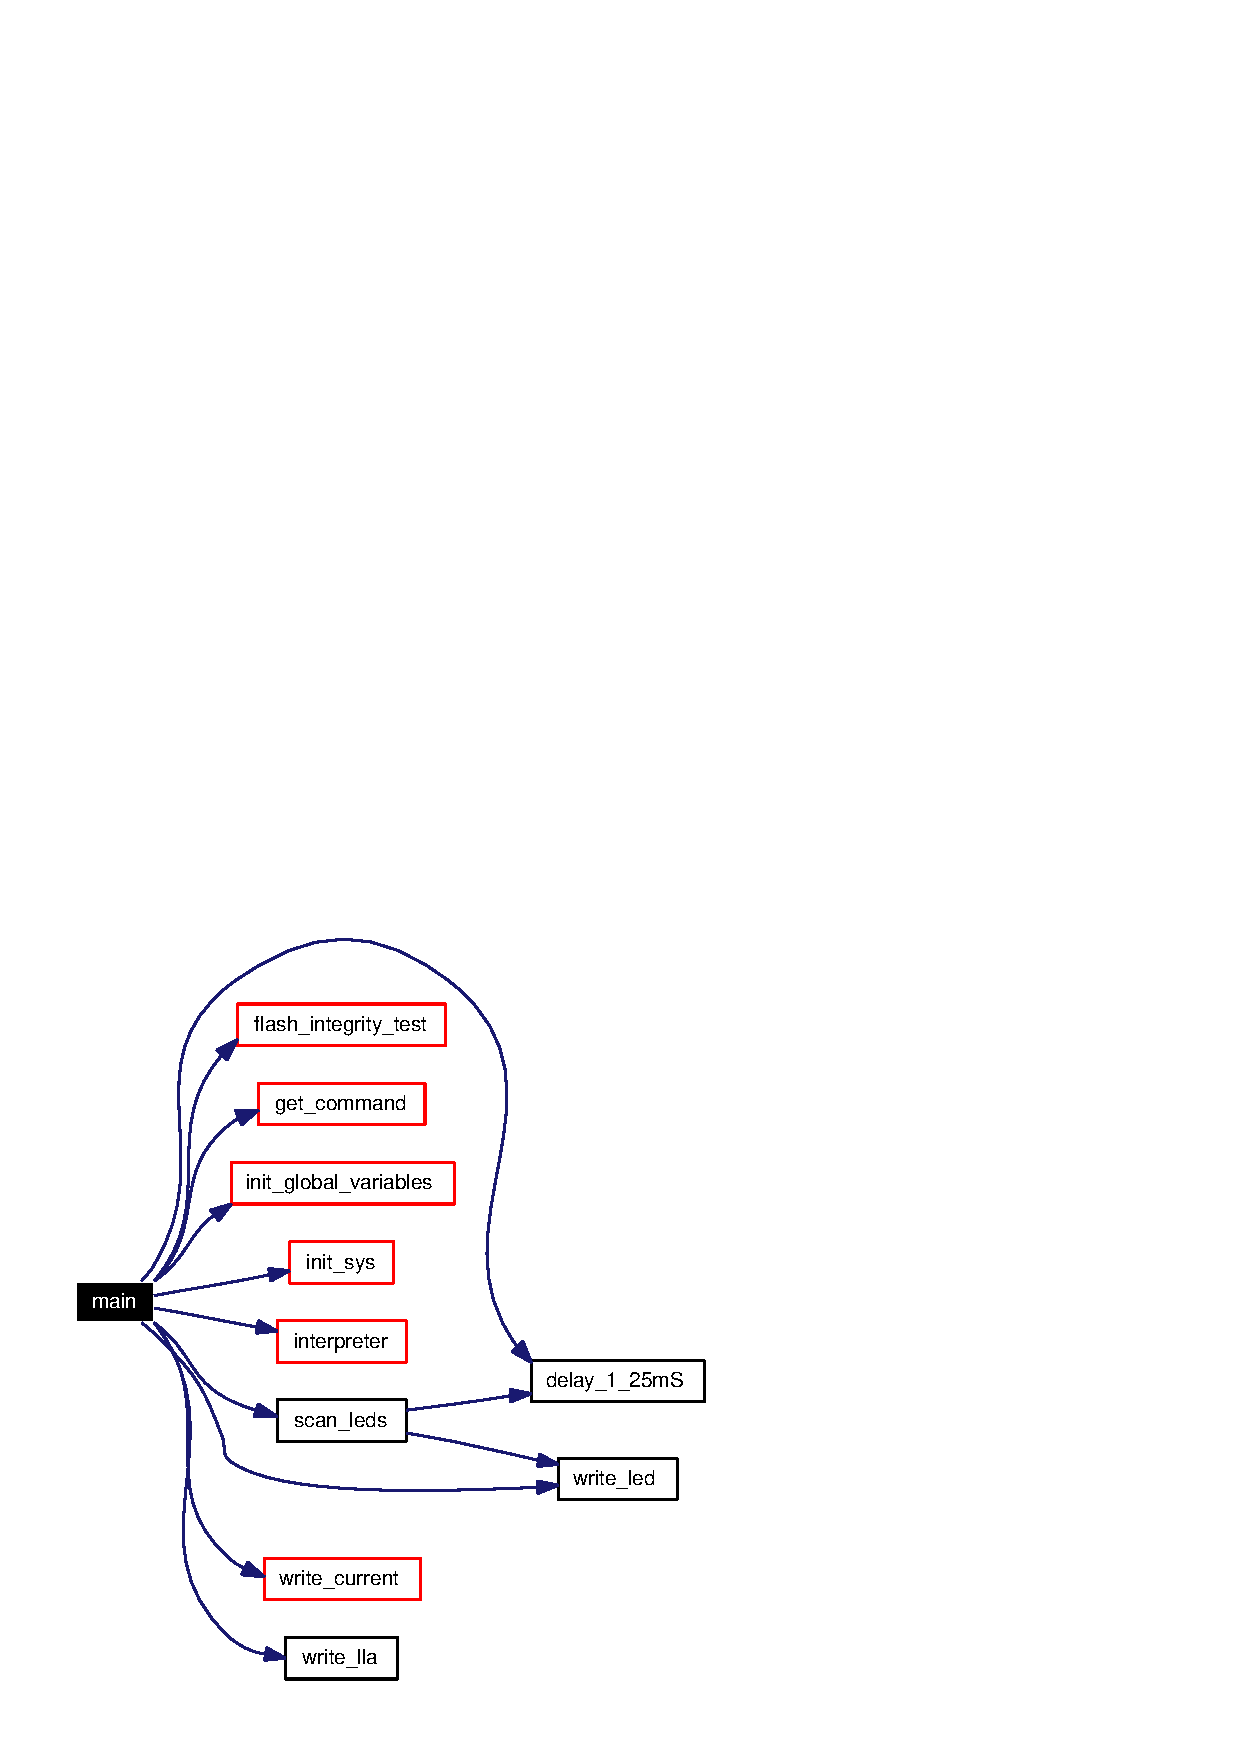
\includegraphics[width=169pt]{main_8c_a4_cgraph}
\end{center}
\end{figure}
\index{main.c@{main.c}!print_grid_i@{print\_\-grid\_\-i}}
\index{print_grid_i@{print\_\-grid\_\-i}!main.c@{main.c}}
\subsubsection{\setlength{\rightskip}{0pt plus 5cm}void print\_\-grid\_\-i ()}\label{main_8c_a2}




Definition at line 151 of file main.c.

References conversion\_\-result, convert\_\-a2d(), delay\_\-1\_\-25m\-S(), I\_\-CONVERSION, ueacval::integer, pin\_\-data, write\_\-current(), and write\_\-lla().

\footnotesize\begin{verbatim}151                     {
152   int i,j;
153   for (i=0;i<5;i++) {
154     for (j=0;j<5;j++) {
155       write_lla(i*5+j,1);
156       write_current(i*5+j,200);
157       delay_1_25mS(500);
158       convert_a2d(I_CONVERSION,pin_data[i*5+j].filtered_result,&conversion_result,i*5+j); 
159       printf("%d ",conversion_result.integer);
160       write_lla(i*5+j,0);
161     }
162     printf("\n\r");
163   }
164 }
\end{verbatim}\normalsize 




Here is the call graph for this function:\begin{figure}[H]
\begin{center}
\leavevmode
\includegraphics[width=218pt]{main_8c_a2_cgraph}
\end{center}
\end{figure}
\index{main.c@{main.c}!print_grid_v@{print\_\-grid\_\-v}}
\index{print_grid_v@{print\_\-grid\_\-v}!main.c@{main.c}}
\subsubsection{\setlength{\rightskip}{0pt plus 5cm}void print\_\-grid\_\-v ()}\label{main_8c_a1}




Definition at line 140 of file main.c.

References conversion\_\-result, convert\_\-a2d(), ueacval::hundredth, ueacval::integer, pin\_\-data, and V\_\-CONVERSION.

\footnotesize\begin{verbatim}140                     {
141   int i,j;
142   for (i=0;i<5;i++) {
143     for (j=0;j<5;j++) {
144       convert_a2d(V_CONVERSION,pin_data[i*5+j].filtered_result,&conversion_result,i*5+j); 
145       printf("%d.%d ",conversion_result.integer,conversion_result.hundredth);
146     }
147     printf("\n\r");
148   }
149 }
\end{verbatim}\normalsize 




Here is the call graph for this function:\begin{figure}[H]
\begin{center}
\leavevmode
\includegraphics[width=107pt]{main_8c_a1_cgraph}
\end{center}
\end{figure}
\index{main.c@{main.c}!scan_probes@{scan\_\-probes}}
\index{scan_probes@{scan\_\-probes}!main.c@{main.c}}
\subsubsection{\setlength{\rightskip}{0pt plus 5cm}void scan\_\-probes ()}\label{main_8c_a5}




Definition at line 113 of file main.c.

References conversion\_\-result, convert\_\-a2d(), delay\_\-1\_\-25m\-S(), I\_\-CONVERSION, ueacval::integer, pin\_\-data, write\_\-current(), and write\_\-lla().

\footnotesize\begin{verbatim}113                    {
114   int i,j;
115   for (i=0;i<25;i++) {
116     write_lla(i,1);
117     printf("%d ",i);
118     for (j=200;j>=0;j-=50) {
119       write_current(i,j);
120       delay_1_25mS(400);     
121       convert_a2d(I_CONVERSION,pin_data[i].filtered_result,&conversion_result,i);
122       printf("%d ",conversion_result.integer);
123     }
124     printf("\n\r");
125     write_lla(i,0);
126   }
127 }
\end{verbatim}\normalsize 




Here is the call graph for this function:\begin{figure}[H]
\begin{center}
\leavevmode
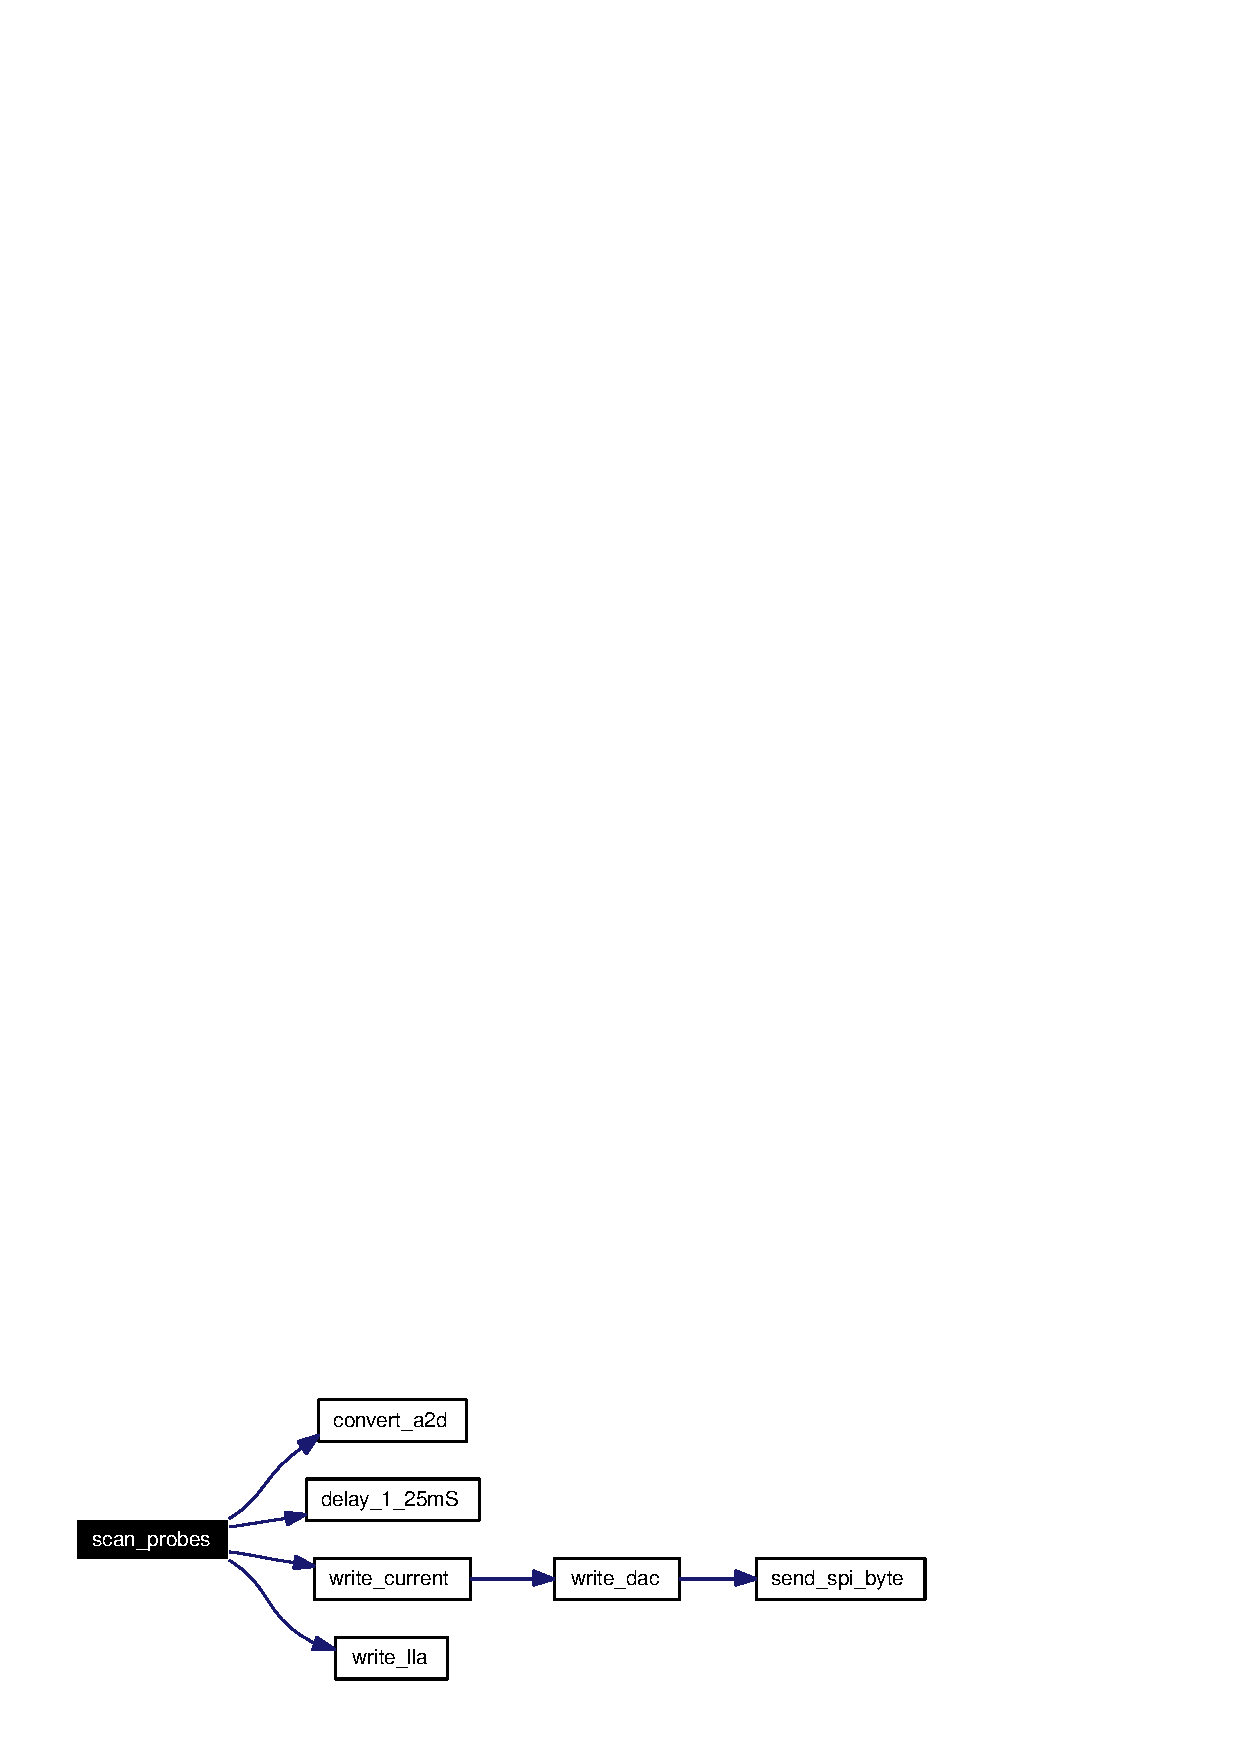
\includegraphics[width=222pt]{main_8c_a5_cgraph}
\end{center}
\end{figure}


\subsection{Variable Documentation}
\index{main.c@{main.c}!dac_translation@{dac\_\-translation}}
\index{dac_translation@{dac\_\-translation}!main.c@{main.c}}
\subsubsection{\setlength{\rightskip}{0pt plus 5cm}short {\bf dac\_\-translation}[$\,$]}\label{main_8c_a0}




Definition at line 45 of file cal\_\-table.h.
\hypertarget{power_8c}{}\section{Src/power.c File Reference}
\label{power_8c}\index{Src/power.\+c@{Src/power.\+c}}
{\ttfamily \#include \char`\"{}main.\+h\char`\"{}}\newline
{\ttfamily \#include $<$stm32l4xx\+\_\+ll\+\_\+lpuart.\+h$>$}\newline
{\ttfamily \#include $<$stdio.\+h$>$}\newline
Include dependency graph for power.\+c\+:
% FIG 0
\subsection*{Functions}
\begin{DoxyCompactItemize}
\item 
void \hyperlink{power_8c_a70af21c671abfcc773614a9a4f63d920}{System\+Clock\+\_\+\+Config} (void)
\begin{DoxyCompactList}\small\item\em System Clock Configuration. \end{DoxyCompactList}\item 
void \hyperlink{power_8c_af85df90ea394e6b7a6c0024f025ef93d}{lp\+\_\+stop\+\_\+wfi} ()
\end{DoxyCompactItemize}


\subsection{Function Documentation}
\mbox{\Hypertarget{power_8c_af85df90ea394e6b7a6c0024f025ef93d}\label{power_8c_af85df90ea394e6b7a6c0024f025ef93d}} 
\index{power.\+c@{power.\+c}!lp\+\_\+stop\+\_\+wfi@{lp\+\_\+stop\+\_\+wfi}}
\index{lp\+\_\+stop\+\_\+wfi@{lp\+\_\+stop\+\_\+wfi}!power.\+c@{power.\+c}}
\subsubsection{\texorpdfstring{lp\+\_\+stop\+\_\+wfi()}{lp\_stop\_wfi()}}
{\footnotesize\ttfamily void lp\+\_\+stop\+\_\+wfi (\begin{DoxyParamCaption}\item[{void}]{ }\end{DoxyParamCaption})}

\mbox{\Hypertarget{power_8c_a70af21c671abfcc773614a9a4f63d920}\label{power_8c_a70af21c671abfcc773614a9a4f63d920}} 
\index{power.\+c@{power.\+c}!System\+Clock\+\_\+\+Config@{System\+Clock\+\_\+\+Config}}
\index{System\+Clock\+\_\+\+Config@{System\+Clock\+\_\+\+Config}!power.\+c@{power.\+c}}
\subsubsection{\texorpdfstring{System\+Clock\+\_\+\+Config()}{SystemClock\_Config()}}
{\footnotesize\ttfamily void System\+Clock\+\_\+\+Config (\begin{DoxyParamCaption}\item[{void}]{ }\end{DoxyParamCaption})}



System Clock Configuration. 


\begin{DoxyRetVals}{Return values}
{\em None} & \\
\hline
\end{DoxyRetVals}
Initializes the C\+PU, A\+HB and A\+PB busses clocks

Initializes the C\+PU, A\+HB and A\+PB busses clocks

Configure the main internal regulator output voltage

Enable M\+SI Auto calibration
\hypertarget{pwr_8c}{}\section{Src/pwr.c File Reference}
\label{pwr_8c}\index{Src/pwr.\+c@{Src/pwr.\+c}}

\hypertarget{queue_8c}{}\section{Src/queue.c File Reference}
\label{queue_8c}\index{Src/queue.\+c@{Src/queue.\+c}}
{\ttfamily \#include \char`\"{}queue.\+h\char`\"{}}\newline
{\ttfamily \#include \char`\"{}interrupt.\+h\char`\"{}}\newline
Include dependency graph for queue.\+c\+:
% FIG 0
\subsection*{Functions}
\begin{DoxyCompactItemize}
\item 
void \hyperlink{queue_8c_ab2f2db1f35cdfb9543397181133d061a}{init\+\_\+queue} (\hyperlink{queue_8h_a410790d8f6c9a3ad1a3dbdca2e09d16a}{queue\+\_\+t} $\ast$buf)
\item 
int \hyperlink{queue_8c_aa0c8fdaa44eccd961c97e3926c955e6f}{enqueue} (\hyperlink{queue_8h_a410790d8f6c9a3ad1a3dbdca2e09d16a}{queue\+\_\+t} $\ast$buf, uint8\+\_\+t data)
\item 
uint8\+\_\+t \hyperlink{queue_8c_a6631318de511acea7f44ceba30c4efaa}{dequeue} (\hyperlink{queue_8h_a410790d8f6c9a3ad1a3dbdca2e09d16a}{queue\+\_\+t} $\ast$buf)
\item 
int \hyperlink{queue_8c_a49326f71e910976319b8bb9bc916d75c}{queue\+\_\+empty} (\hyperlink{queue_8h_a410790d8f6c9a3ad1a3dbdca2e09d16a}{queue\+\_\+t} $\ast$buf)
\end{DoxyCompactItemize}


\subsection{Function Documentation}
\mbox{\Hypertarget{queue_8c_a6631318de511acea7f44ceba30c4efaa}\label{queue_8c_a6631318de511acea7f44ceba30c4efaa}} 
\index{queue.\+c@{queue.\+c}!dequeue@{dequeue}}
\index{dequeue@{dequeue}!queue.\+c@{queue.\+c}}
\subsubsection{\texorpdfstring{dequeue()}{dequeue()}}
{\footnotesize\ttfamily uint8\+\_\+t dequeue (\begin{DoxyParamCaption}\item[{\hyperlink{queue_8h_a410790d8f6c9a3ad1a3dbdca2e09d16a}{queue\+\_\+t} $\ast$}]{buf }\end{DoxyParamCaption})}

\mbox{\Hypertarget{queue_8c_aa0c8fdaa44eccd961c97e3926c955e6f}\label{queue_8c_aa0c8fdaa44eccd961c97e3926c955e6f}} 
\index{queue.\+c@{queue.\+c}!enqueue@{enqueue}}
\index{enqueue@{enqueue}!queue.\+c@{queue.\+c}}
\subsubsection{\texorpdfstring{enqueue()}{enqueue()}}
{\footnotesize\ttfamily int enqueue (\begin{DoxyParamCaption}\item[{\hyperlink{queue_8h_a410790d8f6c9a3ad1a3dbdca2e09d16a}{queue\+\_\+t} $\ast$}]{buf,  }\item[{uint8\+\_\+t}]{data }\end{DoxyParamCaption})}

\mbox{\Hypertarget{queue_8c_ab2f2db1f35cdfb9543397181133d061a}\label{queue_8c_ab2f2db1f35cdfb9543397181133d061a}} 
\index{queue.\+c@{queue.\+c}!init\+\_\+queue@{init\+\_\+queue}}
\index{init\+\_\+queue@{init\+\_\+queue}!queue.\+c@{queue.\+c}}
\subsubsection{\texorpdfstring{init\+\_\+queue()}{init\_queue()}}
{\footnotesize\ttfamily void init\+\_\+queue (\begin{DoxyParamCaption}\item[{\hyperlink{queue_8h_a410790d8f6c9a3ad1a3dbdca2e09d16a}{queue\+\_\+t} $\ast$}]{buf }\end{DoxyParamCaption})}

\mbox{\Hypertarget{queue_8c_a49326f71e910976319b8bb9bc916d75c}\label{queue_8c_a49326f71e910976319b8bb9bc916d75c}} 
\index{queue.\+c@{queue.\+c}!queue\+\_\+empty@{queue\+\_\+empty}}
\index{queue\+\_\+empty@{queue\+\_\+empty}!queue.\+c@{queue.\+c}}
\subsubsection{\texorpdfstring{queue\+\_\+empty()}{queue\_empty()}}
{\footnotesize\ttfamily int queue\+\_\+empty (\begin{DoxyParamCaption}\item[{\hyperlink{queue_8h_a410790d8f6c9a3ad1a3dbdca2e09d16a}{queue\+\_\+t} $\ast$}]{buf }\end{DoxyParamCaption})}


\hypertarget{retarget_8c}{}\section{Src/retarget.c File Reference}
\label{retarget_8c}\index{Src/retarget.\+c@{Src/retarget.\+c}}
{\ttfamily \#include $<$\+\_\+ansi.\+h$>$}\newline
{\ttfamily \#include $<$\+\_\+syslist.\+h$>$}\newline
{\ttfamily \#include $<$errno.\+h$>$}\newline
{\ttfamily \#include $<$sys/time.\+h$>$}\newline
{\ttfamily \#include $<$sys/times.\+h$>$}\newline
{\ttfamily \#include $<$limits.\+h$>$}\newline
{\ttfamily \#include $<$signal.\+h$>$}\newline
{\ttfamily \#include $<$stdint.\+h$>$}\newline
{\ttfamily \#include $<$stdio.\+h$>$}\newline
{\ttfamily \#include \char`\"{}retarget.\+h\char`\"{}}\newline
Include dependency graph for retarget.\+c\+:
% FIG 0
\subsection*{Macros}
\begin{DoxyCompactItemize}
\item 
\#define \hyperlink{retarget_8c_afcf80a6d91178952d107ad00b165752b}{S\+T\+D\+I\+N\+\_\+\+F\+I\+L\+E\+NO}~0
\item 
\#define \hyperlink{retarget_8c_abd165ee6474b5b75bf075842fff13a04}{S\+T\+D\+O\+U\+T\+\_\+\+F\+I\+L\+E\+NO}~1
\item 
\#define \hyperlink{retarget_8c_ae2fe1725bb5e9823d089c46b9ed5266e}{S\+T\+D\+E\+R\+R\+\_\+\+F\+I\+L\+E\+NO}~2
\end{DoxyCompactItemize}
\subsection*{Functions}
\begin{DoxyCompactItemize}
\item 
void \hyperlink{retarget_8c_ac7028227e5051dfa3bb8fabb0edd07c8}{Retarget\+Init} (U\+A\+R\+T\+\_\+\+Handle\+Type\+Def $\ast$huart)
\item 
int \hyperlink{retarget_8c_a4284676ccba12d7f2061d338001f71fb}{\+\_\+isatty} (int fd)
\item 
int \hyperlink{retarget_8c_a0c1fa2d02c07b22bf2ebd769a028b852}{\+\_\+write} (int fd, char $\ast$ptr, int len)
\item 
int \hyperlink{retarget_8c_a58a559c63748012aab165d5f82af766d}{\+\_\+close} (int fd)
\item 
int \hyperlink{retarget_8c_a883d6c1f92ad3c6f19731e7b57b2c458}{\+\_\+lseek} (int fd, int ptr, int dir)
\item 
int \hyperlink{retarget_8c_ab60e5acd5530805f1421802fc0dc1d35}{\+\_\+read} (int fd, char $\ast$ptr, int len)
\item 
int \hyperlink{retarget_8c_a6e8d95db883bc4efe10c487d74e96b06}{\+\_\+fstat} (int fd, struct stat $\ast$st)
\end{DoxyCompactItemize}
\subsection*{Variables}
\begin{DoxyCompactItemize}
\item 
U\+A\+R\+T\+\_\+\+Handle\+Type\+Def $\ast$ \hyperlink{retarget_8c_af8d99acb61924bc42b4652c2316c1b20}{g\+Huart}
\end{DoxyCompactItemize}


\subsection{Macro Definition Documentation}
\mbox{\Hypertarget{retarget_8c_ae2fe1725bb5e9823d089c46b9ed5266e}\label{retarget_8c_ae2fe1725bb5e9823d089c46b9ed5266e}} 
\index{retarget.\+c@{retarget.\+c}!S\+T\+D\+E\+R\+R\+\_\+\+F\+I\+L\+E\+NO@{S\+T\+D\+E\+R\+R\+\_\+\+F\+I\+L\+E\+NO}}
\index{S\+T\+D\+E\+R\+R\+\_\+\+F\+I\+L\+E\+NO@{S\+T\+D\+E\+R\+R\+\_\+\+F\+I\+L\+E\+NO}!retarget.\+c@{retarget.\+c}}
\subsubsection{\texorpdfstring{S\+T\+D\+E\+R\+R\+\_\+\+F\+I\+L\+E\+NO}{STDERR\_FILENO}}
{\footnotesize\ttfamily \#define S\+T\+D\+E\+R\+R\+\_\+\+F\+I\+L\+E\+NO~2}

\mbox{\Hypertarget{retarget_8c_afcf80a6d91178952d107ad00b165752b}\label{retarget_8c_afcf80a6d91178952d107ad00b165752b}} 
\index{retarget.\+c@{retarget.\+c}!S\+T\+D\+I\+N\+\_\+\+F\+I\+L\+E\+NO@{S\+T\+D\+I\+N\+\_\+\+F\+I\+L\+E\+NO}}
\index{S\+T\+D\+I\+N\+\_\+\+F\+I\+L\+E\+NO@{S\+T\+D\+I\+N\+\_\+\+F\+I\+L\+E\+NO}!retarget.\+c@{retarget.\+c}}
\subsubsection{\texorpdfstring{S\+T\+D\+I\+N\+\_\+\+F\+I\+L\+E\+NO}{STDIN\_FILENO}}
{\footnotesize\ttfamily \#define S\+T\+D\+I\+N\+\_\+\+F\+I\+L\+E\+NO~0}

\mbox{\Hypertarget{retarget_8c_abd165ee6474b5b75bf075842fff13a04}\label{retarget_8c_abd165ee6474b5b75bf075842fff13a04}} 
\index{retarget.\+c@{retarget.\+c}!S\+T\+D\+O\+U\+T\+\_\+\+F\+I\+L\+E\+NO@{S\+T\+D\+O\+U\+T\+\_\+\+F\+I\+L\+E\+NO}}
\index{S\+T\+D\+O\+U\+T\+\_\+\+F\+I\+L\+E\+NO@{S\+T\+D\+O\+U\+T\+\_\+\+F\+I\+L\+E\+NO}!retarget.\+c@{retarget.\+c}}
\subsubsection{\texorpdfstring{S\+T\+D\+O\+U\+T\+\_\+\+F\+I\+L\+E\+NO}{STDOUT\_FILENO}}
{\footnotesize\ttfamily \#define S\+T\+D\+O\+U\+T\+\_\+\+F\+I\+L\+E\+NO~1}



\subsection{Function Documentation}
\mbox{\Hypertarget{retarget_8c_a58a559c63748012aab165d5f82af766d}\label{retarget_8c_a58a559c63748012aab165d5f82af766d}} 
\index{retarget.\+c@{retarget.\+c}!\+\_\+close@{\+\_\+close}}
\index{\+\_\+close@{\+\_\+close}!retarget.\+c@{retarget.\+c}}
\subsubsection{\texorpdfstring{\+\_\+close()}{\_close()}}
{\footnotesize\ttfamily int \+\_\+close (\begin{DoxyParamCaption}\item[{int}]{fd }\end{DoxyParamCaption})}

\mbox{\Hypertarget{retarget_8c_a6e8d95db883bc4efe10c487d74e96b06}\label{retarget_8c_a6e8d95db883bc4efe10c487d74e96b06}} 
\index{retarget.\+c@{retarget.\+c}!\+\_\+fstat@{\+\_\+fstat}}
\index{\+\_\+fstat@{\+\_\+fstat}!retarget.\+c@{retarget.\+c}}
\subsubsection{\texorpdfstring{\+\_\+fstat()}{\_fstat()}}
{\footnotesize\ttfamily int \+\_\+fstat (\begin{DoxyParamCaption}\item[{int}]{fd,  }\item[{struct stat $\ast$}]{st }\end{DoxyParamCaption})}

\mbox{\Hypertarget{retarget_8c_a4284676ccba12d7f2061d338001f71fb}\label{retarget_8c_a4284676ccba12d7f2061d338001f71fb}} 
\index{retarget.\+c@{retarget.\+c}!\+\_\+isatty@{\+\_\+isatty}}
\index{\+\_\+isatty@{\+\_\+isatty}!retarget.\+c@{retarget.\+c}}
\subsubsection{\texorpdfstring{\+\_\+isatty()}{\_isatty()}}
{\footnotesize\ttfamily int \+\_\+isatty (\begin{DoxyParamCaption}\item[{int}]{fd }\end{DoxyParamCaption})}

\mbox{\Hypertarget{retarget_8c_a883d6c1f92ad3c6f19731e7b57b2c458}\label{retarget_8c_a883d6c1f92ad3c6f19731e7b57b2c458}} 
\index{retarget.\+c@{retarget.\+c}!\+\_\+lseek@{\+\_\+lseek}}
\index{\+\_\+lseek@{\+\_\+lseek}!retarget.\+c@{retarget.\+c}}
\subsubsection{\texorpdfstring{\+\_\+lseek()}{\_lseek()}}
{\footnotesize\ttfamily int \+\_\+lseek (\begin{DoxyParamCaption}\item[{int}]{fd,  }\item[{int}]{ptr,  }\item[{int}]{dir }\end{DoxyParamCaption})}

\mbox{\Hypertarget{retarget_8c_ab60e5acd5530805f1421802fc0dc1d35}\label{retarget_8c_ab60e5acd5530805f1421802fc0dc1d35}} 
\index{retarget.\+c@{retarget.\+c}!\+\_\+read@{\+\_\+read}}
\index{\+\_\+read@{\+\_\+read}!retarget.\+c@{retarget.\+c}}
\subsubsection{\texorpdfstring{\+\_\+read()}{\_read()}}
{\footnotesize\ttfamily int \+\_\+read (\begin{DoxyParamCaption}\item[{int}]{fd,  }\item[{char $\ast$}]{ptr,  }\item[{int}]{len }\end{DoxyParamCaption})}

\mbox{\Hypertarget{retarget_8c_a0c1fa2d02c07b22bf2ebd769a028b852}\label{retarget_8c_a0c1fa2d02c07b22bf2ebd769a028b852}} 
\index{retarget.\+c@{retarget.\+c}!\+\_\+write@{\+\_\+write}}
\index{\+\_\+write@{\+\_\+write}!retarget.\+c@{retarget.\+c}}
\subsubsection{\texorpdfstring{\+\_\+write()}{\_write()}}
{\footnotesize\ttfamily int \+\_\+write (\begin{DoxyParamCaption}\item[{int}]{fd,  }\item[{char $\ast$}]{ptr,  }\item[{int}]{len }\end{DoxyParamCaption})}

\mbox{\Hypertarget{retarget_8c_ac7028227e5051dfa3bb8fabb0edd07c8}\label{retarget_8c_ac7028227e5051dfa3bb8fabb0edd07c8}} 
\index{retarget.\+c@{retarget.\+c}!Retarget\+Init@{Retarget\+Init}}
\index{Retarget\+Init@{Retarget\+Init}!retarget.\+c@{retarget.\+c}}
\subsubsection{\texorpdfstring{Retarget\+Init()}{RetargetInit()}}
{\footnotesize\ttfamily void Retarget\+Init (\begin{DoxyParamCaption}\item[{U\+A\+R\+T\+\_\+\+Handle\+Type\+Def $\ast$}]{huart }\end{DoxyParamCaption})}



\subsection{Variable Documentation}
\mbox{\Hypertarget{retarget_8c_af8d99acb61924bc42b4652c2316c1b20}\label{retarget_8c_af8d99acb61924bc42b4652c2316c1b20}} 
\index{retarget.\+c@{retarget.\+c}!g\+Huart@{g\+Huart}}
\index{g\+Huart@{g\+Huart}!retarget.\+c@{retarget.\+c}}
\subsubsection{\texorpdfstring{g\+Huart}{gHuart}}
{\footnotesize\ttfamily U\+A\+R\+T\+\_\+\+Handle\+Type\+Def$\ast$ g\+Huart}


\hypertarget{rtc_8c}{}\section{Src/rtc.c File Reference}
\label{rtc_8c}\index{Src/rtc.\+c@{Src/rtc.\+c}}
{\ttfamily \#include \char`\"{}main.\+h\char`\"{}}\newline
{\ttfamily \#include $<$stdio.\+h$>$}\newline
{\ttfamily \#include $<$string.\+h$>$}\newline
{\ttfamily \#include $<$stdlib.\+h$>$}\newline
{\ttfamily \#include \char`\"{}rtc.\+h\char`\"{}}\newline
Include dependency graph for rtc.\+c\+:
% FIG 0
\subsection*{Functions}
\begin{DoxyCompactItemize}
\item 
void \hyperlink{rtc_8c_abbeb82818425ce05fa4510455ffcbda5}{ds\+\_\+command} (char $\ast$arguments)
\item 
void \hyperlink{rtc_8c_abd818ebb099d573647a39b8f96252dbc}{ts\+\_\+command} (char $\ast$arguments)
\item 
void \hyperlink{rtc_8c_aa4374d45e6be2570a7e9d7c5f5435f78}{tr\+\_\+command} (char $\ast$arguments)
\item 
void \hyperlink{rtc_8c_aaec93ce711d91fb6867fa0b855f53910}{dr\+\_\+command} (char $\ast$arguments)
\item 
uint32\+\_\+t \hyperlink{rtc_8c_a701619892591e5cd5b242b83cb16eec8}{pack\+\_\+time} (R\+T\+C\+\_\+\+Time\+Type\+Def $\ast$time, R\+T\+C\+\_\+\+Date\+Type\+Def $\ast$date)
\item 
void \hyperlink{rtc_8c_a953d4ca458b5a21c4e4e450cb9ba9fab}{unpack\+\_\+time} (uint32\+\_\+t timeval, R\+T\+C\+\_\+\+Time\+Type\+Def $\ast$time, R\+T\+C\+\_\+\+Date\+Type\+Def $\ast$date)
\end{DoxyCompactItemize}
\subsection*{Variables}
\begin{DoxyCompactItemize}
\item 
R\+T\+C\+\_\+\+Handle\+Type\+Def \hyperlink{rtc_8c_aa0c7fca836406ade332e1e3f1039d8ab}{hrtc}
\end{DoxyCompactItemize}


\subsection{Function Documentation}
\mbox{\Hypertarget{rtc_8c_aaec93ce711d91fb6867fa0b855f53910}\label{rtc_8c_aaec93ce711d91fb6867fa0b855f53910}} 
\index{rtc.\+c@{rtc.\+c}!dr\+\_\+command@{dr\+\_\+command}}
\index{dr\+\_\+command@{dr\+\_\+command}!rtc.\+c@{rtc.\+c}}
\subsubsection{\texorpdfstring{dr\+\_\+command()}{dr\_command()}}
{\footnotesize\ttfamily void dr\+\_\+command (\begin{DoxyParamCaption}\item[{char $\ast$}]{arguments }\end{DoxyParamCaption})}

\mbox{\Hypertarget{rtc_8c_abbeb82818425ce05fa4510455ffcbda5}\label{rtc_8c_abbeb82818425ce05fa4510455ffcbda5}} 
\index{rtc.\+c@{rtc.\+c}!ds\+\_\+command@{ds\+\_\+command}}
\index{ds\+\_\+command@{ds\+\_\+command}!rtc.\+c@{rtc.\+c}}
\subsubsection{\texorpdfstring{ds\+\_\+command()}{ds\_command()}}
{\footnotesize\ttfamily void ds\+\_\+command (\begin{DoxyParamCaption}\item[{char $\ast$}]{arguments }\end{DoxyParamCaption})}

\mbox{\Hypertarget{rtc_8c_a701619892591e5cd5b242b83cb16eec8}\label{rtc_8c_a701619892591e5cd5b242b83cb16eec8}} 
\index{rtc.\+c@{rtc.\+c}!pack\+\_\+time@{pack\+\_\+time}}
\index{pack\+\_\+time@{pack\+\_\+time}!rtc.\+c@{rtc.\+c}}
\subsubsection{\texorpdfstring{pack\+\_\+time()}{pack\_time()}}
{\footnotesize\ttfamily uint32\+\_\+t pack\+\_\+time (\begin{DoxyParamCaption}\item[{R\+T\+C\+\_\+\+Time\+Type\+Def $\ast$}]{time,  }\item[{R\+T\+C\+\_\+\+Date\+Type\+Def $\ast$}]{date }\end{DoxyParamCaption})}

\mbox{\Hypertarget{rtc_8c_aa4374d45e6be2570a7e9d7c5f5435f78}\label{rtc_8c_aa4374d45e6be2570a7e9d7c5f5435f78}} 
\index{rtc.\+c@{rtc.\+c}!tr\+\_\+command@{tr\+\_\+command}}
\index{tr\+\_\+command@{tr\+\_\+command}!rtc.\+c@{rtc.\+c}}
\subsubsection{\texorpdfstring{tr\+\_\+command()}{tr\_command()}}
{\footnotesize\ttfamily void tr\+\_\+command (\begin{DoxyParamCaption}\item[{char $\ast$}]{arguments }\end{DoxyParamCaption})}

\mbox{\Hypertarget{rtc_8c_abd818ebb099d573647a39b8f96252dbc}\label{rtc_8c_abd818ebb099d573647a39b8f96252dbc}} 
\index{rtc.\+c@{rtc.\+c}!ts\+\_\+command@{ts\+\_\+command}}
\index{ts\+\_\+command@{ts\+\_\+command}!rtc.\+c@{rtc.\+c}}
\subsubsection{\texorpdfstring{ts\+\_\+command()}{ts\_command()}}
{\footnotesize\ttfamily void ts\+\_\+command (\begin{DoxyParamCaption}\item[{char $\ast$}]{arguments }\end{DoxyParamCaption})}

\mbox{\Hypertarget{rtc_8c_a953d4ca458b5a21c4e4e450cb9ba9fab}\label{rtc_8c_a953d4ca458b5a21c4e4e450cb9ba9fab}} 
\index{rtc.\+c@{rtc.\+c}!unpack\+\_\+time@{unpack\+\_\+time}}
\index{unpack\+\_\+time@{unpack\+\_\+time}!rtc.\+c@{rtc.\+c}}
\subsubsection{\texorpdfstring{unpack\+\_\+time()}{unpack\_time()}}
{\footnotesize\ttfamily void unpack\+\_\+time (\begin{DoxyParamCaption}\item[{uint32\+\_\+t}]{timeval,  }\item[{R\+T\+C\+\_\+\+Time\+Type\+Def $\ast$}]{time,  }\item[{R\+T\+C\+\_\+\+Date\+Type\+Def $\ast$}]{date }\end{DoxyParamCaption})}



\subsection{Variable Documentation}
\mbox{\Hypertarget{rtc_8c_aa0c7fca836406ade332e1e3f1039d8ab}\label{rtc_8c_aa0c7fca836406ade332e1e3f1039d8ab}} 
\index{rtc.\+c@{rtc.\+c}!hrtc@{hrtc}}
\index{hrtc@{hrtc}!rtc.\+c@{rtc.\+c}}
\subsubsection{\texorpdfstring{hrtc}{hrtc}}
{\footnotesize\ttfamily R\+T\+C\+\_\+\+Handle\+Type\+Def hrtc}


\hypertarget{sample_8c}{}\section{Src/sample.c File Reference}
\label{sample_8c}\index{Src/sample.\+c@{Src/sample.\+c}}
{\ttfamily \#include \char`\"{}main.\+h\char`\"{}}\newline
{\ttfamily \#include $<$stdio.\+h$>$}\newline
{\ttfamily \#include $<$stdint.\+h$>$}\newline
{\ttfamily \#include $<$string.\+h$>$}\newline
{\ttfamily \#include \char`\"{}flash.\+h\char`\"{}}\newline
{\ttfamily \#include \char`\"{}rtc.\+h\char`\"{}}\newline
{\ttfamily \#include \char`\"{}battery.\+h\char`\"{}}\newline
{\ttfamily \#include \char`\"{}temperature.\+h\char`\"{}}\newline
{\ttfamily \#include \char`\"{}tsl237.\+h\char`\"{}}\newline
{\ttfamily \#include \char`\"{}sample.\+h\char`\"{}}\newline
Include dependency graph for sample.\+c\+:
% FIG 0
\subsection*{Functions}
\begin{DoxyCompactItemize}
\item 
void \hyperlink{sample_8c_ac4e76bb6286287d38bbabe01000114fa}{sample\+\_\+command} (char $\ast$arguments)
\item 
void \hyperlink{sample_8c_aace51f3aed145d5c5ab51963f5484ed7}{sample} (void)
\item 
uint32\+\_\+t \hyperlink{sample_8c_a4e35fbb49655630ac541f3e950649b05}{sample\+\_\+noflash} (void)
\end{DoxyCompactItemize}
\subsection*{Variables}
\begin{DoxyCompactItemize}
\item 
\hyperlink{flash_8h_a813b2c2faae1816ffd6890a96f75dc97}{flash\+\_\+status\+\_\+t} \hyperlink{sample_8c_af103e485f895120eef7c5b0624f6a88c}{fs}
\item 
A\+D\+C\+\_\+\+Handle\+Type\+Def \hyperlink{sample_8c_a22b804736f5648d52f639b2647d4ed13}{hadc1}
\item 
T\+I\+M\+\_\+\+Handle\+Type\+Def \hyperlink{sample_8c_a2c80fd5510e2990a59a5c90d745c716c}{htim2}
\end{DoxyCompactItemize}


\subsection{Function Documentation}
\mbox{\Hypertarget{sample_8c_aace51f3aed145d5c5ab51963f5484ed7}\label{sample_8c_aace51f3aed145d5c5ab51963f5484ed7}} 
\index{sample.\+c@{sample.\+c}!sample@{sample}}
\index{sample@{sample}!sample.\+c@{sample.\+c}}
\subsubsection{\texorpdfstring{sample()}{sample()}}
{\footnotesize\ttfamily void sample (\begin{DoxyParamCaption}\item[{void}]{ }\end{DoxyParamCaption})}

\mbox{\Hypertarget{sample_8c_ac4e76bb6286287d38bbabe01000114fa}\label{sample_8c_ac4e76bb6286287d38bbabe01000114fa}} 
\index{sample.\+c@{sample.\+c}!sample\+\_\+command@{sample\+\_\+command}}
\index{sample\+\_\+command@{sample\+\_\+command}!sample.\+c@{sample.\+c}}
\subsubsection{\texorpdfstring{sample\+\_\+command()}{sample\_command()}}
{\footnotesize\ttfamily void sample\+\_\+command (\begin{DoxyParamCaption}\item[{char $\ast$}]{arguments }\end{DoxyParamCaption})}

\mbox{\Hypertarget{sample_8c_a4e35fbb49655630ac541f3e950649b05}\label{sample_8c_a4e35fbb49655630ac541f3e950649b05}} 
\index{sample.\+c@{sample.\+c}!sample\+\_\+noflash@{sample\+\_\+noflash}}
\index{sample\+\_\+noflash@{sample\+\_\+noflash}!sample.\+c@{sample.\+c}}
\subsubsection{\texorpdfstring{sample\+\_\+noflash()}{sample\_noflash()}}
{\footnotesize\ttfamily uint32\+\_\+t sample\+\_\+noflash (\begin{DoxyParamCaption}\item[{void}]{ }\end{DoxyParamCaption})}



\subsection{Variable Documentation}
\mbox{\Hypertarget{sample_8c_af103e485f895120eef7c5b0624f6a88c}\label{sample_8c_af103e485f895120eef7c5b0624f6a88c}} 
\index{sample.\+c@{sample.\+c}!fs@{fs}}
\index{fs@{fs}!sample.\+c@{sample.\+c}}
\subsubsection{\texorpdfstring{fs}{fs}}
{\footnotesize\ttfamily \hyperlink{flash_8h_a813b2c2faae1816ffd6890a96f75dc97}{flash\+\_\+status\+\_\+t} fs}

\mbox{\Hypertarget{sample_8c_a22b804736f5648d52f639b2647d4ed13}\label{sample_8c_a22b804736f5648d52f639b2647d4ed13}} 
\index{sample.\+c@{sample.\+c}!hadc1@{hadc1}}
\index{hadc1@{hadc1}!sample.\+c@{sample.\+c}}
\subsubsection{\texorpdfstring{hadc1}{hadc1}}
{\footnotesize\ttfamily A\+D\+C\+\_\+\+Handle\+Type\+Def hadc1}

\mbox{\Hypertarget{sample_8c_a2c80fd5510e2990a59a5c90d745c716c}\label{sample_8c_a2c80fd5510e2990a59a5c90d745c716c}} 
\index{sample.\+c@{sample.\+c}!htim2@{htim2}}
\index{htim2@{htim2}!sample.\+c@{sample.\+c}}
\subsubsection{\texorpdfstring{htim2}{htim2}}
{\footnotesize\ttfamily T\+I\+M\+\_\+\+Handle\+Type\+Def htim2}


\hypertarget{stm32l4xx__hal__msp_8c}{}\section{Src/stm32l4xx\+\_\+hal\+\_\+msp.c File Reference}
\label{stm32l4xx__hal__msp_8c}\index{Src/stm32l4xx\+\_\+hal\+\_\+msp.\+c@{Src/stm32l4xx\+\_\+hal\+\_\+msp.\+c}}
{\ttfamily \#include \char`\"{}main.\+h\char`\"{}}\newline
Include dependency graph for stm32l4xx\+\_\+hal\+\_\+msp.\+c\+:
% FIG 0
\subsection*{Functions}
\begin{DoxyCompactItemize}
\item 
void \hyperlink{stm32l4xx__hal__msp_8c_ae4fb8e66865c87d0ebab74a726a6891f}{H\+A\+L\+\_\+\+Msp\+Init} (void)
\item 
void \hyperlink{stm32l4xx__hal__msp_8c_aa30863492d5c3103e3e8ce8a63dadd07}{H\+A\+L\+\_\+\+A\+D\+C\+\_\+\+Msp\+Init} (A\+D\+C\+\_\+\+Handle\+Type\+Def $\ast$hadc)
\begin{DoxyCompactList}\small\item\em A\+DC M\+SP Initialization This function configures the hardware resources used in this example. \end{DoxyCompactList}\item 
void \hyperlink{stm32l4xx__hal__msp_8c_a39b0f8e80268ab3e660ead921ad4b22f}{H\+A\+L\+\_\+\+A\+D\+C\+\_\+\+Msp\+De\+Init} (A\+D\+C\+\_\+\+Handle\+Type\+Def $\ast$hadc)
\begin{DoxyCompactList}\small\item\em A\+DC M\+SP De-\/\+Initialization This function freeze the hardware resources used in this example. \end{DoxyCompactList}\item 
void \hyperlink{stm32l4xx__hal__msp_8c_abe01a202c27b23fc150aa66af3130073}{H\+A\+L\+\_\+\+I2\+C\+\_\+\+Msp\+Init} (I2\+C\+\_\+\+Handle\+Type\+Def $\ast$hi2c)
\begin{DoxyCompactList}\small\item\em I2C M\+SP Initialization This function configures the hardware resources used in this example. \end{DoxyCompactList}\item 
void \hyperlink{stm32l4xx__hal__msp_8c_a2ec8d9b09854c732e2feed549278f048}{H\+A\+L\+\_\+\+I2\+C\+\_\+\+Msp\+De\+Init} (I2\+C\+\_\+\+Handle\+Type\+Def $\ast$hi2c)
\begin{DoxyCompactList}\small\item\em I2C M\+SP De-\/\+Initialization This function freeze the hardware resources used in this example. \end{DoxyCompactList}\item 
void \hyperlink{stm32l4xx__hal__msp_8c_a0e553b32211877322f949b14801bbfa7}{H\+A\+L\+\_\+\+U\+A\+R\+T\+\_\+\+Msp\+Init} (U\+A\+R\+T\+\_\+\+Handle\+Type\+Def $\ast$huart)
\begin{DoxyCompactList}\small\item\em U\+A\+RT M\+SP Initialization This function configures the hardware resources used in this example. \end{DoxyCompactList}\item 
void \hyperlink{stm32l4xx__hal__msp_8c_a718f39804e3b910d738a0e1e46151188}{H\+A\+L\+\_\+\+U\+A\+R\+T\+\_\+\+Msp\+De\+Init} (U\+A\+R\+T\+\_\+\+Handle\+Type\+Def $\ast$huart)
\begin{DoxyCompactList}\small\item\em U\+A\+RT M\+SP De-\/\+Initialization This function freeze the hardware resources used in this example. \end{DoxyCompactList}\item 
void \hyperlink{stm32l4xx__hal__msp_8c_aee6eddaa309c8c9829f1ca794d8f99c5}{H\+A\+L\+\_\+\+R\+T\+C\+\_\+\+Msp\+Init} (R\+T\+C\+\_\+\+Handle\+Type\+Def $\ast$\hyperlink{stm32l4xx__it_8c_aa0c7fca836406ade332e1e3f1039d8ab}{hrtc})
\begin{DoxyCompactList}\small\item\em R\+TC M\+SP Initialization This function configures the hardware resources used in this example. \end{DoxyCompactList}\item 
void \hyperlink{stm32l4xx__hal__msp_8c_a8767bc3a4d472d39a688090ab10ba6ce}{H\+A\+L\+\_\+\+R\+T\+C\+\_\+\+Msp\+De\+Init} (R\+T\+C\+\_\+\+Handle\+Type\+Def $\ast$\hyperlink{stm32l4xx__it_8c_aa0c7fca836406ade332e1e3f1039d8ab}{hrtc})
\begin{DoxyCompactList}\small\item\em R\+TC M\+SP De-\/\+Initialization This function freeze the hardware resources used in this example. \end{DoxyCompactList}\item 
void \hyperlink{stm32l4xx__hal__msp_8c_abb25ade2f7e3f7aae167bd52270c2b86}{H\+A\+L\+\_\+\+T\+I\+M\+\_\+\+Base\+\_\+\+Msp\+Init} (T\+I\+M\+\_\+\+Handle\+Type\+Def $\ast$htim\+\_\+base)
\begin{DoxyCompactList}\small\item\em T\+I\+M\+\_\+\+Base M\+SP Initialization This function configures the hardware resources used in this example. \end{DoxyCompactList}\item 
void \hyperlink{stm32l4xx__hal__msp_8c_a555b8a2d3c7a07341f8cb1255318fa2b}{H\+A\+L\+\_\+\+T\+I\+M\+\_\+\+Base\+\_\+\+Msp\+De\+Init} (T\+I\+M\+\_\+\+Handle\+Type\+Def $\ast$htim\+\_\+base)
\begin{DoxyCompactList}\small\item\em T\+I\+M\+\_\+\+Base M\+SP De-\/\+Initialization This function freeze the hardware resources used in this example. \end{DoxyCompactList}\end{DoxyCompactItemize}
\subsection*{Variables}
\begin{DoxyCompactItemize}
\item 
D\+M\+A\+\_\+\+Handle\+Type\+Def \hyperlink{stm32l4xx__hal__msp_8c_ab051b95fbef5ff0c90c0782a26ab85ba}{hdma\+\_\+tim2\+\_\+ch1}
\item 
D\+M\+A\+\_\+\+Handle\+Type\+Def \hyperlink{stm32l4xx__hal__msp_8c_ade328c372e5c1f34a2e0abe017fff447}{hdma\+\_\+tim2\+\_\+ch2\+\_\+ch4}
\end{DoxyCompactItemize}


\subsection{Function Documentation}
\mbox{\Hypertarget{stm32l4xx__hal__msp_8c_a39b0f8e80268ab3e660ead921ad4b22f}\label{stm32l4xx__hal__msp_8c_a39b0f8e80268ab3e660ead921ad4b22f}} 
\index{stm32l4xx\+\_\+hal\+\_\+msp.\+c@{stm32l4xx\+\_\+hal\+\_\+msp.\+c}!H\+A\+L\+\_\+\+A\+D\+C\+\_\+\+Msp\+De\+Init@{H\+A\+L\+\_\+\+A\+D\+C\+\_\+\+Msp\+De\+Init}}
\index{H\+A\+L\+\_\+\+A\+D\+C\+\_\+\+Msp\+De\+Init@{H\+A\+L\+\_\+\+A\+D\+C\+\_\+\+Msp\+De\+Init}!stm32l4xx\+\_\+hal\+\_\+msp.\+c@{stm32l4xx\+\_\+hal\+\_\+msp.\+c}}
\subsubsection{\texorpdfstring{H\+A\+L\+\_\+\+A\+D\+C\+\_\+\+Msp\+De\+Init()}{HAL\_ADC\_MspDeInit()}}
{\footnotesize\ttfamily void H\+A\+L\+\_\+\+A\+D\+C\+\_\+\+Msp\+De\+Init (\begin{DoxyParamCaption}\item[{A\+D\+C\+\_\+\+Handle\+Type\+Def $\ast$}]{hadc }\end{DoxyParamCaption})}



A\+DC M\+SP De-\/\+Initialization This function freeze the hardware resources used in this example. 


\begin{DoxyParams}{Parameters}
{\em hadc} & A\+DC handle pointer \\
\hline
\end{DoxyParams}

\begin{DoxyRetVals}{Return values}
{\em None} & \\
\hline
\end{DoxyRetVals}
\mbox{\Hypertarget{stm32l4xx__hal__msp_8c_aa30863492d5c3103e3e8ce8a63dadd07}\label{stm32l4xx__hal__msp_8c_aa30863492d5c3103e3e8ce8a63dadd07}} 
\index{stm32l4xx\+\_\+hal\+\_\+msp.\+c@{stm32l4xx\+\_\+hal\+\_\+msp.\+c}!H\+A\+L\+\_\+\+A\+D\+C\+\_\+\+Msp\+Init@{H\+A\+L\+\_\+\+A\+D\+C\+\_\+\+Msp\+Init}}
\index{H\+A\+L\+\_\+\+A\+D\+C\+\_\+\+Msp\+Init@{H\+A\+L\+\_\+\+A\+D\+C\+\_\+\+Msp\+Init}!stm32l4xx\+\_\+hal\+\_\+msp.\+c@{stm32l4xx\+\_\+hal\+\_\+msp.\+c}}
\subsubsection{\texorpdfstring{H\+A\+L\+\_\+\+A\+D\+C\+\_\+\+Msp\+Init()}{HAL\_ADC\_MspInit()}}
{\footnotesize\ttfamily void H\+A\+L\+\_\+\+A\+D\+C\+\_\+\+Msp\+Init (\begin{DoxyParamCaption}\item[{A\+D\+C\+\_\+\+Handle\+Type\+Def $\ast$}]{hadc }\end{DoxyParamCaption})}



A\+DC M\+SP Initialization This function configures the hardware resources used in this example. 


\begin{DoxyParams}{Parameters}
{\em hadc} & A\+DC handle pointer \\
\hline
\end{DoxyParams}

\begin{DoxyRetVals}{Return values}
{\em None} & \\
\hline
\end{DoxyRetVals}
\mbox{\Hypertarget{stm32l4xx__hal__msp_8c_a2ec8d9b09854c732e2feed549278f048}\label{stm32l4xx__hal__msp_8c_a2ec8d9b09854c732e2feed549278f048}} 
\index{stm32l4xx\+\_\+hal\+\_\+msp.\+c@{stm32l4xx\+\_\+hal\+\_\+msp.\+c}!H\+A\+L\+\_\+\+I2\+C\+\_\+\+Msp\+De\+Init@{H\+A\+L\+\_\+\+I2\+C\+\_\+\+Msp\+De\+Init}}
\index{H\+A\+L\+\_\+\+I2\+C\+\_\+\+Msp\+De\+Init@{H\+A\+L\+\_\+\+I2\+C\+\_\+\+Msp\+De\+Init}!stm32l4xx\+\_\+hal\+\_\+msp.\+c@{stm32l4xx\+\_\+hal\+\_\+msp.\+c}}
\subsubsection{\texorpdfstring{H\+A\+L\+\_\+\+I2\+C\+\_\+\+Msp\+De\+Init()}{HAL\_I2C\_MspDeInit()}}
{\footnotesize\ttfamily void H\+A\+L\+\_\+\+I2\+C\+\_\+\+Msp\+De\+Init (\begin{DoxyParamCaption}\item[{I2\+C\+\_\+\+Handle\+Type\+Def $\ast$}]{hi2c }\end{DoxyParamCaption})}



I2C M\+SP De-\/\+Initialization This function freeze the hardware resources used in this example. 


\begin{DoxyParams}{Parameters}
{\em hi2c} & I2C handle pointer \\
\hline
\end{DoxyParams}

\begin{DoxyRetVals}{Return values}
{\em None} & \\
\hline
\end{DoxyRetVals}
I2\+C1 G\+P\+IO Configuration P\+A9 ------$>$ I2\+C1\+\_\+\+S\+CL P\+A10 ------$>$ I2\+C1\+\_\+\+S\+DA

I2\+C3 G\+P\+IO Configuration P\+A7 -\/-\/-\/---$>$ I2\+C3\+\_\+\+S\+CL P\+B4 (N\+J\+T\+R\+ST) -\/-\/-\/---$>$ I2\+C3\+\_\+\+S\+DA\mbox{\Hypertarget{stm32l4xx__hal__msp_8c_abe01a202c27b23fc150aa66af3130073}\label{stm32l4xx__hal__msp_8c_abe01a202c27b23fc150aa66af3130073}} 
\index{stm32l4xx\+\_\+hal\+\_\+msp.\+c@{stm32l4xx\+\_\+hal\+\_\+msp.\+c}!H\+A\+L\+\_\+\+I2\+C\+\_\+\+Msp\+Init@{H\+A\+L\+\_\+\+I2\+C\+\_\+\+Msp\+Init}}
\index{H\+A\+L\+\_\+\+I2\+C\+\_\+\+Msp\+Init@{H\+A\+L\+\_\+\+I2\+C\+\_\+\+Msp\+Init}!stm32l4xx\+\_\+hal\+\_\+msp.\+c@{stm32l4xx\+\_\+hal\+\_\+msp.\+c}}
\subsubsection{\texorpdfstring{H\+A\+L\+\_\+\+I2\+C\+\_\+\+Msp\+Init()}{HAL\_I2C\_MspInit()}}
{\footnotesize\ttfamily void H\+A\+L\+\_\+\+I2\+C\+\_\+\+Msp\+Init (\begin{DoxyParamCaption}\item[{I2\+C\+\_\+\+Handle\+Type\+Def $\ast$}]{hi2c }\end{DoxyParamCaption})}



I2C M\+SP Initialization This function configures the hardware resources used in this example. 


\begin{DoxyParams}{Parameters}
{\em hi2c} & I2C handle pointer \\
\hline
\end{DoxyParams}

\begin{DoxyRetVals}{Return values}
{\em None} & \\
\hline
\end{DoxyRetVals}
I2\+C1 G\+P\+IO Configuration P\+A9 ------$>$ I2\+C1\+\_\+\+S\+CL P\+A10 ------$>$ I2\+C1\+\_\+\+S\+DA

I2\+C3 G\+P\+IO Configuration P\+A7 -\/-\/-\/---$>$ I2\+C3\+\_\+\+S\+CL P\+B4 (N\+J\+T\+R\+ST) -\/-\/-\/---$>$ I2\+C3\+\_\+\+S\+DA\mbox{\Hypertarget{stm32l4xx__hal__msp_8c_ae4fb8e66865c87d0ebab74a726a6891f}\label{stm32l4xx__hal__msp_8c_ae4fb8e66865c87d0ebab74a726a6891f}} 
\index{stm32l4xx\+\_\+hal\+\_\+msp.\+c@{stm32l4xx\+\_\+hal\+\_\+msp.\+c}!H\+A\+L\+\_\+\+Msp\+Init@{H\+A\+L\+\_\+\+Msp\+Init}}
\index{H\+A\+L\+\_\+\+Msp\+Init@{H\+A\+L\+\_\+\+Msp\+Init}!stm32l4xx\+\_\+hal\+\_\+msp.\+c@{stm32l4xx\+\_\+hal\+\_\+msp.\+c}}
\subsubsection{\texorpdfstring{H\+A\+L\+\_\+\+Msp\+Init()}{HAL\_MspInit()}}
{\footnotesize\ttfamily void H\+A\+L\+\_\+\+Msp\+Init (\begin{DoxyParamCaption}\item[{void}]{ }\end{DoxyParamCaption})}

Initializes the Global M\+SP. \mbox{\Hypertarget{stm32l4xx__hal__msp_8c_a8767bc3a4d472d39a688090ab10ba6ce}\label{stm32l4xx__hal__msp_8c_a8767bc3a4d472d39a688090ab10ba6ce}} 
\index{stm32l4xx\+\_\+hal\+\_\+msp.\+c@{stm32l4xx\+\_\+hal\+\_\+msp.\+c}!H\+A\+L\+\_\+\+R\+T\+C\+\_\+\+Msp\+De\+Init@{H\+A\+L\+\_\+\+R\+T\+C\+\_\+\+Msp\+De\+Init}}
\index{H\+A\+L\+\_\+\+R\+T\+C\+\_\+\+Msp\+De\+Init@{H\+A\+L\+\_\+\+R\+T\+C\+\_\+\+Msp\+De\+Init}!stm32l4xx\+\_\+hal\+\_\+msp.\+c@{stm32l4xx\+\_\+hal\+\_\+msp.\+c}}
\subsubsection{\texorpdfstring{H\+A\+L\+\_\+\+R\+T\+C\+\_\+\+Msp\+De\+Init()}{HAL\_RTC\_MspDeInit()}}
{\footnotesize\ttfamily void H\+A\+L\+\_\+\+R\+T\+C\+\_\+\+Msp\+De\+Init (\begin{DoxyParamCaption}\item[{R\+T\+C\+\_\+\+Handle\+Type\+Def $\ast$}]{hrtc }\end{DoxyParamCaption})}



R\+TC M\+SP De-\/\+Initialization This function freeze the hardware resources used in this example. 


\begin{DoxyParams}{Parameters}
{\em hrtc} & R\+TC handle pointer \\
\hline
\end{DoxyParams}

\begin{DoxyRetVals}{Return values}
{\em None} & \\
\hline
\end{DoxyRetVals}
\mbox{\Hypertarget{stm32l4xx__hal__msp_8c_aee6eddaa309c8c9829f1ca794d8f99c5}\label{stm32l4xx__hal__msp_8c_aee6eddaa309c8c9829f1ca794d8f99c5}} 
\index{stm32l4xx\+\_\+hal\+\_\+msp.\+c@{stm32l4xx\+\_\+hal\+\_\+msp.\+c}!H\+A\+L\+\_\+\+R\+T\+C\+\_\+\+Msp\+Init@{H\+A\+L\+\_\+\+R\+T\+C\+\_\+\+Msp\+Init}}
\index{H\+A\+L\+\_\+\+R\+T\+C\+\_\+\+Msp\+Init@{H\+A\+L\+\_\+\+R\+T\+C\+\_\+\+Msp\+Init}!stm32l4xx\+\_\+hal\+\_\+msp.\+c@{stm32l4xx\+\_\+hal\+\_\+msp.\+c}}
\subsubsection{\texorpdfstring{H\+A\+L\+\_\+\+R\+T\+C\+\_\+\+Msp\+Init()}{HAL\_RTC\_MspInit()}}
{\footnotesize\ttfamily void H\+A\+L\+\_\+\+R\+T\+C\+\_\+\+Msp\+Init (\begin{DoxyParamCaption}\item[{R\+T\+C\+\_\+\+Handle\+Type\+Def $\ast$}]{hrtc }\end{DoxyParamCaption})}



R\+TC M\+SP Initialization This function configures the hardware resources used in this example. 


\begin{DoxyParams}{Parameters}
{\em hrtc} & R\+TC handle pointer \\
\hline
\end{DoxyParams}

\begin{DoxyRetVals}{Return values}
{\em None} & \\
\hline
\end{DoxyRetVals}
\mbox{\Hypertarget{stm32l4xx__hal__msp_8c_a555b8a2d3c7a07341f8cb1255318fa2b}\label{stm32l4xx__hal__msp_8c_a555b8a2d3c7a07341f8cb1255318fa2b}} 
\index{stm32l4xx\+\_\+hal\+\_\+msp.\+c@{stm32l4xx\+\_\+hal\+\_\+msp.\+c}!H\+A\+L\+\_\+\+T\+I\+M\+\_\+\+Base\+\_\+\+Msp\+De\+Init@{H\+A\+L\+\_\+\+T\+I\+M\+\_\+\+Base\+\_\+\+Msp\+De\+Init}}
\index{H\+A\+L\+\_\+\+T\+I\+M\+\_\+\+Base\+\_\+\+Msp\+De\+Init@{H\+A\+L\+\_\+\+T\+I\+M\+\_\+\+Base\+\_\+\+Msp\+De\+Init}!stm32l4xx\+\_\+hal\+\_\+msp.\+c@{stm32l4xx\+\_\+hal\+\_\+msp.\+c}}
\subsubsection{\texorpdfstring{H\+A\+L\+\_\+\+T\+I\+M\+\_\+\+Base\+\_\+\+Msp\+De\+Init()}{HAL\_TIM\_Base\_MspDeInit()}}
{\footnotesize\ttfamily void H\+A\+L\+\_\+\+T\+I\+M\+\_\+\+Base\+\_\+\+Msp\+De\+Init (\begin{DoxyParamCaption}\item[{T\+I\+M\+\_\+\+Handle\+Type\+Def $\ast$}]{htim\+\_\+base }\end{DoxyParamCaption})}



T\+I\+M\+\_\+\+Base M\+SP De-\/\+Initialization This function freeze the hardware resources used in this example. 


\begin{DoxyParams}{Parameters}
{\em htim\+\_\+base} & T\+I\+M\+\_\+\+Base handle pointer \\
\hline
\end{DoxyParams}

\begin{DoxyRetVals}{Return values}
{\em None} & \\
\hline
\end{DoxyRetVals}
T\+I\+M2 G\+P\+IO Configuration P\+A1 -\/-\/-\/---$>$ T\+I\+M2\+\_\+\+C\+H2 P\+A5 -\/-\/-\/---$>$ T\+I\+M2\+\_\+\+C\+H1\mbox{\Hypertarget{stm32l4xx__hal__msp_8c_abb25ade2f7e3f7aae167bd52270c2b86}\label{stm32l4xx__hal__msp_8c_abb25ade2f7e3f7aae167bd52270c2b86}} 
\index{stm32l4xx\+\_\+hal\+\_\+msp.\+c@{stm32l4xx\+\_\+hal\+\_\+msp.\+c}!H\+A\+L\+\_\+\+T\+I\+M\+\_\+\+Base\+\_\+\+Msp\+Init@{H\+A\+L\+\_\+\+T\+I\+M\+\_\+\+Base\+\_\+\+Msp\+Init}}
\index{H\+A\+L\+\_\+\+T\+I\+M\+\_\+\+Base\+\_\+\+Msp\+Init@{H\+A\+L\+\_\+\+T\+I\+M\+\_\+\+Base\+\_\+\+Msp\+Init}!stm32l4xx\+\_\+hal\+\_\+msp.\+c@{stm32l4xx\+\_\+hal\+\_\+msp.\+c}}
\subsubsection{\texorpdfstring{H\+A\+L\+\_\+\+T\+I\+M\+\_\+\+Base\+\_\+\+Msp\+Init()}{HAL\_TIM\_Base\_MspInit()}}
{\footnotesize\ttfamily void H\+A\+L\+\_\+\+T\+I\+M\+\_\+\+Base\+\_\+\+Msp\+Init (\begin{DoxyParamCaption}\item[{T\+I\+M\+\_\+\+Handle\+Type\+Def $\ast$}]{htim\+\_\+base }\end{DoxyParamCaption})}



T\+I\+M\+\_\+\+Base M\+SP Initialization This function configures the hardware resources used in this example. 


\begin{DoxyParams}{Parameters}
{\em htim\+\_\+base} & T\+I\+M\+\_\+\+Base handle pointer \\
\hline
\end{DoxyParams}

\begin{DoxyRetVals}{Return values}
{\em None} & \\
\hline
\end{DoxyRetVals}
T\+I\+M2 G\+P\+IO Configuration P\+A1 -\/-\/-\/---$>$ T\+I\+M2\+\_\+\+C\+H2 P\+A5 -\/-\/-\/---$>$ T\+I\+M2\+\_\+\+C\+H1\mbox{\Hypertarget{stm32l4xx__hal__msp_8c_a718f39804e3b910d738a0e1e46151188}\label{stm32l4xx__hal__msp_8c_a718f39804e3b910d738a0e1e46151188}} 
\index{stm32l4xx\+\_\+hal\+\_\+msp.\+c@{stm32l4xx\+\_\+hal\+\_\+msp.\+c}!H\+A\+L\+\_\+\+U\+A\+R\+T\+\_\+\+Msp\+De\+Init@{H\+A\+L\+\_\+\+U\+A\+R\+T\+\_\+\+Msp\+De\+Init}}
\index{H\+A\+L\+\_\+\+U\+A\+R\+T\+\_\+\+Msp\+De\+Init@{H\+A\+L\+\_\+\+U\+A\+R\+T\+\_\+\+Msp\+De\+Init}!stm32l4xx\+\_\+hal\+\_\+msp.\+c@{stm32l4xx\+\_\+hal\+\_\+msp.\+c}}
\subsubsection{\texorpdfstring{H\+A\+L\+\_\+\+U\+A\+R\+T\+\_\+\+Msp\+De\+Init()}{HAL\_UART\_MspDeInit()}}
{\footnotesize\ttfamily void H\+A\+L\+\_\+\+U\+A\+R\+T\+\_\+\+Msp\+De\+Init (\begin{DoxyParamCaption}\item[{U\+A\+R\+T\+\_\+\+Handle\+Type\+Def $\ast$}]{huart }\end{DoxyParamCaption})}



U\+A\+RT M\+SP De-\/\+Initialization This function freeze the hardware resources used in this example. 


\begin{DoxyParams}{Parameters}
{\em huart} & U\+A\+RT handle pointer \\
\hline
\end{DoxyParams}

\begin{DoxyRetVals}{Return values}
{\em None} & \\
\hline
\end{DoxyRetVals}
L\+P\+U\+A\+R\+T1 G\+P\+IO Configuration P\+A2 -\/-\/-\/---$>$ L\+P\+U\+A\+R\+T1\+\_\+\+TX P\+A3 -\/-\/-\/---$>$ L\+P\+U\+A\+R\+T1\+\_\+\+RX\mbox{\Hypertarget{stm32l4xx__hal__msp_8c_a0e553b32211877322f949b14801bbfa7}\label{stm32l4xx__hal__msp_8c_a0e553b32211877322f949b14801bbfa7}} 
\index{stm32l4xx\+\_\+hal\+\_\+msp.\+c@{stm32l4xx\+\_\+hal\+\_\+msp.\+c}!H\+A\+L\+\_\+\+U\+A\+R\+T\+\_\+\+Msp\+Init@{H\+A\+L\+\_\+\+U\+A\+R\+T\+\_\+\+Msp\+Init}}
\index{H\+A\+L\+\_\+\+U\+A\+R\+T\+\_\+\+Msp\+Init@{H\+A\+L\+\_\+\+U\+A\+R\+T\+\_\+\+Msp\+Init}!stm32l4xx\+\_\+hal\+\_\+msp.\+c@{stm32l4xx\+\_\+hal\+\_\+msp.\+c}}
\subsubsection{\texorpdfstring{H\+A\+L\+\_\+\+U\+A\+R\+T\+\_\+\+Msp\+Init()}{HAL\_UART\_MspInit()}}
{\footnotesize\ttfamily void H\+A\+L\+\_\+\+U\+A\+R\+T\+\_\+\+Msp\+Init (\begin{DoxyParamCaption}\item[{U\+A\+R\+T\+\_\+\+Handle\+Type\+Def $\ast$}]{huart }\end{DoxyParamCaption})}



U\+A\+RT M\+SP Initialization This function configures the hardware resources used in this example. 


\begin{DoxyParams}{Parameters}
{\em huart} & U\+A\+RT handle pointer \\
\hline
\end{DoxyParams}

\begin{DoxyRetVals}{Return values}
{\em None} & \\
\hline
\end{DoxyRetVals}
L\+P\+U\+A\+R\+T1 G\+P\+IO Configuration P\+A2 -\/-\/-\/---$>$ L\+P\+U\+A\+R\+T1\+\_\+\+TX P\+A3 -\/-\/-\/---$>$ L\+P\+U\+A\+R\+T1\+\_\+\+RX

\subsection{Variable Documentation}
\mbox{\Hypertarget{stm32l4xx__hal__msp_8c_ab051b95fbef5ff0c90c0782a26ab85ba}\label{stm32l4xx__hal__msp_8c_ab051b95fbef5ff0c90c0782a26ab85ba}} 
\index{stm32l4xx\+\_\+hal\+\_\+msp.\+c@{stm32l4xx\+\_\+hal\+\_\+msp.\+c}!hdma\+\_\+tim2\+\_\+ch1@{hdma\+\_\+tim2\+\_\+ch1}}
\index{hdma\+\_\+tim2\+\_\+ch1@{hdma\+\_\+tim2\+\_\+ch1}!stm32l4xx\+\_\+hal\+\_\+msp.\+c@{stm32l4xx\+\_\+hal\+\_\+msp.\+c}}
\subsubsection{\texorpdfstring{hdma\+\_\+tim2\+\_\+ch1}{hdma\_tim2\_ch1}}
{\footnotesize\ttfamily D\+M\+A\+\_\+\+Handle\+Type\+Def hdma\+\_\+tim2\+\_\+ch1}

File Name \+: \hyperlink{stm32l4xx__hal__msp_8c}{stm32l4xx\+\_\+hal\+\_\+msp.\+c} Description \+: This file provides code for the M\+SP Initialization and de-\/\+Initialization codes.

This notice applies to any and all portions of this file that are not between comment pairs U\+S\+ER C\+O\+DE B\+E\+G\+IN and U\+S\+ER C\+O\+DE E\+ND. Other portions of this file, whether inserted by the user or by software development tools are owned by their respective copyright owners.

C\+O\+P\+Y\+R\+I\+G\+H\+T(c) 2019 S\+T\+Microelectronics

Redistribution and use in source and binary forms, with or without modification, are permitted provided that the following conditions are met\+:
\begin{DoxyEnumerate}
\item Redistributions of source code must retain the above copyright notice, this list of conditions and the following disclaimer.
\item Redistributions in binary form must reproduce the above copyright notice, this list of conditions and the following disclaimer in the documentation and/or other materials provided with the distribution.
\item Neither the name of S\+T\+Microelectronics nor the names of its contributors may be used to endorse or promote products derived from this software without specific prior written permission.
\end{DoxyEnumerate}

T\+H\+IS S\+O\+F\+T\+W\+A\+RE IS P\+R\+O\+V\+I\+D\+ED BY T\+HE C\+O\+P\+Y\+R\+I\+G\+HT H\+O\+L\+D\+E\+RS A\+ND C\+O\+N\+T\+R\+I\+B\+U\+T\+O\+RS \char`\"{}\+A\+S I\+S\char`\"{} A\+ND A\+NY E\+X\+P\+R\+E\+SS OR I\+M\+P\+L\+I\+ED W\+A\+R\+R\+A\+N\+T\+I\+ES, I\+N\+C\+L\+U\+D\+I\+NG, B\+UT N\+OT L\+I\+M\+I\+T\+ED TO, T\+HE I\+M\+P\+L\+I\+ED W\+A\+R\+R\+A\+N\+T\+I\+ES OF M\+E\+R\+C\+H\+A\+N\+T\+A\+B\+I\+L\+I\+TY A\+ND F\+I\+T\+N\+E\+SS F\+OR A P\+A\+R\+T\+I\+C\+U\+L\+AR P\+U\+R\+P\+O\+SE A\+RE D\+I\+S\+C\+L\+A\+I\+M\+ED. IN NO E\+V\+E\+NT S\+H\+A\+LL T\+HE C\+O\+P\+Y\+R\+I\+G\+HT H\+O\+L\+D\+ER OR C\+O\+N\+T\+R\+I\+B\+U\+T\+O\+RS BE L\+I\+A\+B\+LE F\+OR A\+NY D\+I\+R\+E\+CT, I\+N\+D\+I\+R\+E\+CT, I\+N\+C\+I\+D\+E\+N\+T\+AL, S\+P\+E\+C\+I\+AL, E\+X\+E\+M\+P\+L\+A\+RY, OR C\+O\+N\+S\+E\+Q\+U\+E\+N\+T\+I\+AL D\+A\+M\+A\+G\+ES (I\+N\+C\+L\+U\+D\+I\+NG, B\+UT N\+OT L\+I\+M\+I\+T\+ED TO, P\+R\+O\+C\+U\+R\+E\+M\+E\+NT OF S\+U\+B\+S\+T\+I\+T\+U\+TE G\+O\+O\+DS OR S\+E\+R\+V\+I\+C\+ES; L\+O\+SS OF U\+SE, D\+A\+TA, OR P\+R\+O\+F\+I\+TS; OR B\+U\+S\+I\+N\+E\+SS I\+N\+T\+E\+R\+R\+U\+P\+T\+I\+ON) H\+O\+W\+E\+V\+ER C\+A\+U\+S\+ED A\+ND ON A\+NY T\+H\+E\+O\+RY OF L\+I\+A\+B\+I\+L\+I\+TY, W\+H\+E\+T\+H\+ER IN C\+O\+N\+T\+R\+A\+CT, S\+T\+R\+I\+CT L\+I\+A\+B\+I\+L\+I\+TY, OR T\+O\+RT (I\+N\+C\+L\+U\+D\+I\+NG N\+E\+G\+L\+I\+G\+E\+N\+CE OR O\+T\+H\+E\+R\+W\+I\+SE) A\+R\+I\+S\+I\+NG IN A\+NY W\+AY O\+UT OF T\+HE U\+SE OF T\+H\+IS S\+O\+F\+T\+W\+A\+RE, E\+V\+EN IF A\+D\+V\+I\+S\+ED OF T\+HE P\+O\+S\+S\+I\+B\+I\+L\+I\+TY OF S\+U\+CH D\+A\+M\+A\+GE. \mbox{\Hypertarget{stm32l4xx__hal__msp_8c_ade328c372e5c1f34a2e0abe017fff447}\label{stm32l4xx__hal__msp_8c_ade328c372e5c1f34a2e0abe017fff447}} 
\index{stm32l4xx\+\_\+hal\+\_\+msp.\+c@{stm32l4xx\+\_\+hal\+\_\+msp.\+c}!hdma\+\_\+tim2\+\_\+ch2\+\_\+ch4@{hdma\+\_\+tim2\+\_\+ch2\+\_\+ch4}}
\index{hdma\+\_\+tim2\+\_\+ch2\+\_\+ch4@{hdma\+\_\+tim2\+\_\+ch2\+\_\+ch4}!stm32l4xx\+\_\+hal\+\_\+msp.\+c@{stm32l4xx\+\_\+hal\+\_\+msp.\+c}}
\subsubsection{\texorpdfstring{hdma\+\_\+tim2\+\_\+ch2\+\_\+ch4}{hdma\_tim2\_ch2\_ch4}}
{\footnotesize\ttfamily D\+M\+A\+\_\+\+Handle\+Type\+Def hdma\+\_\+tim2\+\_\+ch2\+\_\+ch4}


\hypertarget{stm32l4xx__it_8c}{}\section{Src/stm32l4xx\+\_\+it.c File Reference}
\label{stm32l4xx__it_8c}\index{Src/stm32l4xx\+\_\+it.\+c@{Src/stm32l4xx\+\_\+it.\+c}}


Interrupt Service Routines.  


{\ttfamily \#include \char`\"{}main.\+h\char`\"{}}\newline
{\ttfamily \#include \char`\"{}stm32l4xx\+\_\+it.\+h\char`\"{}}\newline
{\ttfamily \#include $<$stm32l4xx\+\_\+ll\+\_\+lpuart.\+h$>$}\newline
{\ttfamily \#include \char`\"{}command.\+h\char`\"{}}\newline
{\ttfamily \#include \char`\"{}interrupt.\+h\char`\"{}}\newline
{\ttfamily \#include \char`\"{}queue.\+h\char`\"{}}\newline
Include dependency graph for stm32l4xx\+\_\+it.\+c\+:
% FIG 0
\subsection*{Macros}
\begin{DoxyCompactItemize}
\item 
\#define \hyperlink{stm32l4xx__it_8c_a681b002755d2f1c2468a7a144c9d1865}{D\+E\+L\+A\+Y\+\_\+1S}~100
\end{DoxyCompactItemize}
\subsection*{Functions}
\begin{DoxyCompactItemize}
\item 
void \hyperlink{stm32l4xx__it_8c_a6ad7a5e3ee69cb6db6a6b9111ba898bc}{N\+M\+I\+\_\+\+Handler} (void)
\begin{DoxyCompactList}\small\item\em This function handles Non maskable interrupt. \end{DoxyCompactList}\item 
void \hyperlink{stm32l4xx__it_8c_a2bffc10d5bd4106753b7c30e86903bea}{Hard\+Fault\+\_\+\+Handler} (void)
\begin{DoxyCompactList}\small\item\em This function handles Hard fault interrupt. \end{DoxyCompactList}\item 
void \hyperlink{stm32l4xx__it_8c_a3150f74512510287a942624aa9b44cc5}{Mem\+Manage\+\_\+\+Handler} (void)
\begin{DoxyCompactList}\small\item\em This function handles Memory management fault. \end{DoxyCompactList}\item 
void \hyperlink{stm32l4xx__it_8c_a850cefb17a977292ae5eb4cafa9976c3}{Bus\+Fault\+\_\+\+Handler} (void)
\begin{DoxyCompactList}\small\item\em This function handles Prefetch fault, memory access fault. \end{DoxyCompactList}\item 
void \hyperlink{stm32l4xx__it_8c_a1d98923de2ed6b7309b66f9ba2971647}{Usage\+Fault\+\_\+\+Handler} (void)
\begin{DoxyCompactList}\small\item\em This function handles Undefined instruction or illegal state. \end{DoxyCompactList}\item 
void \hyperlink{stm32l4xx__it_8c_a3e5ddb3df0d62f2dc357e64a3f04a6ce}{S\+V\+C\+\_\+\+Handler} (void)
\begin{DoxyCompactList}\small\item\em This function handles System service call via S\+WI instruction. \end{DoxyCompactList}\item 
void \hyperlink{stm32l4xx__it_8c_adbdfb05858cc36fc520974df37ec3cb0}{Debug\+Mon\+\_\+\+Handler} (void)
\begin{DoxyCompactList}\small\item\em This function handles Debug monitor. \end{DoxyCompactList}\item 
void \hyperlink{stm32l4xx__it_8c_a6303e1f258cbdc1f970ce579cc015623}{Pend\+S\+V\+\_\+\+Handler} (void)
\begin{DoxyCompactList}\small\item\em This function handles Pendable request for system service. \end{DoxyCompactList}\item 
void \hyperlink{stm32l4xx__it_8c_ab5e09814056d617c521549e542639b7e}{Sys\+Tick\+\_\+\+Handler} (void)
\begin{DoxyCompactList}\small\item\em This function handles System tick timer. \end{DoxyCompactList}\item 
void \hyperlink{stm32l4xx__it_8c_abd16b3391557c4a3a8020d675e2c452f}{D\+M\+A1\+\_\+\+Channel5\+\_\+\+I\+R\+Q\+Handler} (void)
\begin{DoxyCompactList}\small\item\em This function handles D\+M\+A1 channel5 global interrupt. \end{DoxyCompactList}\item 
void \hyperlink{stm32l4xx__it_8c_a7a964205d5b1ce4b9c69ae6a105145ca}{D\+M\+A1\+\_\+\+Channel7\+\_\+\+I\+R\+Q\+Handler} (void)
\begin{DoxyCompactList}\small\item\em This function handles D\+M\+A1 channel7 global interrupt. \end{DoxyCompactList}\item 
void \hyperlink{stm32l4xx__it_8c_a7b2096b8b2643286dc3a7e5110e5ae85}{E\+X\+T\+I9\+\_\+5\+\_\+\+I\+R\+Q\+Handler} (void)
\begin{DoxyCompactList}\small\item\em This function handles E\+X\+TI line\mbox{[}9\+:5\mbox{]} interrupts. \end{DoxyCompactList}\item 
void \hyperlink{stm32l4xx__it_8c_a38ad4725462bdc5e86c4ead4f04b9fc2}{T\+I\+M2\+\_\+\+I\+R\+Q\+Handler} (void)
\begin{DoxyCompactList}\small\item\em This function handles T\+I\+M2 global interrupt. \end{DoxyCompactList}\item 
void \hyperlink{stm32l4xx__it_8c_a4da4fb52ec579671d337938e78f9a207}{R\+T\+C\+\_\+\+Alarm\+\_\+\+I\+R\+Q\+Handler} (void)
\begin{DoxyCompactList}\small\item\em This function handles R\+TC alarm interrupt through E\+X\+TI line 18. \end{DoxyCompactList}\item 
void \hyperlink{stm32l4xx__it_8c_ad6426d36e0b02912ed0ca65f3bf92719}{L\+P\+U\+A\+R\+T1\+\_\+\+I\+R\+Q\+Handler} (void)
\begin{DoxyCompactList}\small\item\em This function handles L\+P\+U\+A\+R\+T1 global interrupt. \end{DoxyCompactList}\end{DoxyCompactItemize}
\subsection*{Variables}
\begin{DoxyCompactItemize}
\item 
uint8\+\_\+t \hyperlink{stm32l4xx__it_8c_ac523471a8c7c7d10b8622f5bc16068bd}{led\+\_\+state} = 0
\item 
U\+A\+R\+T\+\_\+\+Handle\+Type\+Def \hyperlink{stm32l4xx__it_8c_a5c3f9dccaa7cebcc70e1657af9e5e5dc}{hlpuart1}
\item 
R\+T\+C\+\_\+\+Handle\+Type\+Def \hyperlink{stm32l4xx__it_8c_aa0c7fca836406ade332e1e3f1039d8ab}{hrtc}
\item 
D\+M\+A\+\_\+\+Handle\+Type\+Def \hyperlink{stm32l4xx__it_8c_ab051b95fbef5ff0c90c0782a26ab85ba}{hdma\+\_\+tim2\+\_\+ch1}
\item 
D\+M\+A\+\_\+\+Handle\+Type\+Def \hyperlink{stm32l4xx__it_8c_ade328c372e5c1f34a2e0abe017fff447}{hdma\+\_\+tim2\+\_\+ch2\+\_\+ch4}
\item 
T\+I\+M\+\_\+\+Handle\+Type\+Def \hyperlink{stm32l4xx__it_8c_a2c80fd5510e2990a59a5c90d745c716c}{htim2}
\item 
\hyperlink{queue_8h_a410790d8f6c9a3ad1a3dbdca2e09d16a}{queue\+\_\+t} \hyperlink{stm32l4xx__it_8c_a60f346797b70da4ff860918b6b9b3f7c}{rx\+\_\+queue}
\end{DoxyCompactItemize}


\subsection{Detailed Description}
Interrupt Service Routines. 

C\+O\+P\+Y\+R\+I\+G\+H\+T(c) 2019 S\+T\+Microelectronics

Redistribution and use in source and binary forms, with or without modification, are permitted provided that the following conditions are met\+:
\begin{DoxyEnumerate}
\item Redistributions of source code must retain the above copyright notice, this list of conditions and the following disclaimer.
\item Redistributions in binary form must reproduce the above copyright notice, this list of conditions and the following disclaimer in the documentation and/or other materials provided with the distribution.
\item Neither the name of S\+T\+Microelectronics nor the names of its contributors may be used to endorse or promote products derived from this software without specific prior written permission.
\end{DoxyEnumerate}

T\+H\+IS S\+O\+F\+T\+W\+A\+RE IS P\+R\+O\+V\+I\+D\+ED BY T\+HE C\+O\+P\+Y\+R\+I\+G\+HT H\+O\+L\+D\+E\+RS A\+ND C\+O\+N\+T\+R\+I\+B\+U\+T\+O\+RS \char`\"{}\+A\+S I\+S\char`\"{} A\+ND A\+NY E\+X\+P\+R\+E\+SS OR I\+M\+P\+L\+I\+ED W\+A\+R\+R\+A\+N\+T\+I\+ES, I\+N\+C\+L\+U\+D\+I\+NG, B\+UT N\+OT L\+I\+M\+I\+T\+ED TO, T\+HE I\+M\+P\+L\+I\+ED W\+A\+R\+R\+A\+N\+T\+I\+ES OF M\+E\+R\+C\+H\+A\+N\+T\+A\+B\+I\+L\+I\+TY A\+ND F\+I\+T\+N\+E\+SS F\+OR A P\+A\+R\+T\+I\+C\+U\+L\+AR P\+U\+R\+P\+O\+SE A\+RE D\+I\+S\+C\+L\+A\+I\+M\+ED. IN NO E\+V\+E\+NT S\+H\+A\+LL T\+HE C\+O\+P\+Y\+R\+I\+G\+HT H\+O\+L\+D\+ER OR C\+O\+N\+T\+R\+I\+B\+U\+T\+O\+RS BE L\+I\+A\+B\+LE F\+OR A\+NY D\+I\+R\+E\+CT, I\+N\+D\+I\+R\+E\+CT, I\+N\+C\+I\+D\+E\+N\+T\+AL, S\+P\+E\+C\+I\+AL, E\+X\+E\+M\+P\+L\+A\+RY, OR C\+O\+N\+S\+E\+Q\+U\+E\+N\+T\+I\+AL D\+A\+M\+A\+G\+ES (I\+N\+C\+L\+U\+D\+I\+NG, B\+UT N\+OT L\+I\+M\+I\+T\+ED TO, P\+R\+O\+C\+U\+R\+E\+M\+E\+NT OF S\+U\+B\+S\+T\+I\+T\+U\+TE G\+O\+O\+DS OR S\+E\+R\+V\+I\+C\+ES; L\+O\+SS OF U\+SE, D\+A\+TA, OR P\+R\+O\+F\+I\+TS; OR B\+U\+S\+I\+N\+E\+SS I\+N\+T\+E\+R\+R\+U\+P\+T\+I\+ON) H\+O\+W\+E\+V\+ER C\+A\+U\+S\+ED A\+ND ON A\+NY T\+H\+E\+O\+RY OF L\+I\+A\+B\+I\+L\+I\+TY, W\+H\+E\+T\+H\+ER IN C\+O\+N\+T\+R\+A\+CT, S\+T\+R\+I\+CT L\+I\+A\+B\+I\+L\+I\+TY, OR T\+O\+RT (I\+N\+C\+L\+U\+D\+I\+NG N\+E\+G\+L\+I\+G\+E\+N\+CE OR O\+T\+H\+E\+R\+W\+I\+SE) A\+R\+I\+S\+I\+NG IN A\+NY W\+AY O\+UT OF T\+HE U\+SE OF T\+H\+IS S\+O\+F\+T\+W\+A\+RE, E\+V\+EN IF A\+D\+V\+I\+S\+ED OF T\+HE P\+O\+S\+S\+I\+B\+I\+L\+I\+TY OF S\+U\+CH D\+A\+M\+A\+GE. 

\subsection{Macro Definition Documentation}
\mbox{\Hypertarget{stm32l4xx__it_8c_a681b002755d2f1c2468a7a144c9d1865}\label{stm32l4xx__it_8c_a681b002755d2f1c2468a7a144c9d1865}} 
\index{stm32l4xx\+\_\+it.\+c@{stm32l4xx\+\_\+it.\+c}!D\+E\+L\+A\+Y\+\_\+1S@{D\+E\+L\+A\+Y\+\_\+1S}}
\index{D\+E\+L\+A\+Y\+\_\+1S@{D\+E\+L\+A\+Y\+\_\+1S}!stm32l4xx\+\_\+it.\+c@{stm32l4xx\+\_\+it.\+c}}
\subsubsection{\texorpdfstring{D\+E\+L\+A\+Y\+\_\+1S}{DELAY\_1S}}
{\footnotesize\ttfamily \#define D\+E\+L\+A\+Y\+\_\+1S~100}



\subsection{Function Documentation}
\mbox{\Hypertarget{stm32l4xx__it_8c_a850cefb17a977292ae5eb4cafa9976c3}\label{stm32l4xx__it_8c_a850cefb17a977292ae5eb4cafa9976c3}} 
\index{stm32l4xx\+\_\+it.\+c@{stm32l4xx\+\_\+it.\+c}!Bus\+Fault\+\_\+\+Handler@{Bus\+Fault\+\_\+\+Handler}}
\index{Bus\+Fault\+\_\+\+Handler@{Bus\+Fault\+\_\+\+Handler}!stm32l4xx\+\_\+it.\+c@{stm32l4xx\+\_\+it.\+c}}
\subsubsection{\texorpdfstring{Bus\+Fault\+\_\+\+Handler()}{BusFault\_Handler()}}
{\footnotesize\ttfamily void Bus\+Fault\+\_\+\+Handler (\begin{DoxyParamCaption}\item[{void}]{ }\end{DoxyParamCaption})}



This function handles Prefetch fault, memory access fault. 

\mbox{\Hypertarget{stm32l4xx__it_8c_adbdfb05858cc36fc520974df37ec3cb0}\label{stm32l4xx__it_8c_adbdfb05858cc36fc520974df37ec3cb0}} 
\index{stm32l4xx\+\_\+it.\+c@{stm32l4xx\+\_\+it.\+c}!Debug\+Mon\+\_\+\+Handler@{Debug\+Mon\+\_\+\+Handler}}
\index{Debug\+Mon\+\_\+\+Handler@{Debug\+Mon\+\_\+\+Handler}!stm32l4xx\+\_\+it.\+c@{stm32l4xx\+\_\+it.\+c}}
\subsubsection{\texorpdfstring{Debug\+Mon\+\_\+\+Handler()}{DebugMon\_Handler()}}
{\footnotesize\ttfamily void Debug\+Mon\+\_\+\+Handler (\begin{DoxyParamCaption}\item[{void}]{ }\end{DoxyParamCaption})}



This function handles Debug monitor. 

\mbox{\Hypertarget{stm32l4xx__it_8c_abd16b3391557c4a3a8020d675e2c452f}\label{stm32l4xx__it_8c_abd16b3391557c4a3a8020d675e2c452f}} 
\index{stm32l4xx\+\_\+it.\+c@{stm32l4xx\+\_\+it.\+c}!D\+M\+A1\+\_\+\+Channel5\+\_\+\+I\+R\+Q\+Handler@{D\+M\+A1\+\_\+\+Channel5\+\_\+\+I\+R\+Q\+Handler}}
\index{D\+M\+A1\+\_\+\+Channel5\+\_\+\+I\+R\+Q\+Handler@{D\+M\+A1\+\_\+\+Channel5\+\_\+\+I\+R\+Q\+Handler}!stm32l4xx\+\_\+it.\+c@{stm32l4xx\+\_\+it.\+c}}
\subsubsection{\texorpdfstring{D\+M\+A1\+\_\+\+Channel5\+\_\+\+I\+R\+Q\+Handler()}{DMA1\_Channel5\_IRQHandler()}}
{\footnotesize\ttfamily void D\+M\+A1\+\_\+\+Channel5\+\_\+\+I\+R\+Q\+Handler (\begin{DoxyParamCaption}\item[{void}]{ }\end{DoxyParamCaption})}



This function handles D\+M\+A1 channel5 global interrupt. 

\mbox{\Hypertarget{stm32l4xx__it_8c_a7a964205d5b1ce4b9c69ae6a105145ca}\label{stm32l4xx__it_8c_a7a964205d5b1ce4b9c69ae6a105145ca}} 
\index{stm32l4xx\+\_\+it.\+c@{stm32l4xx\+\_\+it.\+c}!D\+M\+A1\+\_\+\+Channel7\+\_\+\+I\+R\+Q\+Handler@{D\+M\+A1\+\_\+\+Channel7\+\_\+\+I\+R\+Q\+Handler}}
\index{D\+M\+A1\+\_\+\+Channel7\+\_\+\+I\+R\+Q\+Handler@{D\+M\+A1\+\_\+\+Channel7\+\_\+\+I\+R\+Q\+Handler}!stm32l4xx\+\_\+it.\+c@{stm32l4xx\+\_\+it.\+c}}
\subsubsection{\texorpdfstring{D\+M\+A1\+\_\+\+Channel7\+\_\+\+I\+R\+Q\+Handler()}{DMA1\_Channel7\_IRQHandler()}}
{\footnotesize\ttfamily void D\+M\+A1\+\_\+\+Channel7\+\_\+\+I\+R\+Q\+Handler (\begin{DoxyParamCaption}\item[{void}]{ }\end{DoxyParamCaption})}



This function handles D\+M\+A1 channel7 global interrupt. 

\mbox{\Hypertarget{stm32l4xx__it_8c_a7b2096b8b2643286dc3a7e5110e5ae85}\label{stm32l4xx__it_8c_a7b2096b8b2643286dc3a7e5110e5ae85}} 
\index{stm32l4xx\+\_\+it.\+c@{stm32l4xx\+\_\+it.\+c}!E\+X\+T\+I9\+\_\+5\+\_\+\+I\+R\+Q\+Handler@{E\+X\+T\+I9\+\_\+5\+\_\+\+I\+R\+Q\+Handler}}
\index{E\+X\+T\+I9\+\_\+5\+\_\+\+I\+R\+Q\+Handler@{E\+X\+T\+I9\+\_\+5\+\_\+\+I\+R\+Q\+Handler}!stm32l4xx\+\_\+it.\+c@{stm32l4xx\+\_\+it.\+c}}
\subsubsection{\texorpdfstring{E\+X\+T\+I9\+\_\+5\+\_\+\+I\+R\+Q\+Handler()}{EXTI9\_5\_IRQHandler()}}
{\footnotesize\ttfamily void E\+X\+T\+I9\+\_\+5\+\_\+\+I\+R\+Q\+Handler (\begin{DoxyParamCaption}\item[{void}]{ }\end{DoxyParamCaption})}



This function handles E\+X\+TI line\mbox{[}9\+:5\mbox{]} interrupts. 

\mbox{\Hypertarget{stm32l4xx__it_8c_a2bffc10d5bd4106753b7c30e86903bea}\label{stm32l4xx__it_8c_a2bffc10d5bd4106753b7c30e86903bea}} 
\index{stm32l4xx\+\_\+it.\+c@{stm32l4xx\+\_\+it.\+c}!Hard\+Fault\+\_\+\+Handler@{Hard\+Fault\+\_\+\+Handler}}
\index{Hard\+Fault\+\_\+\+Handler@{Hard\+Fault\+\_\+\+Handler}!stm32l4xx\+\_\+it.\+c@{stm32l4xx\+\_\+it.\+c}}
\subsubsection{\texorpdfstring{Hard\+Fault\+\_\+\+Handler()}{HardFault\_Handler()}}
{\footnotesize\ttfamily void Hard\+Fault\+\_\+\+Handler (\begin{DoxyParamCaption}\item[{void}]{ }\end{DoxyParamCaption})}



This function handles Hard fault interrupt. 

\mbox{\Hypertarget{stm32l4xx__it_8c_ad6426d36e0b02912ed0ca65f3bf92719}\label{stm32l4xx__it_8c_ad6426d36e0b02912ed0ca65f3bf92719}} 
\index{stm32l4xx\+\_\+it.\+c@{stm32l4xx\+\_\+it.\+c}!L\+P\+U\+A\+R\+T1\+\_\+\+I\+R\+Q\+Handler@{L\+P\+U\+A\+R\+T1\+\_\+\+I\+R\+Q\+Handler}}
\index{L\+P\+U\+A\+R\+T1\+\_\+\+I\+R\+Q\+Handler@{L\+P\+U\+A\+R\+T1\+\_\+\+I\+R\+Q\+Handler}!stm32l4xx\+\_\+it.\+c@{stm32l4xx\+\_\+it.\+c}}
\subsubsection{\texorpdfstring{L\+P\+U\+A\+R\+T1\+\_\+\+I\+R\+Q\+Handler()}{LPUART1\_IRQHandler()}}
{\footnotesize\ttfamily void L\+P\+U\+A\+R\+T1\+\_\+\+I\+R\+Q\+Handler (\begin{DoxyParamCaption}\item[{void}]{ }\end{DoxyParamCaption})}



This function handles L\+P\+U\+A\+R\+T1 global interrupt. 

\mbox{\Hypertarget{stm32l4xx__it_8c_a3150f74512510287a942624aa9b44cc5}\label{stm32l4xx__it_8c_a3150f74512510287a942624aa9b44cc5}} 
\index{stm32l4xx\+\_\+it.\+c@{stm32l4xx\+\_\+it.\+c}!Mem\+Manage\+\_\+\+Handler@{Mem\+Manage\+\_\+\+Handler}}
\index{Mem\+Manage\+\_\+\+Handler@{Mem\+Manage\+\_\+\+Handler}!stm32l4xx\+\_\+it.\+c@{stm32l4xx\+\_\+it.\+c}}
\subsubsection{\texorpdfstring{Mem\+Manage\+\_\+\+Handler()}{MemManage\_Handler()}}
{\footnotesize\ttfamily void Mem\+Manage\+\_\+\+Handler (\begin{DoxyParamCaption}\item[{void}]{ }\end{DoxyParamCaption})}



This function handles Memory management fault. 

\mbox{\Hypertarget{stm32l4xx__it_8c_a6ad7a5e3ee69cb6db6a6b9111ba898bc}\label{stm32l4xx__it_8c_a6ad7a5e3ee69cb6db6a6b9111ba898bc}} 
\index{stm32l4xx\+\_\+it.\+c@{stm32l4xx\+\_\+it.\+c}!N\+M\+I\+\_\+\+Handler@{N\+M\+I\+\_\+\+Handler}}
\index{N\+M\+I\+\_\+\+Handler@{N\+M\+I\+\_\+\+Handler}!stm32l4xx\+\_\+it.\+c@{stm32l4xx\+\_\+it.\+c}}
\subsubsection{\texorpdfstring{N\+M\+I\+\_\+\+Handler()}{NMI\_Handler()}}
{\footnotesize\ttfamily void N\+M\+I\+\_\+\+Handler (\begin{DoxyParamCaption}\item[{void}]{ }\end{DoxyParamCaption})}



This function handles Non maskable interrupt. 

\mbox{\Hypertarget{stm32l4xx__it_8c_a6303e1f258cbdc1f970ce579cc015623}\label{stm32l4xx__it_8c_a6303e1f258cbdc1f970ce579cc015623}} 
\index{stm32l4xx\+\_\+it.\+c@{stm32l4xx\+\_\+it.\+c}!Pend\+S\+V\+\_\+\+Handler@{Pend\+S\+V\+\_\+\+Handler}}
\index{Pend\+S\+V\+\_\+\+Handler@{Pend\+S\+V\+\_\+\+Handler}!stm32l4xx\+\_\+it.\+c@{stm32l4xx\+\_\+it.\+c}}
\subsubsection{\texorpdfstring{Pend\+S\+V\+\_\+\+Handler()}{PendSV\_Handler()}}
{\footnotesize\ttfamily void Pend\+S\+V\+\_\+\+Handler (\begin{DoxyParamCaption}\item[{void}]{ }\end{DoxyParamCaption})}



This function handles Pendable request for system service. 

\mbox{\Hypertarget{stm32l4xx__it_8c_a4da4fb52ec579671d337938e78f9a207}\label{stm32l4xx__it_8c_a4da4fb52ec579671d337938e78f9a207}} 
\index{stm32l4xx\+\_\+it.\+c@{stm32l4xx\+\_\+it.\+c}!R\+T\+C\+\_\+\+Alarm\+\_\+\+I\+R\+Q\+Handler@{R\+T\+C\+\_\+\+Alarm\+\_\+\+I\+R\+Q\+Handler}}
\index{R\+T\+C\+\_\+\+Alarm\+\_\+\+I\+R\+Q\+Handler@{R\+T\+C\+\_\+\+Alarm\+\_\+\+I\+R\+Q\+Handler}!stm32l4xx\+\_\+it.\+c@{stm32l4xx\+\_\+it.\+c}}
\subsubsection{\texorpdfstring{R\+T\+C\+\_\+\+Alarm\+\_\+\+I\+R\+Q\+Handler()}{RTC\_Alarm\_IRQHandler()}}
{\footnotesize\ttfamily void R\+T\+C\+\_\+\+Alarm\+\_\+\+I\+R\+Q\+Handler (\begin{DoxyParamCaption}\item[{void}]{ }\end{DoxyParamCaption})}



This function handles R\+TC alarm interrupt through E\+X\+TI line 18. 

\mbox{\Hypertarget{stm32l4xx__it_8c_a3e5ddb3df0d62f2dc357e64a3f04a6ce}\label{stm32l4xx__it_8c_a3e5ddb3df0d62f2dc357e64a3f04a6ce}} 
\index{stm32l4xx\+\_\+it.\+c@{stm32l4xx\+\_\+it.\+c}!S\+V\+C\+\_\+\+Handler@{S\+V\+C\+\_\+\+Handler}}
\index{S\+V\+C\+\_\+\+Handler@{S\+V\+C\+\_\+\+Handler}!stm32l4xx\+\_\+it.\+c@{stm32l4xx\+\_\+it.\+c}}
\subsubsection{\texorpdfstring{S\+V\+C\+\_\+\+Handler()}{SVC\_Handler()}}
{\footnotesize\ttfamily void S\+V\+C\+\_\+\+Handler (\begin{DoxyParamCaption}\item[{void}]{ }\end{DoxyParamCaption})}



This function handles System service call via S\+WI instruction. 

\mbox{\Hypertarget{stm32l4xx__it_8c_ab5e09814056d617c521549e542639b7e}\label{stm32l4xx__it_8c_ab5e09814056d617c521549e542639b7e}} 
\index{stm32l4xx\+\_\+it.\+c@{stm32l4xx\+\_\+it.\+c}!Sys\+Tick\+\_\+\+Handler@{Sys\+Tick\+\_\+\+Handler}}
\index{Sys\+Tick\+\_\+\+Handler@{Sys\+Tick\+\_\+\+Handler}!stm32l4xx\+\_\+it.\+c@{stm32l4xx\+\_\+it.\+c}}
\subsubsection{\texorpdfstring{Sys\+Tick\+\_\+\+Handler()}{SysTick\_Handler()}}
{\footnotesize\ttfamily void Sys\+Tick\+\_\+\+Handler (\begin{DoxyParamCaption}\item[{void}]{ }\end{DoxyParamCaption})}



This function handles System tick timer. 

\mbox{\Hypertarget{stm32l4xx__it_8c_a38ad4725462bdc5e86c4ead4f04b9fc2}\label{stm32l4xx__it_8c_a38ad4725462bdc5e86c4ead4f04b9fc2}} 
\index{stm32l4xx\+\_\+it.\+c@{stm32l4xx\+\_\+it.\+c}!T\+I\+M2\+\_\+\+I\+R\+Q\+Handler@{T\+I\+M2\+\_\+\+I\+R\+Q\+Handler}}
\index{T\+I\+M2\+\_\+\+I\+R\+Q\+Handler@{T\+I\+M2\+\_\+\+I\+R\+Q\+Handler}!stm32l4xx\+\_\+it.\+c@{stm32l4xx\+\_\+it.\+c}}
\subsubsection{\texorpdfstring{T\+I\+M2\+\_\+\+I\+R\+Q\+Handler()}{TIM2\_IRQHandler()}}
{\footnotesize\ttfamily void T\+I\+M2\+\_\+\+I\+R\+Q\+Handler (\begin{DoxyParamCaption}\item[{void}]{ }\end{DoxyParamCaption})}



This function handles T\+I\+M2 global interrupt. 

\mbox{\Hypertarget{stm32l4xx__it_8c_a1d98923de2ed6b7309b66f9ba2971647}\label{stm32l4xx__it_8c_a1d98923de2ed6b7309b66f9ba2971647}} 
\index{stm32l4xx\+\_\+it.\+c@{stm32l4xx\+\_\+it.\+c}!Usage\+Fault\+\_\+\+Handler@{Usage\+Fault\+\_\+\+Handler}}
\index{Usage\+Fault\+\_\+\+Handler@{Usage\+Fault\+\_\+\+Handler}!stm32l4xx\+\_\+it.\+c@{stm32l4xx\+\_\+it.\+c}}
\subsubsection{\texorpdfstring{Usage\+Fault\+\_\+\+Handler()}{UsageFault\_Handler()}}
{\footnotesize\ttfamily void Usage\+Fault\+\_\+\+Handler (\begin{DoxyParamCaption}\item[{void}]{ }\end{DoxyParamCaption})}



This function handles Undefined instruction or illegal state. 



\subsection{Variable Documentation}
\mbox{\Hypertarget{stm32l4xx__it_8c_ab051b95fbef5ff0c90c0782a26ab85ba}\label{stm32l4xx__it_8c_ab051b95fbef5ff0c90c0782a26ab85ba}} 
\index{stm32l4xx\+\_\+it.\+c@{stm32l4xx\+\_\+it.\+c}!hdma\+\_\+tim2\+\_\+ch1@{hdma\+\_\+tim2\+\_\+ch1}}
\index{hdma\+\_\+tim2\+\_\+ch1@{hdma\+\_\+tim2\+\_\+ch1}!stm32l4xx\+\_\+it.\+c@{stm32l4xx\+\_\+it.\+c}}
\subsubsection{\texorpdfstring{hdma\+\_\+tim2\+\_\+ch1}{hdma\_tim2\_ch1}}
{\footnotesize\ttfamily D\+M\+A\+\_\+\+Handle\+Type\+Def hdma\+\_\+tim2\+\_\+ch1}

File Name \+: \hyperlink{stm32l4xx__hal__msp_8c}{stm32l4xx\+\_\+hal\+\_\+msp.\+c} Description \+: This file provides code for the M\+SP Initialization and de-\/\+Initialization codes.

This notice applies to any and all portions of this file that are not between comment pairs U\+S\+ER C\+O\+DE B\+E\+G\+IN and U\+S\+ER C\+O\+DE E\+ND. Other portions of this file, whether inserted by the user or by software development tools are owned by their respective copyright owners.

C\+O\+P\+Y\+R\+I\+G\+H\+T(c) 2019 S\+T\+Microelectronics

Redistribution and use in source and binary forms, with or without modification, are permitted provided that the following conditions are met\+:
\begin{DoxyEnumerate}
\item Redistributions of source code must retain the above copyright notice, this list of conditions and the following disclaimer.
\item Redistributions in binary form must reproduce the above copyright notice, this list of conditions and the following disclaimer in the documentation and/or other materials provided with the distribution.
\item Neither the name of S\+T\+Microelectronics nor the names of its contributors may be used to endorse or promote products derived from this software without specific prior written permission.
\end{DoxyEnumerate}

T\+H\+IS S\+O\+F\+T\+W\+A\+RE IS P\+R\+O\+V\+I\+D\+ED BY T\+HE C\+O\+P\+Y\+R\+I\+G\+HT H\+O\+L\+D\+E\+RS A\+ND C\+O\+N\+T\+R\+I\+B\+U\+T\+O\+RS \char`\"{}\+A\+S I\+S\char`\"{} A\+ND A\+NY E\+X\+P\+R\+E\+SS OR I\+M\+P\+L\+I\+ED W\+A\+R\+R\+A\+N\+T\+I\+ES, I\+N\+C\+L\+U\+D\+I\+NG, B\+UT N\+OT L\+I\+M\+I\+T\+ED TO, T\+HE I\+M\+P\+L\+I\+ED W\+A\+R\+R\+A\+N\+T\+I\+ES OF M\+E\+R\+C\+H\+A\+N\+T\+A\+B\+I\+L\+I\+TY A\+ND F\+I\+T\+N\+E\+SS F\+OR A P\+A\+R\+T\+I\+C\+U\+L\+AR P\+U\+R\+P\+O\+SE A\+RE D\+I\+S\+C\+L\+A\+I\+M\+ED. IN NO E\+V\+E\+NT S\+H\+A\+LL T\+HE C\+O\+P\+Y\+R\+I\+G\+HT H\+O\+L\+D\+ER OR C\+O\+N\+T\+R\+I\+B\+U\+T\+O\+RS BE L\+I\+A\+B\+LE F\+OR A\+NY D\+I\+R\+E\+CT, I\+N\+D\+I\+R\+E\+CT, I\+N\+C\+I\+D\+E\+N\+T\+AL, S\+P\+E\+C\+I\+AL, E\+X\+E\+M\+P\+L\+A\+RY, OR C\+O\+N\+S\+E\+Q\+U\+E\+N\+T\+I\+AL D\+A\+M\+A\+G\+ES (I\+N\+C\+L\+U\+D\+I\+NG, B\+UT N\+OT L\+I\+M\+I\+T\+ED TO, P\+R\+O\+C\+U\+R\+E\+M\+E\+NT OF S\+U\+B\+S\+T\+I\+T\+U\+TE G\+O\+O\+DS OR S\+E\+R\+V\+I\+C\+ES; L\+O\+SS OF U\+SE, D\+A\+TA, OR P\+R\+O\+F\+I\+TS; OR B\+U\+S\+I\+N\+E\+SS I\+N\+T\+E\+R\+R\+U\+P\+T\+I\+ON) H\+O\+W\+E\+V\+ER C\+A\+U\+S\+ED A\+ND ON A\+NY T\+H\+E\+O\+RY OF L\+I\+A\+B\+I\+L\+I\+TY, W\+H\+E\+T\+H\+ER IN C\+O\+N\+T\+R\+A\+CT, S\+T\+R\+I\+CT L\+I\+A\+B\+I\+L\+I\+TY, OR T\+O\+RT (I\+N\+C\+L\+U\+D\+I\+NG N\+E\+G\+L\+I\+G\+E\+N\+CE OR O\+T\+H\+E\+R\+W\+I\+SE) A\+R\+I\+S\+I\+NG IN A\+NY W\+AY O\+UT OF T\+HE U\+SE OF T\+H\+IS S\+O\+F\+T\+W\+A\+RE, E\+V\+EN IF A\+D\+V\+I\+S\+ED OF T\+HE P\+O\+S\+S\+I\+B\+I\+L\+I\+TY OF S\+U\+CH D\+A\+M\+A\+GE. \mbox{\Hypertarget{stm32l4xx__it_8c_ade328c372e5c1f34a2e0abe017fff447}\label{stm32l4xx__it_8c_ade328c372e5c1f34a2e0abe017fff447}} 
\index{stm32l4xx\+\_\+it.\+c@{stm32l4xx\+\_\+it.\+c}!hdma\+\_\+tim2\+\_\+ch2\+\_\+ch4@{hdma\+\_\+tim2\+\_\+ch2\+\_\+ch4}}
\index{hdma\+\_\+tim2\+\_\+ch2\+\_\+ch4@{hdma\+\_\+tim2\+\_\+ch2\+\_\+ch4}!stm32l4xx\+\_\+it.\+c@{stm32l4xx\+\_\+it.\+c}}
\subsubsection{\texorpdfstring{hdma\+\_\+tim2\+\_\+ch2\+\_\+ch4}{hdma\_tim2\_ch2\_ch4}}
{\footnotesize\ttfamily D\+M\+A\+\_\+\+Handle\+Type\+Def hdma\+\_\+tim2\+\_\+ch2\+\_\+ch4}

\mbox{\Hypertarget{stm32l4xx__it_8c_a5c3f9dccaa7cebcc70e1657af9e5e5dc}\label{stm32l4xx__it_8c_a5c3f9dccaa7cebcc70e1657af9e5e5dc}} 
\index{stm32l4xx\+\_\+it.\+c@{stm32l4xx\+\_\+it.\+c}!hlpuart1@{hlpuart1}}
\index{hlpuart1@{hlpuart1}!stm32l4xx\+\_\+it.\+c@{stm32l4xx\+\_\+it.\+c}}
\subsubsection{\texorpdfstring{hlpuart1}{hlpuart1}}
{\footnotesize\ttfamily U\+A\+R\+T\+\_\+\+Handle\+Type\+Def hlpuart1}

\mbox{\Hypertarget{stm32l4xx__it_8c_aa0c7fca836406ade332e1e3f1039d8ab}\label{stm32l4xx__it_8c_aa0c7fca836406ade332e1e3f1039d8ab}} 
\index{stm32l4xx\+\_\+it.\+c@{stm32l4xx\+\_\+it.\+c}!hrtc@{hrtc}}
\index{hrtc@{hrtc}!stm32l4xx\+\_\+it.\+c@{stm32l4xx\+\_\+it.\+c}}
\subsubsection{\texorpdfstring{hrtc}{hrtc}}
{\footnotesize\ttfamily R\+T\+C\+\_\+\+Handle\+Type\+Def hrtc}

\mbox{\Hypertarget{stm32l4xx__it_8c_a2c80fd5510e2990a59a5c90d745c716c}\label{stm32l4xx__it_8c_a2c80fd5510e2990a59a5c90d745c716c}} 
\index{stm32l4xx\+\_\+it.\+c@{stm32l4xx\+\_\+it.\+c}!htim2@{htim2}}
\index{htim2@{htim2}!stm32l4xx\+\_\+it.\+c@{stm32l4xx\+\_\+it.\+c}}
\subsubsection{\texorpdfstring{htim2}{htim2}}
{\footnotesize\ttfamily T\+I\+M\+\_\+\+Handle\+Type\+Def htim2}

\mbox{\Hypertarget{stm32l4xx__it_8c_ac523471a8c7c7d10b8622f5bc16068bd}\label{stm32l4xx__it_8c_ac523471a8c7c7d10b8622f5bc16068bd}} 
\index{stm32l4xx\+\_\+it.\+c@{stm32l4xx\+\_\+it.\+c}!led\+\_\+state@{led\+\_\+state}}
\index{led\+\_\+state@{led\+\_\+state}!stm32l4xx\+\_\+it.\+c@{stm32l4xx\+\_\+it.\+c}}
\subsubsection{\texorpdfstring{led\+\_\+state}{led\_state}}
{\footnotesize\ttfamily uint8\+\_\+t led\+\_\+state = 0}

\mbox{\Hypertarget{stm32l4xx__it_8c_a60f346797b70da4ff860918b6b9b3f7c}\label{stm32l4xx__it_8c_a60f346797b70da4ff860918b6b9b3f7c}} 
\index{stm32l4xx\+\_\+it.\+c@{stm32l4xx\+\_\+it.\+c}!rx\+\_\+queue@{rx\+\_\+queue}}
\index{rx\+\_\+queue@{rx\+\_\+queue}!stm32l4xx\+\_\+it.\+c@{stm32l4xx\+\_\+it.\+c}}
\subsubsection{\texorpdfstring{rx\+\_\+queue}{rx\_queue}}
{\footnotesize\ttfamily \hyperlink{queue_8h_a410790d8f6c9a3ad1a3dbdca2e09d16a}{queue\+\_\+t} rx\+\_\+queue}


\hypertarget{strategy_8c}{}\section{Src/strategy.c File Reference}
\label{strategy_8c}\index{Src/strategy.\+c@{Src/strategy.\+c}}
{\ttfamily \#include \char`\"{}main.\+h\char`\"{}}\newline
{\ttfamily \#include $<$stdio.\+h$>$}\newline
{\ttfamily \#include \char`\"{}strategy.\+h\char`\"{}}\newline
Include dependency graph for strategy.\+c\+:
% FIG 0
\subsection*{Functions}
\begin{DoxyCompactItemize}
\item 
int \hyperlink{strategy_8c_a744b4e50c9b2dfb35cab8e232511530d}{strategy} (\hyperlink{strategy_8h_a3ed7709470932323ff336f8c030be8b3}{system\+\_\+state\+\_\+t} $\ast$sys\+\_\+state)
\end{DoxyCompactItemize}


\subsection{Function Documentation}
\mbox{\Hypertarget{strategy_8c_a744b4e50c9b2dfb35cab8e232511530d}\label{strategy_8c_a744b4e50c9b2dfb35cab8e232511530d}} 
\index{strategy.\+c@{strategy.\+c}!strategy@{strategy}}
\index{strategy@{strategy}!strategy.\+c@{strategy.\+c}}
\subsubsection{\texorpdfstring{strategy()}{strategy()}}
{\footnotesize\ttfamily int strategy (\begin{DoxyParamCaption}\item[{\hyperlink{strategy_8h_a3ed7709470932323ff336f8c030be8b3}{system\+\_\+state\+\_\+t} $\ast$}]{sys\+\_\+state }\end{DoxyParamCaption})}


\hypertarget{system__stm32l4xx_8c}{}\section{Src/system\+\_\+stm32l4xx.c File Reference}
\label{system__stm32l4xx_8c}\index{Src/system\+\_\+stm32l4xx.\+c@{Src/system\+\_\+stm32l4xx.\+c}}


C\+M\+S\+IS Cortex-\/\+M4 Device Peripheral Access Layer System Source File.  


{\ttfamily \#include \char`\"{}stm32l4xx.\+h\char`\"{}}\newline
Include dependency graph for system\+\_\+stm32l4xx.\+c\+:
% FIG 0
\subsection*{Macros}
\begin{DoxyCompactItemize}
\item 
\#define \hyperlink{group__STM32L4xx__System__Private__Includes_gaeafcff4f57440c60e64812dddd13e7cb}{H\+S\+E\+\_\+\+V\+A\+L\+UE}~8000000U
\item 
\#define \hyperlink{group__STM32L4xx__System__Private__Includes_ga90e2a73d7fe4a7425c6e31fef5ce7263}{M\+S\+I\+\_\+\+V\+A\+L\+UE}~4000000U
\item 
\#define \hyperlink{group__STM32L4xx__System__Private__Includes_gaaa8c76e274d0f6dd2cefb5d0b17fbc37}{H\+S\+I\+\_\+\+V\+A\+L\+UE}~16000000U
\item 
\#define \hyperlink{group__STM32L4xx__System__Private__Defines_ga40e1495541cbb4acbe3f1819bd87a9fe}{V\+E\+C\+T\+\_\+\+T\+A\+B\+\_\+\+O\+F\+F\+S\+ET}~0x00
\end{DoxyCompactItemize}
\subsection*{Functions}
\begin{DoxyCompactItemize}
\item 
void \hyperlink{group__STM32L4xx__System__Private__Functions_ga93f514700ccf00d08dbdcff7f1224eb2}{System\+Init} (void)
\begin{DoxyCompactList}\small\item\em Setup the microcontroller system. \end{DoxyCompactList}\item 
void \hyperlink{group__STM32L4xx__System__Private__Functions_gae0c36a9591fe6e9c45ecb21a794f0f0f}{System\+Core\+Clock\+Update} (void)
\begin{DoxyCompactList}\small\item\em Update System\+Core\+Clock variable according to Clock Register Values. The System\+Core\+Clock variable contains the core clock (H\+C\+LK), it can be used by the user application to setup the Sys\+Tick timer or configure other parameters. \end{DoxyCompactList}\end{DoxyCompactItemize}
\subsection*{Variables}
\begin{DoxyCompactItemize}
\item 
uint32\+\_\+t \hyperlink{group__STM32L4xx__System__Private__Variables_gaa3cd3e43291e81e795d642b79b6088e6}{System\+Core\+Clock} = 4000000U
\item 
const uint8\+\_\+t \hyperlink{group__STM32L4xx__System__Private__Variables_ga6e1d9cd666f0eacbfde31e9932a93466}{A\+H\+B\+Presc\+Table} \mbox{[}16\mbox{]} = \{0\+U, 0\+U, 0\+U, 0\+U, 0\+U, 0\+U, 0\+U, 0\+U, 1\+U, 2\+U, 3\+U, 4\+U, 6\+U, 7\+U, 8\+U, 9\+U\}
\item 
const uint8\+\_\+t \hyperlink{group__STM32L4xx__System__Private__Variables_ga5b4f8b768465842cf854a8f993b375e9}{A\+P\+B\+Presc\+Table} \mbox{[}8\mbox{]} = \{0\+U, 0\+U, 0\+U, 0\+U, 1\+U, 2\+U, 3\+U, 4\+U\}
\item 
const uint32\+\_\+t \hyperlink{group__STM32L4xx__System__Private__Variables_ga4d9e663c3c5bd4ca3361bf97d48158bf}{M\+S\+I\+Range\+Table} \mbox{[}12\mbox{]}
\end{DoxyCompactItemize}


\subsection{Detailed Description}
C\+M\+S\+IS Cortex-\/\+M4 Device Peripheral Access Layer System Source File. 

\begin{DoxyAuthor}{Author}
M\+CD Application Team This file provides two functions and one global variable to be called from user application\+:
\begin{DoxyItemize}
\item \hyperlink{group__STM32L4xx__System__Private__Functions_ga93f514700ccf00d08dbdcff7f1224eb2}{System\+Init()}\+: This function is called at startup just after reset and before branch to main program. This call is made inside the \char`\"{}startup\+\_\+stm32l4xx.\+s\char`\"{} file.
\item System\+Core\+Clock variable\+: Contains the core clock (H\+C\+LK), it can be used by the user application to setup the Sys\+Tick timer or configure other parameters.
\item \hyperlink{group__STM32L4xx__System__Private__Functions_gae0c36a9591fe6e9c45ecb21a794f0f0f}{System\+Core\+Clock\+Update()}\+: Updates the variable System\+Core\+Clock and must be called whenever the core clock is changed during program execution.
\end{DoxyItemize}
\end{DoxyAuthor}
After each device reset the M\+SI (4 M\+Hz) is used as system clock source. Then \hyperlink{group__STM32L4xx__System__Private__Functions_ga93f514700ccf00d08dbdcff7f1224eb2}{System\+Init()} function is called, in \char`\"{}startup\+\_\+stm32l4xx.\+s\char`\"{} file, to configure the system clock before to branch to main program.

\subsection*{This file configures the system clock as follows\+: }



 \subsubsection*{System Clock source $\vert$ M\+SI }

\subsubsection*{S\+Y\+S\+C\+L\+K(\+Hz) $\vert$ 4000000 }

\subsubsection*{H\+C\+L\+K(\+Hz) $\vert$ 4000000 }

\subsubsection*{A\+HB Prescaler $\vert$ 1 }

\subsubsection*{A\+P\+B1 Prescaler $\vert$ 1 }

\subsubsection*{A\+P\+B2 Prescaler $\vert$ 1 }

\subsubsection*{P\+L\+L\+\_\+M $\vert$ 1 }

\subsubsection*{P\+L\+L\+\_\+N $\vert$ 8 }

\subsubsection*{P\+L\+L\+\_\+P $\vert$ 7 }

\subsubsection*{P\+L\+L\+\_\+Q $\vert$ 2 }

\subsubsection*{P\+L\+L\+\_\+R $\vert$ 2 }

\subsubsection*{P\+L\+L\+S\+A\+I1\+\_\+P $\vert$ NA }

\subsubsection*{P\+L\+L\+S\+A\+I1\+\_\+Q $\vert$ NA }

\subsubsection*{P\+L\+L\+S\+A\+I1\+\_\+R $\vert$ NA }

\subsubsection*{P\+L\+L\+S\+A\+I2\+\_\+P $\vert$ NA }

\subsubsection*{P\+L\+L\+S\+A\+I2\+\_\+Q $\vert$ NA }

\subsubsection*{P\+L\+L\+S\+A\+I2\+\_\+R $\vert$ NA }

Require 48\+M\+Hz for U\+SB O\+TG FS, $\vert$ Disabled \subsubsection*{S\+D\+IO and R\+NG clock $\vert$ }

=============================================================================

\begin{DoxyAttention}{Attention}

\end{DoxyAttention}
\subsubsection*{\begin{center}\copyright{} C\+O\+P\+Y\+R\+I\+G\+H\+T(c) 2017 S\+T\+Microelectronics\end{center} }

Redistribution and use in source and binary forms, with or without modification, are permitted provided that the following conditions are met\+:
\begin{DoxyEnumerate}
\item Redistributions of source code must retain the above copyright notice, this list of conditions and the following disclaimer.
\item Redistributions in binary form must reproduce the above copyright notice, this list of conditions and the following disclaimer in the documentation and/or other materials provided with the distribution.
\item Neither the name of S\+T\+Microelectronics nor the names of its contributors may be used to endorse or promote products derived from this software without specific prior written permission.
\end{DoxyEnumerate}

T\+H\+IS S\+O\+F\+T\+W\+A\+RE IS P\+R\+O\+V\+I\+D\+ED BY T\+HE C\+O\+P\+Y\+R\+I\+G\+HT H\+O\+L\+D\+E\+RS A\+ND C\+O\+N\+T\+R\+I\+B\+U\+T\+O\+RS \char`\"{}\+A\+S I\+S\char`\"{} A\+ND A\+NY E\+X\+P\+R\+E\+SS OR I\+M\+P\+L\+I\+ED W\+A\+R\+R\+A\+N\+T\+I\+ES, I\+N\+C\+L\+U\+D\+I\+NG, B\+UT N\+OT L\+I\+M\+I\+T\+ED TO, T\+HE I\+M\+P\+L\+I\+ED W\+A\+R\+R\+A\+N\+T\+I\+ES OF M\+E\+R\+C\+H\+A\+N\+T\+A\+B\+I\+L\+I\+TY A\+ND F\+I\+T\+N\+E\+SS F\+OR A P\+A\+R\+T\+I\+C\+U\+L\+AR P\+U\+R\+P\+O\+SE A\+RE D\+I\+S\+C\+L\+A\+I\+M\+ED. IN NO E\+V\+E\+NT S\+H\+A\+LL T\+HE C\+O\+P\+Y\+R\+I\+G\+HT H\+O\+L\+D\+ER OR C\+O\+N\+T\+R\+I\+B\+U\+T\+O\+RS BE L\+I\+A\+B\+LE F\+OR A\+NY D\+I\+R\+E\+CT, I\+N\+D\+I\+R\+E\+CT, I\+N\+C\+I\+D\+E\+N\+T\+AL, S\+P\+E\+C\+I\+AL, E\+X\+E\+M\+P\+L\+A\+RY, OR C\+O\+N\+S\+E\+Q\+U\+E\+N\+T\+I\+AL D\+A\+M\+A\+G\+ES (I\+N\+C\+L\+U\+D\+I\+NG, B\+UT N\+OT L\+I\+M\+I\+T\+ED TO, P\+R\+O\+C\+U\+R\+E\+M\+E\+NT OF S\+U\+B\+S\+T\+I\+T\+U\+TE G\+O\+O\+DS OR S\+E\+R\+V\+I\+C\+ES; L\+O\+SS OF U\+SE, D\+A\+TA, OR P\+R\+O\+F\+I\+TS; OR B\+U\+S\+I\+N\+E\+SS I\+N\+T\+E\+R\+R\+U\+P\+T\+I\+ON) H\+O\+W\+E\+V\+ER C\+A\+U\+S\+ED A\+ND ON A\+NY T\+H\+E\+O\+RY OF L\+I\+A\+B\+I\+L\+I\+TY, W\+H\+E\+T\+H\+ER IN C\+O\+N\+T\+R\+A\+CT, S\+T\+R\+I\+CT L\+I\+A\+B\+I\+L\+I\+TY, OR T\+O\+RT (I\+N\+C\+L\+U\+D\+I\+NG N\+E\+G\+L\+I\+G\+E\+N\+CE OR O\+T\+H\+E\+R\+W\+I\+SE) A\+R\+I\+S\+I\+NG IN A\+NY W\+AY O\+UT OF T\+HE U\+SE OF T\+H\+IS S\+O\+F\+T\+W\+A\+RE, E\+V\+EN IF A\+D\+V\+I\+S\+ED OF T\+HE P\+O\+S\+S\+I\+B\+I\+L\+I\+TY OF S\+U\+CH D\+A\+M\+A\+GE. 
\hypertarget{temperature_8c}{}\section{Src/temperature.c File Reference}
\label{temperature_8c}\index{Src/temperature.\+c@{Src/temperature.\+c}}
{\ttfamily \#include \char`\"{}main.\+h\char`\"{}}\newline
{\ttfamily \#include $<$string.\+h$>$}\newline
{\ttfamily \#include $<$stdio.\+h$>$}\newline
{\ttfamily \#include \char`\"{}temperature.\+h\char`\"{}}\newline
{\ttfamily \#include \char`\"{}battery.\+h\char`\"{}}\newline
Include dependency graph for temperature.\+c\+:
% FIG 0
\subsection*{Functions}
\begin{DoxyCompactItemize}
\item 
void \hyperlink{temperature_8c_aff1f5b9b697db706c3f26bb175e6c7d8}{temp\+\_\+command} (char $\ast$arguments)
\item 
uint32\+\_\+t \hyperlink{temperature_8c_a939bbf436250474a594ac408f0a7ea46}{read\+\_\+temp} (void)
\end{DoxyCompactItemize}
\subsection*{Variables}
\begin{DoxyCompactItemize}
\item 
A\+D\+C\+\_\+\+Handle\+Type\+Def \hyperlink{temperature_8c_a22b804736f5648d52f639b2647d4ed13}{hadc1}
\end{DoxyCompactItemize}


\subsection{Function Documentation}
\mbox{\Hypertarget{temperature_8c_a939bbf436250474a594ac408f0a7ea46}\label{temperature_8c_a939bbf436250474a594ac408f0a7ea46}} 
\index{temperature.\+c@{temperature.\+c}!read\+\_\+temp@{read\+\_\+temp}}
\index{read\+\_\+temp@{read\+\_\+temp}!temperature.\+c@{temperature.\+c}}
\subsubsection{\texorpdfstring{read\+\_\+temp()}{read\_temp()}}
{\footnotesize\ttfamily uint32\+\_\+t read\+\_\+temp (\begin{DoxyParamCaption}\item[{void}]{ }\end{DoxyParamCaption})}

\mbox{\Hypertarget{temperature_8c_aff1f5b9b697db706c3f26bb175e6c7d8}\label{temperature_8c_aff1f5b9b697db706c3f26bb175e6c7d8}} 
\index{temperature.\+c@{temperature.\+c}!temp\+\_\+command@{temp\+\_\+command}}
\index{temp\+\_\+command@{temp\+\_\+command}!temperature.\+c@{temperature.\+c}}
\subsubsection{\texorpdfstring{temp\+\_\+command()}{temp\_command()}}
{\footnotesize\ttfamily void temp\+\_\+command (\begin{DoxyParamCaption}\item[{char $\ast$}]{arguments }\end{DoxyParamCaption})}



\subsection{Variable Documentation}
\mbox{\Hypertarget{temperature_8c_a22b804736f5648d52f639b2647d4ed13}\label{temperature_8c_a22b804736f5648d52f639b2647d4ed13}} 
\index{temperature.\+c@{temperature.\+c}!hadc1@{hadc1}}
\index{hadc1@{hadc1}!temperature.\+c@{temperature.\+c}}
\subsubsection{\texorpdfstring{hadc1}{hadc1}}
{\footnotesize\ttfamily A\+D\+C\+\_\+\+Handle\+Type\+Def hadc1}


\hypertarget{Src_2tsl237_8c}{}\section{Src/tsl237.c File Reference}
\label{Src_2tsl237_8c}\index{Src/tsl237.\+c@{Src/tsl237.\+c}}
{\ttfamily \#include \char`\"{}main.\+h\char`\"{}}\newline
{\ttfamily \#include $<$stdio.\+h$>$}\newline
{\ttfamily \#include \char`\"{}tsl237.\+h\char`\"{}}\newline
Include dependency graph for tsl237.\+c\+:
% FIG 0
\subsection*{Macros}
\begin{DoxyCompactItemize}
\item 
\#define \hyperlink{Src_2tsl237_8c_af0b23eedf2352de4c1eff77e1401730c}{N\+U\+M\+\_\+\+S\+A\+M\+P\+L\+ES}~1000
\end{DoxyCompactItemize}
\subsection*{Functions}
\begin{DoxyCompactItemize}
\item 
void \hyperlink{Src_2tsl237_8c_a66b49dbe05ad5f2ae5785c3aa21d5b22}{tsl237\+\_\+vdd\+\_\+on} (void)
\item 
void \hyperlink{Src_2tsl237_8c_ab36ca2aa3ed357ba1e91ab8bd05a25e5}{tsl237\+\_\+vdd\+\_\+off} (void)
\item 
void \hyperlink{Src_2tsl237_8c_ad205b41703855c2ecc47fc07933131bf}{tsl237\+\_\+command} (char $\ast$arguments)
\item 
uint32\+\_\+t \hyperlink{Src_2tsl237_8c_a6008cc5283518fc1ef463f7f0fa02889}{tsl237\+\_\+readsensor} ()
\end{DoxyCompactItemize}
\subsection*{Variables}
\begin{DoxyCompactItemize}
\item 
T\+I\+M\+\_\+\+Handle\+Type\+Def \hyperlink{Src_2tsl237_8c_a2c80fd5510e2990a59a5c90d745c716c}{htim2}
\item 
uint32\+\_\+t \hyperlink{Src_2tsl237_8c_af0db5f49c0442984fd863fa682af7500}{tsl237\+\_\+done} = 0
\item 
uint32\+\_\+t \hyperlink{Src_2tsl237_8c_aef5aee184035478d6ce8bcc598f375c3}{tsl237t\+\_\+done} = 0
\end{DoxyCompactItemize}


\subsection{Macro Definition Documentation}
\mbox{\Hypertarget{Src_2tsl237_8c_af0b23eedf2352de4c1eff77e1401730c}\label{Src_2tsl237_8c_af0b23eedf2352de4c1eff77e1401730c}} 
\index{Src/tsl237.\+c@{Src/tsl237.\+c}!N\+U\+M\+\_\+\+S\+A\+M\+P\+L\+ES@{N\+U\+M\+\_\+\+S\+A\+M\+P\+L\+ES}}
\index{N\+U\+M\+\_\+\+S\+A\+M\+P\+L\+ES@{N\+U\+M\+\_\+\+S\+A\+M\+P\+L\+ES}!Src/tsl237.\+c@{Src/tsl237.\+c}}
\subsubsection{\texorpdfstring{N\+U\+M\+\_\+\+S\+A\+M\+P\+L\+ES}{NUM\_SAMPLES}}
{\footnotesize\ttfamily \#define N\+U\+M\+\_\+\+S\+A\+M\+P\+L\+ES~1000}



\subsection{Function Documentation}
\mbox{\Hypertarget{Src_2tsl237_8c_ad205b41703855c2ecc47fc07933131bf}\label{Src_2tsl237_8c_ad205b41703855c2ecc47fc07933131bf}} 
\index{Src/tsl237.\+c@{Src/tsl237.\+c}!tsl237\+\_\+command@{tsl237\+\_\+command}}
\index{tsl237\+\_\+command@{tsl237\+\_\+command}!Src/tsl237.\+c@{Src/tsl237.\+c}}
\subsubsection{\texorpdfstring{tsl237\+\_\+command()}{tsl237\_command()}}
{\footnotesize\ttfamily void tsl237\+\_\+command (\begin{DoxyParamCaption}\item[{char $\ast$}]{arguments }\end{DoxyParamCaption})}

\mbox{\Hypertarget{Src_2tsl237_8c_a6008cc5283518fc1ef463f7f0fa02889}\label{Src_2tsl237_8c_a6008cc5283518fc1ef463f7f0fa02889}} 
\index{Src/tsl237.\+c@{Src/tsl237.\+c}!tsl237\+\_\+readsensor@{tsl237\+\_\+readsensor}}
\index{tsl237\+\_\+readsensor@{tsl237\+\_\+readsensor}!Src/tsl237.\+c@{Src/tsl237.\+c}}
\subsubsection{\texorpdfstring{tsl237\+\_\+readsensor()}{tsl237\_readsensor()}}
{\footnotesize\ttfamily uint32\+\_\+t tsl237\+\_\+readsensor (\begin{DoxyParamCaption}\item[{void}]{ }\end{DoxyParamCaption})}

\mbox{\Hypertarget{Src_2tsl237_8c_ab36ca2aa3ed357ba1e91ab8bd05a25e5}\label{Src_2tsl237_8c_ab36ca2aa3ed357ba1e91ab8bd05a25e5}} 
\index{Src/tsl237.\+c@{Src/tsl237.\+c}!tsl237\+\_\+vdd\+\_\+off@{tsl237\+\_\+vdd\+\_\+off}}
\index{tsl237\+\_\+vdd\+\_\+off@{tsl237\+\_\+vdd\+\_\+off}!Src/tsl237.\+c@{Src/tsl237.\+c}}
\subsubsection{\texorpdfstring{tsl237\+\_\+vdd\+\_\+off()}{tsl237\_vdd\_off()}}
{\footnotesize\ttfamily void tsl237\+\_\+vdd\+\_\+off (\begin{DoxyParamCaption}\item[{void}]{ }\end{DoxyParamCaption})}

\mbox{\Hypertarget{Src_2tsl237_8c_a66b49dbe05ad5f2ae5785c3aa21d5b22}\label{Src_2tsl237_8c_a66b49dbe05ad5f2ae5785c3aa21d5b22}} 
\index{Src/tsl237.\+c@{Src/tsl237.\+c}!tsl237\+\_\+vdd\+\_\+on@{tsl237\+\_\+vdd\+\_\+on}}
\index{tsl237\+\_\+vdd\+\_\+on@{tsl237\+\_\+vdd\+\_\+on}!Src/tsl237.\+c@{Src/tsl237.\+c}}
\subsubsection{\texorpdfstring{tsl237\+\_\+vdd\+\_\+on()}{tsl237\_vdd\_on()}}
{\footnotesize\ttfamily void tsl237\+\_\+vdd\+\_\+on (\begin{DoxyParamCaption}\item[{void}]{ }\end{DoxyParamCaption})}



\subsection{Variable Documentation}
\mbox{\Hypertarget{Src_2tsl237_8c_a2c80fd5510e2990a59a5c90d745c716c}\label{Src_2tsl237_8c_a2c80fd5510e2990a59a5c90d745c716c}} 
\index{Src/tsl237.\+c@{Src/tsl237.\+c}!htim2@{htim2}}
\index{htim2@{htim2}!Src/tsl237.\+c@{Src/tsl237.\+c}}
\subsubsection{\texorpdfstring{htim2}{htim2}}
{\footnotesize\ttfamily T\+I\+M\+\_\+\+Handle\+Type\+Def htim2}

\mbox{\Hypertarget{Src_2tsl237_8c_af0db5f49c0442984fd863fa682af7500}\label{Src_2tsl237_8c_af0db5f49c0442984fd863fa682af7500}} 
\index{Src/tsl237.\+c@{Src/tsl237.\+c}!tsl237\+\_\+done@{tsl237\+\_\+done}}
\index{tsl237\+\_\+done@{tsl237\+\_\+done}!Src/tsl237.\+c@{Src/tsl237.\+c}}
\subsubsection{\texorpdfstring{tsl237\+\_\+done}{tsl237\_done}}
{\footnotesize\ttfamily uint32\+\_\+t tsl237\+\_\+done = 0}

\mbox{\Hypertarget{Src_2tsl237_8c_aef5aee184035478d6ce8bcc598f375c3}\label{Src_2tsl237_8c_aef5aee184035478d6ce8bcc598f375c3}} 
\index{Src/tsl237.\+c@{Src/tsl237.\+c}!tsl237t\+\_\+done@{tsl237t\+\_\+done}}
\index{tsl237t\+\_\+done@{tsl237t\+\_\+done}!Src/tsl237.\+c@{Src/tsl237.\+c}}
\subsubsection{\texorpdfstring{tsl237t\+\_\+done}{tsl237t\_done}}
{\footnotesize\ttfamily uint32\+\_\+t tsl237t\+\_\+done = 0}


\hypertarget{Inc_2tsl237_8c}{}\section{Inc/tsl237.c File Reference}
\label{Inc_2tsl237_8c}\index{Inc/tsl237.\+c@{Inc/tsl237.\+c}}
\subsection*{Macros}
\begin{DoxyCompactItemize}
\item 
\#define \hyperlink{Inc_2tsl237_8c_a7943f9471db715ffe3de6c9e47f4ddc9}{T\+S\+L237\+\_\+H}
\end{DoxyCompactItemize}


\subsection{Macro Definition Documentation}
\mbox{\Hypertarget{Inc_2tsl237_8c_a7943f9471db715ffe3de6c9e47f4ddc9}\label{Inc_2tsl237_8c_a7943f9471db715ffe3de6c9e47f4ddc9}} 
\index{Inc/tsl237.\+c@{Inc/tsl237.\+c}!T\+S\+L237\+\_\+H@{T\+S\+L237\+\_\+H}}
\index{T\+S\+L237\+\_\+H@{T\+S\+L237\+\_\+H}!Inc/tsl237.\+c@{Inc/tsl237.\+c}}
\subsubsection{\texorpdfstring{T\+S\+L237\+\_\+H}{TSL237\_H}}
{\footnotesize\ttfamily \#define T\+S\+L237\+\_\+H}


\hypertarget{uid_8c}{}\section{Src/uid.c File Reference}
\label{uid_8c}\index{Src/uid.\+c@{Src/uid.\+c}}
{\ttfamily \#include \char`\"{}main.\+h\char`\"{}}\newline
{\ttfamily \#include $<$stdio.\+h$>$}\newline
Include dependency graph for uid.\+c\+:
% FIG 0
\subsection*{Functions}
\begin{DoxyCompactItemize}
\item 
void \hyperlink{uid_8c_a908b1c80ded3bbbf8f671fb9fc17359c}{uid\+\_\+command} (char $\ast$arguments)
\end{DoxyCompactItemize}


\subsection{Function Documentation}
\mbox{\Hypertarget{uid_8c_a908b1c80ded3bbbf8f671fb9fc17359c}\label{uid_8c_a908b1c80ded3bbbf8f671fb9fc17359c}} 
\index{uid.\+c@{uid.\+c}!uid\+\_\+command@{uid\+\_\+command}}
\index{uid\+\_\+command@{uid\+\_\+command}!uid.\+c@{uid.\+c}}
\subsubsection{\texorpdfstring{uid\+\_\+command()}{uid\_command()}}
{\footnotesize\ttfamily void uid\+\_\+command (\begin{DoxyParamCaption}\item[{char $\ast$}]{arguments }\end{DoxyParamCaption})}


\hypertarget{ver_8c}{}\section{Src/ver.c File Reference}
\label{ver_8c}\index{Src/ver.\+c@{Src/ver.\+c}}
{\ttfamily \#include \char`\"{}main.\+h\char`\"{}}\newline
{\ttfamily \#include $<$stdio.\+h$>$}\newline
Include dependency graph for ver.\+c\+:
% FIG 0
\subsection*{Functions}
\begin{DoxyCompactItemize}
\item 
void \hyperlink{ver_8c_a088a51701383cb61b8744a7a2e2f11fa}{version\+\_\+command} (char $\ast$arguments)
\end{DoxyCompactItemize}


\subsection{Function Documentation}
\mbox{\Hypertarget{ver_8c_a088a51701383cb61b8744a7a2e2f11fa}\label{ver_8c_a088a51701383cb61b8744a7a2e2f11fa}} 
\index{ver.\+c@{ver.\+c}!version\+\_\+command@{version\+\_\+command}}
\index{version\+\_\+command@{version\+\_\+command}!ver.\+c@{ver.\+c}}
\subsubsection{\texorpdfstring{version\+\_\+command()}{version\_command()}}
{\footnotesize\ttfamily void version\+\_\+command (\begin{DoxyParamCaption}\item[{char $\ast$}]{arguments }\end{DoxyParamCaption})}


%--- End generated contents ---

% Index
\backmatter
\newpage
\phantomsection
\clearemptydoublepage
\addcontentsline{toc}{chapter}{Index}
\printindex

\end{document}
